% !TeX spellcheck = en_US

\newglossaryentry{imagesegmentation}
{name={image segmentation}, 
	description={Image segmentation\index{image segmentation} refers to the task of 
    		\gls{clustering} the pixels of an image into a few segments \cite{JungLocalGraphClustering}, \cite{Wren1997}. 
		Each segment is a subset (or \gls{cluster}) of pixels that are similar to each other in 
		terms of color, texture, or other visual properties. 
		\\ 
 		See also: \gls{clustering}.}, 
 	first={image segmentation}, 
 	text={image segmentation}
}

\newglossaryentry{stratification}
{name={stratification},
	description={The process of splitting a \gls{dataset} into subsets, so called \glspl{stratum},
 		according to some key attribute is called stratification\index{stratification} 
		\cite{Everitt2010}, \cite{OxfordStatisticsDictionary}, \cite{oecd2008glossary}. 
 		The goal is to ensure that an \gls{ml} method performs well for each \gls{stratum} 
		defined by these attributes. For example, in a medical \gls{dataset},
  		we may want to stratify a patient \gls{dataset} by age groups to ensure that an
  		\gls{ml} \gls{model} performs well across all age groups. \\
  		When splitting a \gls{dataset} into a \gls{trainset} and a \gls{valset}, 
  		stratification ensures that both sets have similar distributions of the key attribute. 
  		Without stratification, using a small \gls{valset} may underrepresent or 
  		even completely miss \glspl{datapoint} with a rare attribute, leading to misleading 
  		performance estimates. See Fig. \ref{fig_stratification_dict} for a visual illustration.
 		\begin{figure}[H]
 			\centering
			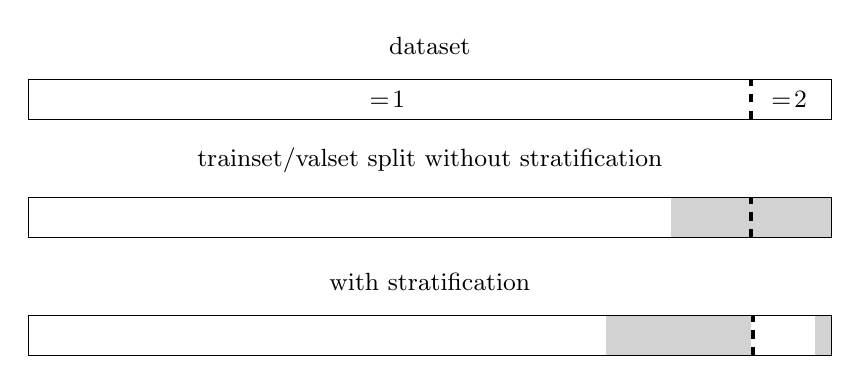
\begin{tikzpicture}[font=\small,x=1.7cm]
			% --- Parameters ---
			\def\cellw{6.0}     % total dataset width
			\def\cellh{0.5}     % height of one row
			\def\gap{1}       % vertical gap between rows
			\def\tfrac{0.8}     % train fraction
			\def\pA{0.9}        % proportion of stratum A (B = 1 - pA)
			% Column labels
			\node[anchor=south] at (0.5*\cellw, \cellh+0.2) {\gls{dataset}};
			\node[anchor=south] at ({0.5*\cellw}, {-(\cellh+\gap)+\cellh+0.2}) {\gls{trainset}/\gls{valset} split without stratification};
			\node[anchor=south] at (0.5*\cellw, {-2*(\cellh+\gap)+\cellh+0.2}) {with stratification};
			% y-positions
			\pgfmathsetmacro{\yDataset}{0}
			\pgfmathsetmacro{\yNoStrat}{-(\cellh+\gap)}
			\pgfmathsetmacro{\yStrat}{-2*(\cellh+\gap)}
			% A/B border x (dataset coordinate)
			\pgfmathsetmacro{\xAB}{\pA*\cellw}
			\pgfmathsetmacro{\wA}{\pA*\cellw}
			\pgfmathsetmacro{\wB}{(1-\pA)*\cellw}
			% --- Row 1: DATASET (only A/B border) ---
			\draw (0,\yDataset) rectangle ++(\cellw,\cellh);
			\draw[dashed,  line width=0.5mm] (\xAB,\yDataset) -- ++(0,\cellh);
			% Labels for strata in Dataset row
			\node at (0.5*\wA, \yDataset+0.5*\cellh) {$\sensattr\!=\!1$};
			\node at ({\xAB+0.5*\wB}, {\yDataset+0.5*\cellh}) {$\sensattr\!=\!2$};
			%	% --- Row 2: NO STRATIFICATION (shade right 20% as validation) ---
			\draw (0,\yNoStrat) rectangle ++(\cellw,\cellh);
			\pgfmathsetmacro{\xValStart}{\tfrac*\cellw}
			\pgfmathsetmacro{\valw}{(1-\tfrac)*\cellw}
			\fill[gray!35] (\xValStart,\yNoStrat) rectangle ++(\valw,\cellh);
			%	\fill[gray!35] (\xValStart,\yNoStrat) rectangle ++({(1-\tfrac)*\cellw,\cellh});
			%	% A/B border in dataset order only
			\draw[dashed,  line width=0.5mm] (\xAB,\yNoStrat) -- ++(0,\cellh);
			% --- Row 3: STRATIFIED (shade val inside each stratum A and B) ---
			\draw (0,\yStrat) rectangle ++(\cellw,\cellh);
			% A/B border at x = pA * cellw
			\pgfmathsetmacro{\xAB}{\pA*\cellw}
			\draw[dashed, line width=1mm] (\xAB,\yStrat) -- ++(0,\cellh);
			% widths of strata A and B
			% --- Validation area within A (right (1-tfrac) part of A) ---
			\pgfmathsetmacro{\xAVal}{\tfrac*\wA}              % start inside A (A begins at x=0)
			\pgfmathsetmacro{\wAVal}{(1-\tfrac)*\wA}          % width of A's validation
			\fill[gray!35] (\xAVal,\yStrat) rectangle ++(\wAVal,\cellh);
			% --- Validation area within B (right (1-tfrac) part of B) ---
			\pgfmathsetmacro{\xBVal}{\xAB + \tfrac*\wB}       % start inside B
			\pgfmathsetmacro{\wBVal}{(1-\tfrac)*\wB}          % width of B's validation
			\fill[gray!35] (\xBVal,\yStrat) rectangle ++(\wBVal,\cellh);
			\end{tikzpicture}
 		\caption{Stratification ensures that both the \gls{trainset} and the \gls{valset} 
			(shaded grey) have similar distributions of a binary key attribute $\sensattr$. 
			In other words, with stratification, both \glspl{stratum}  
			(i.e., $\sensattr\!=\!1$ and $\sensattr\!=\!2$ based on the key attribute) 
			allocate the same validation proportion—20\% of their own width. \label{fig_stratification_dict}}
 		\end{figure}
  		See also: \gls{stratum}, \gls{validation}, \gls{kfoldcv}.},
  	text={stratification},
  	first={stratification},
  	plural={stratifications}
}

\newglossaryentry{stratum}
{name={stratum},
	description={A\index{stratum} stratum is a subset of \glspl{datapoint} that all 
		share a common property (which could be a \gls{feature} or a \gls{label}). 
		For example, in a weather \gls{dataset}, all measurements from the same 
		\gls{fmi} weather station form one stratum.
		\begin{center}
			Example (CSV snippet):\\
  			{\ttfamily
  			time, station, value, unit\\
  			2023-06-01 12:00, Helsinki, 18.2, degree Celsius\\
  			2023-06-01 13:00, Helsinki, 18.5, degree Celsius\\
  			2023-06-01 14:00, Helsinki, 19.0, degree Celsius\\
  			2023-06-01 12:00, Oulu, 12.1, degree Celsius\\
  			2023-06-01 13:00, Oulu, 12.4, degree Celsius\\
  			2023-06-01 14:00, Oulu, 12.7, degree Celsius\\
  			2023-06-01 12:00, Tampere, 15.3, degree Celsius\\
  			2023-06-01 13:00, Tampere, 15.6, degree Celsius\\
  			2023-06-01 14:00, Tampere, 16.0, degree Celsius
  			}
		\end{center} 
		Here, the rows for each station (i.e., \texttt{Helsinki}, \texttt{Oulu}, \texttt{Tampere}) 
		represent different strata.
		\\ 
		See also: \gls{datapoint}, \gls{dataset}, \gls{stratification}.},
  	first={stratum},
  	firstplural={strata},
 	plural={strata}, 
 	text={stratum}
}

\newglossaryentry{attention}
{name={attention}, 
	description={Some \gls{ml} applications\index{attention} involve \glspl{datapoint} 
		composed of smaller units, referred to as \glspl{token}. For example, a sentence 
		consists of words, an image of pixel patches, and a network of nodes. In general, 
		the \glspl{token} that constitute a single \gls{datapoint} are not independent 
		of one another. Instead, each \gls{token} of a \gls{datapoint} depends on (or pays attention to) 
		specific other \glspl{token}. \Glspl{probmodel} provide a principled framework for 
		representing and analyzing such dependencies \cite{Blei2003}. Attention mechanisms use 
		a more direct approach without explicit reference to a \gls{probmodel}. The idea is to 
		represent the relationship between two \glspl{token} $\nodeidx$ and $\nodeidx'$ 
		using a parameterized \gls{function} $f^{(\weights)}(\nodeidx,\nodeidx')$, 
		where the \glspl{parameter} $\weights$ are learned via a variant of \gls{erm}. 
		Practical attention mechanisms differ in their precise choice of attention \gls{model} $f^{(\weights)}(\nodeidx,\nodeidx')$ 
		as well as in the precise \gls{erm} variant used to learn the \glspl{parameter} $\weights$. 
		One widely used family of attention mechanisms 
		defines the \glspl{parameter} $\weights$ in terms of two \glspl{vector} associated with each \gls{token} $\nodeidx$, i.e.,
		a query \gls{vector} $\vq^{(\nodeidx)}$ and a key \gls{vector} $\vk^{(\nodeidx')}$. For a given \gls{token} $\nodeidx$ 
		with query $\vq^{(\nodeidx)}$ and another \gls{token} $\nodeidx'$ with key $\vk^{(\nodeidx')}$, the quantity 
		$\big( \vq^{(\nodeidx)} \big)^{\top} \vk^{(\nodeidx')}$ indicates the extent to which \gls{token} $\nodeidx$ attends 
		to (or depends on) \gls{token} $\nodeidx'$ (see Fig. \ref{fig_attention_dict}).
		\begin{figure}[H]
			\centering
			\begin{tikzpicture}[>=stealth, node distance=0.2cm and 0.2cm,
			every node/.style={inner sep=2pt, font=\large}, baseline]
			% Words (sentence: All human beings are born free and equal.)
			\node (w1) [draw, fill=gray!10, rounded corners] {All};
			\node (w2) [draw, fill=gray!10, right=of w1, rounded corners] {human};
			\node (w3) [draw, fill=gray!10, right=of w2, rounded corners] {beings};
			\node (w4) [draw, fill=gray!10, right=of w3, rounded corners] {are};
			\node (w5) [draw, fill=gray!10, right=of w4, rounded corners] {born};
			\node (w6) [draw, fill=gray!10, right=of w5, rounded corners] {free};
			\node (w7) [draw, fill=gray!10, right=of w6, rounded corners] {and};
			\node (w8) [draw, fill=blue!20, right=of w7, rounded corners] {equal};
			% Label "i" below the word "equal"
   	   		\node[font=\footnotesize, below=0.15cm of w8, align=center] (labeli) {$\nodeidx$ \\ $\vq^{(\nodeidx)},\ \vk^{(\nodeidx)}$};
			\node[font=\footnotesize, below=0.15cm of w1, align=center] (labelii) {$\nodeidx'$ \\ $\vq^{(\nodeidx')},\ \vk^{(\nodeidx')}$};
			% Dummy node above for routing attention arrows
	  		\node (eqTop) [above=1.8cm of w8] {};
	 		% Arrows from "equal" to earlier words (drawn above)
	 		\draw[->, thick, opacity=0.3] (w8.north) .. controls +(up:1.0cm) and +(up:1.0cm) .. (w6.north); % to "free"
	 		\draw[->, thick, opacity=0.3] (w8.north) .. controls +(up:1.2cm) and +(up:1.0cm) .. (w5.north); % to "born"
			\draw[->, thick, opacity=1]  (w8.north)  .. controls +(up:1.8cm) and +(up:1.0cm) ..  node[midway, text=black, above] {$f^{(\weights)}(\nodeidx,\nodeidx')$}  (w1.north); % to "All"
			\end{tikzpicture}
			\caption{Attention mechanisms learn a parameterized \gls{function} $f^{(\weights)}(\nodeidx,\nodeidx')$ to measure 
				how much \gls{token} $\nodeidx$ attends to \gls{token} $\nodeidx'$. 
				One widely used construction of $f^{(\weights)}(\nodeidx,\nodeidx')$ 
				uses query and key \glspl{vector}, denoted by $\vq^{(\nodeidx)}$ and $\vk^{(\nodeidx)}$, assigned to each 
				\gls{token} $\nodeidx$ \cite{vaswani2017attention}. \label{fig_attention_dict}}
		\end{figure}
		See also: \gls{token}, \gls{function}, \gls{nlp}.},
	first={attention},
	text={attention}
}

\newglossaryentry{transformer}
{name={transformer},
	description={In the context of \gls{ml}, the term transformer\index{transformer} 
 		refers to an \gls{ann} that uses some form of \gls{attention} mechanism 
 		to capture dependencies among \glspl{token} \cite{vaswani2017attention}. 
 		The \gls{attention} mechanism is what sets transformers apart from 
		previous \glspl{model} used for sequential \gls{data} such as \glspl{rnn}. 
		A transformer \gls{ann} often combines several \gls{attention} \glspl{layer} 
		via more traditional \gls{layer} architectures. 
		\\ 
		See also: \gls{attention}, \gls{nlp}. }, 
 	first={transformer}, 
 	text={transformer},
 	firstplural={transformers}, 
 	plural={transformers}
}

\newglossaryentry{rnn}
{name={recurrent neural network (RNN)},
	description={An\index{recurrent neural network (RNN)} RNN 
  		is a specific type of \gls{ann} that is designed for processing 
    		\gls{data} that consist of a \gls{sequence} of \glspl{token}. 
		An RNN maintains an internal hidden \gls{state} that is updated recurrently 
		as new \glspl{token} are processed. This recurrent dependence allows 
		information to propagate across time steps, making RNNs suitable for 
		tasks such as speech recognition, language modeling, or time series \gls{prediction}. 
    		However, their inherently sequential computation limits parallelization and 
		is challenging for \glspl{gdmethod}. Variants like the long short-term memory (LSTM) 
		and gated recurrent unit (GRU) mitigate these problems.
		\\
		See also: \gls{ann}, \gls{token}. }, 
 	first={recurrent neural network (RNN)},
 	text={RNN},
 	firstplural={recurrent neural networks (RNNs)}, 
 	plural={RNNs}
}

\newglossaryentry{llm}
{name={large language model (LLM)},
	description={An\index{large language model (LLM)} LLM is an umbrella term for \gls{ml} 
		methods that use high-dimensional \gls{ml} \glspl{model} (with billions 
		of \glspl{modelparam}) trained on large collections of text \gls{data}. 
 		LLMs are used to analyze or generate \glspl{sequence} of \glspl{token} that 
               	constitute text \gls{data}. Many current LLMs use some variant of 
		a \gls{transformer} that is trained via \gls{selfsupervisedlearning}, i.e.,
		the \gls{training} is based on the task of predicting a few words that 
		are intentionally removed from a large text corpus. Thus, we can 
		construct \glspl{labeled datapoint} simply by selecting some words 
		from a given text as \glspl{label} and the remaining words as \glspl{feature} 
		of \glspl{datapoint}. This construction requires 
		very little human supervision and allows for generating sufficiently 
		large \glspl{trainset} for LLMs.
		\\ 
		See also: \gls{token}, \gls{transformer}, \gls{nlp}.}, 
  	first={large language model (LLM)}, 
  	firstplural={LLMs}, 
  	text={LLM}, 
  	plural={LLMs} 
}

\newglossaryentry{selfsupervisedlearning}
{name={self-supervised learning},
 	description={Self-supervised learning\index{self-supervised learning} uses some of 
  		the \glspl{feature} of a \gls{datapoint} as its \gls{label}. For 
		example, if a \gls{datapoint} consists of a sentence within a text document, 
		we can use the last word of the sentence as the \gls{label} that is 
		to be predicted from all the previous words, which form the \glspl{feature} 
		of the \gls{datapoint}. A main application of self-supervised learning 
		is in \gls{nlp} for the \gls{training} of \glspl{llm} from large collections 
		of text \gls{data}. 
		\\ 
      		See also: \gls{feature}, \gls{label}, \gls{llm}.}, 
   	first={self-supervised learning}, 
   	text={self-supervised learning}
}

\newglossaryentry{attack}
{name={attack},  
	description={An attack\index{attack} on an \gls{mlsystem} refers to an intentional \gls{action}—either 
		active or passive—that compromises the system's integrity, availability, or confidentiality. 
		Active attacks involve perturbing components such as \glspl{dataset} (via \gls{datapoisoning}) 
		or communication links between \glspl{device} within an \gls{ml} application. Passive attacks, 
		such as \glspl{privattack}, aim to infer \glspl{sensattr} without modifying the system. 
		Depending on their goal, we distinguish among \glspl{dosattack}, \gls{backdoor} attacks, and \glspl{privattack}.
		\\
		See also: \gls{datapoisoning}, \gls{privattack}, \gls{sensattr}, \gls{dosattack}, \gls{backdoor}.},
	plural={attacks}, 
	first={attack},
	firstplural={attacks},
	text={attack}
}

\newglossaryentry{privattack}
{name={privacy attack},
	description={A privacy \gls{attack}\index{privacy attack} on an \gls{mlsystem} aims to infer 
		\glspl{sensattr} of individuals by exploiting partial access to a trained \gls{ml} \gls{model}. 
		One form of a privacy \gls{attack} is \gls{modelinversion}.
		\\
		See also: \gls{attack}, \gls{sensattr}, \gls{modelinversion}, \gls{trustAI}, \gls{gdpr}.},
	plural={privacy attacks}, 
	first={privacy attack},
	firstplural={privacy attacks}, 
	text={privacy attack}
}

\newglossaryentry{discrepancy}
{name={discrepancy},
	description={Consider\index{discrepancy} an \gls{fl} application with \gls{netdata} 
		represented by an \gls{flnetwork}. \gls{fl} methods use a discrepancy \gls{measure} 
		to compare \gls{hypothesis} \glspl{map} from \glspl{localmodel} at nodes $\nodeidx,\nodeidx'$, 
		\gls{connected} by an edge in the \gls{flnetwork}.
					\\ 
		See also: \gls{fl}, \gls{flnetwork}, \gls{localmodel}.},
	first={discrepancy},
	firstplural={discrepancies}, 
  	plural={discrepancies}, 
	text={discrepancy}
}

\newglossaryentry{FedRelax}
{name={FedRelax},
	description={FedRelax refers to a \gls{gtvmin}-based \gls{fl} method\index{FedRelax} for training local \glspl{model} 
		at the \glspl{device} of an \gls{flnetwork} \cite{JungFLBook}. It is a 
		\gls{distributedalgorithm} that implements a nonlinear variant of the \gls{jacobimethod} to solve \gls{gtvmin}. 
		\\ 
		See also: \gls{fl}, \gls{distributedalgorithm}.},
	first={FedRelax},
	text={FedRelax}
}

\newglossaryentry{fedavg}
{name={federated averaging (FedAvg)},
	description={FedAvg\index{federated averaging (FedAvg)} refers to a family of iterative \gls{fl} \glspl{algorithm}. 
		It uses a server-client setting and alternates between clientwise \glspl{localmodel} 
		retraining, followed by the aggregation of updated \glspl{modelparam} at the server 
		\cite{pmlr-v54-mcmahan17a}, \cite{JungFLBook}. The local update at client $\nodeidx=1, \,\ldots, \,\nrnodes$ 
		at time $\iteridx$ starts from the current \glspl{modelparam} $\weights^{(\iteridx)}$ provided 
		by the server and typically amounts to executing few \glspl{iteration} of \gls{stochGD}. 
		After completing the local updates, they are aggregated 
		by the server (e.g., by averaging them). Fig. \ref{fig_single_iteration_fedavg_dict} illustrates 
		the execution of a single \gls{iteration} of FedAvg. 
		\begin{figure}[H]
			\begin{center}
			\begin{tikzpicture}[>=Stealth, node distance=1cm and 1.5cm, every node/.style={font=\small}]
			% Styles
			\tikzstyle{server} = [circle, fill=black, minimum size=6pt, inner sep=0pt]
			\tikzstyle{client} = [circle, draw=black, minimum size=6pt, inner sep=0pt]
			% Time step labels
			\node (label1) at (0,3.5) {broadcast};
			\node[right=2.5cm of label1] (label2) {local update};
			\node[right=2.5cm of label2] (label3) {aggregate};
			% Time step k
			\node[server] (s1) at (label1 |- 0,2.5) {};
			\node[client] (c1l) at ($(s1) + (-1cm,-1cm)$) {};
			\node[client] (c1r) at ($(s1) + (1cm,-1cm)$) {};
			\node[] (dots1) at ($(s1) + (0cm,-1cm)$) {\ldots};
			\draw[->] (s1) -- (c1l) node[midway,left] {$\weights^{(\iteridx)}$};
			\draw[->] (s1) -- (c1r) node[midway,right] {$\weights^{(\iteridx)}$};
			\draw[->] (s1) -- (dots1);
			% Time step k+1 (local updates)
			\node[server] (s2) at (label2 |- 0,2.5) {};
			\node[client] (c2l) at ($(s2) + (-1cm,-1cm)$) {};
			\node[client] (c2r) at ($(s2) + (1cm,-1cm)$) {};
			\node[] (dots2) at ($(s2) + (0cm,-1cm)$) {\ldots};
			\node[below=0.2cm of c2l] {$\localparamsiter{\iteridx}{1}$};
			\node[below=0.2cm of c2r] {$\localparamsiter{\iteridx}{\nrnodes}$};
			% Time step k+2 (aggregation)
			\node[server] (s3) at (label3 |- 0,2.5) {};
			\node[above=0.01cm of s3, yshift=-4pt] {$\weights^{(\iteridx+1)}$};
			\node[client] (c3l) at ($(s3) + (-1cm,-1cm)$) {};
			\node[client] (c3r) at ($(s3) + (1cm,-1cm)$) {};
			\node[] (dots3) at ($(s3) + (0cm,-1cm)$) {\ldots};
			\draw[->] (c3l) -- (s3) node[midway,left] {$\localparamsiter{\iteridx}{1}$};
			\draw[->] (c3r) -- (s3)  node[midway,right] {$\localparamsiter{\iteridx}{\nrnodes}$};
			\draw[->] (dots3) -- (s3);
			\end{tikzpicture}
			\end{center}
		\caption{Illustration of a single \gls{iteration} of FedAvg, which consists of broadcasting \glspl{modelparam} by the 
			server, performing local updates at clients, and aggregating the updates by the server. 
			\label{fig_single_iteration_fedavg_dict}} 
		\end{figure} 
		See also: \gls{fl}, \gls{algorithm}, \gls{localmodel}, \gls{stochGD}.},
	first={federated averaging (FedAvg)},
	text={FedAvg}
} 

\newglossaryentry{FedGD}
{name={federated gradient descent (FedGD)},
	description={FedGD refers to  an\index{federated gradient descent (FedGD)} \gls{fl} \gls{distributedalgorithm} that 
		can be implemented as message passing across an \gls{flnetwork} \cite{JungFLBook}. 
		\\ 
		See also: \gls{fl}, \gls{distributedalgorithm}, \gls{flnetwork}, \gls{gradstep}, \gls{gdmethod}.},
	first={federated gradient descent (FedGD)},
	text={FedGD}
} 

\newglossaryentry{FedSGD}
{name={federated stochastic gradient descent (FedSGD)},
	description={FedSGD refers to an\index{federated stochastic gradient descent (FedSGD)} \gls{fl} \gls{distributedalgorithm} that 
		can be implemented as message passing across an \gls{flnetwork} \cite{JungFLBook}. 
		\\ 
		See also: \gls{fl}, \gls{distributedalgorithm}, \gls{flnetwork}, \gls{gradstep}, \gls{gdmethod}, \gls{stochGD}.},
	first={federated stochastic gradient descent (FedSGD)},
	text={FedSGD}
} 

\newglossaryentry{hfl}
{name={horizontal federated learning (HFL)},
	description={HFL\index{horizontal federated learning (HFL)} uses \glspl{localdataset} constitut\-ed by different
	   	\glspl{datapoint} but uses the same \glspl{feature} to characterize them \cite{HFLChapter2020}.
		For example, weather forecasting uses a network of spatially distributed
		weather (observation) stations. Each weather station measures the
		same quantities, such as daily temperature, air pressure, and precipitation.
		However, different weather stations measure the characteristics or
		\glspl{feature} of different spatiotemporal regions. Each spatiotemporal region 
		represents an individual \gls{datapoint}, each characterized by the same \glspl{feature} 
		(e.g., daily temperature or air pressure).
		\\
		See also: \gls{ssl}, \gls{fl}, \gls{vfl}.},
	first={horizontal federated learning (HFL)},
	text={HFL}
} 

\newglossaryentry{dimred}
{name={dimensionality reduction},
	description={Dimensionality reduction\index{dimensionality reduction} refers 
		to methods that learn a transformation 
		$\hypothesis: \mathbb{R}^{\nrfeatures} \rightarrow \mathbb{R}^{\nrfeatures'}$ 
		of a (typically large) set of raw \glspl{feature} $\feature_{1}, \,\ldots, \,\feature_{\nrfeatures}$ 
		into a smaller set of informative \glspl{feature} $z_{1}, \,\ldots, \,z_{\nrfeatures'}$. 
		Using a smaller set of \glspl{feature} is beneficial in several ways: 
		\begin{itemize} 
			\item {Statistical benefit:} It typically reduces the \gls{risk} of \gls{overfitting}, as 
			reducing the number of \glspl{feature} often reduces the \gls{effdim} of a \gls{model}. 
			\item {Computational benefit:} Using fewer \glspl{feature} means less computation 
			for the \gls{training} of \gls{ml} \glspl{model}. As a case in point, \gls{linreg} methods 
			need to invert a \gls{matrix} whose size is determined by the number of \glspl{feature}. 
			\item {Visualization:} Dimensionality reduction is also instrumental for \gls{data} visualization. 
			For example, we can learn a transformation that delivers two \glspl{feature} $z_{1},z_{2}$, 
			which we can use, in turn, as the coordinates of a \gls{scatterplot}. Fig.\ \ref{fig:dimred-scatter_dict} 
			depicts the \gls{scatterplot} of handwritten digits that are placed 
			using transformed \glspl{feature}. Here, the \glspl{datapoint} are 
			naturally represented by a large number of greyscale values (one value for each pixel).
		\end{itemize} 
		 \begin{figure}[H]
		 \centering
		 \begin{tikzpicture}[scale=1]	
		% % Axes
		 	\draw[->] (-0.5,0) -- (5.5,0) node[right] {$z_1$};
		 	\draw[->] (0,-0.5) -- (0,4.5) node[above] {$z_2$};
		% % Example points with mini-images (can replace adjustbox with \includegraphics)
		 	\foreach \x/\y/\label in {
  		 		1.2/0.5/3,
  		 		0.8/2.0/8,
  		 		2.5/1.8/1,
  		 		3.8/3.5/6,
  		 		4.2/0.7/9,
  		 		2.8/3.0/7,
  		 		1.5/3.8/2
		 	}{
  		 		\node[draw, minimum size=0.6cm, inner sep=0pt] at (\x,\y)
    	 		{\label};
		 	}
		 	\end{tikzpicture}
		 	\caption{Example of dimensionality reduction: High-dimensional image \gls{data} 
			(e.g., high-resolution images of handwritten digits) embedded into 2-D using 
			learned \glspl{feature} $(z_1, z_2)$ and visualized in a \gls{scatterplot}.}
		 	\label{fig:dimred-scatter_dict}
		 \end{figure}
		See also: \gls{overfitting}, \gls{autoencoder}, \gls{randomprojection}, \gls{pca}, \gls{johnsonlindenstrausslemma}.}, 
	first={dimensionality reduction},
	text={dimensionality reduction}
} 

\newglossaryentry{diagnosis}
{name={diagnosis},
	description={Consider\index{diagnosis} an \gls{erm}-based method that resulted in a trained \gls{model} 
		(or learned \gls{hypothesis}) $\learnthypothesis \in \hypospace$. We can diagnose the 
		method by comparing the \gls{trainerr} $\trainerror$ with the \gls{valerr} $\valerror$ 
		incurred by $\learnthypothesis$ on the \gls{trainset} and the \gls{valset}. 
		\begin{figure}[H]
			\begin{center}
			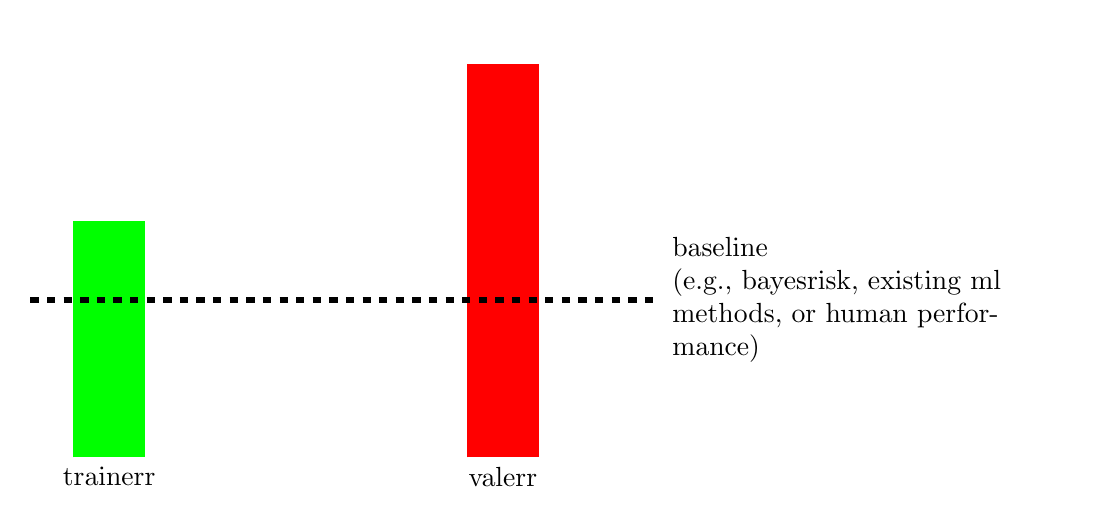
\begin{tikzpicture}[ycomb]
				\draw[color=green,line width=26pt]
				plot coordinates{(0,3)};
				\node [below] at (0,0) {\gls{trainerr}} ; 
				\draw[color=red,line width=26pt]
				plot coordinates{(5,5)};
				\node [below] at (5,0) {\gls{valerr}} ; 
				\draw[dashed,line width=2] (-1,2) -- (7,2) node[right,text width=5cm]{\gls{baseline} \\ (e.g., \gls{bayesrisk}, existing \gls{ml} methods, or human performance)};
			\end{tikzpicture}
			\end{center}
		\caption{We can diagnose an \gls{erm}-based \gls{ml} method by comparing its \gls{trainerr} 
			with its \gls{valerr}. Ideally, both are on the same level as a \gls{baseline}.\label{fig_diagnosis_dict}}
		\end{figure}
		See also: \gls{baseline}, \gls{validation}, \gls{kfoldcv}, \gls{generalization}.},
	first={diagnosis},
	text={diagnosis}
} 

\newglossaryentry{ml}
{name={machine learning (ML)},
	description={ML\index{machine learning (ML)} methods aim to learn (or find) 
		a useful \gls{hypothesis} \gls{map} $\learnthypothesis\!\in\!\hypospace$ out of 
		a \gls{model} $\hypospace$. The learned $\learnthypothesis$ is used to compute 
		a \gls{prediction} $\predictedlabel=\learnthypothesis(\featurevec)$ for 
		the \gls{label} $\truelabel$ of a \gls{datapoint}. The learning process is guided 
		by a quantitative \gls{measure} of the \gls{loss} incurred when  
		the \glspl{prediction} obtained from the learned \gls{hypothesis} differ from  
		the actual \gls{label} $\truelabel$. Different ML methods use different 
		design choices for this quantitative \gls{measure} (or \gls{lossfunc}) as well as 
		different choices for the \gls{model} and the \glspl{datapoint} (i.e., 
		their \glspl{feature} and \glspl{label}) \cite[Ch. 3]{MLBasics}. 
		\begin{figure}[H]
			\centering
			\hspace*{5mm}
			\begin{tikzpicture}[
				node distance=1cm,
				auto,
				punkt/.style={
				rectangle,
				rounded corners,
				draw=black,
				very thick,
				text width=3cm,
				minimum height=1cm,
				align=center
				}
				]
				\coordinate (OR) at (0.00, 1.50);
				% concentric circles
				\node[circle,inner sep=0,minimum size={6cm}](a) at (OR) {};
				\node[circle,inner sep=0,minimum size={8cm}](b) at (OR) {};
				\node[circle,inner sep=0,minimum size={8cm}](c) at (OR) {};
				% arcs and radii
				\draw[red,line width=1,dashed] (a.-150) arc (-150:{-150+120}:3cm);
				\draw[blue,line width=1,dashed] (b.160) arc (160:{160+50}:4cm);
				\draw[black!30!green,line width=2,dashed] (c.20) arc (20:{160}:4cm);
				\draw[black!30!blue,line width=2,dashed] ([shift={(-30:6cm)}]OR) arc (-30:{20}:6cm);
				\draw[black!30!blue,line width=2,dashed] (OR) --([shift={(-30:6cm)}]OR);
				\draw[black!30!blue,line width=2,dashed] (OR) --([shift={(20:6cm)}]OR);
				\draw[black!30!green,line width=2,dashed] (OR) -- (c.20);
				\draw[black!30!green,line width=2,dashed] (OR) -- (c.160);
				\draw[blue,thin,dashed] (OR) -- (b.160);
				\draw[blue,thin,dashed] (OR) -- (b.210);
				\draw[red,thin,dashed] (OR) -- (a.-150);
				\draw[red,thin,dashed] (OR) -- (a.-30);   
				% nodes
				\node[punkt] (data) {observations};
				\node[red,below=0.5cm of data] (data1) {\gls{data}};
				\node[above=of data] (dummy) {};
				\node[punkt,above=1cm of dummy] (hypothesis) {\gls{hypothesis}};
				\node[right=1.4cm of dummy] (t) {make a \gls{prediction}} ; 
				\node[left=1.4cm of dummy] (g) {assess and adapt} ;
				\node[blue,below=0.5cm of g,anchor=east] (g1) {\gls{loss}} ; 
				\node[black!30!blue,below=1cm of t,anchor=west] (g6) {\gls{inference}} ; 
				\node[black!30!green,above=1cm of hypothesis,anchor=south] (g3) {\gls{model}} ; 
				% arrows
				\draw [->,line width=0.5mm] (hypothesis.east) to [out=0,in=90] (t.north);
				\draw [->,line width=0.5mm] (t.south) to [out=270,in=0] (data.east);
				\draw [->,line width=0.5mm] (data.west) to [out=180,in=270] (g.south);
				\draw [->,line width=0.5mm] (g.north) to [out=90,in=180] (hypothesis.west);
			\end{tikzpicture}
			\vspace*{-9mm}
		\caption{ML learns a \gls{hypothesis} out of a \gls{model} (or \gls{hypospace}) 
			by trying to minimize the \gls{loss} incurred by the \glspl{prediction} 
			for the \glspl{label} of \glspl{datapoint}. The \glspl{prediction} are 
			computed solely from the \glspl{feature} of the \glspl{datapoint}.}
			\label{fig_AlexMLBP_dict}
		\end{figure}
		Another distinction between ML methods is how they access \glspl{datapoint} during 
		learning. For example, some methods have access to a complete \gls{dataset} 
		during \gls{training}, which allows them to use \gls{erm} \cite{MLBasics}, \cite{HastieWainwrightBook}. 
		In contrast, \gls{onlinelearning} methods access \gls{data} 
		sequentially and, in turn, update the learned \gls{hypothesis} 
		whenever a new \gls{datapoint} arrives \cite{PredictionLearningGames}, \cite{HazanOCO}, \cite{Bottou99}.
	 			\\ 
		See also: \gls{model}, \gls{loss}, \gls{data}, \gls{erm}, \gls{onlinelearning}.},
	first={machine learning (ML)},
	text={ML}
}

\newglossaryentry{featlearn}
{name={feature learning},
	description={Consider an \gls{ml} application with \glspl{datapoint} characterized by 
		raw \glspl{feature} $\featurevec \in \featurespace$. \Gls{feature} learning\index{feature learning} 
		refers to the task of learning a \gls{map} 
		$$\featuremapvec: \featurespace \rightarrow \featurespace': \featurevec \mapsto \featurevec'$$ 
		that reads in the \glspl{feature} $\featurevec \in \featurespace$ of a \gls{datapoint} and delivers new 
		\glspl{feature} $\featurevec' \in \featurespace'$ from a new \gls{featurespace} $\featurespace'$. 
		Different \gls{feature} learning methods are obtained for different design 
		choices of $\featurespace,\featurespace'$, for a \gls{hypospace} $\hypospace$ 
		of potential \glspl{map} $\featuremapvec$, and for a quantitative \gls{measure} of the usefulness of 
		a specific $\featuremapvec \in \hypospace$. For example, \gls{pca} 
		uses $\featurespace \defeq \mathbb{R}^{\dimlocalmodel}$, $\featurespace' \defeq \mathbb{R}^{\dimlocalmodel'}$ 
		with $\dimlocalmodel' < \dimlocalmodel$, and a \gls{hypospace} 
		$$\hypospace\defeq \big\{ \featuremapvec: \mathbb{R}^{\dimlocalmodel}
		\!\rightarrow\! \mathbb{R}^{\dimlocalmodel'}\!:\!\featurevec'\!\defeq\!\mF \featurevec \mbox{ with some } \mF \!\in\! \mathbb{R}^{\dimlocalmodel' \!\times \dimlocalmodel} \big\}.$$ 
		\Gls{pca} measures the usefulness of a specific \gls{map} $\featuremapvec(\featurevec)= \mF \featurevec$ 
		by the \gls{minimum} linear reconstruction error incurred on a \gls{dataset} such that 
		$$\min_{\mG \in \mathbb{R}^{\dimlocalmodel \!\!\!\times \dimlocalmodel'}} \sum_{\sampleidx=1}^{\samplesize} \normgeneric{\mG \mF \featurevec^{(\sampleidx)} - \featurevec^{(\sampleidx)}}{2}^{2}.$$ 
			\\ 
		See also: \gls{feature}, \gls{featurespace}, \gls{hypospace}, \gls{pca}.}, 
	first={feature learning},
	text={feature learning}
}

\newglossaryentry{encoder} 
{name={encoder}, 
	description={See \gls{autoencoder}\index{encoder}.}, 
 	first={encoder}, 
 	plural={encoders}, 
 	text={encoder}, 
 	firstplural={encoders}
}

\newglossaryentry{autoencoder}
{name={autoencoder},
	description={An autoencoder\index{autoencoder} is an \gls{ml} method that simultaneously 
		learns an \gls{encoder} \gls{map} $\hypothesis \in \hypospace$ and a decoder \gls{map} 
		$\hypothesis^{*} \in \hypospace^{*}$. Different autoencoders use different 
		\glspl{model} $\hypospace, \hypospace^{*}$, e.g., \glspl{ann} with different architectures. 
        		The special case of an autoencoder using (\gls{vector}-valued) \glspl{linmodel} for 
		$\hypospace, \hypospace^{*}$ results in \gls{pca}. 
		\begin{figure}[H]
			\centering
			\begin{tikzpicture}[>=Latex, thick, node distance=1.6cm]
			% Nodes
			\node (x) {$\vx$};
			\node[draw, rounded corners, right=of x, inner sep=4pt] (enc) {$\text{\gls{encoder} } \hypothesis$};
			\node[right=of enc] (z) {$\vz$};
			\node[draw, rounded corners, right=of z, inner sep=4pt] (dec) {$\text{decoder } \hypothesis^{*}$};
			\node[right=of dec] (xhat) {$\hat{\featurevec}$};
			% Arrows
			\draw[->] (x) -- (enc);
			\draw[->] (enc) -- node[above] {$\vz=\hypothesis(\featurevec)$} (z);
			\draw[->] (z) -- (dec);
			\draw[->] (dec) -- node[above] {$\hat{\featurevec}=\hypothesis^{*}(\vz)$} (xhat);
			% (Optional) reconstruction loss
			%\draw[->, dashed] ($(xhat.south)+(0,-0.2)$) to[bend right=20] node[below] {$\loss$} ($(x.south)+(0,-0.2)$);
			\end{tikzpicture}
		\caption{Autoencoder with an \gls{encoder} $\hypothesis$ mapping $\featurevec \mapsto \vz$ and 
			a decoder $\hypothesis^*$ mapping $\vz \mapsto \hat{\featurevec}$.}
		\end{figure}
		The \gls{training} of the \gls{encoder} and decoder can be implemented via \gls{erm} using a \gls{loss} that measures 
		the deviation of the reconstructed \gls{featurevec} $\hypothesis^{*}\big(\hypothesis\big(\featurevec \big) \big)$
		from the original \gls{featurevec} $\featurevec$.
					\\ 
		See also: \gls{encoder}, \gls{featlearn}, \gls{dimred}.},
	first={autoencoder},
	text={autoencoder}
} 

\newglossaryentry{modelparallelism}
{name={model parallelism},
	description={\Gls{model} parallelism\index{model parallelism} refers to a particular 
        		class of distributed \glspl{optmethod} used to train an \gls{ml} \gls{model}.  
		Here, different \glspl{device} store and process disjoint subsets of the 
             	\glspl{modelparam}. This approach contrasts with \gls{dataparallelism}, where each 
             	\gls{device} maintains a full replica of the \glspl{modelparam} while 
             	processing disjoint subsets of the global \gls{dataset}. 
             	\Gls{model} parallelism allows us to train an \gls{ml} \gls{model} whose 
		\glspl{parameter} cannot fit into the memory of a single \gls{device}. 
             	One key application of \gls{model} parallelism is the \gls{training} of 
            	extremely large \glspl{ann}, such as \gls{transformer} \glspl{model} with 
             	billions of \glspl{modelparam}. 
             	\\
             	See also: \gls{vfl}.},
 	first={model parallelism},
 	text={model parallelism}
}

\newglossaryentry{dataparallelism}
{name={data parallelism},
	description={\Gls{data} parallelism\index{data parallelism} refers to a widely used 
 		class of distributed \glspl{optmethod} for \gls{training} an \gls{ml} 
             	\gls{model}. Here, each participating \gls{device} stores a full 
             	replica of the \glspl{modelparam} but processes a disjoint subset of 
             	the global \gls{dataset} \cite{DistrOptStatistLearningADMM}. 
             	Compared to \gls{modelparallelism}, which distributes the 
             	\glspl{modelparam} across \glspl{device}, \gls{data} parallelism distributes 
             	the computational workload associated with large \glspl{dataset}. 
             	It is especially effective when the \gls{model} fits into the memory 
             	of a single \gls{device}, but the \gls{dataset} or \gls{training} complexity 
		would be prohibitive without parallel processing. 
             	\\
             	See also: \gls{modelparallelism}, \gls{hfl}.},
 	first={data parallelism},
 	text={data parallelism}
}

\newglossaryentry{perplexity}
{name={perplexity},
	description={The\index{perplexity} perplexity of an \gls{rv} $x$ is defined as $e^{H_{x}}$.
         	\\
             	See also: \gls{entropy}.},
 	first={perplexity},
 	text={perplexity}
}

\newglossaryentry{vfl}
{name={vertical federated learning (VFL)},
	description={In VFL,\index{vertical federated learning (VFL)} different \glspl{device} have 
		access to different \glspl{feature} of the same set of \glspl{datapoint} \cite{VFLChapter}. 
		Formally, the underlying global \gls{dataset} is
		\[
		\dataset^{(\mathrm{global})} \defeq \left\{ \left(\featurevec^{(1)}, \truelabel^{(1)}\right), \,\ldots, \,\left(\featurevec^{(\samplesize)}, \truelabel^{(\samplesize)}\right) \right\}.
		\]
		We denote by $\featurevec^{(\sampleidx)} = \big( \feature^{(\sampleidx)}_{1}, \,\ldots, \,\feature^{(\sampleidx)}_{\nrfeatures'} \big)\,^{T}$, for $\sampleidx=1, \,\ldots, \,\samplesize$, 
	     	the complete \glspl{featurevec} for the \glspl{datapoint}. Each \gls{device} $\nodeidx \in \nodes$ 
		observes only a subset $\mathcal{F}^{(\nodeidx)} \subseteq \{1, \,\ldots, \,\nrfeatures'\}$ of \glspl{feature}, resulting 
		in a \gls{localdataset} $\localdataset{\nodeidx}$ with \glspl{featurevec}
		\[
		\featurevec^{(\nodeidx,\sampleidx)} = \big( \feature^{(\sampleidx)}_{\featureidx_{1}}, \,\ldots, \,\feature^{(\sampleidx)}_{\featureidx_{\nrfeatures}} \big)\,^{T}.
		\]
		Some of the \glspl{device} may also have access to the \glspl{label} $\truelabel^{(\sampleidx)}$, for $\sampleidx=1, \,\ldots, \,\samplesize$, 
		of the global \gls{dataset} (see Fig. \ref{fig_vertical_FL_dict}). 
		\begin{figure}[H]
			\begin{center}
			\begin{tikzpicture}[every node/.style={anchor=base}]
				  % --- Coordinate definitions ---
				\def\colX{0}
				\def\colY{1.6}
				\def\colZ{3.2}
				\def\colD{4.8}
				\def\colLabel{6.4} 
				\def\rowOne{0}
				\def\rowTwo{-1.2}
				\def\rowThree{-2.4}
				\def\rowFour{-3.6}
				% Manually place matrix entries
				\foreach \i/\label in {1/1, 2/2, 4/\samplesize} {
					\pgfmathsetmacro{\y}{-1.2*(\i-1)}
					\node (x\i1) at (0,\y) {$x^{(\label)}_{1}$};
					\node (x\i2) at (1.6,\y) {$x^{(\label)}_{2}$};
					\node (dots\i) at (3.2,\y) {$\cdots$};
					\node (x\i3) at (4.8,\y) {$x^{(\label)}_{\dimlocalmodel}$};
					\node (y\i) at (6.4,\y) {$\truelabel^{(\label)}$};
				}
				% Outer rectangle for the full dataset
				\draw[dashed, rounded corners, thick]
				(-0.6,0.6) rectangle (6.9,-4.2);
				\node at (3.1,0.9) {$\dataset^{(\mathrm{global})} $};
				% Rectangle for local dataset 1 (e.g., first two features)
				\draw[dashed, rounded corners, thick]
				(-0.9,0.9) rectangle (2.1,-4.0);
				\node at (0.25,1.0) {$\localdataset{1}$};
		  		% --- Local dataset k (columns 2–3, rows 1–3) ---
				\draw[dashed, rounded corners, thick]
				($( \colZ + 1,,0.9 )$) rectangle
				($( \colLabel + 0.4, -4.5)$);
				\node at ($( \colZ + 0.9,-5 )$) {$\localdataset{\nodeidx}$};
			\end{tikzpicture}
			\end{center}
		\caption{VFL uses \glspl{localdataset} that are derived from the \glspl{datapoint} of a common global \gls{dataset}. 
			The \glspl{localdataset} differ in the choice of \glspl{feature} used to characterize 
			the \glspl{datapoint}.\label{fig_vertical_FL_dict}}
		\end{figure}
		One potential application of VFL is to enable collaboration between 
		different healthcare providers. Each provider collects distinct types of measurements—such as blood 
		values, electrocardiography, and lung X-rays—for the same patients. Another 
		application is a national social insurance system, where health records, financial 
		indicators, consumer behavior, and mobility \gls{data} are collected by different 
		institutions. VFL enables joint learning across these parties while allowing 
		well-defined levels of \gls{privprot}. We can view VFL as a specific form of
		\gls{modelparallelism}.
		\\
		See also: \gls{privprot}, \gls{fl}, \gls{modelparallelism}.},
	first={vertical federated learning (VFL)},
	text={VFL}
} 

\newglossaryentry{interpretability}
{name={interpretability},
	description={An \gls{ml} method is interpretable\index{interpretability} for a 
 		human user if they can comprehend the decision process of the method. 
		One approach to develop a precise definition of interpretability is via the concept  
 		of simulatability, i.e., the ability of a human to mentally simulate the \gls{model} behavior 
		\cite{Colin:2022aa}, \cite{Chen2018}, \cite{doshi2017towards}, \cite{hase-bansal-2020-evaluating}, \cite{Lipton2018}. 
 		The idea is as follows: If a human user understands an \gls{ml} method, then they should 
 		be able to anticipate its \glspl{prediction} on a \gls{testset}. We illustrate 
 		such a \gls{testset} in Fig. \ref{fig_aug_simulatability_dict}, which also depicts 
		two learned \glspl{hypothesis} $\learnthypothesis$ and $\learnthypothesis'$. 
		The \gls{ml} method producing the \gls{hypothesis} $\learnthypothesis$ is interpretable
		to a human user familiar with the concept of a \gls{linearmap}. 
    		Since $\learnthypothesis$ corresponds to a \gls{linearmap}, the user can 
		anticipate the \glspl{prediction} of $\learnthypothesis$ on the 
		\gls{testset}. In contrast, the \gls{ml} method delivering $\learnthypothesis'$ 
		is not interpretable, because its behavior is no longer aligned with the user’s 
		\glspl{expectation}.
 		\begin{figure}[H]
 			\begin{center} 
			\begin{tikzpicture}[x=1.5cm, y=1cm]
  			% Adjustable parameters
 			\def\slope{0.4}
  			\def\offset{2.0}
  			% Axes
  			\draw[->, very thick] (0,0.5) -- (7.7,0.5) node[below, xshift=-1cm] {$\feature$}; % x-axis
 			\draw[->, very thick] (0.5,0) -- (0.5,4.2) node[above] {$\truelabel$};           % y-axis
  			% Model line
  			\draw[color=black, thick, dashed, domain=-0.5:7.2, variable=\x] 
    			plot ({\x},{\slope*\x + \offset});
			% non-interpretable model
  			\draw[color=black, thick, dashed, domain=4:7.2, variable=\x] 
    			plot ({\x},{\slope*\x + \offset-(\x-4)*0.5});
  			\node[above] at (7.2, {\slope*7.2 + \offset}) {$\learnthypothesis(\feature)$};
  			\node[above] at (7.2, {\slope*7.2 + \offset - 0.5*(7.2 - 4)}) {$\learnthypothesis'(\feature)$};
 			%\node[above] at (7.2, {\slope*7.2 + \offset-(7.2-4)*0.3}) {$\learnthypothesis'(\feature)$};
  			% Training Data points
  			\foreach \x/\y/\c/\s in {
      			1.2/1.0/blue/6, 1.4/1.0/blue/6, 1.7/1.0/blue/6,
      			2.2/3.9/blue/12, 2.6/4.2/blue/12, 3.0/4.4/blue/12
  			}{
    			\coordinate (pt) at (\x,\y);
    			\node[fill=\c, circle, draw, minimum size=\s pt, scale=0.6] at (pt) {};
    			\draw[<->, >={Latex[width=2mm,length=4mm]}, color=\c, thick]
      			(\x, {\slope*\x + \offset}) -- (pt);
  			}
  			% test set with pseudo-labels
    			\foreach \x/\y/\c/\s in {
       			5.7/2.6/red/12, 5.9/2.6/red/12, 6.2/2.6/red/12
   			}{
     			\coordinate (pt) at (\x,{\slope*\x + \offset});
     			\node[fill=\c, circle, draw, minimum size=\s pt, scale=0.6] at (pt) {};
   			}
  			% Legend
  			\draw[fill=blue] (4.2, 1.7) circle (0.1cm) node [black,xshift=0.2cm,anchor=west] {\gls{trainset} $\dataset$};
  			\draw[fill=red]  (4.2, 1.2) circle (0.1cm) node [black,xshift=0.2cm,anchor=west] {\gls{testset} $\dataset'$};
			\end{tikzpicture}
 			\caption{We can assess the interpretability of trained \gls{ml} \glspl{model} 
 			$\learnthypothesis$ and $\learnthypothesis'$ by comparing their \glspl{prediction} 
			to pseudo-\glspl{label} generated by a human user for $\dataset'$. 
			\label{fig_aug_simulatability_dict}}
 			\end{center}
	 	\end{figure} 
 	 	The notion of interpretability is closely related to the notion of \gls{explainability}, 
 	 	as both aim to make \gls{ml} methods more understandable for humans. 
		In the context of Fig. \ref{fig_aug_simulatability_dict}, interpretability of an \gls{ml} 
	 	method $\learnthypothesis$ requires that the human user can anticipate its \glspl{prediction} 
	 	on an arbitrary \gls{testset}. This contrasts with \gls{explainability}, where the user is supported by 
	 	external \glspl{explanation}—such as saliency \glspl{map} or reference examples from the \gls{trainset}—to 
		understand the \glspl{prediction} of $\learnthypothesis$ on a specific \gls{testset} $\dataset'$. 
	 	\\ 
	 	See also: \gls{explainability}, \gls{trustAI}, \gls{regularization}, \gls{lime}. },
	first={interpretability},
 	text={interpretability}
}

\newglossaryentry{multitask learning}
{name={multitask learning},
	description={Multitask learning\index{multitask learning} aims to leverage relations between 
	 	different \glspl{learningtask}. Consider two \glspl{learningtask} obtained from the 
	 	same \gls{dataset} of webcam snapshots. The first task is to predict the presence 
	 	of a human, while the second task is to predict the presence of a car. It may be useful 
	 	to use the same \gls{deepnet} structure for both tasks and only allow the \glspl{weight} of 
	 	the final \gls{output} \gls{layer} to be different.
	 			\\ 
		See also: \gls{learningtask}, \gls{dataset}, \gls{deepnet}, \gls{weight}, \gls{layer}.},
	first={multitask learning},
	text={multitask learning}
}

\newglossaryentry{learningtask}
{name={learning task},
	description={Consider\index{learning task} a \gls{dataset} $\dataset$ consisting of 
		multiple \glspl{datapoint} $\datapoint^{(1)},\,\ldots,\,\datapoint^{(\samplesize)}$. 
		For example, $\dataset$ can be a collection of images in an image database. 
		A learning task is defined by specifying those properties (or attributes) of a \gls{datapoint} 
		that are used as its \glspl{feature} and \glspl{label}. Given a choice of \gls{model} $\hypospace$ and 
		\gls{lossfunc}, a learning task leads to an instance of \gls{erm} and can thus be 
		represented by the associated \gls{objfunc} $\emprisk{\hypothesis}{\dataset}$ for $\hypothesis \in \hypospace$. 
		Importantly, multiple distinct learning tasks can be constructed from the same \gls{dataset} 
		by selecting different sets of \glspl{feature} and \glspl{label} (see Fig. \ref{fig:learning_tasks_cows_dict}).
    		\begin{figure}[H]
			\centering
			% Top row: image
			\begin{minipage}[t]{0.95\textwidth}
    			\centering
    			\includegraphics[width=\textwidth]{assets/CowsAustria.jpg}
    			\caption*{An image showing cows grazing in the Austrian countryside.}
			\vspace{5mm}
			\end{minipage}
			\vspace{5mm}
			% Bottom row: two learning tasks
			\begin{minipage}[t]{0.45\textwidth}
    			Task 1 (\gls{regression}): \\
        			\Glspl{feature} are the RGB values of all image pixels,
        			and the \gls{label} is the number of cows depicted.
			\end{minipage}
			\hfill
			\begin{minipage}[t]{0.45\textwidth}
    			Task 2 (\gls{classification}): \\
			\Glspl{feature} include the average green intensity of the image, 
        			and the \gls{label} indicates whether cows should be moved to another location (i.e., yes/no).
			\end{minipage}
			\caption{Two learning tasks constructed from a single image \gls{dataset}. 
			These tasks differ in \gls{feature} selection and choice of \gls{label} (i.e., the objective), 
			but are both derived from the same \gls{dataset}.}
			\label{fig:learning_tasks_cows_dict}
		\end{figure}
		Different learning tasks arising from the same underlying \gls{dataset} are often coupled. 
		For example, when a \gls{probmodel} is used to generate \glspl{datapoint}, statistical 
		dependencies among different \glspl{label} induce dependencies among the corresponding 
		learning tasks. In general, solving learning tasks jointly, e.g., using \gls{multitask learning} 
		methods, tends to be more effective than solving them independently (thereby ignoring 
		dependencies among learning tasks) \cite{Caruana:1997wk}, \cite{JungGaphLassoSPL}, \cite{CSGraphSelJournal}.
	 			\\ 
		See also: \gls{multitask learning}, \gls{labelspace}.},
	first={learning task},
	firstplural={learning tasks},
	plural={learning tasks}, 
	text={learning task}
}

\newglossaryentry{explainability}
{name={explainability},
	description={We\index{explainability} define the (subjective) explainability of an \gls{ml} method 
		as the level of simulatability \cite{Colin:2022aa} of the \glspl{prediction} 
		delivered by an \gls{mlsystem} to a human user. Quantitative \glspl{measure} of the 
		(subjective) explainability of a trained \gls{model} can be constructed by 
		comparing its \glspl{prediction} with the \glspl{prediction} provided by a user 
		on a \gls{testset} \cite{Colin:2022aa}, \cite{Zhang:2024aa}. Alternatively, we can use 
		\glspl{probmodel} for \gls{data} and measure the explainability of a trained \gls{ml} 
		\gls{model} via the conditional (or differential) \gls{entropy} of its \glspl{prediction}, given the 
		user's \glspl{prediction} \cite{JunXML2020}, \cite{Chen2018}.
						\\ 
		See also: \gls{trustAI}, \gls{regularization}.},
	first={explainability},
	text={explainability}
}

\newglossaryentry{lime}
{name={local interpretable model-agnostic explanations (LIME)},
	description={Consider\index{local interpretable model-agnostic explanations (LIME)} 
		a trained \gls{model} (or learned \gls{hypothesis}) $\widehat{\hypothesis} \in \hypospace$, 
		which maps the \gls{featurevec} of a \gls{datapoint} to the \gls{prediction} $\widehat{\truelabel}= \widehat{\hypothesis}$. 
		LIME is a technique for explaining the behavior of $\widehat{\hypothesis}$ 
		locally around a \gls{datapoint} with \gls{featurevec} $\featurevec^{(0)}$ \cite{Ribeiro2016}. 
		The \gls{explanation} is given in the form of a local approximation $g \in \hypospace'$ of $\widehat{\hypothesis}$ 
		(see Fig. \ref{fig_lime_dict}). This approximation can be obtained by an instance of \gls{erm} 
		with a carefully designed \gls{trainset}. In particular, the \gls{trainset} consists of \glspl{datapoint} with 
		\glspl{featurevec} centered around $\featurevec^{(0)}$ and the (pseudo-)\gls{label} $\widehat{\hypothesis}(\featurevec)$. 
		Note that we can use a different \gls{model} $\hypospace'$ for the approximation from 
		the original \gls{model} $\hypospace$. For example, we can use a \gls{decisiontree} 
		to locally approximate a \gls{deepnet}. Another widely used choice for $\hypospace'$ is 
		the \gls{linmodel}. 
		\begin{figure}[H]
		\begin{center}
		\begin{tikzpicture}
			\begin{axis}[
				axis lines=middle,
				xlabel={$\featurevec$},
				ylabel={$\truelabel$},
				xtick=\empty,
				ytick=\empty,
				xmin=0, xmax=6,
				ymin=0, ymax=6,
				domain=0:6,
				samples=100,
				width=10cm,
				height=6cm,
				clip=false
			]
			% Nonlinear model h(x)
  			\addplot[blue, thick, domain=0:6] {2 + sin(deg(x))} node[pos=0.85, above right,yshift=3pt] {$\widehat{\hypothesis}(\featurevec)$};
			% Feature value x0
  			\addplot[dashed, gray] coordinates {(3,0) (3,6)};
			% Piecewise constant local approximation g(x)
  			\addplot[red, thick, domain=2.5:3.5] {2 + sin(deg(3))} node[pos=0.9, above] {$g(\featurevec)$};
			% Optional: mark the point of approximation
  			\addplot[mark=*] coordinates {(3, {2 + sin(deg(3))})};
			\node at (axis cs:3,-0.3) {$\featurevec^{(0)}$};
			\end{axis}
		\end{tikzpicture}
		\end{center}
		\caption{To explain a trained \gls{model} $\widehat{\hypothesis} \in \hypospace$, around a 
			given \gls{featurevec} $\featurevec^{(0)}$, we can use a local approximation $g \in \hypospace'$. }
			\label{fig_lime_dict}
		\end{figure}
		See also: \gls{model}, \gls{explanation}, \gls{erm}, \gls{trainset}, \gls{label}, \gls{decisiontree}, \gls{deepnet}, \gls{linmodel}.},
	first={LIME},
	text={LIME}
}

\newglossaryentry{linmodel}
{name={linear model}, 
	description={Consider\index{linear model} an \gls{ml} application involving \glspl{datapoint}, each represented 
		by a numeric \gls{featurevec} $\featurevec \in \mathbb{R}^{\nrfeatures}$. A linear \gls{model} defines 
		a \gls{hypospace} consisting of all real-valued \glspl{linearmap} from $\mathbb{R}^{\nrfeatures}$ to $\mathbb{R}$ such that
		\begin{equation}
			\nonumber
			\label{equ_def_lin_model_hypspace_dict}
			\linmodel{\nrfeatures} \defeq \left\{ \hypothesis: \mathbb{R}^{\nrfeatures} \rightarrow \mathbb{R} \mid \hypothesis(\featurevec) = \weights^{\top} \featurevec \text{ for some } \weights \in \mathbb{R}^{\nrfeatures} \right\}.
		\end{equation}
		Each value of $\nrfeatures$ defines a different \gls{hypospace}, corresponding to the number of 
		\glspl{feature} used to compute the \gls{prediction} $\hypothesis(\featurevec)$. The choice of 
		$\nrfeatures$ is often guided not only by \glspl{compasp} (e.g., fewer \glspl{feature} reduce computation) and 
		\glspl{statasp} (e.g., more \glspl{feature} typically reduce \gls{bias} and \gls{risk}), but also by \gls{interpretability}. 
		A linear \gls{model} using a small number of well-chosen \glspl{feature} is generally considered 
		more interpretable \cite{rudin2019stop}, \cite{Ribeiro2016}.
		The linear \gls{model} is attractive because it can typically be trained using scalable \gls{convex} 
		\glspl{optmethod} \cite{BertsekasNonLinProgr}, \cite{hastie01statisticallearning}. 
		Moreover, linear \glspl{model} often permit rigorous 
		statistical analysis, including fundamental limits on the \gls{minimum} achievable \gls{risk} \cite{Wain2019}. 
		They are also useful for analyzing more complex nonlinear \glspl{model} such as \glspl{ann}. For instance, 
		a \gls{deepnet} can be viewed as the composition of a \gls{featuremap}—implemented by the input and 
		hidden \glspl{layer}—and a linear \gls{model} in the \gls{output} \gls{layer}. Similarly, a \gls{decisiontree} can be interpreted 
		as applying a one-hot-encoded \gls{featuremap} based on \glspl{decisionregion}, followed by a linear 
		\gls{model} that assigns a \gls{prediction} to each region.
		More generally, any trained \gls{model} $\learnthypothesis \in \hypospace$ that is 
		\gls{differentiable} at some $\featurevec'$ can be locally approximated by a \gls{linearmap} 
		$g(\featurevec)$. Fig.~\ref{fig_linapprox_dict} illustrates such a local linear approximation, 
		defined by the \gls{gradient} $\nabla \learnthypothesis(\featurevec')$. Note that the \gls{gradient} 
		is only defined where $\learnthypothesis$ is \gls{differentiable}.
		To ensure \gls{robustness} in the context of \gls{trustAI}, one may prefer \glspl{model} whose 
		associated \gls{map} $\learnthypothesis$ is Lipschitz \gls{continuous}. A classic result in mathematical 
		analysis—Rademacher’s theorem—states that if $\learnthypothesis$ is Lipschitz \gls{continuous} with 
		some constant $L$ over an open set $\samplespace \subseteq \mathbb{R}^{\nrfeatures}$, then $\learnthypothesis$ 
		is \gls{differentiable} almost everywhere in $\samplespace$ \cite[Th.~3.1]{heinonen2005lectures}.
		\begin{figure}[H]
			\begin{center}
			\begin{tikzpicture}[x=0.5cm]
			\begin{axis}[
			hide axis,
			xmin=-3, xmax=6,
			ymin=0, ymax=6,
			domain=0:6,
			samples=100,
			width=10cm,
			height=6cm,
			clip=false
			]
			% Original nonlinear function h(x)
			\addplot[blue, thick, domain=-2:6] {2 + sin(deg(x))} 
			node[pos=0.5, above right, yshift=3pt] {$\learnthypothesis(\featurevec)$};
			% Tangent line as local linear approximation at x = 3
			% h(3) = 2 + sin(3), h'(3) = cos(3)
			\addplot[red, thick, domain=4.5:6.5] 
			{2 + sin(deg(6)) + cos(deg(6))*(x - 6)}
			node[pos=0.95, above right] {$g(\featurevec)$};
			% Mark point of approximation
			\addplot[mark=*] coordinates {(6, {2 + sin(deg(6))})};
			% Vertical dashed line (ruler) at x = 3
			\addplot[dashed, gray] coordinates {(6,0) (6,2.4)};
			\node at (axis cs:6, -0.2) {$\featurevec'$};
			% Plot the two points
			% Coordinates of the two points
			\pgfmathsetmacro{\xA}{-1.5}
			\pgfmathsetmacro{\xB}{3}
			\pgfmathsetmacro{\yA}{2 + sin(deg(\xA))}
			\pgfmathsetmacro{\yB}{2 + sin(deg(\xB))}
			\addplot[mark=*, only marks] coordinates {(\xA, \yA) (\xB, \yB)};
			%	\node at (axis cs:\xA, \yA+0.2) {$A$};
			%	\node at (axis cs:\xB, \yB+0.2) {$B$};
			% Draw dashed lines from the points to the x and y axes
			\draw[dashed, gray] (axis cs:\xA,\yA) -- (axis cs:\xA,0);
			\draw[dashed, gray] (axis cs:\xB,\yB) -- (axis cs:\xB,0);
			\draw[dashed, gray] (axis cs:\xA,\yA) -- (axis cs:0,\yA);
			\draw[dashed, gray] (axis cs:\xB,\yB) -- (axis cs:0,\yB);
			 % Draw delta x
			\draw[<->, thick] (axis cs:\xA,-0.4) -- node[below] {$\normgeneric{\Delta \featurevec}{2}$} (axis cs:\xB,-0.4);
			% Draw delta y
			\draw[<->, thick] (axis cs:-2.4,\yA) -- node[left] {$\leq L \normgeneric{\Delta \featurevec}{2}$} (axis cs:-2.4,\yB);
			\end{axis}
			\vspace*{-10mm}
			\end{tikzpicture}
			\vspace*{-5mm}
			\end{center}
		\caption{A trained \gls{model} $\learnthypothesis(\featurevec)$ that is \gls{differentiable} at a point $\featurevec'$ 
			can be locally approximated by a \gls{linearmap} $g \in \linmodel{\nrfeatures}$. This local approximation 
			is determined by the \gls{gradient} $\nabla \learnthypothesis(\featurevec')$.}
			\label{fig_linapprox_dict}
		\end{figure}
		See also: \gls{model}, \gls{hypospace}, \gls{linearmap}, \gls{interpretability}, \gls{lime}.}, 
   first={linear model},
   plural={linear models},
   firstplural={linear models}, 
   text={linear model}
}

\newglossaryentry{earlystopping}
{name={early stopping}, 
	description={Consider an \gls{erm}-based method that uses an 
		iterative \gls{optmethod} (such as \gls{gd}) to learn \glspl{modelparam} 
		by minimizing the \gls{emprisk} on a given \gls{trainset}.
		Early stopping\index{early stopping} refers to terminating the \glspl{iteration} 
		even if they still substantially decrease the \gls{emprisk} on the 
		\gls{trainset}. Instead of monitoring the \gls{objfunc} (which is the 
		\gls{emprisk} on the \gls{trainset}), early stopping monitors the \gls{valerr} 
		incurred by the \glspl{modelparam} in each \gls{iteration}. Early stopping can be 
		interpreted as an implementation of \gls{regularization} via \gls{model} 
		pruning. Indeed, terminating an iterative \gls{optmethod} after a small number 
		of \glspl{iteration} restricts the set of \glspl{modelparam} that can be reached from the 
		initialization (see Fig.\ \ref{fig_early_stopping_dict}).
		\begin{figure}[H]
		\centering
			\begin{tikzpicture}[>=Stealth, scale=2]
			% Initialization
			\fill (0,0) circle (0.6pt) node[above] {\small $\weights^{(0)}$};
			\node at (-0.4,0) {\small $\hypospace^{(1)}$};
			\node at (-1.2,0) {\small $\hypospace^{(2)}$};
			\node at (-2,0) {\small $\hypospace \ldots$};
			% T-step reachable sets (early stopping = smaller T)
			\draw[densely dotted] (0,0) ellipse (0.8 and 0.4);
			\draw[dashed] (0,0) ellipse (1.6 and 0.8);
			% Example gradient path (just illustrative)
			\draw[->] (0,0) -- (0.8,0.) node [pos=0.6,above] {\tiny $1$ step};
			\draw[->] (0.0,0.0) -- (0,-0.8) node [pos=0.9,right] {\tiny $2$ steps};
			\end{tikzpicture}
		\caption{A \gls{gdmethod} for \gls{erm} using a \gls{hypospace} $\hypospace$ 
		    	defines a nested \gls{sequence} of effective \glspl{hypospace} 
			$\hypospace^{(1)} \subseteq \hypospace^{(2)} \subseteq \ldots \subseteq \hypospace$. 
			The effective \gls{hypospace} $\hypospace^{(\iteridx)}$ is 
		    	determined by all \glspl{modelparam} that can be reached from the initialization 
			$\weights^{(0)}$ within $\iteridx$ \glspl{gradstep}. \label{fig_early_stopping_dict}}
		\end{figure}
		See also: \gls{regularization}, \gls{gdmethod}, \gls{overfitting}.},
	first={early stopping},
	text={early stopping}
}

\newglossaryentry{statasp}
{name={statistical aspect}, 
	description={By statistical aspects\index{statistical aspect} 
		of an \gls{ml} method, we refer to (properties of) the \gls{probdist} of its \gls{output} 
		under a \gls{probmodel} for the \gls{data} fed into the method.
					\\ 
		See also: \gls{ml}, \gls{probdist}, \gls{probmodel}, \gls{data}.},
	firstplural={statistical aspects},
	plural={statistical aspects},
	first={statistical aspect},
	text={statistical aspect}
}

\newglossaryentry{compasp}
{name={computational aspect}, 
	description={By computational 
		aspects\index{computational aspect} of an \gls{ml} method, we mainly refer to the computational 
		resources required for its implementation. For example, if an \gls{ml} method uses iterative 
		\gls{optimization} techniques to solve \gls{erm}, then its computational aspects include: 1) how 
		many arithmetic operations are needed to implement a single \gls{iteration} (i.e., a \gls{gradstep}); 
		and 2) how many \glspl{iteration} are needed to obtain useful \glspl{modelparam}. One important 
		example of an iterative \gls{optimization} technique is \gls{gd}.
					\\ 
		See also: \gls{ml}, \gls{erm}, \gls{gradstep}, \gls{modelparam}, \gls{gd}.}, 
	first={computational aspect},
	text={computational aspect},
	firstplural={computational aspects},
	plural={computational aspects}
}

\newglossaryentry{zerooneloss}
{name={$\bf 0/1$ loss},
sort={zerooneloss}, 
	description={The $0/1$ \gls{loss}\index{$0/1$ loss} $\lossfunczo{\pair{\featurevec}{\truelabel}}{\hypothesis}$ 
		measures the quality of a \gls{classifier} $\hypothesis(\featurevec)$ that delivers a 
		\gls{prediction} $\predictedlabel$ (e.g., via thresholding \eqref{equ_def_threshold_bin_classifier_dict}) 
		for the \gls{label} $\truelabel$ of a \gls{datapoint} with \glspl{feature} $\featurevec$. It is equal to $0$ if 
		the \gls{prediction} is correct, i.e., 
		$\lossfunczo{\pair{\featurevec}{\truelabel}}{\hypothesis}=0$ when $\predictedlabel=\truelabel$. It is 
		equal to $1$ if the \gls{prediction} is wrong, i.e., $\lossfunczo{\pair{\featurevec}{\truelabel}}{\hypothesis}=1$ 
		when $\predictedlabel\neq\truelabel$.
				\\ 
		See also: \gls{loss}, \gls{classifier}, \gls{prediction}, \gls{acc}, \gls{label}, \gls{datapoint}, \gls{feature}.},
    	first={$0/1$ loss},
	text={$0/1$ loss}
}

\newglossaryentry{probability}
{name={probability}, 
	description={We\index{probability} assign a probability value, typically chosen in the 
		interval $[0,1]$, to each \gls{event} that can occur in a \gls{randomexperiment}  
		\cite{BillingsleyProbMeasure}, \cite{BertsekasProb}, \cite{KallenbergBook}, \cite{HalmosMeasure}.
		\\
		See also: \gls{event}, \gls{randomexperiment}. },
	first={probability},
	firstplural={probabilities},
	plural={probabilities},
	text={probability}
}
	
\newglossaryentry{underfitting}
{name={underfitting},
	description={Consider\index{underfitting} an \gls{ml} method applying \gls{erm} 
		to learn a \gls{hypothesis} that minimizes the \gls{emprisk} 
		on a given \gls{trainset}. The method is said to underfit if it fails to achieve a sufficiently low \gls{emprisk} on the \gls{trainset}. 
		Underfitting typically occurs when the chosen \gls{model} is too simple 
		to capture the underlying relationship between \glspl{feature} and \glspl{label}. 
		\begin{figure}[H]
		\begin{center}
			\begin{tikzpicture}[scale=1.0]
				% Hypothesis: simple linear map (underfits)
				\def\slope{0.35}
				\def\intercept{2.0}
				\draw[thick,dashed,domain=0:6.5,variable=\x]
				plot({\x},{\slope*\x+\intercept});
				\node[above right] at (6.5,{\slope*6.5+\intercept}) {$\hypothesis(\feature)$};
				% Nonlinear pattern of data points (suggesting true relation is curved)
				% (x, y) points laid out along a gentle curve
				\foreach \i/\x/\y in {1/0.6/2.4, 2/1.2/2.1, 3/1.8/2.0, 4/2.4/2.3,
					5/3.0/3.1, 6/3.6/4.0, 7/4.2/5.2, 8/4.8/6.0,
					9/5.4/6.3, 10/6.0/6.1} {
					\node[circle,draw,fill=blue!60,minimum size=5pt,inner sep=0pt] (p\i) at (\x,\y) {};
					% residual arrow to dashed hypothesis line
					\draw[<->,color=blue!70] (\x,{\slope*\x+\intercept}) -- (p\i);
				}
			\end{tikzpicture}
		\caption{No linear \gls{hypothesis} $\hypothesis$ can capture the relationship 
			between \glspl{feature} and \glspl{label} for 
			the depicted \gls{trainset}. Thus, any method that uses a 
			\gls{linmodel} will underfit this \gls{trainset}.}
			\label{fig_underfitting_min_dict}
		\end{center}
		\end{figure} 
		For example, an \gls{ml} method using a \gls{linmodel} 
		on \gls{data} with a highly nonlinear relationship between \glspl{feature} 
		and \glspl{label} will not be able to learn a \gls{hypothesis} with small 
		average \gls{loss} on the \gls{trainset}, let alone a low \gls{risk}. 
					\\ 
		See also: \gls{trainset}, \gls{model}, \gls{risk}, \gls{overfitting}.},
	first={underfitting},
	text={underfitting}
}

\newglossaryentry{overfitting}
{name={overfitting},
	description={Consider\index{overfitting} an 
		\gls{ml} method that uses \gls{erm} to learn a \gls{hypothesis} with the 
		\gls{minimum} \gls{emprisk} on a given \gls{trainset}. Such a method is 
		overfitting the \gls{trainset} if it learns a \gls{hypothesis} with an  
		\gls{emprisk} on the \gls{trainset} that is significantly smaller than the 
		average \gls{loss} outside the \gls{trainset}. In other words, if an \gls{ml} 
		method overfits, it has a large \gls{gengap}. 
					\\ 
		See also: \gls{erm}, \gls{generalization}, \gls{validation}, \gls{gengap}.},
	first={overfitting},
	text={overfitting}
}

\newglossaryentry{diffusionmethod}
{name={diffusion method},
	description={A diffusion method is a generative \gls{ml} method that
		trains a \gls{model} to approximate the reversal of a gradual \gls{stochastic}
		corruption process \cite{DeepLearningBishop}, \cite{Prince2023UnderstandingDL}. 
		Diffusion methods train \glspl{model} using a combination of a forward (diffusion) 
		process and a learned reverse \gls{map}.
		In the forward process, random noise is incrementally added to clean
		representations of a \gls{datapoint}, such as an image, an audio recording,
		or other types of \gls{data}. Similar to a \gls{denautoencoder}, the 
		trained \gls{model} can be applied to a noisy representation of a \gls{datapoint}. 
		The resulting \gls{prediction} is a denoised representation. What sets 
		diffusion methods apart from generic \glspl{denautoencoder} is the gradual 
		nature of the corruption process used for \gls{model} \gls{training}.
		\\
		See also: \gls{denautoencoder}, \gls{training}. },
	first={diffusion method},
    	plural={diffusion methods},
    	firstplural={diffusion methods},
    	text={diffusion method}
}

\newglossaryentry{sqerrloss}
{name={squared error loss},
	description={The squared 
		error\index{squared error loss} \gls{loss} measures the \gls{prediction} error of a 
		\gls{hypothesis} $\hypothesis$ when predicting a numeric \gls{label} $\truelabel \in \mathbb{R}$ 
		from the \glspl{feature} $\featurevec$ of a \gls{datapoint}. It is defined as 
		\begin{equation} 
			\nonumber
			\lossfunc{(\featurevec,\truelabel)}{\hypothesis} \defeq \big(\truelabel - \underbrace{\hypothesis(\featurevec)}_{=\predictedlabel} \big)^{2}. 
		\end{equation} 
			\\ 
		See also: \gls{loss}, \gls{prediction}, \gls{hypothesis}, \gls{label}, \gls{feature}, \gls{datapoint}.},
	first={squared error loss},
	text={squared error loss}
}

\newglossaryentry{diffpriv}
{name={differential privacy (DP)},
	description={Consider\index{differential privacy (DP)} some \gls{ml} method $\algomap$ 
  		that reads in a \gls{dataset} (e.g., the \gls{trainset} 
  		used for \gls{erm}) and delivers some \gls{output} $\algomap(\dataset)$. The \gls{output} 
  		could be either the learned \glspl{modelparam} or the \glspl{prediction} for specific \glspl{datapoint}. 
  		DP is a precise \gls{measure} of \gls{privleakage} incurred by revealing the 
  		\gls{output}. Roughly speaking, an \gls{ml} method is differentially private if the \gls{probdist} 
  		of the \gls{output} $\algomap(\dataset)$ remains largely unchanged when the \gls{sensattr} 
  		of one \gls{datapoint} in the \gls{trainset} is changed. Note that DP 
  		builds on a \gls{probmodel} for an \gls{ml} method, i.e., we interpret its \gls{output} $\algomap(\dataset)$ 
  		as the \gls{realization} of an \gls{rv}. The randomness in the \gls{output} can be ensured 
  		by intentionally adding the \gls{realization} of an auxiliary \gls{rv} (i.e., adding noise) to 
  		the \gls{output} of the \gls{ml} method.
				\\ 
		See also: \gls{output}, \gls{privleakage}, \gls{sensattr}, \gls{privattack}, \gls{privfunnel}.}, 
  	first={DP}, 
  	text={DP} 
}

\newglossaryentry{robustness}
{name={robustness},
	description={Robustness\index{robustness} is a key requirement for \gls{trustAI}. It
		refers to the property of an \gls{mlsystem} to maintain acceptable performance even when 
		subjected to different forms of perturbations. These perturbations may affect the \glspl{feature} 
		of a \gls{datapoint} in order to manipulate the \gls{prediction} delivered by a trained \gls{ml} \gls{model}. 
		Robustness also includes the \gls{stability} of \gls{erm}-based methods against perturbations 
		of the \gls{trainset}. Such perturbations can occur within \gls{datapoisoning} \glspl{attack}. 
		\\ 
		See also: \gls{trustAI}, \gls{stability}, \gls{datapoisoning}, \gls{attack}.}, 
	first={robustness}, 
	text={robustness} 
}

\newglossaryentry{stability}
{name={stability},
	description={Mathematically, an \gls{ml} method is a \gls{map} $\algomap$ from a given \gls{dataset} $\dataset$ 
		to an \gls{output} $\algomap(\dataset)$. As a case in point, consider an \gls{erm}-based 
		\gls{ml} method that maps a \gls{trainset} $\dataset$ to the learned \glspl{modelparam} 
		$\algomap(\dataset) = \widehat{\weights}$, which achieve the \gls{minimum} average \gls{loss} 
		on the \gls{trainset}. Instead of the learned \glspl{modelparam}, the 
		\gls{output} $\algomap(\dataset)$ could also be the \glspl{prediction} obtained from 
		the trained \gls{model}. Stability\index{stability} refers to the desirable property 
		of $\algomap$ that small changes in the input \gls{dataset} $\dataset$ result in small 
		changes in the \gls{output} $\algomap(\dataset)$. The notion of stability is intimately related 
		to the notion of \gls{generalization}. In particular, there are formal notions of stability  
		that allow us to bound the \gls{gengap} (see \cite[Ch.~13]{ShalevMLBook}).
		To build intuition, consider the three \glspl{dataset} depicted in Fig. \ref{fig_three_data_stability_dict}, each 
		of which is equally likely under the same \gls{data}-generating \gls{probdist}. Since the 
		optimal \glspl{modelparam} are determined by this underlying \gls{probdist}, an accurate 
		\gls{ml} method $\algomap$ should return the same (or very similar) \gls{output} $\algomap(\dataset)$ 
		for all three \glspl{dataset}. In other words, any useful $\algomap$ must be robust to 
		variability in \gls{sample} \glspl{realization} from the same \gls{probdist}, i.e., it must be stable. 
		\begin{figure}[H]
			\centering
			\begin{tikzpicture}
				\begin{axis}[
					%title={Stem Plots of 3 Datasets},
					axis lines=none,
					xlabel={$\sampleidx$},
					ylabel={},
					legend pos=north west,
					ymin=0, ymax=10,
					xtick={1,2,3,4,5},
					%	ymajorgrids=true,
					grid style=dashed,
					every axis plot/.append style={very thick}
					]
					% Dataset 1
					\addplot+[only marks,mark=*] coordinates {
						(1,2) (2,4) (3,3) (4,5) (5,7)
					};
					%	\addlegendentry{$\dataset^{(*)}$}
					% Dataset 2
					\addplot+[only marks,mark=square*] coordinates {
						(1,3) (2,2) (3,6) (4,4) (5,5)
					};
					%	\addlegendentry{$\dataset^{(\square)}$}
					% Dataset 3
					\addplot+[only marks,mark=triangle*] coordinates {
						(1,5) (2,7) (3,4) (4,6) (5,3)
					};
					%	\addlegendentry{$\dataset^{(\triangle)}$}
				\end{axis}
			\end{tikzpicture}
		\caption{Three \glspl{dataset} $\dataset^{(*)}$, $\dataset^{(\square)}$, 
			and $\dataset^{(\triangle)}$, each sampled independently from the same 
			\gls{data}-generating \gls{probdist}. A stable \gls{ml} method should return 
			similar \glspl{output} when trained on any of these \glspl{dataset}. \label{fig_three_data_stability_dict}}
		\end{figure}
		See also: \gls{generalization}, \gls{robustness}.}, 
	first={stability}, 
	text={stability} 
}

\newglossaryentry{privprot}
{name={privacy protection},
     description={Consider\index{privacy protection} some \gls{ml} method $\algomap$ that reads 
	 	in a \gls{dataset} $\dataset$ and delivers some \gls{output} $\algomap(\dataset)$. The \gls{output} 
	 	could be the learned \glspl{modelparam} $\widehat{\weights}$ or the \gls{prediction} 
	 	$\learnthypothesis(\featurevec)$ obtained for a specific \gls{datapoint} with \glspl{feature} 
	 	$\featurevec$. Many important \gls{ml} applications involve \glspl{datapoint} 
		representing humans. Each \gls{datapoint} is characterized by \glspl{feature} $\featurevec$, 
		potentially a \gls{label} $\truelabel$, and a \gls{sensattr} $\sensattr$ (e.g., a recent medical diagnosis). 
		Roughly speaking, privacy protection means that it should be impossible to infer, from the \gls{output} $\algomap(\dataset)$, 
		any of the \glspl{sensattr} of \glspl{datapoint} in $\dataset$. Mathematically, privacy protection requires non-invertibility 
		of the \gls{map} $\algomap(\dataset)$. In general, just making $\algomap(\dataset)$ non-invertible 
		is typically insufficient for privacy protection. We need to make $\algomap(\dataset)$ sufficiently non-invertible. 
					\\ 
		See also: \gls{ml}, \gls{dataset}, \gls{modelparam}, \gls{prediction}, \gls{datapoint}, \gls{feature}, \gls{label}, \gls{sensattr}, \gls{map}.}, 
	first={privacy protection}, 
	text={privacy protection} 
}

\newglossaryentry{privleakage}
{name={privacy leakage},
	description={Consider\index{privacy leakage} an \gls{ml} application that processes a 
		\gls{dataset} $\dataset$ and delivers some \gls{output}, such as the \glspl{prediction} 
		obtained for new \glspl{datapoint}. Privacy leakage arises 
		if the \gls{output} carries information about a private (or sensitive) \gls{feature} of 
		a \gls{datapoint} of $\dataset$ (such as a human). Based on a \gls{probmodel} 
		for the \gls{data} generation, we can measure the privacy leakage via the \gls{mutualinformation} 
		between the \gls{output} and the sensitive \gls{feature}. Another quantitative \gls{measure} of privacy leakage 
		is \gls{diffpriv}. The relations between different \glspl{measure} of privacy leakage have been 
		studied in the literature (see \cite{InfThDiffPriv}). 
				\\ 
		See also: \gls{mutualinformation}, \gls{diffpriv}, \gls{privattack}, \gls{gdpr}. }, 
	first={privacy leakage}, 
	text={privacy leakage} 
}

\newglossaryentry{crossentropy}
{name={cross-entropy},
	description={Consider a multi-class \gls{classification} problem with a 
		\gls{featurespace} $\featurespace$ and a finite \gls{labelspace} 
              	$\labelspace = \{1,\,\ldots,\,\nrcluster\}$.  A \gls{datapoint} with a 
              	\gls{featurevec} $\featurevec$ is represented as a \gls{pmf} 
              	$\labelvec = (\truelabel_{1},\,\ldots,\,\truelabel_{\nrcluster})^{T}$ 
              	over~$\labelspace$, where $\truelabel_{\clusteridx}$ denotes the 
              	\gls{probability} that a randomly chosen \gls{datapoint} with 
		\gls{featurevec} $\featurevec$ has \gls{label} $\clusteridx$.  
		A \gls{hypothesis} $\hypothesis(\featurevec)$ outputs a predicted 
              	\gls{pmf} $\hat{\labelvec} = (\predictedlabel_{1},\,\ldots,
              	\,\predictedlabel_{\nrcluster})^{T}$. The associated 
              	\index{cross-entropy}cross-\gls{entropy} \gls{loss} is \cite{coverthomas} 
             	\begin{equation}
                		\nonumber
                		\lossfunc{(\featurevec,\hat{\labelvec})}{\hypothesis}
                		\defeq - \sum_{\clusteridx=1}^{\nrcluster} 
                		\truelabel_{\clusteridx}\,\log \predictedlabel_{\clusteridx}.
              	\end{equation}
		The cross-\gls{entropy} \gls{loss} quantifies the dissimilarity between the true 
		\gls{pmf} $\labelvec$ and the predicted \gls{pmf} $\hat{\labelvec}$. It is 
		also a \gls{measure} of the expected number of bits required to encode \glspl{label} 
		drawn from the true \gls{pmf} $\labelvec$ when using a coding scheme optimized for 
		the predicted \gls{pmf} $\hat{\labelvec}$ \cite{coverthomas}. \\
		Note that, for binary \gls{classification} (with $\nrcluster = 2$), the 
              	cross-\gls{entropy} \gls{loss} reduces to the \gls{logloss} when 
              	employing a \gls{parammodel} with \glspl{modelparam} $\weights$ 
              	such that $\predictedlabel_{2}/\predictedlabel_{1}
              	= \exp\,(\weights^{T}\featurevec)$. Moreover, the representation 
              	\eqref{equ_log_loss_gls_dict} of \gls{logloss} requires encoding 
              	the \gls{labelspace} $\{1,2\}$ using the values $-1$ and $1$. 
			  \\
		See also: \gls{classification}, \gls{pmf}, \gls{logloss}. }, 
 	first={cross-entropy},
 	text={cross-entropy}
}

\newglossaryentry{bce}
{name={binary cross-entropy (BCE)},
	description={The\index{binary cross-entropy (BCE)} BCE \gls{loss} is a 
   		special case of \gls{crossentropy} \gls{loss} for a binary \gls{classification} problem.
		\\
		See also: \gls{crossentropy}, \gls{classification}. }, 
 	first={binary cross-entropy (BCE)},
 	text={BCE}
}

\newglossaryentry{softlabel}
{name={soft label},
	description={Consider\index{soft label} a \gls{classification} problem where \glspl{datapoint} are characterized 
 		by \glspl{feature} $\featurevec$ and \glspl{label} from a finite \gls{labelspace} 
		$\labelspace = \{1,\,\ldots,\,\nrcluster\}$. Some \gls{ml} applications involve \glspl{datapoint} 
		that have almost identical \glspl{feature} but different \glspl{label}. In such 
		cases, instead of assigning to each \gls{datapoint} a single \gls{label} $\truelabel \in \labelspace$, 
		it can be more useful to assign an entire \gls{probdist} over the \gls{labelspace}. 
		This \gls{probdist} can be represented as a \gls{pmf} 
		$\labelvec = \big( \truelabel_{1},\,\ldots,\,\truelabel_{\nrcluster}\big)^{T} \in \simplex{\nrcluster}$. 
		We can view the entries $\truelabel_{\clusteridx}$, for $\clusteridx=1,\,\ldots,\,\nrcluster$, 
		as soft \glspl{label} of a \gls{datapoint}. Mathematically, the soft \gls{label} $\truelabel_{\clusteridx}$  
		is the \gls{probability} that a randomly chosen \gls{datapoint} with \gls{featurevec} $\featurevec$ 
		has \gls{label} $\clusteridx$.
		\\
              	See also: \gls{classification}, \gls{pmf}, \gls{crossentropy}.},
 	first={soft label},
 	plural={soft labels},
 	firstplural={soft labels},
 	text={soft label}
}

\newglossaryentry{nn}
{name={nearest neighbor (NN)},
	description={NN\index{nearest neighbor (NN)} methods learn a \gls{hypothesis} 
		$\hypothesis: \featurespace \rightarrow \labelspace$ whose \gls{function} value $\hypothesis(\featurevec)$ 
		is solely determined by the NNs within a given \gls{dataset}. Different 
		methods use different \glspl{metric} for determining the NNs. If \glspl{datapoint} 
		are characterized by numeric \glspl{featurevec}, we can use their \glspl{eucliddist} as 
		the \gls{metric}.
					\\ 
		See also: \gls{metric}, \gls{neighbor}.},
	first={nearest neighbor (NN)},
	plural={NNs},
 	firstplural={nearest neighbors (NNs)},
	text={NN} 
}

\newglossaryentry{neighbor}
{name={neighbor},
	description={A\index{neighbor} neighbor of a node $\nodeidx \in \nodes$ 
		within an \gls{undirectedgraph} is a node $\nodeidx' \in \nodes \setminus \{ \nodeidx\}$ 
		that is \gls{connected} via an edge to node $\nodeidx$.
				\\ 
		See also: \gls{undirectedgraph}, \gls{connected}.},
	first={neighbor},
	firstplural={neighbors}, 
	plural={neighbors}, 
	text={neighbor} 
}

\newglossaryentry{bias}
{name={bias},
	description={Consider\index{bias} an \gls{erm}-based \gls{ml} method that  
		learns a \gls{hypothesis} $\learnthypothesis \in \hypospace$ 
		from a given \gls{trainset}. The analysis of the \gls{ml} method 
		is often based on a \gls{probmodel} (such as the \gls{iidasspt}) 
		for the \gls{data} generation. Here, \glspl{datapoint} and, in turn, 
		the learned \gls{hypothesis} $\learnthypothesis$ are viewed as 
		(\glspl{realization} of) \glspl{rv}. Any property 
		$\theta\big(\learnthypothesis\big)$ of $\learnthypothesis$, 
		such as specific \glspl{modelparam} in a \gls{parammodel} 
		or the \gls{prediction} error $\truelabel - \learnthypothesis(\featurevec)$ 
		for a fixed \gls{datapoint}, then also becomes an \gls{rv}. 
		The squared bias of a numeric property $\theta\big(\learnthypothesis\big) \in \mathbb{R}^{r}$ 
		is \cite{BishopBook}, \cite{hastie01statisticallearning}
		$$\biasterm^{2} \defeq \big\| \expect \big\{ \theta\big(\learnthypothesis\big) \big\}\!-\!\theta\big(\bar{\hypothesis}\big)  \big\|_{2}^{2}.$$
		Here, $\bar{\hypothesis}$ is a reference \gls{hypothesis}, which 
		could be defined by $\bar{\hypothesis}(\featurevec)=\truelabel$ 
		for a fixed test \gls{datapoint} with \gls{featurevec} $\featurevec$ 
		and \gls{label} $\truelabel$. 
					\\ 
		See also: \gls{probmodel}, \gls{iid}, \gls{rv}, \gls{esterr}.},
	first={bias},
	text={bias},
	user1={biased}
}

\newglossaryentry{classification}
{name={classification},
	description={Classification\index{classification} is the task of determining a 
 		discrete-valued \gls{label} $\truelabel$ for a given \gls{datapoint}, based solely on its 
 		\glspl{feature} $\featurevec$. The \gls{label} $\truelabel$ belongs to a finite set, such as 
 		$\truelabel \in \{-1,1\}$ or $\truelabel \in \{1, \,\ldots, \,19\}$, and represents the 
 		category to which the corresponding \gls{datapoint} belongs.
				\\ 
		See also: \gls{label}, \gls{datapoint}, \gls{feature}.}, % \gls{binclass},
	first={classification},
	text={classification} 
}

\newglossaryentry{privfunnel}
{name={privacy funnel},
	description={The\index{privacy funnel} privacy funnel is a method for learning 
		a \gls{featuremap} that provides privacy-friendly \glspl{feature} for a 
		\gls{datapoint} \cite{PrivacyFunnel}.
				\\ 
		See also: \gls{feature}, \gls{datapoint}, \gls{gdpr}, \gls{diffpriv}.},
 	first={privacy funnel},
	text={privacy funnel} 
}

\newglossaryentry{classifier}
{name={classifier},
	description={A classifier\index{classifier} is a \gls{hypothesis} (i.e., a \gls{map}) $\hypothesis(\featurevec)$ 
		used to predict a \gls{label} taking on values from a finite \gls{labelspace}. We might use the 
		\gls{function} value $\hypothesis(\featurevec)$ itself as a \gls{prediction} $\predictedlabel$ for 
		the \gls{label}. However, it is customary to use a \gls{map} $\hypothesis(\cdot)$ that delivers 
		a numeric quantity. The \gls{prediction} is then obtained by a simple thresholding step. 
		For example, in a binary \gls{classification} problem with a \gls{labelspace} $\labelspace \in  \{ -1,1\}$, 
		we might use a real-valued \gls{hypothesis} \gls{map} $\hypothesis(\featurevec) \in \mathbb{R}$ 
		as a classifier. A \gls{prediction} $\predictedlabel$ can then be obtained via thresholding:
		 \begin{equation} 
		 	\label{equ_def_threshold_bin_classifier_dict}
		 	\predictedlabel =1 \quad  \mbox{for } \hypothesis(\featurevec)\!\geq\!0 \quad \mbox{and} \quad	\predictedlabel =-1  \quad \mbox{otherwise.}
	 	\end{equation}
 		We can characterize a classifier by its \glspl{decisionregion} $\decreg{a}$ for 
 		every possible \gls{label} value $a \in \labelspace$.
					\\ 
		See also: \gls{hypothesis}, \gls{classification}, \gls{decisionregion}. },
	first={classifier},
	text={classifier} 
}

\newglossaryentry{emprisk}
{name={empirical risk},
	description={The empirical \gls{risk}\index{empirical risk} $\emprisk{\hypothesis}{\dataset}$ 
  		of a \gls{hypothesis} on a \gls{dataset} $\dataset$ is the average \gls{loss} incurred 
  		by $\hypothesis$ when applied to the \glspl{datapoint} in $\dataset$.
				\\ 
		See also: \gls{risk}, \gls{hypothesis}, \gls{dataset}, \gls{loss}, \gls{datapoint}.},
  	first={empirical risk},
  	text={empirical risk} 
}

\newglossaryentry{token}
{name={token},
	description={A token\index{token} is a basic unit of information 
  		obtained by splitting a \gls{sequence} of symbols, such as a text string, 
  		into smaller parts. In \gls{nlp}, tokens often correspond to words, subwords, 
  		or characters that form the \glspl{feature} of a \gls{datapoint}. 
  		Tokenization transforms raw text (e.g., ``The cat sleeps'') into a 
  		\gls{sequence} of tokens (e.g., [``The'', ``cat'', ``sleeps'']), which can
  		then be mapped to numerical \glspl{featurevec}.
		\\
		See also: \gls{sequence}, \gls{featurevec}. }, 
  	first={token}, 
  	firstplural={tokens}, 
  	plural={tokens}, 
  	text={token}
}

\newglossaryentry{nlp}
{name={natural language processing (NLP)},
	description={NLP\index{natural language processing (NLP)} 
 		studies \gls{ml} methods for the the analysis and generation of human language. 
  		Typical NLP tasks include text \gls{classification}, machine translation, 
  		sentiment analysis, and question answering. Modern NLP systems represent 
  		language as \glspl{sequence} of \glspl{token} and train \glspl{model} that 
  		capture contextual dependencies, such as \gls{attention}-based methods.
		\\ 
  		See also: \gls{token}, \gls{attention}.}, 
	first={natural language processing (NLP)}, 
	text={NLP}
}

\newglossaryentry{riskstratification}
{name={risk stratification},
	description={\Gls{risk} \gls{stratification}\index{risk stratification} assigns 
		\glspl{datapoint} to \gls{risk} groups (or \glspl{stratum}) by 
		quantizing the \gls{prediction} $\learnthypothesis(\featurevec)$ 
		obtained from a trained \gls{risk} prognosis \gls{model}. Typical choices for these 
		\glspl{stratum} include low, intermediate, and high \gls{risk} 
             	\cite{Collins:2012aa}, \cite{Steyerberg2019}.
		\\
		See also: \gls{stratification}, \gls{prediction}, \gls{clustering}.},
	first={risk stratification},
	text={risk stratification}
}

\newglossaryentry{uncertainty}
{name={uncertainty},
	description={In the context of \gls{ml}, uncertainty\index{uncertainty} refers to the presence of multiple 
		plausible \glspl{outcome} or \glspl{explanation} based on available \gls{data}. For example, the 
		\gls{prediction} $\hat{\hypothesis}(\featurevec)$ produced by a trained \gls{ml} \gls{model} $\hat{\hypothesis}$
	 	often reflects a range of possible values for the true \gls{label} of a given \gls{datapoint}. 
	 	The broader this range, the greater the associated uncertainty. \Gls{probability} theory 
	 	allows us to represent, quantify, and reason about uncertainty in a 
	 	mathematically rigorous manner.
					\\ 
		See also: \gls{probmodel}, \gls{risk}, \gls{entropy}, \gls{variance}. },
	first={uncertainty},
	text={uncertainty}
}

\newglossaryentry{ucb}
{name={upper confidence bound (UCB)},
	description={Consider\index{upper confidence bound (UCB)} an \gls{ml} 
		application that requires selecting, at each time step $\iteridx$, an \gls{action} $\arm_{\iteridx}$ 
		from a finite set of alternatives $\actionset$. The utility of selecting \gls{action} $\arm_{\iteridx}$ 
		is quantified by a numeric \gls{reward} signal $\reward^{(\arm_{\iteridx})}$. 
		A widely used \gls{probmodel} for this type of sequential decision-making problem 
		is the \gls{stochmab} setting \cite{Bubeck2012}. In this \gls{model}, 
		the \gls{reward} $\reward^{(\arm)}$ is viewed as the \gls{realization} of an \gls{rv} 
		with unknown \gls{mean} $\mu^{(\arm)}$. Ideally, we would always choose the 
		\gls{action} with the largest expected \gls{reward} $\mu^{(\arm)}$, but these 
		\glspl{mean} are unknown and must be estimated from observed \gls{data}. Simply 
		choosing the \gls{action} with the largest estimate $\widehat{\mu}^{(\arm)}$ can 
		lead to suboptimal \glspl{outcome} due to estimation \gls{uncertainty}. The UCB strategy 
		addresses this by selecting \glspl{action} not only based on their estimated \glspl{mean} but 
		also by incorporating a term that reflects the \gls{uncertainty} in these estimates—favoring 
		\glspl{action} with a high-potential \gls{reward} and high \gls{uncertainty}. Theoretical guarantees 
		for the performance of UCB strategies, including logarithmic \gls{regret} bounds, are established in \cite{Bubeck2012}.
					\\ 
		See also: \gls{action}, \gls{reward}, \gls{stochmab}, \gls{uncertainty}, \gls{regret}, \gls{optimism in the face of uncertainty}.},
	first={upper confidence bound (UCB)},
	text={UCB} 
}

\newglossaryentry{optimism in the face of uncertainty}
{name={optimism in the face of uncertainty},
	description={\gls{ml}\index{optimism in the face of uncertainty} methods learn \glspl{modelparam} $\weights$ 
		according to some performance criterion $\bar{f}(\weights)$. However, they usually 
		cannot access $\bar{f}(\weights)$ directly but rely on an estimate (or approximation) 
		$f(\weights)$ of $\bar{f}(\weights)$. As a case in point, \gls{erm}-based methods use 
		the average \gls{loss} on a given \gls{dataset} (i.e., the \gls{trainset}) as an estimate 
		for the \gls{risk} of a \gls{hypothesis}. Using a \gls{probmodel}, one can construct 
		a confidence interval $\big[ l^{(\weights)},  u^{(\weights)} \big]$ for each choice $\weights$ for the \glspl{modelparam}.
		One simple construction is $l^{(\weights)} \defeq f(\weights) - \sigma/2$, $u^{(\weights)} \defeq f(\weights)+ \sigma/2$, 
	    	with $\sigma$ being a \gls{measure} of the (expected) deviation of $f(\weights)$ from $\bar{f}(\weights)$.
		We can also use other constructions for this interval as long as they ensure that $\bar{f}(\weights) \in\big[ l^{(\weights)},  u^{(\weights)} \big]$ 
		with a sufficiently high \gls{probability}. An optimist chooses the \glspl{modelparam} 
		according to the most favorable—yet still plausible—value $\tilde{f}(\weights) \defeq  l^{(\weights)}$ 
		of the performance criterion (see Fig. \ref{fig_optimism_dict}). Two examples of \gls{ml} methods that use such an optimistic 
		construction of an \gls{objfunc} are \gls{srm} \cite[Ch. 11]{ShalevMLBook} and \gls{ucb} methods 
		for sequential decision making \cite[Sec. 2.2]{Bubeck2012}. 
		\begin{figure}[H]
			\begin{center}
			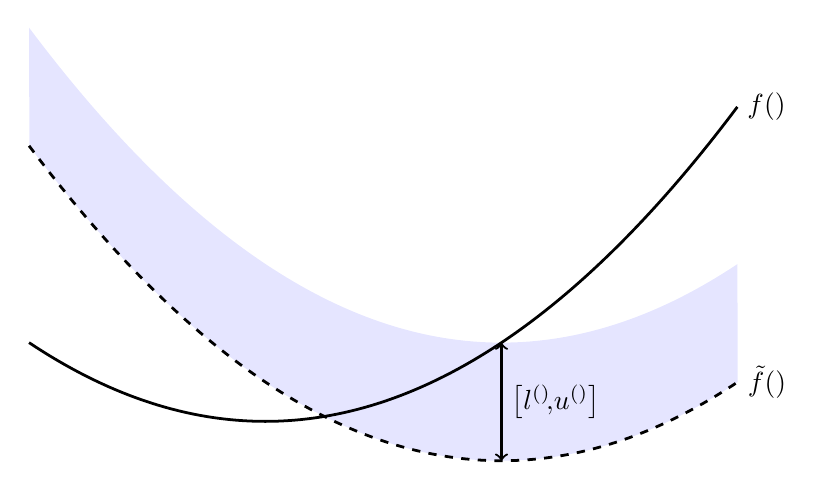
\begin{tikzpicture}[x=3cm, y=1cm]
  			% Filled band around the quadratic curve with different boundary curves
			\fill[blue!10] 
			(-1, 5) -- plot[domain=-2:1, samples=100] ({\x+1}, {\x*\x + 1}) -- 
			plot[domain=1:-2, samples=100] ({\x+1}, {\x*\x - 0.5}) -- cycle;
  			\node[anchor=west] at (2, 4) {$f(\weights)$};
  			\draw[line width=1, domain=-2:1, samples=100,dashed] plot  ({\x+1}, {\x*\x -0.5}) node[right] {$\tilde{f}(\weights)$};
   			\draw[line width=1, domain=-1:2, samples=100] plot ({\x}, {\x*\x});
  			\draw[<->, thick] (1, -0.5) -- (1, 1) node[midway, right] {$\big[ l^{(\weights)}\!,\!u^{(\weights)} \big]$};
			\end{tikzpicture}
		\caption{\gls{ml} methods learn \glspl{modelparam} $\weights$ by using some estimate of $f(\weights)$ for 
			the ultimate performance criterion $\bar{f}(\weights)$. Using a \gls{probmodel}, one can use $f(\weights)$ to 
			construct confidence intervals $\big[ l^{(\weights)},  u^{(\weights)} \big]$, which contain $\bar{f}(\weights)$  
			with high \gls{probability}. The best plausible performance \gls{measure} for a specific choice $\weights$ of \glspl{modelparam} 
			is $\tilde{f}(\weights) \defeq l^{(\weights)}$. \label{fig_optimism_dict}} 
			\end{center}
		\end{figure}
		See also: \gls{objfunc}, \gls{ucb}, \gls{optmethod}, \gls{gdmethod}.},
	first={optimism in the face of uncertainty},
	text={optimism in the face of uncertainty} 
}

\newglossaryentry{flnetwork}
{name={federated learning network (FL network)},
	description={An \gls{fl} network\index{federated learning network (FL network)} is a 
		mathematical model for a \gls{flsystem} that consists of interconnected 
		\glspl{device}. These \glspl{device} are represented by the nodes $\nodes$ 
		of an undirected weighted \gls{graph}
		\[
			\graph = (\nodes,\edges,\mA).
		\]
		An edge $\{\nodeidx,\nodeidx'\} \in \edges$ indicates collaborations 
		between two \glspl{device} $\nodeidx, \nodeidx' \in \nodes$. 
		The \glspl{edgeweight} $\edgeweight_{\nodeidx,\nodeidx'} > 0$ 
		quantify the extent of collaborations, which may be related to a 
		communication link capacity, statistical similarity between 
		\glspl{localdataset}, or both. Each \gls{device} $\nodeidx \in \nodes$ 
		has potentially access to a \gls{localdataset} $\localdataset{\nodeidx}$ and 
		might train a \gls{localmodel} $\localmodel{\nodeidx}$, e.g., using 
		\gls{erm}-based methods. Many popular \gls{fl} methods are obtained by 
		coupling the \gls{training} of these \glspl{localmodel} across the edges of the 
		\gls{fl} network \cite{JungFLBook}. This coupling can be implemented in different ways, 
		e.g., using a \gls{penaltyterm} that enforces similarity between the \glspl{modelparam} 
		of neighboring \glspl{device}, or using the \glspl{prediction} of neighboring 
		\glspl{device} to augment the \glspl{localdataset}.
		Fig.\ \ref{fig_fl_network_dict} illustrates an \gls{fl} network with four \glspl{device}.
		\begin{figure}[H]
		\centering
		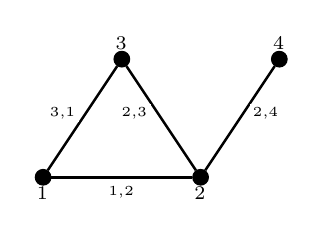
\begin{tikzpicture}[
			scale=1,
			node/.style={circle, draw=black, fill=black, inner sep=2pt},
			edge/.style={line width=0.9pt},
			wlab/.style={fill=white, inner sep=1pt, font=\scriptsize}
			]
			% Nodes
			\node[node] (v1) at (0,0) {};
			\node[node] (v2) at (2,0) {};
			\node[node] (v3) at (1,1.5) {};
			\node[node] (v4) at (3,1.5) {};
			% Labels
			\node[anchor=north] at (v1) {$\nodeidx_1$};
			\node[anchor=north] at (v2) {$\nodeidx_2$};
			\node[anchor=south] at (v3) {$\nodeidx_3$};
			\node[anchor=south] at (v4) {$\nodeidx_4$};
			% Undirected weighted edges + weight labels next to edges
			\draw[edge] (v1) -- node[wlab, pos=0.5, below, yshift=-2pt] {$\edgeweight_{1,2}$} (v2);
			\draw[edge] (v2) -- node[wlab, pos=0.55, left,  xshift=-2pt] {$\edgeweight_{2,3}$} (v3);
			\draw[edge] (v3) -- node[wlab, pos=0.45, left,  xshift=-2pt] {$\edgeweight_{3,1}$} (v1);
			\draw[edge] (v2) -- node[wlab, pos=0.55, right, xshift=2pt] {$\edgeweight_{2,4}$} (v4);
			\end{tikzpicture}
		\caption{An \gls{fl} network with nodes $\nodes=\{\nodeidx_1,\nodeidx_2,\nodeidx_3,\nodeidx_4\}$ 
			representing four \glspl{device} of an \gls{flsystem}. \label{fig_fl_network_dict}}
		\end{figure}
		The \gls{fl} network specifies which \glspl{device} can interact and to what extent. 
	    	\\
		See also: \gls{fl}, \gls{device}, \gls{graph}, \gls{gtvmin}.},
	first={federated learning network (FL network)},
	text={FL network},
	plural={FL networks}, 
	firstplural={federated learning networks (FL networks)}
}

\newglossaryentry{explanation}
{name={explanation},
	description={One approach to enhance the \gls{transparency} of an \gls{ml} method for its human user 
		is to provide an explanation\index{explanation} alongside the \glspl{prediction} delivered 
		by the method. Explanations can take different forms. For instance, they may 
        		consist of human-readable text or quantitative indicators, such as \gls{feature} 
        		importance scores for the individual \glspl{feature} of a given \gls{datapoint}~\cite{Molnar2019}. 
	   	Alternatively, explanations can be visual—for example, intensity \glspl{map} that highlight 
	   	image regions that drive the \gls{prediction} \cite{GradCamPaper}. 
       		Fig.\ \ref{fig_explanation_dict} illustrates two types of explanations. The first 
       		is a local linear approximation $g(\featurevec)$ of a nonlinear trained \gls{model} 
       		$\learnthypothesis(\featurevec)$ around a specific \gls{featurevec} $\featurevec'$, 
       		as used in the method \gls{lime}. 
        		The second form of explanation depicted in the figure is a sparse set of \glspl{prediction} 
       		$\learnthypothesis(\featurevec^{(1)}), \learnthypothesis(\featurevec^{(2)}), \learnthypothesis(\featurevec^{(3)})$ 
       		at selected \glspl{featurevec}, offering concrete reference points for the user. 
	 	\begin{figure}[H]
	   		\begin{center}
	 		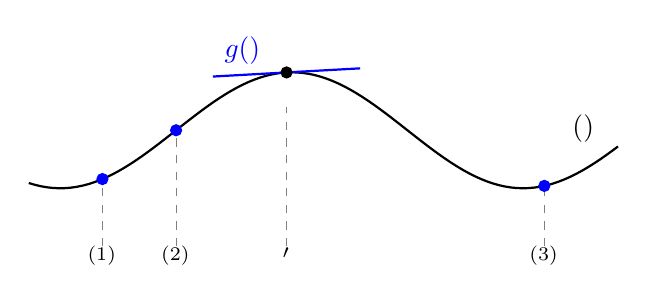
\begin{tikzpicture}[x=0.5cm]
	 		\begin{axis}[
	 			hide axis,
	 			xmin=-3, xmax=6,
	 			ymin=0, ymax=6,
	 			domain=0:6,
	 			samples=100,
	 			width=10cm,
	 			height=6cm,
	 			clip=false
	 		   ]
	 		% Original nonlinear function h(x)
			\addplot[thick, domain=-2:6] {2 + sin(deg(x))} 
	   		node[pos=0.9, above right, yshift=10pt] {$\learnthypothesis(\featurevec)$};
	 		% Tangent line as local linear approximation at x = 1.5
	 		% h(3) = 2 + sin(3), h'(3) = cos(3)
	 		\addplot[blue, thick, domain=0.5:2.5] 
	 		{2 + sin(deg(1.5)) + cos(deg(1.5))*(x - 1.5)}
	 		node[pos=0.2, above] {$g(\featurevec)$};
	 		% Mark point of approximation
	 		\addplot[mark=*] coordinates {(1.5, {2 + sin(deg(1.5))})};
	 		    % Vertical dashed line (ruler) at x = 1.5
			\addplot[dashed, gray] coordinates {(1.5,0) (1.5,2.4)};
	 		\node at (axis cs:1.5, -0.2) {$\featurevec'$};
	      		% add function values for finite set of featurevecs
	       		\addplot[mark=*,blue] coordinates {(-1, {2 + sin(deg(-1))})};
	       		\addplot[dashed, gray] coordinates {(-1,0) (-1,{2 + sin(deg(-1))})};
	       		\node at (axis cs:-1, -0.2) {$\featurevec^{(1)}$};
	 	   	\addplot[mark=*,blue] coordinates {(0, {2 + sin(deg(0))})};
	 	   	\addplot[dashed, gray] coordinates {(0,0) (0,{2 + sin(deg(0))})};
	 	   	\node at (axis cs:0, -0.2) {$\featurevec^{(2)}$};
	 	   	\addplot[mark=*,blue] coordinates {(5, {2 + sin(deg(5))})};
	 	   	\addplot[dashed, gray] coordinates {(5,0) (5,{2 + sin(deg(5))})};
	 	   	\node at (axis cs:5, -0.2) {$\featurevec^{(3)}$};
			% 		    % Plot the two points
			% 		    % Coordinates of the two points
			% 		\pgfmathsetmacro{\xA}{-1.5}
			% 		\pgfmathsetmacro{\xB}{3}
			% 		\pgfmathsetmacro{\yA}{2 + sin(deg(\xA))}
			% 		\pgfmathsetmacro{\yB}{2 + sin(deg(\xB))}
	 		\end{axis}
			% 	\vspace*{-10mm}
			\end{tikzpicture}
	 	\end{center}
	 	\caption{A trained \gls{model} $\learnthypothesis(\featurevec)$ can be explained 
	     		locally at some point $\featurevec'$ by a linear approximation $g(\featurevec)$. 
	     		For a \gls{differentiable} $\learnthypothesis(\featurevec)$, this approximation is 
	     		determined by the \gls{gradient} $\nabla \learnthypothesis(\featurevec')$. Another 
	     		form of explanation could be the \gls{function} values $\learnthypothesis\big(\featurevec^{(\sampleidx)} \big)$ 
	     		for $\sampleidx=1, \,2, \,3$. 
			\label{fig_explanation_dict}}
	 	\end{figure} 
		See also: \gls{ml}, \gls{prediction}, \gls{feature}, \gls{datapoint}, \gls{classification}.},
	first={explanation},
	plural={explanations},
	text={explanation} 
}

\newglossaryentry{risk}
{name={risk},
	description={Consider\index{risk} a \gls{hypothesis} $\hypothesis$ used to predict the \gls{label} 
		$\truelabel$ of a \gls{datapoint} based on its \glspl{feature} $\featurevec$. We measure 
		the quality of a particular \gls{prediction} using a \gls{lossfunc} $\lossfunc{(\featurevec,\truelabel)}{\hypothesis}$. 
		If we interpret \glspl{datapoint} as the \glspl{realization} of \gls{iid} \glspl{rv}, 
		the $\lossfunc{(\featurevec,\truelabel)}{\hypothesis}$ also becomes the \gls{realization} 
		of an \gls{rv}. The \gls{iidasspt} allows us to define the risk of a \gls{hypothesis} 
		as the expected \gls{loss} $\expect \big\{\lossfunc{(\featurevec,\truelabel)}{\hypothesis} \big\}$. 
		Note that the risk of $\hypothesis$ depends on both the specific choice for the \gls{lossfunc} and the 
		\gls{probdist} of the \glspl{datapoint}.
					\\ 
		See also: \gls{iid} \gls{rv}, \gls{iidasspt}, \gls{loss}, \gls{probdist}.},
	first={risk},
	text={risk} 
}

\newglossaryentry{actfun}
{name={activation function},
	description={Each\index{activation function} artificial neuron within an \gls{ann} is 
		assigned an \gls{activation} \gls{function} $\actfun(\cdot)$ that maps a weighted 
		combination of the neuron inputs $\feature_{1}, \,\ldots, \,\feature_{\nrfeatures}$ 
		to a single \gls{output} value $a = \actfun\big(\weight_{1} \feature_{1}+\ldots+\weight_{\nrfeatures} \feature_{\nrfeatures} \big)$. 
		Note that each neuron is parameterized by the \glspl{weight} $\weight_{1}, \,\ldots, \,\weight_{\nrfeatures}$.
					\\ 
		See also: \gls{ann}, \gls{activation}, \gls{relu}.},
	first={activation function},
	text={activation function} 
}

\newglossaryentry{distributedalgorithm}
{name={distributed algorithm},
	description={A\index{distributed algorithm} distributed \gls{algorithm} is an \gls{algorithm} designed for 
		a special type of computer, i.e., a collection of interconnected computing \glspl{device} (or nodes). 
		These \glspl{device} communicate and coordinate their local computations by exchanging 
		messages over a network \cite{IntroDistAlg}, \cite{ParallelDistrBook}. Unlike a classical \gls{algorithm}, 
		which is implemented on a single \gls{device}, a distributed \gls{algorithm} is 
		executed concurrently on multiple \glspl{device} with computational capabilities. 
		Similar to a classical \gls{algorithm}, a distributed \gls{algorithm} can be modeled as a 
		set of potential executions. However, each execution in the distributed setting involves 
		both local computations and message-passing \glspl{event}. A generic execution might look as 
		follows:
		\[
		\begin{array}{l}
			\text{Node 1: } {\rm input}_1, \,s_1^{(1)}, \,s_2^{(1)}, \,\ldots, \,s_{T_1}^{(1)}, \,{\rm \gls{output}}_1; \\
			\text{Node 2: } {\rm input}_2, \,s_1^{(2)}, \,s_2^{(2)}, \,\ldots, \,s_{T_2}^{(2)}, \,{\rm \gls{output}}_2; \\
			\quad \vdots \\
			\text{Node N: } {\rm input}_N, \,s_1^{(N)}, \,s_2^{(N)}, \,\ldots, \,s_{T_N}^{(N)}, \,{\rm \gls{output}}_N.
		\end{array}
		\]
		Each \gls{device} $\nodeidx$ starts from its own local input and performs a \gls{sequence} of 
		intermediate computations $s_{\iteridx}^{(\nodeidx)}$ at discrete-time instants $\iteridx = 1, \,\dots, \,T_\nodeidx$. 
		These computations may depend on both the previous local computations at the \gls{device} 
		and the messages received from other \glspl{device}. One important application of distributed 
		\glspl{algorithm} is in \gls{fl} where a network of \glspl{device} collaboratively trains a personal \gls{model} 
		for each \gls{device}. 
					\\ 
		See also: \gls{algorithm}, \gls{device}, \gls{event}, \gls{fl}, \gls{model}.},
	first={distributed algorithm}, 
	text={distributed algorithm}
}

\newglossaryentry{algorithm}
{name={algorithm},
 	description={An\index{algorithm} algorithm is a precise, step-by-step specification for 
  		producing an \gls{output} from a given input within a finite number of well-defined 
		computational steps \cite{Cormen:2022aa}. For example, a \gls{gdmethod} for \gls{linreg} 
		is an algorithm that explicitly describes how to map a given \gls{trainset} 
		into \glspl{modelparam} through a sequence of \glspl{gradstep}. The precise form of 
		an algorithm depends on the available computational infrastructure. For example, if 
		this infrastructure allows us to compute an \gls{inverse}, then we can 
		define a \gls{linreg} algorithm using the \gls{normalequations}. In contrast, if 
		the computational infrastructure only allows basic arithmetic operations (i.e., multiplication and addition), 
		the \gls{normalequations} need to be somehow translated into a sequence of arithmetic 
		operations (e.g., as in \glspl{gdmethod}). 
		To study algorithms rigorously, we can represent (or approximate) them by different 
		mathematical structures \cite{Sipser2013}. One approach is to represent an algorithm 
		as a collection of possible executions. Each individual execution is then a 
		\gls{sequence} of the following form: $${\rm input}, \,s_1, \,s_2, \,\ldots, \,s_T, \,{\rm \gls{output}}.$$ 
		This sequence starts from an input and progresses via intermediate steps until an 
		\gls{output} is delivered. Crucially, an algorithm encompasses more than just a mapping 
		from input to \gls{output}; it also includes intermediate computational 
     		steps $s_1, \,\ldots, \,s_T$.
				\\ 
		See also: \gls{output}, \gls{linreg}, \gls{trainset}, \gls{modelparam}, \gls{gradstep}, \gls{model}, \gls{stochastic}.},
	first={algorithm},
	plural={algorithms},
	text={algorithm} 
}

\newglossaryentry{stochalgorithm}
{name={stochastic algorithm},
	description={A\index{stochastic algorithm} \gls{stochastic} \gls{algorithm} uses a random mechanism 
		during its execution. For example, \gls{stochGD} uses a randomly selected subset of \glspl{datapoint} 
		to compute an approximation for the \gls{gradient} of an \gls{objfunc}. We can represent a 
		\gls{stochastic} \gls{algorithm} by a \glspl{stochproc}, i.e., the possible execution \gls{sequence} is the possible \glspl{outcome} of 
		a \gls{randomexperiment} \cite{BertsekasProb}, \cite{RandomizedAlgos}, \cite{Gallager13}.		
		\\ 
		See also: \gls{stochastic}, \gls{algorithm}, \gls{stochGD}, \gls{datapoint}, \gls{gradient}, \gls{objfunc}, \gls{stochproc}, 
		\gls{randomexperiment}, \gls{optmethod}, \gls{gdmethod}. },
	first={stochastic algorithm},
	text={stochastic algorithm},
	plural={stochastic algorithms},
	firstplural={stochastic algorithms}
}

\newglossaryentry{batchlearning}
{name={batch learning},
	description={In \gls{batch} learning\index{batch learning} (also known as offline learning), the \gls{ml} \gls{model} 
		is trained on the entire \gls{dataset} in a single \gls{training} iteration, instead of updating it incrementally as \gls{data} arrive. 
		All available \gls{data} are inputted into a learning \gls{algorithm}, resulting in a \gls{model} that can make \glspl{prediction}. 
		Since these \glspl{dataset} tend to be large, \gls{training} is computationally expensive and time-consuming, 
		so it is typically performed offline. After learning, the \gls{model} will be static and will not adapt to new \gls{data} automatically. 
		Updating the \gls{model} with new information requires retraining the \gls{model} entirely. Once the \gls{model} has been trained, 
		it is launched into production where it cannot be updated. \Gls{training} a \gls{model} can take many hours, so many \glspl{model} in production 
		settings are updated cyclically on a periodic schedule when the \gls{data} distribution is stable. For example, a retail analytics team 
		could retrain their demand forecast \gls{model} every Sunday using the previous week's sales \gls{data} to predict next week's demand. 
		If a system needs to be constantly updated to rapidly changing \gls{data}, such as in stock price \gls{prediction}, a more adaptable solution 
		such as \gls{onlinelearning} is necessary.
		\\
		See also: \gls{batch}, \gls{model}, \gls{dataset}, \gls{onlinelearning}. },
	first={batch learning}, 
	text={batch learning}
}

\newglossaryentry{onlinelearning}
{name={online learning},
	description={Some \gls{ml} methods\index{online learning} are designed to 
	    	process \gls{data} in a sequential manner, updating their \glspl{modelparam} 
		one at a time, as new \glspl{datapoint} become available. A typical example 
		is time-series \gls{data}, such as daily \gls{minimum} and \gls{maximum} 
		temperatures recorded by an \gls{fmi} weather station. These values form 
		a chronological sequence of observations. During each time step $\timeidx$, 
		online learning methods update (or refine) the current \gls{hypothesis} 
		$\hypothesis^{(\timeidx)}$ (or \glspl{modelparam} $\weights^{(\timeidx)}$) 
		based on the newly observed \gls{datapoint} $\datapoint^{(\timeidx)}$. 
		\\ 
		See also: \gls{onlineGD}, \gls{onlinealgorithm}. },
	first={online learning},
	text={online learning} 
}

\newglossaryentry{onlinealgorithm}
{name={online algorithm},
	description={An\index{online algorithm} online \gls{algorithm} processes input \gls{data} incrementally, 
		receiving \glspl{datapoint} sequentially and making decisions or producing \glspl{output} (or decisions) immediately 
		without having access to the entire input in advance \cite{PredictionLearningGames}, \cite{HazanOCO}. 
		Unlike an offline \gls{algorithm}, which has the entire input available from the start, an online \gls{algorithm} 
		must handle \gls{uncertainty} about future inputs and cannot revise past decisions. Similar to an 
		offline \gls{algorithm}, we represent an online \gls{algorithm} formally as a collection of possible 
		executions. However, the execution \gls{sequence} for an online \gls{algorithm} has a distinct structure as follows:
		$${\rm in}_{1}, \,s_1, \,{\rm out}_{1}, \,{\rm in}_{2}, \,s_2, \,{\rm out}_{2}, \,\ldots, \,{\rm in}_{T}, \,s_T, \,{\rm out}_{T}.$$ 
		Each execution begins from an initial state (i.e., \(\text{in}_{1}\)) and proceeds through alternating 
		computational steps, \glspl{output} (or decisions), and inputs. Specifically, at step \(\iteridx\), 
		the \gls{algorithm} performs a computational step \(s_{\iteridx}\), generates an \gls{output} \(\text{out}_{\iteridx}\), 
		and then subsequently receives the next input (\gls{datapoint}) \(\text{in}_{\iteridx+1}\). A 
		notable example of an online \gls{algorithm} in \gls{ml} is \gls{onlineGD}, which incrementally 
		updates \glspl{modelparam} as new \glspl{datapoint} arrive. 
					\\ 
		See also: \gls{algorithm}, \gls{data}, \gls{datapoint}, \gls{uncertainty}, \gls{ml}, \gls{onlineGD}, \gls{modelparam}, \gls{onlinelearning}.},
	first={online algorithm},
	text={online algorithm} 
}

\newglossaryentry{sensattr}
{name={sensitive attribute},
	description={\gls{ml}\index{sensitive attribute} revolves around learning a \gls{hypothesis} \gls{map} that allows 
		us to predict the \gls{label} of a \gls{datapoint} from its \glspl{feature}. In some 
		applications, we must ensure that the \gls{output} delivered by an \gls{mlsystem} does 
		not allow us to infer sensitive attributes of a \gls{datapoint}. Which part 
		of a \gls{datapoint} is considered a sensitive attribute is a design 
		choice that varies across different application domains.
					\\ 
		See also: \gls{ml}, \gls{hypothesis}, \gls{map}, \gls{label}, \gls{datapoint}, \gls{feature}.},
	first={sensitive attribute},
	plural={sensitive attributes},
	firstplural={sensitive attributes},
	text={sensitive attribute} 
}

\newglossaryentry{sbm}
{name={stochastic block model (SBM)},
	description={The\index{stochastic block model (SBM)} SBM \cite{holland1983stochastic} is a 
		probabilistic generative \gls{model} for an \gls{undirectedgraph} $\graph = \big( \nodes, \edges \big)$ 
		with a given set of nodes $\nodes$ \cite{AbbeSBM2018}. In its most basic variant, 
		the SBM generates a \gls{graph} by first randomly assigning each node $\nodeidx \in \nodes$ to 
		a \gls{cluster} index $\clusteridx_{\nodeidx} \in \{1, \,\ldots, \,\nrcluster\}$. A pair of different nodes in the 
		\gls{graph} is \gls{connected} by an edge with \gls{probability} $p_{\nodeidx,\nodeidx'}$ that depends 
		solely on the \glspl{label} $\clusteridx_{\nodeidx}, \clusteridx_{\nodeidx'}$. 
		The presence of edges between different pairs of 
		nodes is statistically independent.
					\\ 
		See also: \gls{model}, \gls{graph}, \gls{cluster}, \gls{probability}, \gls{label}. },
	first={stochastic block model (SBM)},
	text={SBM} 
}

\newglossaryentry{deepnet}
{name={deep net},
	description={A\index{deep net} deep net is an \gls{ann} with a 
	    	(relatively) large number of hidden \glspl{layer}. \Gls{deeplearning} 
		is an umbrella term for \gls{ml} methods that use a deep 
		net as their \gls{model} \cite{Goodfellow-et-al-2016}.
				\\ 
		See also: \gls{ann}, \gls{layer}, \gls{deeplearning}, \gls{model}, \gls{llm}.},
	first={deep net},
	plural={deep nets},
	firstplural={deep nets},
	text={deep net} 
}

\newglossaryentry{baseline}
{name={baseline},
	description={Consider\index{baseline} some \gls{ml} method that produces a learned 
    		\gls{hypothesis} (or trained \gls{model}) $\learnthypothesis \in \hypospace$. We evaluate the quality of a trained \gls{model} 
    		by computing the average \gls{loss} on a \gls{testset}. But how can we assess 
    		whether the resulting \gls{testset} performance is sufficiently good? How can we 
    		determine if the trained \gls{model} performs close to optimal such that there is little point 
   		in investing more resources (for \gls{data} collection or computation) to improve it? 
    		To this end, it is useful to have a reference (or baseline) level against which 
    		we can compare the performance of the trained \gls{model}. \\
		Such a reference value might be obtained from human performance, e.g., the misclassification rate of dermatologists 
    		who diagnose cancer from visual inspection of skin \cite{SkinHumanAI}. Another source for a baseline is an existing, 
    		but for some reason unsuitable, \gls{ml} method. For example, the existing \gls{ml} method 
    		might be computationally too expensive for the intended \gls{ml} application. 
    		Nevertheless, its \gls{testset} error can still serve as a baseline. Another, somewhat more principled, 
    		approach to constructing a baseline is via a \gls{probmodel}. In many cases, given a \gls{probmodel} $p(\featurevec,\truelabel)$,  
    		we can precisely determine the \gls{minimum} achievable \gls{risk} among any \glspl{hypothesis}
    		(not even required to belong to the \gls{hypospace} $\hypospace$) \cite{LC}. \\
    		This \gls{minimum} achievable \gls{risk} (referred to as the \gls{bayesrisk}) is the \gls{risk} 
    		of the \gls{bayesestimator} for the \gls{label} $\truelabel$ of a \gls{datapoint}, given
    		its \glspl{feature} $\featurevec$. Note that, for a given choice of \gls{lossfunc}, the 
    		\gls{bayesestimator} (if it exists) is completely determined by the \gls{probdist} 
		$\probdist$ \cite[Ch. 4]{LC}. However, computing the \gls{bayesestimator} 
		and \gls{bayesrisk} presents two main challenges. First, the \gls{probdist} 
		$\probdist$ is unknown and must be estimated from observed \gls{data}. Second, even if $\probdist$ 
		were known, computing the \gls{bayesrisk} exactly may be computationally 
		infeasible \cite{cooper1990computational}. 
		A widely used \gls{probmodel} is the \gls{mvndist} $\pair{\featurevec}{\truelabel} \sim \mathcal{N}({\bm \mu},{\bm \Sigma})$ 
		for \glspl{datapoint} characterized by numeric \glspl{feature} and \glspl{label}.
		Here, for the \gls{sqerrloss}, the \gls{bayesestimator} is given by the \gls{posterior} 
		\gls{mean} $\mu_{\truelabel|\featurevec}$ of the \gls{label} $\truelabel$, given the 
		\glspl{feature} $\featurevec$ \cite{GrayProbBook}, \cite{LC}. The corresponding \gls{bayesrisk} 
		is given by the \gls{posterior} \gls{variance} 
		$\sigma^{2}_{\truelabel|\featurevec}$ (see Fig. \ref{fig_post_baseline_dict}).
		\begin{figure}[H]
		\begin{center}
		\begin{tikzpicture}
			% Axes
			\draw[->] (-1,0) -- (7,0) node[right] {$\truelabel$}; % x-axis
			% Gaussian distribution centered at 3 with variance 1
			\draw[thick,domain=-1:7,smooth,variable=\x] 
			plot ({\x}, {2*exp(-0.5*((\x-3)^2))});
			% Dashed line indicating the mean of the Gaussian
			\draw[dashed] (3,0) -- (3,2.5);
			\node[anchor=south] at ([yshift=-5pt] 3,2.5) {\small $\mu_{\truelabel|\featurevec}$};
			% Double arrow indicating the variance
			\draw[<->,thick] (3-1,1) -- (3+1,1.0);
			\node[anchor=west] at ([yshift=2pt] 3,1.2) {\small $\sigma_{\truelabel|\featurevec}$};
			% Posterior variance label
			%\node[anchor=south east] at (3-0.5,1.8) {\small Posterior Variance};
			% x-axis marks with crosses
			% x-axis marks with crosses
  			\foreach \x in {0.5} {
			\node[red] at (\x, 0) {\bf \large $\times$};
 			}
  			% h(x) label for the first cross
  			\node[anchor=north] at (0.5,-0.2) {\small $\learnthypothesis(\featurevec)$};
		\end{tikzpicture}
		\end{center}
		\caption{If the \glspl{feature} and the \gls{label} of a \gls{datapoint} are drawn 
			from a \gls{mvndist}, we can achieve the \gls{minimum} \gls{risk} (under \gls{sqerrloss}) 
			by using the \gls{bayesestimator} $\mu_{\truelabel|\featurevec}$ 
			to predict the \gls{label} $\truelabel$ of a \gls{datapoint} with \glspl{feature} $\featurevec$. The corresponding 
			\gls{minimum} \gls{risk} is given by the \gls{posterior} \gls{variance} $\sigma^{2}_{\truelabel|\featurevec}$. We can use 
			this quantity as a baseline for the average \gls{loss} of a trained \gls{model} $\learnthypothesis$. \label{fig_post_baseline_dict}}
		\end{figure}
		See also: \gls{bayesrisk}, \gls{bayesestimator}.},
    first={baseline},
    text={baseline}
}

\newglossaryentry{kfoldcv}
{name={$k$-fold cross-validation ($k$-fold CV)},
sort={k-fold CV},
	description={A $k$-fold CV is a method\index{$k$-fold cross-validation ($k$-fold CV)} for evaluating the 
 		\gls{gengap} of an \gls{erm}-based \gls{ml} method. The idea is to divide a \gls{dataset} 
 		$\dataset$ evenly into $k$ subsets (or folds) $\dataset^{(1)},\,\ldots,\,\dataset^{(k)}$.
		\begin{figure}[H]
		\centering
			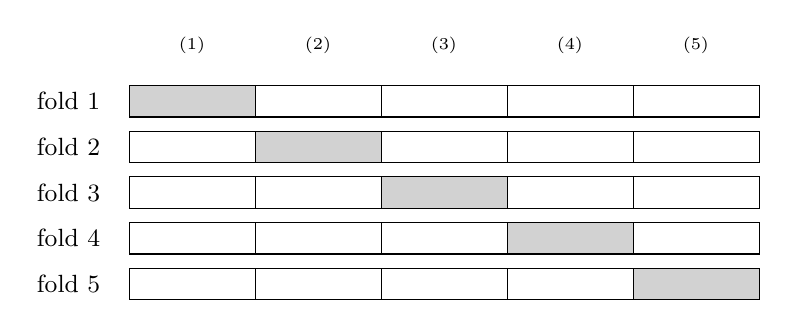
\begin{tikzpicture}[font=\small]
				\def\k{5}          % number of folds
				\def\cellw{1.6}    % width of one segment
				\def\cellh{0.40}   % height of one segment
				\def\gap{0.18}     % vertical gap between rows
				% rows: i = 1..k; columns: j = 1..k
				\foreach \i in {1,...,\k} {
					% row baseline y
					\pgfmathsetmacro{\y}{-(\i-1)*(\cellh+\gap)}
					% row label
					\node[anchor=east] at (-0.25,\y+0.5*\cellh) {fold \i};
					% draw k equal segments; shade the \i-th as validation
					\foreach \j in {1,...,\k} {
						\pgfmathsetmacro{\x}{(\j-1)*\cellw}
						\ifnum\i=\j
						\fill[gray!35] (\x,\y) rectangle ++(\cellw,\cellh);
						\draw (\x,\y) rectangle ++(\cellw,\cellh);
						\else
						\draw (\x,\y) rectangle ++(\cellw,\cellh);
						\fi
					}
				}
				% add labels D^{(j)} above the columns
				\foreach \j in {1,...,\k} {
					\pgfmathsetmacro{\x}{(\j-1)*\cellw + 0.5*\cellw}
					\node[anchor=south] at (\x,\cellh+0.2) {$\dataset^{(\j)}$};
				}
			\end{tikzpicture}
		\caption{In $k$-fold CV, the available \gls{dataset} $\dataset$ is 
			evenly divided into $k$ folds $\dataset^{(1)},\,\ldots,\,\dataset^{(k)}$. Each fold is used once as a 
			\gls{valset}, while the remaining $k-1$ folds form the \gls{trainset}.		
			\label{fig_kfoldcv_dict}}
		\end{figure} 
		For each fold $\foldidx = 1, \,\ldots, \,k$, we train the \gls{model} on the 
		union of all folds except $\dataset^{(\foldidx)}$ and validate it on 
		$\dataset^{(\foldidx)}$. The overall performance is obtained by averaging 
		the \gls{validation} results across all $k$ folds.
		\\
		See also: \gls{validation}, \gls{valerr}.},
	first={$k$-fold cross-validation ($k$-fold CV)},
	text={$k$-fold CV} 
}

\newglossaryentry{loo}
{name={leave-one-out cross-validation (LOO-CV)},
	description={LOO-CV is a special case\index{leave-one-out cross-validation (LOO-CV)} 
		of \gls{kfoldcv} where the \gls{valset} is of size one, i.e., a single \gls{datapoint}. 
		\\
		% Error 
		See also: \gls{kfoldcv}, \gls{validation}, \gls{valerr}.},
	first={leave-one-out cross-validation (LOO-CV)},
	text={LOO-CV}
}

\newglossaryentry{nestedcv}
{name={nested cross-validation (nested CV)},
	description={Nested CV\index{nested cross-validation (nested CV)} is a method 
		of extending the \gls{kfoldcv} from training and \glspl{valset} to also cover the \gls{testset}. 
		Instead of simply choosing a single \gls{testset} from the \gls{data}, two loops are run, i.e., 
		the outer and the inner loop. The outer loop uses \gls{kfoldcv} to separate a \gls{testset} 
		from the \gls{data}, and the inner loop again uses \gls{kfoldcv} to separate the remaining data 
		into training and \glspl{valset}. Doing this decreases the \gls{variance} and \gls{bias} in the results. 
		\\
		% Todo: Figure pending
		% Todo: Changing k-folds to k-fold and n-fold.
		See also: \gls{kfoldcv}, \gls{loo}, \gls{validation}, \gls{valerr}.},
	first={nested cross-validation (nested CV)},
	text={nested CV},
	firstplural={nested cross-validations (nested CVs)},
	plural={nested CVs}
}

\newglossaryentry{spectrogram}
{name={spectrogram},
	description={A\index{spectrogram} spectrogram represents the time-frequency distribution of the energy of a time signal $x(t)$.  
		Intuitively, it quantifies the amount of signal energy present within a specific time segment 
		$[t_{1},t_{2}] \subseteq \mathbb{R}$ and frequency interval $[f_{1},f_{2}]\subseteq \mathbb{R}$. 
		Formally, the spectrogram of a signal is defined as the squared magnitude of its 
		short-time Fourier transform (STFT) \cite{cohen1995time}.
        		Fig. \ref{fig:spectrogram_dict} depicts a time signal along with its spectrogram. 
		\begin{figure}[H]
			\centering
			\includegraphics[width=0.8\textwidth]{assets/spectrogram.png}
			\begin{minipage}{\textwidth}
				\vspace{3ex}
				\centering
				{\selectfont (a) \hspace{10em} (b)}
			\end{minipage}
			\caption{(a) A time signal consisting of two modulated \gls{gaussian} pulses. (b) An intensity 
			plot of the spectrogram.
			\label{fig:spectrogram_dict}}
		\end{figure}
        		The intensity plot of its spectrogram can serve as an image of a signal. A 
		simple recipe for audio signal \gls{classification} is to feed this signal image 
		into \glspl{deepnet} originally developed for image \gls{classification} and object detection \cite{Li:2022aa}. 
		It is worth noting that, beyond the spectrogram, several alternative representations exist 
		for the time-frequency distribution of signal energy \cite{TimeFrequencyAnalysisBoashash}, \cite{MallatBook}.
					\\ 
		See also: \gls{classification}, \gls{deepnet}.}, 
	first={spectrogram},
	text={spectrogram} 
}

\newglossaryentry{graphclustering}
{name={graph clustering},
	description={\Gls{graph} \gls{clustering}\index{graph clustering} aims to 
		cluster \glspl{datapoint} that are represented as the nodes 
		of a \gls{graph} $\graph$. The edges of $\graph$ represent 
		pairwise similarities between \glspl{datapoint}. We can sometimes
		quantify the extent of these similarities by an \gls{edgeweight} \cite{FlowSpecClustering2021}, \cite{Luxburg2007}.
					\\ 
		See also: \gls{graph}, \gls{clustering}, \gls{datapoint}, \gls{edgeweight}. }, 
	first={graph clustering},
	text={graph clustering} 
}

\newglossaryentry{specclustering}
{name={spectral clustering},
	description={Spectral \gls{clustering}\index{spectral clustering} is a particular instance of 
		\gls{graphclustering}, i.e., it clusters \glspl{datapoint} 
		represented as the nodes $\nodeidx=1, \,\ldots, \,\nrnodes$ of a \gls{graph} $\graph$. 
		Spectral \gls{clustering} uses the \glspl{eigenvector} of the \gls{LapMat} $\LapMat{\graph}$ 
		to construct \glspl{featurevec} $\featurevec^{(\nodeidx)} \in \mathbb{R}^{\nrfeatures}$ 
		for each node (i.e., for each \gls{datapoint}) $\nodeidx=1, \,\ldots, \,\nrnodes$. We can feed these \glspl{featurevec} 
		into \gls{euclidspace}-based \gls{clustering} methods, such as \gls{kmeans} 
		or \gls{softclustering} via \gls{gmm}. Roughly speaking, the \glspl{featurevec} of nodes 
		belonging to a well-connected subset (or \gls{cluster}) of nodes in $\graph$ are located 
		nearby in the \gls{euclidspace} $\mathbb{R}^{\nrfeatures}$ (see Fig. \ref{fig_lap_mtx_specclustering_dict}). 
		\begin{figure}[H]
			\begin{center}
				\begin{minipage}{0.4\textwidth}
			\begin{tikzpicture}
				% Define the style for filled nodes
				\begin{scope}[every node/.style={circle, fill=black, inner sep=0pt, minimum size=0.3cm}]
					% Define nodes
					\node (1) at (0,0) {};
					\node (2) [below left=of 1, xshift=-0.2cm, yshift=-1cm] {};
					\node (3) [below right=of 1, xshift=0.2cm, yshift=-1cm] {};
					\node (4) [below=of 1, yshift=0.5cm] {}; % Isolated node
				\end{scope}
				% Draw edges
				\draw (1) -- (2);
				\draw (1) -- (3);
				% Add labels (separate from filled nodes)
				\node[above=0.2cm] at (1) {$\nodeidx=1$};
				\node[left=0.3cm] at (2) {$2$};
				\node[right=0.3cm] at (3) {$3$};
				\node[below=0.2cm] at (4) {$4$};
				\node at (0,-4) {(a)};
			\end{tikzpicture}
				\end{minipage} 
				\hspace*{5mm}
				\begin{minipage}{0.4\textwidth}
					\begin{equation} 
						\LapMat{\graph}\!=\!
						\begin{pmatrix} 
							2 & -1 & -1 & 0 \\ 
							-1 & 1 & 0 & 0 \\  
							-1 & 0 & 1 & 0 \\ 
							0 & 0 & 0 & 0 
						\end{pmatrix}\!=\!\mathbf{V} {\bm \Lambda} \mathbf{V}\,^{T}  
						\nonumber
					\end{equation} 
					\begin{minipage}{\textwidth}
						\vspace{3ex}
						\centering
						{\selectfont (b)}
					\end{minipage}
				\end{minipage}
				\vspace*{20mm}\\
				\begin{minipage}{0.4\textwidth}
			\begin{tikzpicture}[scale=3]
%					% Axes
					\draw[->] (-0.2, 0) -- (1.2, 0) node[right] {$v^{(1)}_{\nodeidx}$};
					\draw[->] (0, -0.2) -- (0, 1.2) node[above] {$v^{(2)}_{\nodeidx}$};
%					
%					% Tailored tick marks and labels
%					\draw (0,0) node[below left] {$0$};
%					\draw (1/sqrt(3), 0) node[below] {$\frac{1}{\sqrt{3}}$} -- ++(0,0.05);
%					\draw (0, 1) node[left] {$1$} -- ++(0.05,0);
%					
%					Data points
					\filldraw[blue] (0.577, 0) circle (0.03cm) node[above right] {$\nodeidx=1,2,3$};
					\filldraw[blue] (0.577, 0) circle (0.03cm); % Second point overlaps
					\filldraw[blue] (0.577, 0) circle (0.03cm); % Third point overlaps
					\filldraw[red] (0, 1) circle (0.03cm) node[above right] {$4$};
%					% Grid for reference
%					\draw[dashed, gray] (1/sqrt(3), 0) -- (1/sqrt(3), 1);
%					\draw[dashed, gray] (0, 1) -- (1, 1);
					\node at (0.5,-0.5) {(c)};
			\end{tikzpicture}
				\end{minipage} 
    				\begin{minipage}{0.4\textwidth}
					\begin{align}
					& \mathbf{V} = \big( \vv^{(1)},\vv^{(2)},\vv^{(3)},\vv^{(4)} \big) \nonumber \\
					&	\mathbf{v}^{(1)}\!=\!\frac{1}{\sqrt{3}} \begin{pmatrix} 1 \\ 1 \\ 1 \\ 0 \end{pmatrix}, \,
					\mathbf{v}^{(2)}\!=\!\begin{pmatrix} 0 \\ 0 \\ 0 \\ 1 \end{pmatrix} \nonumber 
					\end{align}
					\begin{minipage}{\textwidth}
						\vspace{3ex}
						\centering
						{\selectfont (d)}
					\end{minipage}
				\end{minipage} 
				\caption{\label{fig_lap_mtx_specclustering_dict} (a) An \gls{undirectedgraph} 
					$\graph$ with four nodes $\nodeidx=1,\,2,\,3,\,4$, each representing a \gls{datapoint}. (b) The \gls{LapMat} 
					$\LapMat{\graph} \in \mathbb{R}^{4 \times 4}$ and its \gls{evd}. 
					(c) A \gls{scatterplot} of \glspl{datapoint} using the \glspl{featurevec} 
					$\featurevec^{(\nodeidx)} = \big( v^{(1)}_{\nodeidx},v^{(2)}_{\nodeidx} \big)\,^{T}$. 
					(d) Two \glspl{eigenvector} $\vv^{(1)},\vv^{(2)} \in \mathbb{R}^{\nrfeatures}$ 
					corresponding to the \gls{eigenvalue} $\lambda=0$ of the \gls{LapMat} $\LapMat{\graph}$. } 
			\end{center}
		\end{figure}
		See also: \gls{clustering}, \gls{graphclustering}, \gls{LapMat}, \gls{eigenvalue}.}, 
	first={spectral clustering},
	text={spectral clustering} 
}

\newglossaryentry{flowbasedclustering}
{name={flow-based clustering},
	description={Flow-based \gls{clustering}\index{flow-based clustering} groups the nodes 
		of an \gls{undirectedgraph} by applying \gls{kmeans} \gls{clustering} to nodewise 
		\glspl{featurevec}. These \glspl{featurevec} are built from network flows between 
		carefully selected sources and destination nodes \cite{FlowSpecClustering2021}. 
					\\ 
		See also: \gls{clustering}, \gls{graph}, \gls{kmeans}, \gls{featurevec}.}, 
	first={flow-based clustering},
	text={flow-based clustering} 
}

\newglossaryentry{esterr}
{name={estimation error},
	description={Consider\index{estimation error} \glspl{datapoint}, each with \gls{featurevec} $\featurevec$ and \gls{label} 
		$\truelabel$. In some applications, we can model the relation between the \gls{featurevec} and the \gls{label}
		of a \gls{datapoint} as $\truelabel = \bar{\hypothesis}(\featurevec) + \varepsilon$. Here, we 
		use some true underlying \gls{hypothesis} $\bar{\hypothesis}$ and a noise term $\varepsilon$, 
		which summarizes any modeling or labeling errors. The estimation error incurred by an \gls{ml} 
		method that learns a \gls{hypothesis} $\widehat{\hypothesis}$, e.g., using \gls{erm}, is defined as 
		$\widehat{\hypothesis}(\featurevec) - \bar{\hypothesis}(\featurevec)$ for some \gls{featurevec}. 
		For a parametric \gls{hypospace}, which consists of \gls{hypothesis} \glspl{map} determined by 
		\glspl{modelparam} $\weights$, we can define the estimation error as 
		$\Delta \weights = \widehat{\weights} - \overline{\weights}$ \cite{hastie01statisticallearning}, \cite{kay}.
					\\ 
		See also: \gls{datapoint}, \gls{featurevec}, \gls{label}, \gls{hypothesis}, \gls{ml}, \gls{erm}, \gls{hypospace}, \gls{map}, \gls{modelparam}.},
	first={estimation error},
	text={estimation error} 
}

\newglossaryentry{dob}
{name={degree of belonging}, 
	description={Degree of belonging\index{degree of belonging} is a number that indicates the extent to which a \gls{datapoint} 
		belongs to a \gls{cluster} \cite[Ch. 8]{MLBasics}. The degree of belonging can be 
		interpreted as a soft \gls{cluster} assignment. \Gls{softclustering} methods can 
		encode the degree of belonging with a real number in the interval $[0,1]$. 
		\Gls{hardclustering} is obtained as the extreme case when the degree of belonging 
		only takes on values $0$ or $1$.
					\\ 
		See also: \gls{datapoint}, \gls{cluster}, \gls{softclustering}, \gls{hardclustering}.}, 
	first={degree of belonging},
	firstplural={degrees of belonging},
	plural={degrees of belonging},
	text={degree of belonging} 
}

\newglossaryentry{msee}
{name={mean squared estimation error (MSEE)},
	description={Consider\index{mean squared estimation error (MSEE)} an \gls{ml} method that 
		learns \glspl{modelparam} $\widehat{\weights}$ based on some \gls{dataset} $\dataset$. 
		If we interpret the \glspl{datapoint} in $\dataset$ as \gls{iid} \glspl{realization} of an \gls{rv} $\datapoint$, 
		we define the \gls{esterr} $\Delta \weights \defeq \widehat{\weight} - \overline{\weights}$. 
		Here, $\overline{\weights}$ denotes the true \glspl{modelparam} of the \gls{probdist} 
		of $\datapoint$. The MSEE is 
		defined as the \gls{expectation} $\expect \big\{ \big\| \Delta \weights \big\|^{2} \big\}$ of the 
		squared \gls{euclidnorm} of the \gls{esterr} \cite{LC}, \cite{kay}.
					\\ 
		See also: \gls{rv}, \gls{esterr}, \gls{probmodel}, \gls{sqerrloss}.},
	first={mean squared estimation error (MSEE)},
	text={MSEE} 
}

\newglossaryentry{gtvmin}
{name={generalized total variation minimization (GTVMin)},
	description={GTVMin\index{generalized total variation minimization (GTVMin)} is an instance of \gls{rerm} 
		using the \gls{gtv} of local \glspl{modelparam} as a \gls{regularizer} \cite{ClusteredFLTVMinTSP}.
					\\ 
		See also: \gls{rerm}, \gls{gtv}, \gls{regularizer}.},
	first={generalized total variation minimization (GTVMin)},
	text={GTVMin} 
}

\newglossaryentry{networklasso}
{name={network Lasso},
	description={The network \gls{lasso}\index{network Lasso} is a special case of 
		\gls{gtvmin}, obtained by using a \gls{norm}-based \gls{discrepancy} 
		\gls{measure} for comparing local \glspl{modelparam} \cite{NetworkLasso}. 
		It can also be viewed as a \gls{generalization} of the \gls{lasso} 
		method to \glspl{dataset} and \glspl{model} with an intrinsic network 
		structure.
			\\
		See also: \gls{lasso}, \gls{gtvmin}, \gls{gtv}, \gls{rerm}, \gls{regularizer}.},
	first={network Lasso},
	text={network Lasso}
}

\newglossaryentry{regression}
{name={regression},
	description={Regression\index{regression} problems revolve around the 
		\gls{prediction} of a numeric \gls{label} solely from the \glspl{feature} of a \gls{datapoint} \cite[Ch. 2]{MLBasics}.
					\\ 
		See also: \gls{prediction}, \gls{label}, \gls{feature}, \gls{datapoint}.},
	first={regression},
	text={regression} 
}

\newglossaryentry{acc}
{name={accuracy},
	description={Consider\index{accuracy} \glspl{datapoint} characterized by \glspl{feature} $\featurevec \in \featurespace$ and 
		a categorical \gls{label} $\truelabel$ that takes on values from a finite \gls{labelspace} $\labelspace$. The 
		accuracy of a \gls{hypothesis} $\hypothesis: \featurespace \rightarrow \labelspace$, when applied to the \glspl{datapoint} in a \gls{dataset} 
		$\dataset = \big\{ \big(\featurevec^{(1)}, \truelabel^{(1)} \big), \,\ldots, \,\big(\featurevec^{(\samplesize)},\truelabel^{(\samplesize)}\big) \big\}$, 
		is then defined as $1 - (1/\samplesize)\sum_{\sampleidx=1}^{\samplesize} \lossfunczo{\big(\featurevec^{(\sampleidx)},\truelabel^{(\sampleidx)}\big)}{\hypothesis}$ 
		using the \gls{zerooneloss} $\lossfunczo{\cdot}{\cdot}$.
					\\ 
		See also: \gls{zerooneloss}, \gls{loss}, \gls{metric}.},
	first={accuracy},
	text={accuracy} 
}

\newglossaryentry{expert}
{name={expert},
	description={\gls{ml}\index{expert} aims to learn a \gls{hypothesis} $\hypothesis$ that accurately predicts the \gls{label} 
		of a \gls{datapoint} based on its \glspl{feature}. We measure the \gls{prediction} error using 
		some \gls{lossfunc}. Ideally, we want to find a \gls{hypothesis} that incurs minimal \gls{loss} 
		on any \gls{datapoint}. We can make this informal goal precise via the \gls{iidasspt} 
		and by using the \gls{bayesrisk} as the \gls{baseline} for the (average) \gls{loss} of a \gls{hypothesis}. 
		An alternative approach to obtaining a \gls{baseline} is to use the \gls{hypothesis} $\hypothesis'$ learned 
		by an existing \gls{ml} method. We refer to this \gls{hypothesis} $\hypothesis'$ as an expert \cite{PredictionLearningGames}. 
		\Gls{regret} minimization methods learn a \gls{hypothesis}
		that incurs a \gls{loss} comparable to that of the best expert \cite{PredictionLearningGames}, \cite{HazanOCO}.
					\\ 
		See also: \gls{lossfunc}, \gls{baseline}, \gls{regret}.},
	first={expert},
	text={expert} 
}

\newglossaryentry{nfl}
{name={networked federated learning (NFL)},
	description={NFL\index{networked federated learning (NFL)} refers 
		to methods that learn personalized \glspl{model} in a distributed fashion. These methods learn from \glspl{localdataset} 
		that are related by an intrinsic network structure.
					\\ 
		See also: \gls{model}, \gls{localdataset}, \gls{fl}.},
	first={networked federated learning (NFL)},
	text={NFL} 
}

\newglossaryentry{fedprox}
{name={federated proximal (FedProx)},
	description={FedProx\index{federated proximal (FedProx)} refers to an iterative \gls{fl} \gls{algorithm} that alternates between separately 
		\gls{training} \glspl{localmodel} and combining the updated local \glspl{modelparam}. In contrast to \gls{fedavg}, which uses 
		\gls{stochGD} to train \glspl{localmodel}, FedProx uses a \gls{proxop} for the \gls{training} \cite{FedProx2020}.
					\\ 
		See also: \gls{fl}, \gls{algorithm}, \gls{localmodel}, \gls{modelparam}, \gls{fedavg}, \gls{stochGD}, \gls{proxop}.}, 
	first={FedProx}, 
	text={FedProx} 
}

\newglossaryentry{relu}
{name={rectified linear unit (ReLU)},
	description={The\index{rectified linear unit (ReLU)} ReLU is 
		a popular choice for the \gls{actfun} of a neuron within an \gls{ann}. It is defined 
		as $\actfun(z) = \max\{0,z\}$, with $z$ being the weighted input of the artificial 
		neuron.
					\\ 
		See also: \gls{actfun}, \gls{ann}.}, 
	first={rectified linear unit (ReLU)}, 
	text={ReLU} 
}

\newglossaryentry{hypothesis}
{name={hypothesis},
	description={A\index{hypothesis} hypothesis refers to a \gls{map} (or \gls{function}) $\hypothesis: \featurespace \rightarrow \labelspace$ 
		from the \gls{featurespace} $\featurespace$ to the \gls{labelspace} $\labelspace$. 
		Given a \gls{datapoint} with \glspl{feature} $\featurevec$, we use a hypothesis 
		\gls{map} $\hypothesis$ to estimate (or approximate) the \gls{label} $\truelabel$ 
		using the \gls{prediction} $\hat{\truelabel} = \hypothesis(\featurevec)$. 
		\begin{figure}[H]
		\centering
			\begin{tikzpicture}[
 		  	>=Latex, node distance=2.0cm,
 		  	box/.style={draw, rounded corners=2pt, inner sep=6pt},
  		 	label/.style={font=\footnotesize},
  		 	thinline/.style={line width=0.6pt}
		 	]
			% % --- Input: audio signal ---
		 	\node[minimum width=3.8cm, minimum height=1.6cm] (audio) {};
		 	%\node[label, above=1mm of audio] {$\mathcal{X}$};
		 	\node[label] at (audio.north) [yshift=0mm] {audio \glspl{sample} $\featurevec \in \mathbb{R}^{\nrfeatures}$};
			% % A tiny waveform inside the audio box
		 	\begin{scope}
		 	%\clip (audio.south west) ++(0.15,0.15) rectangle ($(audio.north east)+(-0.15,-0.15)$);
		 	\draw[thinline]
		 		($(audio.west)+(0.2,0)$) .. controls +(.3,.35) and +(-.3,.35) .. ++(0.8,0)
		 		.. controls +(.3,-.35) and +(-.3,-.35) .. ++(0.8,0)
		 		.. controls +(.3,.25) and +(-.3,.25) .. ++(0.8,0)
		 		.. controls +(.3,-.25) and +(-.3,-.25) .. ++(0.8,0);
		 	\end{scope}
			% % --- Hypothesis map ---
		 	\node[box,right=1.0cm of audio, minimum width=2.2cm, minimum height=1.6cm] (model)
		 	{$\hypothesis$};
		 	\draw[->,thinline] (audio) -- (model) ; %node[midway,above,label] {features \& inference};
			% % --- Output: rating bar ---
		 	\node[right=1.0cm of model, minimum width=3.2cm, minimum height=1.6cm] (rating) {};
		 	\node[label, align=center] at ($(rating.north)+(0,-6mm)$)
		 		{};
			% % Draw a minimalist horizontal score bar
		 	\coordinate (barL) at ($(rating.west)+(0.4,0)$);
		 	\coordinate (barR) at ($(rating.east)+(-0.4,0)$);
		 	\def\score{0.82}
		 	\coordinate (ptr) at ($(barL)!{\score}!(barR)$);
		 	%\draw[thinline] (ptr) -- ++(0,-0.28);
			%\fill (ptr) circle (1.2pt);
		 	\node[label, above=0pt of ptr] {$\hypothesis(\featurevec)=0.82 (\approx \mbox{Freddie level})$};
		 	\draw[->,thinline] (model) -- (rating);
		 	\end{tikzpicture}
		\caption{\label{fig:hypothesis_dict} A hypothesis $\hypothesis: \featurespace \rightarrow \labelspace$ maps the \glspl{feature} 
			$\featurevec \in \featurespace$ of a \gls{datapoint} to a \gls{prediction} $\hypothesis(\featurevec) \in \labelspace$ of the \gls{label}. 
			For example, the \gls{ml} application \url{https://freddiemeter.withyoutube.com/} uses the \glspl{sample} of an audio 
			recording as \glspl{feature} to predict how closely a person’s singing resembles that of Freddie Mercury. }
		\end{figure}
		\Gls{ml} is all about learning (or finding) a hypothesis \gls{map} $\hypothesis$ 
		such that $\truelabel \approx \hypothesis(\featurevec)$ for any \gls{datapoint} 
		(with \glspl{feature} $\featurevec$ and \gls{label} $\truelabel$). Practical \gls{ml} methods, 
		limited by finite computational resources, must restrict learning to a subset of all possible 
		hypothesis \glspl{map}. This subset is called the \gls{hypospace} or simply the \gls{model} underlying 
		the method.
					\\ 
		See also: \gls{map}, \gls{function}, \gls{prediction}, \gls{model}.},
	first={hypothesis},
	firstplural={hypotheses},
	plural={hypotheses},
	text={hypothesis}  
}

\newglossaryentry{effdim}
{name={effective dimension},
	description={The\index{effective dimension} effective \gls{dimension} $\effdim{\hypospace}$ of 
		an infinite \gls{hypospace} $\hypospace$ is a \gls{measure} of its size. Loosely speaking, the 
		effective \gls{dimension} is equal to the effective number of independent tunable \glspl{modelparam}. 
		These \glspl{parameter} might be the coefficients used in a \gls{linearmap} or the 
		\glspl{weight} and \gls{bias} terms of an \gls{ann}.
					\\ 
		See also: \gls{hypospace}, \gls{modelparam}, \gls{ann}.},
	first={effective dimension},
	text={effective dimension}  
}

\newglossaryentry{labelspace}
{name={label space},
	description={In an \gls{ml} application\index{label space}, each \gls{datapoint} is described by a 
		set of \glspl{feature} together with an associated \gls{label}. 
		The set of all admissible \gls{label} values is called the \gls{labelspace},
		denoted by $\labelspace$. Importantly, $\labelspace$ may include values that no 
		observed \gls{datapoint} has as its \gls{label} value. 
		To a large extent, the choice of $\labelspace$ is up to the \gls{ml} engineer 
		and depends on the problem formulation. Fig.~\ref{fig_label_spaces_dict} shows some examples 
		of \gls{label} spaces that are commonly used in \gls{ml} applications.
		\begin{figure}[H]
		\centering
		\begin{tikzpicture}[>=Stealth, font=\small]
			% (a) Real line for regression
			\begin{scope}[shift={(0,0)}]
				\draw[->] (-2,0) -- (2,0);
				\node[below=6pt] at (0,-0.7) {$\labelspace\!=\!\mathbb{R}$ (\gls{regression})};
				\node at (0,-2) {(a)};
			\end{scope}
			% (b) Plane for multi-label regression
			\begin{scope}[shift={(7,0)}]
				% shaded rectangle
				\fill[gray!20] (-1,-0.5) rectangle (1,0.5);
				\draw[->] (-2,0) -- (2,0);
				\draw[->] (0,-1) -- (0,1);
				\node[below=6pt] at (0,-0.7) {$\labelspace\!=\!\mathbb{R}^{2}$ (multi-label \gls{regression})};
				\node at (0,-2) {(b)};
			\end{scope}
			% (c) Binary classification
			\begin{scope}[shift={(0,-3)}]
				\fill (-1,0) circle (1.2pt) node[below=2pt] {\text{``hot''}};
				\fill ( 1,0) circle (1.2pt) node[below=2pt] {\text{``cold''}};
				\node[below=14pt] at (0,-0.7) {$|\labelspace|=2$ (\gls{binclass})};
				\node at (0,-2.3) {(c)};
			\end{scope}
			% (d) Ordinal regression: directed chain
			\begin{scope}[shift={(7,-3)}]
				\node[circle, inner sep=1pt, draw] (n1) at (-1.5,0) {};
				\node[circle, inner sep=1pt, draw] (n2) at (-0.5,0) {};
				\node[circle, inner sep=1pt, draw] (n3) at ( 0.5,0) {};
				\node[circle, inner sep=1pt, draw] (n4) at ( 1.5,0) {};
				\draw[->] (n1) -- (n2);
				\draw[->] (n2) -- (n3);
				\draw[->] (n3) -- (n4);
				\node[below=2pt of n1] {1};
				\node[below=2pt of n2] {2};
				\node[below=2pt of n3] {3};
				\node[below=2pt of n4] {4};
				\node[below=14pt] at (0,-0.7) {$\labelspace\!=\!\{1,\,2,\,3,\,4\}$ (ordinal \gls{regression})};
				\node at (0,-2.3) {(d)};
			\end{scope}
		\end{tikzpicture}
		\caption{\label{fig_label_spaces_dict} Examples of \gls{label} spaces and the corresponding types of \gls{ml}.
			(a) \Gls{regression}. (b) Multi-label \gls{regression}. (c) \Gls{binclass}. (d) Ordinal \gls{regression}.}
		\end{figure}
		The choice of the \gls{label} space $\labelspace$ determines the type of \gls{ml} methods 
		appropriate for the application at hand. \Gls{regression} methods use the $\labelspace = \mathbb{R}$, 
		while \gls{binclass} methods use a \gls{label} space $\labelspace$ that consists of two different 
		elements, i.e., $|\labelspace|=2$. Ordinal \gls{regression} methods use a finite, ordered set of 
		\gls{label} values, e.g., $\labelspace = \{1,\,2,\,3,\,4\}$ with the natural ordering $1 < 2 < 3 < 4$. 
					\\ 
		See also:  \gls{datapoint}, \gls{label}, \gls{regression}, \gls{classification}.}, 
	first={label space},
	text={label space}  
}

\newglossaryentry{prediction}
{name={prediction},
	description={A\index{prediction} prediction is an estimate or approximation for some 
		quantity of interest. \Gls{ml} revolves around learning or finding a \gls{hypothesis} \gls{map} $\hypothesis$ 
		that reads in the \glspl{feature} $\featurevec$ of a \gls{datapoint} and delivers a prediction 
		$\widehat{\truelabel} \defeq \hypothesis(\featurevec)$ for its \gls{label} $\truelabel$.
					\\ 
		See also: \gls{ml}, \gls{hypothesis}, \gls{map}, \gls{feature}, \gls{datapoint}, \gls{label}.},
	first={prediction},
	plural={predictions},
	text={prediction}  
}

\newglossaryentry{histogram}
{name={histogram},
	description={Consider\index{histogram} a \gls{dataset} $\dataset$ that consists of 
		$\samplesize$ \glspl{datapoint} $\datapoint^{(1)}, \,\ldots, \,\datapoint^{(\samplesize)}$, 
		each of them belonging to some cell $[-U,U] \times \ldots \times [-U,U] \subseteq \mathbb{R}^{\featuredim}$ with side 
		length $U$. We partition this cell evenly into smaller elementary cells with side 
		length $\Delta$. The histogram of $\dataset$ assigns each elementary cell to 
		the corresponding fraction of \glspl{datapoint} in $\dataset$ that fall into this 
		elementary cell. A visual example of such a histogram is provided in Fig. \ref{fig:histogram_dict}.
		\begin{figure}[H]
		\centering
		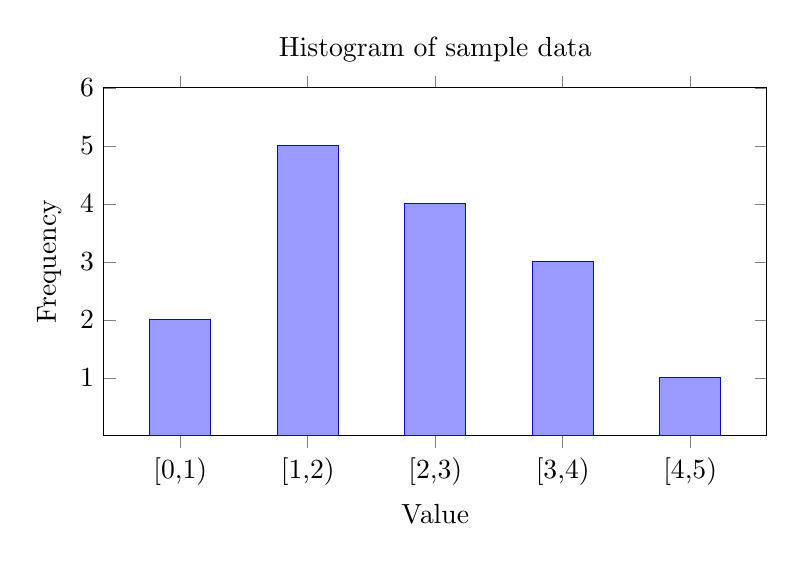
\begin{tikzpicture}
		\pgfplotsset{compat=1.18}
		\begin{axis}[
		    ybar,
		    ymin=0,
		    ymax=6,
		    bar width=22pt,
		    width=10cm,
		    height=6cm,
		    xlabel={Value},
		    ylabel={Frequency},
		    ytick={1,2,3,4,5,6},
		    xtick={1,2,3,4,5},
		    xticklabels={{[0,1)}, {[1,2)}, {[2,3)}, {[3,4)}, {[4,5)}},
		    enlarge x limits=0.15,
		    title={Histogram of \gls{sample} \gls{data}}
			]
		\addplot+[fill=blue!40] coordinates {(1,2) (2,5) (3,4) (4,3) (5,1)};
		\end{axis}
		\end{tikzpicture}
		\caption{A histogram consists of the fractions of \glspl{datapoint} that 
			fall within different value ranges (i.e., bins). Each bar height shows 
			the count of \glspl{sample} in the corresponding interval.}
			\label{fig:histogram_dict}
		\end{figure}
		See also: \gls{dataset}, \gls{datapoint}, \gls{sample}.},
	first={histogram},
	text={histogram}  
}

\newglossaryentry{bootstrap}
{name={bootstrap},
	description={For\index{bootstrap} the analysis of \gls{ml} methods, it is often 
	    	useful to interpret a given \gls{dataset} $\dataset = \big\{ \datapoint^{(1)}, \,\ldots, \,\datapoint^{(\samplesize)}\big\}$ 
		as a collection of (\glspl{realization} of) \gls{iid} \glspl{rv} with 
		common \gls{probdist} $\probdist$. In practice, the \gls{probdist} $\probdist$ 
		is unknown and must be estimated from $\dataset$. The idea of the bootstrap 
		method is to use the \gls{empiricaldistribution} $\probdist^{(\dataset)}$ 
		of $\dataset$ as an \gls{estimator} for $\probdist$ \cite{hastie01statisticallearning}:
		$$ \frac{1}{\samplesize} \big| \sampleidx: \datapoint^{(\sampleidx)} \in \mathcal{A} \big| \approx \prob{\mathcal{A}}.$$
		Repeatedly sampling from the \gls{empiricaldistribution}, which is equivalent 
		to sampling with replacement from $\dataset$ \cite{BoostrapBook}, 
		results in new \glspl{dataset} $\dataset^{(1)}, \,\ldots, \,\dataset^{(\nrbootstraps)}$, each containing 
		$\samplesize$ \glspl{datapoint}. We then use each of 
		those \glspl{dataset} for \gls{model} \gls{training} (e.g., via \gls{erm}), 
		resulting in the learned \glspl{hypothesis}
		$\widehat{\hypothesis}^{(1)}, \,\ldots, \,\learnthypothesis^{(\nrbootstraps)}.$ 
        		We can use these learned \glspl{hypothesis} to estimate important characteristics 
		of an \gls{ml} method such as \gls{bias}, \gls{variance}, or \gls{gengap} \cite{hastie01statisticallearning}.
		\\
		See also: \gls{iid}, \gls{rv}, \gls{probdist}, \gls{histogram}.},
	first={bootstrap},
	text={bootstrap}  
}

\newglossaryentry{featurespace}
{name={feature space},
	description={The\index{feature space} \gls{feature} space of a given \gls{ml} application 
		or method is constituted by all potential values that the \gls{featurevec} of a \gls{datapoint} can take on. 
		For \glspl{datapoint} described by a fixed number $\nrfeatures$ of numerical \glspl{feature}, 
		a common choice for the \gls{feature} space is the \gls{euclidspace} $\mathbb{R}^{\nrfeatures}$. 
		However, the mere presence of $\nrfeatures$ numeric \glspl{feature} does not imply that $\mathbb{R}^{\nrfeatures}$ 
		is the most appropriate representation of the \gls{feature} space. Indeed, the numerical \glspl{feature}  
		might be assigned to \glspl{datapoint} in a largely arbitrary or random manner, resulting 
		in \glspl{datapoint} that are randomly scattered throughout $\mathbb{R}^{\nrfeatures}$ 
		without any meaningful geometric structure. \Gls{featlearn} methods try to learn a 
		transformation of the original (potentially nonnumeric) \glspl{feature} to ensure a 
		more meaningful arrangement of \glspl{datapoint} in $\mathbb{R}^{\nrfeatures}$. 
		Three examples of \gls{feature} spaces are shown in Fig. \ref{fig_featurespace_dict}.
		\begin{figure}[H]
			\centering
			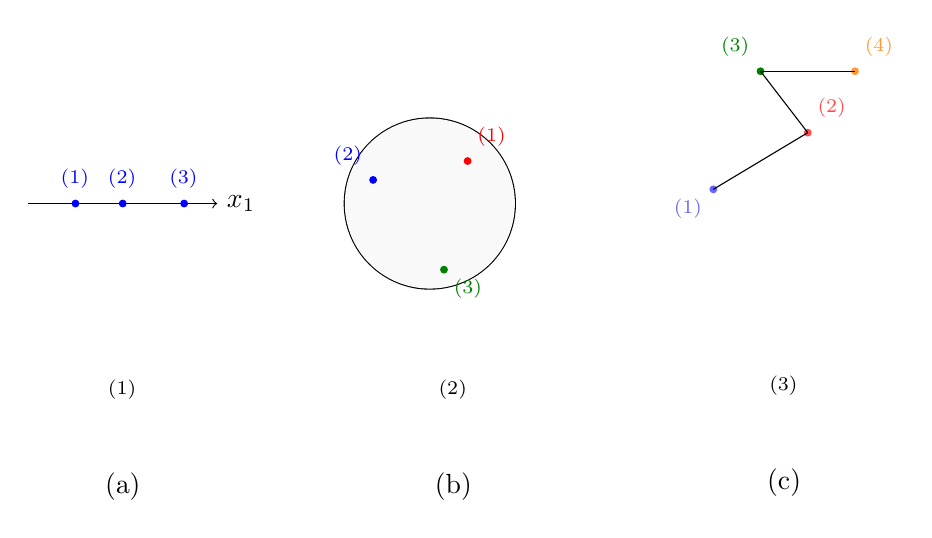
\begin{tikzpicture}[scale=0.6]
			% --------- 1D Line Feature Space (left) ---------
			\begin{scope}[xshift=0cm]
  				% Axis
 	 			\draw[->] (-0.5, 0) -- (3.5, 0) node[right] {$x_1$};
  				% Points
  				\foreach \x/\lbl in {0.5/$\featurevec^{(1)}$, 1.5/$\featurevec^{(2)}$, 2.8/$\featurevec^{(3)}$}
    				\filldraw[blue] (\x,0) circle (2pt) node[above] {\lbl};
  				% Label
  				\node at (1.5, -4.0)  {$\featurespace^{(1)}$};
				\node at (1.5, -6) {(a)};
			\end{scope}
			% --------- 2-D Bounded (Disk) Feature Space (middle) ---------
			\begin{scope}[xshift=8cm]
  				% Circle boundary
  				\draw[thick] (0,0) circle (1.8);
  				\fill[gray!5] (0,0) circle (1.8);
  				% Points inside circle
  				\filldraw[red] (0.8, 0.9) circle (2pt) node[anchor=south west] {$\featurevec^{(1)}$};
  				\filldraw[blue] (-1.2, 0.5) circle (2pt) node[anchor=south east] {$\featurevec^{(2)}$};
  				\filldraw[green!50!black] (0.3, -1.4) circle (2pt) node[anchor=north west] {$\featurevec^{(3)}$};
  				% Label
  				\node at (0.5, -4) {$\featurespace^{(2)}$};
				\node at (0.5, -6) {(b)};
			\end{scope}
			% --------- Graph-Based Feature Space (right) ---------
			\begin{scope}[xshift=14cm, yshift=0.3cm]
  				% Nodes
 	 			\filldraw[blue!60] (0,0) circle (2pt) node[anchor=north east] {$\featurevec^{(1)}$};
 	 			\filldraw[red!70] (2,1.2) circle (2pt) node[anchor=south west] {$\featurevec^{(2)}$};
  				\filldraw[green!50!black] (1,2.5) circle (2pt) node[anchor=south east] {$\featurevec^{(3)}$};
  				\filldraw[orange!80] (3,2.5) circle (2pt) node[anchor=south west] {$\featurevec^{(4)}$};
  				% Edges
  				\draw[-] (0,0) -- (2,1.2);
  				\draw[-] (2,1.2) -- (1,2.5);
  				\draw[-] (1,2.5) -- (3,2.5);
  				% Label
  				\node at (1.5, -4.2) {$\featurespace^{(3)}$};
				\node at (1.5, -6.2) {(c)};
			\end{scope}
			\end{tikzpicture}
		\caption{Three different \gls{feature} spaces. (a) A linear space $\featurespace^{(1)} = \mathbb{R}$. (b) A 
			bounded \gls{convex} set $\featurespace^{(2)} \subseteq \mathbb{R}^{2}$. (c) A discrete space 
			$\featurespace^{(3)}$ whose elements are nodes of an \gls{undirectedgraph}. \label{fig_featurespace_dict}}
		\end{figure}
		See also: \gls{featurevec}, \gls{euclidspace}.},
	first={feature space},
	text={feature space}  
}

\newglossaryentry{missingdata}
{name={missing data},
	description={Consider\index{missing data} a \gls{dataset} constituted by \glspl{datapoint} collected via 
		some physical \gls{device}. Due to imperfections and failures, some of the \gls{feature} 
		or \gls{label} values of \glspl{datapoint} might be corrupted or simply missing. 
		\Gls{data} imputation aims to estimate these missing values \cite{Abayomi2008DiagnosticsFM}. 
		We can interpret \gls{data} imputation as an \gls{ml} problem where the \gls{label} of a \gls{datapoint} is 
		the value of the corrupted \gls{feature}.
				\\
		See also: \gls{feature}, \gls{label}. },
	first={missing data},
	text={missing data}  
}

\newglossaryentry{hyperparameter}
{name={hyperparameter},
	description={A hyperparameter\index{hyperparameter} associated with an \gls{ml} method is 
		a quantity that is used to select among a family of \glspl{model}. 
		Typical examples include the \gls{learnrate} used in a \gls{gdmethod}, 
		the number of \glspl{feature} used in a \gls{linmodel}, or the 
		\gls{maximum} depth of a \gls{decisiontree}. The usefulness of a specific 
		hyperparameter choice can be assessed via \gls{validation}. Similar 
		to learning (or tuning) \glspl{modelparam} by \gls{erm} on a \gls{trainset}, 
		we can learn (or tune) hyperparameters via minimizing the \gls{valerr}. Thus, 
		in a sense, hyperparameters are higher-level \glspl{modelparam} that are learned 
		via a higher-level form of \gls{erm}, i.e., minimizing the \gls{valerr} obtained by 
		the trained \gls{model} with a given hyperparameter value. 
			\\ 
		See also: \gls{model}, \gls{validation}, \gls{modelparam}.},
	first={hyperparameter},
	text={hyperparameter},
	plural={hyperparameters},
	firstplural={hyperparameters}
}

\newglossaryentry{dataimputation}
{name={data imputation},
	description={See\index{data imputation} \gls{missingdata}.},
	first={data imputation},
	text={data imputation}  
}

\newglossaryentry{feature}
{name={feature},
	description={A\index{feature} feature of a \gls{datapoint} is one of its properties 
	    	that can be measured or computed easily without the need for human supervision. 
		For example, if a \gls{datapoint} is a digital image (e.g., stored as a \texttt{.jpeg} file), 
		then we could use the red–green–blue (RGB) intensities of its pixels as features. 
		Another example is shown in Fig.\ \ref{fig:audio_features_dict}, where the signal 
		\glspl{sample} of a finite-duration audio signal are used as its features.
		\begin{figure}[H]
		\centering
		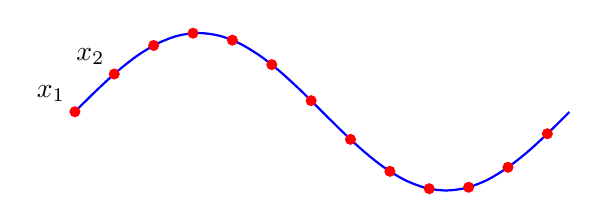
\begin{tikzpicture}[scale=1]
		% Draw a smooth waveform (sine curve as proxy for audio)
		\draw[thick, blue, domain=0:6.28, smooth, variable=\x] 
			plot ({\x}, {sin(\x r)});
		% Mark sample points at regular intervals
		\foreach \x [count=\i] in {0,0.5,...,6.28} {
			\fill[red] (\x, {sin(\x r)}) circle (2pt);
			% Label only the first two samples
			\ifnum\i=1
				\node[above left] at (\x, {sin(\x r)}) {$x_1$};
			\fi
			\ifnum\i=2
				\node[above left] at (\x, {sin(\x r)}) {$x_2$};
			\fi
		}
		\end{tikzpicture}
		\caption{An audio signal (blue waveform) and its discretized signal \glspl{sample} (red dots) that 
			can be used as its features $x_{1},\,\ldots,\,x_{\nrfeatures}$. \label{fig:audio_features_dict}}
		\end{figure}
		Domain-specific synonyms for the term feature are "\gls{covariate}," "explanatory variable," 
		"independent variable," "input (variable)," "\gls{predictor} (variable)," or "regressor" 
		\cite{Everitt2010}, \cite{Gujarati2021}, \cite{Dodge2003}. 
		\\
		See also: \gls{datapoint}.}, 
	first={feature},
	plural={features},
	text={feature}  
}

\newglossaryentry{featurevec}
{name={feature vector},
	description={\Gls{feature} \gls{vector} refers to a\index{feature vector} \gls{vector} $\vx = \big(x_{1}, \,\ldots, \,x_{\nrfeatures}\big)\,^{T}$ 
		whose entries are individual \glspl{feature} $x_{1}, \,\ldots, \,x_{\nrfeatures}$. Many \gls{ml} methods 
		use \gls{feature} \glspl{vector} that belong to some finite-dimensional \gls{euclidspace} $\mathbb{R}^{\nrfeatures}$. 
		For some \gls{ml} methods, however, it can be more convenient to work with \gls{feature} 
		\glspl{vector} that belong to an infinite-dimensional \gls{vectorspace} (e.g., see \gls{kernelmethod}). 
			\\
		See also: \gls{feature}, \gls{vector}, \gls{ml}, \gls{euclidspace}, \gls{vectorspace}.}, 
	first={feature vector},
	plural={feature vectors},
	firstplural={feature vectors},
	text={feature vector}  
}

\newglossaryentry{label}
{name={label},
	description={A label\index{label} is a higher-level fact or quantity of interest associated 
		with a \gls{datapoint}. For example, if the \gls{datapoint} is an image, the label 
		could indicate whether the image contains a cat 
		\cite{Everitt2010}, \cite{Gujarati2021}, \cite{Dodge2003}.
				\\
		See also: \gls{datapoint}, \gls{labelspace}.},
	first={label},
	plural={labels},
	text={label}  
}

\newglossaryentry{data}
{name={data},
	description={In the context of \gls{ml}, the term 
 		data\index{data} is often used as a synonym for \gls{dataset}
  		\cite{Everitt2010}, \cite{OxfordStatisticsDictionary}. 
  		The ISO/IEC 2382:2015 standard \cite{ISO2382} defines data as a \begin{quote} reinterpretable representation of 
  		information in a formalized manner suitable for communication, interpretation, or processing.\end{quote}
  		See also: \gls{dataset}, \gls{datapoint}, \gls{sample}.}, 
  	first={data},
	text={data}
}

\newglossaryentry{relational model}
{name={relational model},
	description={A relational \gls{model}\index{relational model} is a mathematical representation of \gls{data}. 
		The core idea is to ogranize \gls{data} as a collection of 
		tables (or relations) \cite{silberschatz2019database}, \cite{codd1970relational}. 
		A table consists of rows and columns, where each 
		row corresponds to a single \gls{datapoint}, and each 
		column represents a specific attribute of a \gls{datapoint}. 
		\gls{ml} methods use these attributes as the \glspl{feature} 
		and \gls{label} of a \gls{datapoint}. Table~\ref{tab:relmodel_dict} shows 
		a relational representation of a \gls{dataset} that consists of cows. 
		In the relational \gls{model}, the order of rows is immaterial, and each 
		attribute (i.e., column) is associated with a \gls{domain} that specifies the set 
		of admissible values. 
		In \gls{ml} applications, these attribute \glspl{domain} correspond to the 
		\gls{featurespace} and the \gls{labelspace}.
				\begin{table}[H]
					\refstepcounter{table}
					\caption*{
						\centering 
						\scshape TABLE \thetable \\[0.5ex]
						\scshape A Relation (or Table) That Represents the \gls{dataset} in Fig. \ref{fig_cows_dataset_dict} 
					}
					\label{tab:relmodel_dict} 
					\centering
					\begin{tabular}{lcccc}
						\hline
						\textbf{Name} & \textbf{Weight} & \textbf{Age} & \textbf{Height} & \textbf{Stomach temperature} \\
						\hline
						Zenzi & 100 & 4 & 100 & 25 \\
						Berta & 140 & 3 & 130 & 23 \\
						Resi  & 120 & 4 & 120 & 31 \\
						\hline
					\end{tabular}
				\end{table}
		See also: \gls{data}, \gls{datapoint}, \glspl{feature}, \gls{label}, \gls{dataset}.}, 
	first={relational model},
	text={relational model}
}
  		
\newglossaryentry{tabulardata}
{name={tabular data},
	description={Tabular \gls{data}\index{tabular data} consist of \glspl{datapoint} 
		that are characterized by a common set of attributes. These attributes 
		can be used as the \glspl{feature} or \glspl{label} of \glspl{datapoint}. 
		If the attributes are numeric, we can represent a \gls{dataset} by 
		a \gls{datamatrix} $\mathbf{D} \in \mathbb{R}^{\samplesize \times \nrfeatures}$, 
		where each of the $\samplesize$ rows corresponds to a single \gls{datapoint},
		and each of the $\nrfeatures$ columns represents a specific attribute \cite{Everitt2022}.
		\\
		See also: \gls{data}, \gls{datapoint}. }, 
	first={tabular data},
	text={tabular data}
}

\newglossaryentry{datamatrix}
{name={data matrix},
	description={See \gls{tabulardata}\index{data matrix}.}, 
	first={data matrix},
	firstplural={data matrices},
	plural={data matrices},
	text={data matrix}
}
		
\newglossaryentry{dataset}
{name={dataset},
	description={A\index{dataset} dataset is a set of distinct \glspl{datapoint}. 
		Strictly speaking, a dataset is an unordered collection of \glspl{datapoint} 
		that does not contain any repetitions. However, in \gls{ml} literature, the 
		term dataset is often used as a synonym for \gls{sample}, i.e., 
		a \gls{sequence} (or finite list) of \glspl{datapoint} that may contain repetitions. 
		\gls{ml} methods use datasets for \gls{model} \gls{training} and \gls{validation}. 
		The notion of a dataset is broad, i.e., \glspl{datapoint} may represent concrete 
		physical entities (such as humans or animals) or abstract objects (such as numbers). 
		For illustration, Fig.~\ref{fig_cows_dataset_dict} depicts a dataset whose 
		\glspl{datapoint} are cows.	
		\begin{figure}[H]
			\begin{center}
			\label{fig:cowsintheswissalps_dict}
			\includegraphics[width=0.5\textwidth]{assets/CowsAustria.jpg}
		  	\end{center}
			\caption{\label{fig_cows_dataset_dict}A cow herd somewhere in the Alps.}
	 	\end{figure}
		Quite often, an \gls{ml} engineer does not have direct access to the underlying dataset. 
		For instance, accessing the dataset in Fig.~\ref{fig_cows_dataset_dict} would require 
		visiting the cow herd. In practice, we work with a more convenient 
		representation (or approximation) of the dataset. Various mathematical \glspl{model} 
		have been developed for this purpose \cite{silberschatz2019database}, \cite{abiteboul1995foundations}, 
		\cite{hoberman2009data}, \cite{ramakrishnan2002database}. One of the most widely used is 
		the \gls{relational model}, which organizes \gls{data} as a table (or relation) 
		\cite{silberschatz2019database}, \cite{codd1970relational}. A table consists of 
		rows and columns, where each row corresponds to a single \gls{datapoint}, and each 
		column represents a specific attribute of a \gls{datapoint}. 
		\gls{ml} methods typically interpret these attributes as \glspl{feature} 
		or as a \gls{label} of a \gls{datapoint}. As an illustration, 
		Table~\ref{tab:cowdata_dict} shows a relational representation of the 
		dataset from Fig.~\ref{fig_cows_dataset_dict}. In the \gls{relational model}, 
		the order of rows is immaterial, and each attribute (i.e., column) is associated with a 
		\gls{domain} that specifies the set of admissible values. In \gls{ml} applications, 
		these attribute \glspl{domain} correspond to the \gls{featurespace} and the \gls{labelspace}.
		\begin{table}[H]
			\refstepcounter{table}
			\caption*{
				\centering 
				\scshape TABLE \thetable \\[0.5ex]
				\scshape A Relation (or Table) That Represents the Dataset in Fig. \ref{fig_cows_dataset_dict} 
			}
			\label{tab:cowdata_dict} 
			\centering
			\begin{tabular}{lcccc}
				\hline
				\textbf{Name} & \textbf{Weight} & \textbf{Age} & \textbf{Height} & \textbf{Stomach temperature} \\
				\hline
				Zenzi & 100 & 4 & 100 & 25 \\
				Berta & 140 & 3 & 130 & 23 \\
				Resi  & 120 & 4 & 120 & 31 \\
				\hline
			\end{tabular}
		\end{table}
 		While the \gls{relational model} is useful for the study of many \gls{ml} applications, 
		it may be insufficient regarding the requirements for \gls{trustAI}. Modern 
 		approaches like datasheets for datasets provide more comprehensive 
 		documentation, including details about the \gls{data} collection process, intended 
 		use, and other contextual information \cite{DatasheetData2021}.
 		\\
		See also: \gls{datapoint}, \gls{sample}, \gls{data}, \gls{feature}, \gls{featurespace}, \gls{labelspace}.},
	first={dataset},
	plural={datasets},
	text={dataset}  
}

\newglossaryentry{predictor}
{name={predictor},
	description={A\index{predictor} predictor is a real-valued \gls{hypothesis} \gls{map}. 
		Given a \gls{datapoint} with \glspl{feature} $\featurevec$, the value 
		$\hypothesis(\featurevec) \in \mathbb{R}$ is used as a \gls{prediction} for the true 
		numeric \gls{label} $\truelabel \in \mathbb{R}$ of the \gls{datapoint}.
				\\
		See also: \gls{hypothesis}, \gls{map}, \gls{datapoint}, \gls{feature}, \gls{prediction}, \gls{label}. },
	first={predictor},
	text={predictor}  
}

\newglossaryentry{labeled datapoint}
{name={labeled data point},
 	description={A\index{labeled data point} \gls{datapoint} whose \gls{label} is known or has been determined 
 		by some means that might require human labor.
			\\
		See also: \gls{datapoint}, \gls{label}.},
 	first={labeled data point},
	plural={labeled data points},
	firstplural={labeled data points},
 	text={labeled data point}  
}
 
\newglossaryentry{samplespace}
{name={sample space}, 
  	description={A\index{sample space} \gls{sample} space is the set of all possible 
		\glspl{outcome} of a \gls{randomexperiment} \cite{BillingsleyProbMeasure}, 
		\cite{BertsekasProb}, \cite{AshProbMeasure}, \cite{papoulis}. 
		\\
 		See also: \gls{probspace}.},  
  	first={sample space}, 
 	firstplural={sample spaces},
 	plural={sample spaces},
  	text={sample space}
} 
	
\newglossaryentry{realization}
{name={realization},
	description={Consider\index{realization} an \gls{rv} $\featurevec$ that maps each \gls{outcome} 
		$\outcome \in \samplespace$ of a \gls{probspace} to an element $a$ of a 
		\gls{measurable} space $\mathcal{N}$ \cite{RudinBookPrinciplesMatheAnalysis}, \cite{BillingsleyProbMeasure}, \cite{HalmosMeasure}. 
		A realization of $\featurevec$ is any element $\va \in \mathcal{N}$ such that there exists 
		an element $\outcome' \in \samplespace$ with $\featurevec(\outcome') = \va$.
			\\
		See also: \gls{rv}, \gls{outcome}, \gls{probspace}, \gls{measurable}.}, 
	first={realization},
	plural={realizations},
	text={realization}  
}

\newglossaryentry{trainset}
{name={training set},
	description={A\index{training set} \gls{training} set is a \gls{dataset} $\dataset$ that consists of some \glspl{datapoint} used in \gls{erm} 
		to learn a \gls{hypothesis} $\learnthypothesis$. The average \gls{loss} of $\learnthypothesis$ on the 
		\gls{training} set is referred to as the \gls{trainerr}. The comparison of the \gls{trainerr} with the 
		\gls{valerr} of $\learnthypothesis$ allows us to diagnose the \gls{ml} method and informs how to improve 
		the \gls{valerr} (e.g., using a different \gls{hypospace} or collecting more \glspl{datapoint}) \cite[Sec. 6.6]{MLBasics}.
			\\
		See also: \gls{training}, \gls{dataset}, \gls{datapoint}, \gls{erm}, \gls{hypothesis}, \gls{loss}, \gls{trainerr}, \gls{valerr}, \gls{ml}, \gls{hypospace}.},
	first={training set},
	plural={training sets},
	firstplural={training sets},
	text={training set}  
}

\newglossaryentry{netmodel}
{name={networked model},
 	description={A\index{networked model} networked \gls{model} over an \gls{flnetwork} $\graph = \pair{\nodes}{\edges}$ assigns 
   		a \gls{localmodel} (i.e., a \gls{hypospace}) to each node $\nodeidx \in \nodes$ of the \gls{flnetwork} $\graph$.
   		\\
		See also: \gls{model}, \gls{flnetwork}, \gls{localmodel}, \gls{hypospace}.}, 
   first={networked model},
   text={networked model}  
}

\newglossaryentry{batch}
{name={batch},
	description={In\index{batch} the context of \gls{stochGD}, a batch refers to a randomly 
		chosen subset of the overall \gls{trainset}. We use the \glspl{datapoint} in this subset 
		to estimate the \gls{gradient} of \gls{trainerr} and, in turn, to update the \glspl{modelparam}.
			\\
		See also: \gls{stochGD}, \gls{trainset}, \gls{datapoint}, \gls{gradient}, \gls{trainerr}, \gls{modelparam}.}, 
 	first={batch},
 	firstplural={batches}, 
 	plural={batches}, 
 	text={batch}  
}

\newglossaryentry{epoch}
{name={epoch},
	description={An epoch\index{epoch} represents one complete pass of the entire \gls{trainset} through some learning 
		\gls{algorithm}. It refers to the point at which a \gls{model} has processed every \gls{datapoint} in the \gls{trainset} once. 
		\Gls{training} a \gls{model} usually requires multiple epochs, since each \gls{iteration} allows the \gls{model} to refine the 
		\glspl{parameter} and improve \glspl{prediction}. The number of epochs is something predefined by the user,  
		and thus a \gls{hyperparameter}, which plays a crucial role in determining how the \gls{model} will generalize to unseen \gls{data}. 
		Too few epochs will result in \gls{underfitting}, while too many epochs can result in \gls{overfitting}.
		\\
		See also: \gls{trainset}, \gls{algorithm}, \gls{model}, \gls{datapoint}, \gls{parameter}, \gls{prediction}, \gls{underfitting}, \gls{overfitting}.},
	first={epoch},
	text={epoch}
} 

\newglossaryentry{netdata}
{name={networked data},
	description={Networked\index{networked data} \gls{data} consist of \glspl{localdataset} 
		that are related by some notion of pairwise similarity. We can represent networked 
		\gls{data} using a \gls{graph} whose nodes carry \glspl{localdataset} and whose edges encode 
		pairwise similarities. An example of networked \gls{data} can be found in \gls{fl} applications 
		where \glspl{localdataset} are generated by spatially distributed \glspl{device}.
			\\
		See also: \gls{data}, \gls{localdataset}, \gls{graph}, \gls{fl}, \gls{device}.}, 
	first={networked data},
	text={networked data}  
}

\newglossaryentry{trainerr}
{name={training error},
	description={\Gls{training} error is the\index{training error} average \gls{loss} of a \gls{hypothesis} when 
		predicting the \glspl{label} of the \glspl{datapoint} in a \gls{trainset}. 
		We sometimes also refer to \gls{training} error as the minimal average \gls{loss} 
		that is achieved by a solution of \gls{erm}.
				\\
		See also: \gls{loss}, \gls{hypothesis}, \gls{label}, \gls{datapoint}, \gls{trainset}, \gls{erm}.},
	first={training error},
	text={training error}  
}

\newglossaryentry{datapoint}
{name={data point},
	description={A\index{data point} \gls{data} point is any object that conveys information~\cite{coverthomas}. 
		Examples include students, radio signals, trees, images, \glspl{rv}, real numbers, 
 		or proteins. We describe \gls{data} points of the same type by two categories 
		of properties. The first category includes \glspl{feature} that are \gls{measurable} or 
		computable properties of a \gls{data} point. These attributes can be automatically extracted 
		or computed using sensors, computers, or other \gls{data} collection systems. For a \gls{data} 
		point that represents a patient, one \gls{feature} could be the body weight.
		The second category includes \glspl{label} that are higher level facts (or quantities of interest)—that is, 
		facts that typically require human expertise or domain knowledge to determine rather than being directly 
		\gls{measurable}—associated with the \gls{data} point. For a \gls{data} point that represents a patient, 
		a cancer diagnosis provided by a physician would serve as the \gls{label}. 
		Fig.\ \ref{fig:datapoint_cowherd_dict} depicts an image as an example of a \gls{data} 
		point along with its \glspl{feature} and \glspl{label}. Importantly, what constitutes 
		a \gls{feature} or a \gls{label} is not inherent to the \gls{data} point itself—it is a design 
		choice that depends on the specific \gls{ml} application.
		\begin{figure}[H]
    		\centering
    			% Image as a datapoint
    			\begin{minipage}[t]{0.95\textwidth}
        			\centering
        			\includegraphics[width=\textwidth]{assets/CowsAustria.jpg}
        			\caption*{A single \gls{data} point.}
        			\vspace{5mm}
    			\end{minipage}
    			% Feature and label description
    			\begin{minipage}[t]{0.95\textwidth}
        			\Glspl{feature}:
        			\begin{itemize}
            			\item $x_{1}, \,\ldots, \,x_{\nrfeatures}$: Color intensities of all image pixels.
            			\item $x_{\nrfeatures+1}$: Time-stamp of the image capture.
            			\item $x_{\nrfeatures+2}$: Spatial location of the image capture.
			\end{itemize}
			\Glspl{label}:
            		\begin{itemize}
               	 		\item $\truelabel_{1}$: Number of cows depicted. 
                			\item $\truelabel_{2}$: Number of wolves depicted. 
                			\item $\truelabel_{3}$: Condition of the pasture (e.g., healthy, overgrazed).
            		\end{itemize}
    			\end{minipage}
    		\caption{Illustration of a \gls{data} point consisting of an image. We can use 
			different properties of the image as \glspl{feature} and higher level facts
			about the image as \glspl{label}.\label{fig:datapoint_cowherd_dict}}
		\end{figure}
 		The distinction between \glspl{feature} and \glspl{label} is not always clear-cut. 
 		A property that is considered a \gls{label} in one setting (e.g., a cancer diagnosis) 
 		may be treated as a \gls{feature} in another setting—particularly if reliable automation (e.g., 
 		via image analysis) allows it to be computed without human intervention.
   		\Gls{ml} broadly aims to predict the \gls{label} of a \gls{data} point based on its \glspl{feature}. 
				\\
		See also: \gls{data}, \gls{feature}, \gls{label}, \gls{dataset}.}, 
	first={data point},
	plural={data points},
	firstplural={data points},
	text={data point}  
}

\newglossaryentry{valerr}
{name={validation error},
 	description={Consider\index{validation error} a \gls{hypothesis} $\learnthypothesis$ that is 
 		obtained by some \gls{ml} method, e.g., using \gls{erm} on a \gls{trainset}. The average \gls{loss} 
 		of $\learnthypothesis$ on a \gls{valset}, which is different from the \gls{trainset}, is referred 
 		to as the \gls{validation} error.
			\\
		See also: \gls{hypothesis}, \gls{ml}, \gls{erm}, \gls{trainset}, \gls{loss}, \gls{valset}, \gls{validation}.},
	first={validation error},
	plural={validation errors},
	firstplural={validation errors},
	text={validation error}  
}

\newglossaryentry{validation} 
{name={validation},
	description={Consider\index{validation} a \gls{hypothesis} $\learnthypothesis$ 
		that has been learned via some \gls{ml} method, e.g., by solving \gls{erm} 
	   	on a \gls{trainset} $\dataset$. 
		Validation refers to the process of evaluating the \gls{loss} incurred by the 
		\gls{hypothesis} $\learnthypothesis$ on a set of 
		\glspl{datapoint} that are not contained in the \gls{trainset} $\dataset$. This 
		set of \glspl{datapoint} is called the \gls{valset}. The average \gls{loss} of 
		$\learnthypothesis$ on the \gls{valset} is referred to as the \gls{valerr}. 
		An example of validation is shown in Fig. \ref{fig_validation_dict}.
		\begin{figure}[H] 
			\centering
			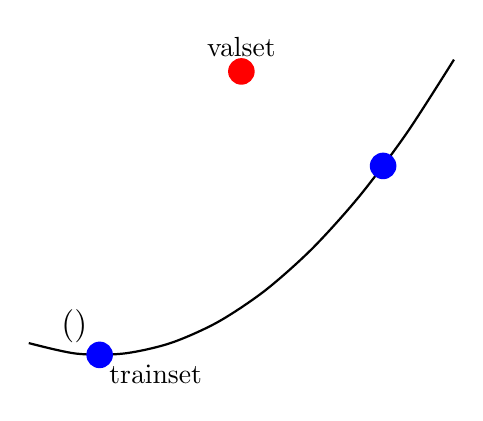
\begin{tikzpicture}[scale=1.2,x=1.5cm]
				% Straight line: y = x
				%	\draw[thick] (-0.5,-0.5) -- (2.5,2.5)
				%	node[pos=1, below right]
				%	{$\hypothesis'(\feature)=\feature$};
				% Quadratic: y = 0.5 x^2
				\draw[thick, domain=-0.5:2.5, samples=10, smooth]
				plot (\x,{0.5*\x*\x})
				node[pos=0, above left]
				{$\learnthypothesis(\feature)$};
				% Training data points
				\fill[blue] (0,0) circle (4pt);
				\fill[blue] (2,2) circle (4pt);
				% Manual legend
				\node[below right] at (0,0) {\gls{trainset}};
				% validation data point 
				\fill[red] (1,3) circle (4pt);
				\node[above,yshift=2pt] at (1,3) {\gls{valset}};
			\end{tikzpicture}
		\caption{Illustration of validation. The blue points represent the \glspl{datapoint} in the 
			\gls{trainset}, while the red point represents a \gls{datapoint} in the \gls{valset}. The 
			\gls{hypothesis} $\learnthypothesis$ (black curve) fits the \glspl{datapoint} in the \gls{trainset} perfectly, 
			but incurs a large \gls{loss} on the \gls{datapoint} in the \gls{valset}. \label{fig_validation_dict}}
		\end{figure} 
		See also: \gls{trainset}, \gls{valset}, \gls{valerr}, \gls{overfitting}, \gls{generalization}, \gls{kfoldcv}, \gls{loo}.},
 first={validation},
 text={validation}  
}

\newglossaryentry{quadfunc}
{name={quadratic function},
	description={A quadratic \gls{function}\index{quadratic function} is a \gls{function} $f: \mathbb{R}^{\nrfeatures} \rightarrow \mathbb{R}$ 
		of the following form: 
		$$f(\weights) =  \weights\,^{T} \mathbf{Q} \mathbf{w} + \mathbf{q}\,^{T} \weights+a$$ with 
		some \gls{matrix} $\mQ \in \mathbb{R}^{\nrfeatures \times \nrfeatures}$, \gls{vector} $\vq \in \mathbb{R}^{\nrfeatures}$, 
		and scalar $a \in \mathbb{R}$.
		\\
		See also: \gls{function}, \gls{matrix}, \gls{vector}. },
	first={quadratic function},
	text={quadratic function}  
}

\newglossaryentry{valset}
{name={validation set},
 	description={A\index{validation set} set of \glspl{datapoint} used to estimate 
  		the \gls{risk} of a \gls{hypothesis} $\learnthypothesis$ that has been learned by some 
  		\gls{ml} method (e.g., solving \gls{erm}). The average \gls{loss} of $\learnthypothesis$ 
  		on the \gls{validation} set is referred to as the \gls{valerr} and can be used to diagnose an 
  		\gls{ml} method (see \cite[Sec. 6.6]{MLBasics}). The comparison between \gls{trainerr} 
  		and \gls{valerr} can inform directions for the improvement of the \gls{ml} method (such as 
  		using a different \gls{hypospace}).
			\\
		See also: \gls{datapoint}, \gls{risk}, \gls{hypothesis}, \gls{ml}, \gls{erm}, \gls{loss}, \gls{validation}, 
		\gls{valerr}, \gls{trainerr}, \gls{hypospace}, \gls{kfoldcv}, \gls{loo}.},
	first={validation set},
	text={validation set},
	plural={validation sets}
}

\newglossaryentry{testset}
{name={test set},
	description={A\index{test set} set of \glspl{datapoint} that have  
		been used neither to train a \gls{model} (e.g., via \gls{erm}) nor 
		to choose between different \glspl{model} in a \gls{valset}.
				\\
		See also: \gls{datapoint}, \gls{model}, \gls{erm}, \gls{valset}.},
	first={test set},
	text={test set}  
}

\newglossaryentry{modelsel}
{name={model selection},
	description={In\index{model selection} \gls{ml}, \gls{model} selection refers to the 
		process of choosing between different candidate \glspl{model}. In its most 
		basic form, \gls{model} selection amounts to the following steps \cite[Ch. 6]{MLBasics}: 
		\begin{enumerate}[label=\arabic*)]
			\item \gls{training} each candidate \gls{model}; 
			\item computing the \gls{valerr} for each trained \gls{model}; 
			\item choosing the \gls{model} with the smallest \gls{valerr}. 
		\end{enumerate}
		See also: \gls{ml}, \gls{model}, \gls{training}, \gls{valerr}.},
	first={model selection},
	text={model selection}  
}

\newglossaryentry{linclass}
{name={linear classifier}, 
	description={Consider\index{linear classifier} \glspl{datapoint} characterized by numeric \glspl{feature} $\featurevec \in \mathbb{R}^{\nrfeatures}$ 
	    	and a \gls{label} $\truelabel \in \labelspace$ from some finite \gls{labelspace} $\labelspace$. 
		A linear \gls{classifier} is characterized by having \glspl{decisionregion} that are 
		separated by \glspl{hyperplane} in $\mathbb{R}^{\featuredim}$ \cite[Ch. 2]{MLBasics}.
				\\
		See also: \gls{datapoint}, \gls{feature}, \gls{label}, \gls{labelspace}, \gls{classifier}, \gls{decisionregion}.},
	first={linear classifier},
	text={linear classifier} 
}

\newglossaryentry{erm}
{name={empirical risk minimization (ERM)}, 
	description={ERM\index{empirical risk minimization (ERM)} is the \gls{optproblem} of 
		selecting a \gls{hypothesis} $\learnthypothesis \in \hypospace$ that minimizes the 
		average \gls{loss} (or \gls{emprisk}) on a \gls{trainset} $\dataset$. 
		The \gls{hypothesis} is chosen from a \gls{hypospace} (or \gls{model}) $\hypospace$. 
		The \gls{dataset} $\dataset$ is referred to as \gls{trainset}. A plethora of ERM-based 
		\gls{ml} methods is obtained for different design choices for the \gls{dataset}, \gls{model}, 
		and \gls{loss} \cite[Ch. 3]{MLBasics}. Fig.\ \ref{fig_erm_dict} illustrates ERM for a \gls{linmodel} 
		and \glspl{datapoint} that are characterized by a single \gls{feature} $\feature$ and a \gls{label} $\truelabel$. 
		The \gls{hypothesis} $\hypothesis$ is a \gls{linearmap} that predicts the \gls{label} 
		of a \gls{datapoint} as a linear \gls{function} of its \gls{feature} $\feature$, i.e., 
		$\hypothesis(\feature) = \weight_{1} \feature + \weight_{0}$, where $\weight_{1}$ 
		and $\weight_{0}$ are the \glspl{modelparam} of the \gls{hypothesis} $\hypothesis$. 
		The ERM problem is to find the \glspl{modelparam} $\weight_{1}$ and $\weight_{0}$ that 
		minimize the average \gls{loss} (or \gls{emprisk}) incurred by the \gls{hypothesis} 
		$\hypothesis$ on the \gls{trainset} $\dataset$.
    		\begin{figure}[H]
			\begin{center}
			\begin{tikzpicture}[scale=1]
  			\def\slope{0.4}
 	 		\def\intercept{2.0}
  			\def\xmin{0}
 		 	\def\xmax{6.5}
  			\draw[color=black, thick, dashed, domain=\xmin:\xmax, variable=\x] plot ({\x},{\slope*\x + \intercept}); 
			% Place label at the endpoint (xmax, h(xmax))
   			\coordinate (hend) at (\xmax,{\slope*\xmax + \intercept});
			\node[above right] at (hend) {$\hypothesis(\feature)$};
   			\foreach \i/\xval/\yval in {1/1.2/1.8, 2/3.0/2.6, 3/5.0/5.7} {
      			% predicted label on the hypothesis line
      			\coordinate (l\i) at (\xval, {\slope*\xval + \intercept});
      			% actual label
      			\coordinate (n\i) at (\xval, \yval);
      			% draw data point
      			\node[circle,draw,fill=blue,minimum size=6pt,scale=0.6] (pt\i) at (n\i) {};
      			% residual arrow
      			\draw[<->, color=blue, thick] (l\i) -- (n\i);
  			}
  			% Labels for data points
  			\node[anchor=west,below,yshift=-2pt] at (n1) {$\big(\feature^{(1)},\,\truelabel^{(1)}\big)$};
  			\node[anchor=west,below]        at (n2) {$\big(\feature^{(2)},\,\truelabel^{(2)}\big)$};
  			\node[anchor=west,above]   at (n3) {$\big(\feature^{(3)},\,\truelabel^{(3)}\big)$};
			\end{tikzpicture}
		\caption{ERM learns a \gls{hypothesis} $\hypothesis \in \hypospace$ 
			out of a \gls{model} $\hypospace$ by minimizing the average \gls{loss} (or \gls{emprisk}) 
			$1/\samplesize \sum_{\sampleidx=1}^\samplesize \lossfunc{\pair{\featurevec^{(\sampleidx)}}{ \truelabel^{(\sampleidx)}}}				{\hypothesis}$ 
			incurred on a \gls{trainset} $\dataset$.} \label{fig_erm_dict}
			\end{center}
		\end{figure}
		See also: \gls{optproblem}, \gls{loss}, \gls{emprisk}, \gls{trainset}, \gls{optmethod}.},
	first={empirical risk minimization (ERM)},
	text={ERM} 
}

\newglossaryentry{sampleweighting}
{name={sample weighting}, 
	description={Consider\index{sample weighting} an \gls{erm}-based method that 
		learns a \gls{hypothesis} by minimizing the average \gls{loss} on a \gls{trainset}. 
		In its basic form, \gls{erm} treats all \glspl{datapoint} equally important. 
		However, in some applications, it can be useful to put different emphasis on the 
		\gls{prediction} errors obtained for different \glspl{datapoint}. For example, 
		if a \gls{datapoint} is considered an \gls{outlier} we should reduce its influence 
		on the learned \gls{hypothesis}. 
		We can implement this idea by assigning a nonnegative weight 
		$\sampleweight{\sampleidx}$ to each \gls{datapoint} 
		$\pair{\featurevec^{(\sampleidx)}}{\truelabel^{(\sampleidx)}}$ in the \gls{trainset}. 
    		This results in the following weighted \gls{erm} principle:
		\begin{equation}
			\label{equ_weighted_erm_dict}
			\min_{\hypothesis \in \hypospace} \sum_{\sampleidx=1}^{\samplesize} 
			  \sampleweight{\sampleidx} \, \lossfunc{\pair{\featurevec^{(\sampleidx)}}{\truelabel^{(\sampleidx)}}}{\hypothesis}. 
		\end{equation}
		Fig.~\ref{fig_sampleweighting_dict} illustrates the concept of a 
		\gls{trainset} of three \glspl{datapoint} that contribute unequally to the \gls{emprisk}.
    		\begin{figure}[H]
    			\begin{center}
        			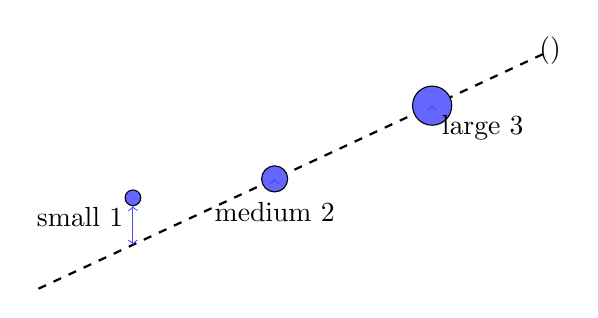
\begin{tikzpicture}[yscale=0.3]
      			% hypothesis line fitted (almost) to medium & large points
      			\def\slope{1.55}
      			\def\intercept{-2.05}
      			\draw[thick,dashed,domain=0:6.5,variable=\x]
        			plot({\x},{\slope*\x+\intercept});
      			\node[] at (6.5,{\slope*6.5+\intercept}) {$\hypothesis(\feature)$};
      			% three data points with varying weights (sizes)
      			\foreach \i/\xval/\yval/\scaleval in {1/1.2/1.8/0.6, 2/3.0/2.6/1.0, 3/5.0/5.7/1.5} {
        			\node[circle,draw,fill=blue!60,minimum size=6pt,scale=\scaleval]
          		(pt\i) at (\xval,\yval) {};
        			\draw[<->,color=blue!70] (\xval,{\slope*\xval+\intercept}) -- (pt\i);
      			}
      			\node[below left] at (pt1) {small $\sampleweight{1}$};
      			\node[below, yshift=-5pt]  at (pt2) {medium $\sampleweight{2}$ };
      			\node[below right]at (pt3) {large $\sampleweight{3}$};
    			\end{tikzpicture}
      		\caption{\Gls{sample} weighting assigns each \gls{datapoint} of a \gls{trainset} 
	  		a weight $\sampleweight{\sampleidx}$. Assigning a small weight 
	  		(such as $\sampleweight{1}$ in this example) to a 
	  		\gls{datapoint} decreases its influence on the \gls{hypothesis} 
	 		learned via solving \eqref{equ_weighted_erm_dict}.}
      			\label{fig_sampleweighting_dict}
    			\end{center}
    		\end{figure}
		See also: \gls{erm}, \gls{outlier}, \gls{adaboost}.},
	first={sample weighting}, 
	text={sample weighting}
}

\newglossaryentry{multilabelclass}
{name={multi-label classification}, 
	description={Multi-\gls{label} 
		\gls{classification}\index{multi-label classification} problems and methods use \glspl{datapoint} 
		that are characterized by several \glspl{label}. As an example, consider a \gls{datapoint} 
		representing a picture with two \glspl{label}. One \gls{label} indicates the presence of a human 
		in this picture and another \gls{label} indicates the presence of a car.
				\\
		See also: \gls{label}, \gls{classification}, \gls{datapoint}.},
	    first={multi-label classification},
	    text={multi-label classification} 
}

\newglossaryentry{inference}
{name={inference}, 
	description={In the context of \gls{ml}, inference\index{inference} refers to the process 
		of evaluating a learned \gls{hypothesis} (or trained \gls{model}) $\learnthypothesis(\featurevec)$ 
		based on the \glspl{feature} of a \gls{datapoint} \cite{BishopBook}, \cite{Murphy2012}. 
		A basic \gls{ml} workflow starts with \gls{model} \gls{training} and then 
		uses the trained \gls{model} for inference. 
				\\
		See also: \gls{model}, \gls{loss}, \gls{erm}.},
	first={inference},
	text={inference}
}

\newglossaryentry{training}
{name={training}, 
	description={In the context of \gls{ml}, training\index{training} refers to the process 
		of learning a useful \gls{hypothesis} $\learnthypothesis$ out of a \gls{model} $\hypospace$. 
		The training of a \gls{model} $\hypospace$ is guided by the \gls{loss} incurred on a set 
		of \glspl{datapoint}, which serve as the \gls{trainset}. For \glspl{parammodel}, 
		where each \gls{hypothesis} $\hypothesis^{(\weights)}$ is characterized by a specific 
		choice for the \glspl{modelparam}, training amounts to finding an optimal choice for the 
		\glspl{modelparam} $\weights$. A widely-used approach to training is \gls{erm}, which 
		learns a \gls{hypothesis} by minimizing the average \gls{loss} incurred on a \gls{trainset}. 
		One of the main challenges in \gls{ml} is to control the \gls{discrepancy} between the 
		\gls{loss} incurred on the \gls{trainset} and the \gls{loss} incurred on other (unseen) \glspl{datapoint}.
				\\
		See also: \gls{model}, \gls{loss}, \gls{erm}.},
	first={training},
	text={training}, 
	user1={trained}
}

\newglossaryentry{ssl}
{name={semi-supervised learning (SSL)}, 
	description={SSL\index{semi-supervised learning (SSL)} methods use unlabeled \glspl{datapoint}
		to support the learning of a \gls{hypothesis} from \glspl{labeled datapoint} \cite{SemiSupervisedBook}. 
		This approach is particularly useful for \gls{ml} applications that offer a large number of 
		unlabeled \glspl{datapoint}, but only a limited number of \glspl{labeled datapoint}.
			\\
		See also: \gls{datapoint}, \gls{hypothesis}, \gls{labeled datapoint}, \gls{ml}.}, 
	first={semi-supervised learning (SSL)},
	text={SSL} 
}
	
\newglossaryentry{objfunc}
{name={objective function},
	description={An\index{objective function} objective \gls{function} is a \gls{map} that assigns a numeric 
		objective value $f(\weights)$ to each choice $\weights$ of some variable that we want to 
		optimize (see Fig. \ref{fig_obj_func_dict}). In the context of \gls{ml}, the \gls{optimization} variable could 
		be the \glspl{modelparam} of a \gls{hypothesis} $\hypothesis^{(\weights)}$. 
		Common objective \glspl{function} include the \gls{risk} (i.e., expected \gls{loss}) or the \gls{emprisk} 
		(i.e., average \gls{loss} over a \gls{trainset}). \gls{ml} methods apply \gls{optimization} 
		techniques, such as \glspl{gdmethod}, to find the choice $\weights$ with the 
		optimal value (e.g., the \gls{minimum} or the \gls{maximum}) of the objective \gls{function}.
		\begin{figure}[H]
			\begin{center}
			\begin{tikzpicture}[scale=1.0]
				% Axes
				\draw[->] (-0.5,0) -- (4.5,0) node[right] {$\weights$};
				\draw[->] (0,-0.5) -- (0,3.5);
				% Objective function curve
				\draw[thick,domain=0.3:4,smooth,variable=\x] 
				plot ({\x}, {0.5*(\x-2)^2 + 0.5});
				% Label the curve
				\node at (3.5,2.8) {$f(\weights)$};
			\end{tikzpicture} 
			\end{center}
		\caption{An objective \gls{function} maps each possible value $\weights$ of an 
		\gls{optimization} variable, such as the \glspl{modelparam} of an \gls{ml} \gls{model}, 
		to a value $f(\weights)$ that measures the usefulness of $\weights$.\label{fig_obj_func_dict}}
		\end{figure} 
		See also: \gls{loss}, \gls{emprisk}, \gls{erm}, \gls{optproblem}.},
	first={objective function},
	plural={objective functions}, 
	firstplural={objective functions}, 
	text={objective function} 
}
	
\newglossaryentry{regularizer}
{name={regularizer}, 
	description={A regularizer\index{regularizer} 
		assigns each \gls{hypothesis} $\hypothesis$ from a \gls{hypospace} $\hypospace$ a quantitative 
		\gls{measure} $\regularizer{\hypothesis}$ conveying to what extent its \gls{prediction} errors might differ 
		on \glspl{datapoint} on and outside a \gls{trainset}. \Gls{ridgeregression} 
		uses the regularizer $\regularizer{\hypothesis} \defeq \normgeneric{\weights}{2}^{2}$ for linear \gls{hypothesis} 
		\glspl{map} $\hypothesis^{(\weights)}(\featurevec) \defeq \weights\,^{T} \featurevec$ \cite[Ch. 3]{MLBasics}. 
		\Gls{lasso} uses the regularizer $\regularizer{\hypothesis} \defeq \normgeneric{\weights}{1}$ 
		for linear \gls{hypothesis} \glspl{map} $\hypothesis^{(\weights)}(\featurevec) \defeq \weights\,^{T} \featurevec$ \cite[Ch. 3]{MLBasics}.
				\\
		See also: \gls{ridgeregression}, \gls{lasso}, \gls{loss}, \gls{objfunc}. },
	first={regularizer},
	text={regularizer} 
}

\newglossaryentry{regularization}
{name={regularization}, 
	description={A\index{regularization} key challenge of modern \gls{ml} applications is that they often 
		use large \glspl{model}, which have an \gls{effdim} in the order of billions. 
		\Gls{training} a high-dimensional \gls{model} using basic \gls{erm}-based methods
		is prone to \gls{overfitting}, i.e., the learned \gls{hypothesis} performs well on the \gls{trainset} 
		but poorly outside the \gls{trainset}. Regularization refers to modifications of a given instance 
		of \gls{erm} in order to avoid \gls{overfitting}, i.e., to ensure that the learned \gls{hypothesis} does 
		not perform much worse outside the \gls{trainset}. There are three routes for implementing 
		regularization: 
		\begin{enumerate}[label=\arabic*)]
			\item {\Gls{model} pruning:} We prune the original \gls{model} $\hypospace$ to obtain a 
			smaller \gls{model} $\hypospace'$. For a \gls{parammodel}, the pruning can be 
			implemented via constraints on the \glspl{modelparam} (such as $w_{1} \in [0.4,0.6]$ for 
			the \gls{weight} of \gls{feature} $x_{1}$ in \gls{linreg}).
			\item {\Gls{loss} penalization:} We modify the \gls{objfunc} of \gls{erm} by adding a 
			\gls{penaltyterm} to the \gls{trainerr}. The \gls{penaltyterm} estimates how much higher the 
			expected \gls{loss} (or \gls{risk}) is compared with the average \gls{loss} on the \gls{trainset}. 
			\item {\Gls{dataaug}:} We can enlarge the \gls{trainset} $\dataset$ by adding 
			perturbed copies of the original \glspl{datapoint} in $\dataset$. One example for such 
			a perturbation is to add the \gls{realization} of an \gls{rv} to the \gls{featurevec} 
			of a \gls{datapoint}. 
		\end{enumerate} 
		Fig. \ref{fig_equiv_dataaug_penal_dict} illustrates the above three routes to regularization. 
		These routes are closely related and sometimes fully equivalent. \Gls{dataaug} using \glspl{gaussrv} 
		to perturb the \glspl{featurevec} in the \gls{trainset} of \gls{linreg} 
		has the same effect as adding the penalty 
		$\lambda \normgeneric{\weights}{2}^2$ to the \gls{trainerr} (which is nothing but \gls{ridgeregression}). 
        		The decision on which route to use for regularization can be based on the 
        		available computational infrastructure. For example, it might be much easier to 
        		implement \gls{dataaug} than \gls{model} pruning. 
		\begin{figure}[H]
			\begin{center} 
				\begin{tikzpicture}[scale = 1]
					% Axes
					\draw[->, very thick] (0,0.5) -- (7.7,0.5) node[right] {\gls{feature} $\feature$};       % X-axis
					\draw[->, very thick] (0.5,0) -- (0.5,4.2) node[above] {\gls{label} $\truelabel$};   % Y-axis
					\draw[color=black, thick, dashed, domain = -1: 6.2, variable = \x]  plot ({\x},{\x*0.4 + 2.0}) ;     
					\draw[color=black, thick, dashed, domain = -1: 6.2, variable = \x]  plot ({\x},{\x*0.6 + 2.0}) ;     
					% Add a lasso around the two dashed lines
	          			% Ellipse around the two dashed lines
					\draw[blue, thick] (5, 4.5) ellipse [x radius=0.2cm, y radius=1cm];
					\node at (5, 5.8) [text=black, font=\small] {$\{ \hypothesis: \hypothesis(x)\!=\!w_{1}x\!+\!w_{0}; w_{1} \in [0.4,0.6]\}$};
					\node at (6.7,4.5) {$\hypothesis(\feature)$};    
					\coordinate (l1)   at (1.2, 2.48);
					\coordinate (l2) at (1.4, 2.56);
					\coordinate (l3)   at (1.7,  2.68);
					\coordinate (l4)   at (2.2, 2.2*0.4+2.0);
					\coordinate (l5) at (2.4, 2.4*0.4+2.0);
					\coordinate (l6)   at (2.7,  2.7*0.4+2.0);
					\coordinate (l7)   at (3.9,  3.9*0.4+2.0);
					\coordinate (l8) at (4.2, 4.2*0.4+2.0);
					\coordinate (l9)   at (4.5,  4.5*0.4+2.0);
					\coordinate (n1)   at (1.2, 1.8);
					\coordinate (n2) at (1.4, 1.8);
					\coordinate (n3)   at (1.7,  1.8);
					\coordinate (n4)   at (2.2, 3.8);
					\coordinate (n5) at (2.4, 3.8);
					\coordinate (n6)   at (2.7,  3.8);
					% augemented data point obtained by perturbing feature, not touching label value 
					\coordinate (n7)   at (3.9, 2.6);
					\coordinate (n8) at (4.2, 2.6);
					\coordinate (n9)   at (4.5,  2.6);
					\node at (n1)  [circle,draw,fill=red,minimum size=6pt,scale=0.6, name=c1] {};
					\node at (n2)  [circle,draw,fill=blue,minimum size=6pt, scale=0.6, name=c2] {};
					\node at (n3)  [circle,draw,fill=red,minimum size=6pt,scale=0.6,  name=c3] {};
					\node at (n4)  [circle,draw,fill=red,minimum size=12pt, scale=0.6, name=c4] {};  
					\node at (n5)  [circle,draw,fill=blue,minimum size=12pt,scale=0.6,  name=c5] {};
					\node at (n6)  [circle,draw,fill=red,minimum size=12pt, scale=0.6, name=c6] {};  
					\node at (n7)  [circle,draw,fill=red,minimum size=12pt,scale=0.6,  name=c7] {};
					\node at (n8)  [circle,draw,fill=blue,minimum size=12pt, scale=0.6, name=c8] {};
					\node at (n9)  [circle,draw,fill=red,minimum size=12pt, scale=0.6, name=c9] {};
					\draw [<->] ($ (n7) + (0,-0.3) $)  --  ($ (n9) + (0,-0.3) $) node [pos=0.4, below] {$\sqrt{\regparam}$}; ; 
					\draw[<->, color=red, thick] (l1) -- (c1);  
					\draw[<->, color=blue, thick] (l2) -- (c2);  
					\draw[<->, color=red, thick] (l3) -- (c3);  
					\draw[<->, color=red, thick] (l4) -- (c4);  
					\draw[<->, color=blue, thick] (l5) -- (c5);  
					\draw[<->, color=red, thick] (l6) -- (c6);  
					\draw[<->, color=red, thick] (l7) -- (c7);  
					\draw[<->, color=blue, thick] (l8) -- (c8);  
					\draw[<->, color=red, thick] (l9) -- (c9);  
					\draw[fill=blue] (6.2, 3.7)  circle (0.1cm) node [black,xshift=2.3cm] {original \gls{trainset} $\dataset$};
					\draw[fill=red] (6.2, 3.2)  circle (0.1cm) node [black,xshift=1.3cm] {augmented};
					\node at (4.6,1.2)  [minimum size=12pt, font=\fontsize{12}{0}\selectfont, text=blue] {$\frac{1}{\samplesize} \sum\limits_{\sampleidx=1}^\samplesize \lossfunc{\pair{\featurevec^{(\sampleidx)}}{ \truelabel^{(\sampleidx)}}}{\hypothesis}$};
					\node at (7.8,1.2)  [minimum size=12pt, font=\fontsize{12}{0}\selectfont, text=red] {$+\regparam \regularizer{\hypothesis}$};
				\end{tikzpicture}
				\caption{Three approaches to regularization: 1) \gls{dataaug}; 2) \gls{loss} penalization; and 3) \gls{model} 
				pruning (via constraints on \glspl{modelparam}). \label{fig_equiv_dataaug_penal_dict} }
			\end{center}
		\end{figure} 
		See also: \gls{overfitting}, \gls{dataaug}, \gls{validation}, \gls{ridgeregression}, \gls{lasso}, \gls{modelsel}.},
	first={regularization},
	text={regularization} 
}

\newglossaryentry{rerm}
{name={regularized empirical risk minimization (RERM)}, 
	description={Basic \gls{erm} learns a \gls{hypothesis} (or trains a \gls{model}) $\hypothesis \in \hypospace$ 
		based solely on the \gls{emprisk} $\emprisk{\hypothesis}{\dataset}$ incurred on a \gls{trainset} $\dataset$. 
		To make \gls{erm} less prone to \gls{overfitting}, we can implement \gls{regularization} by 
		including a (scaled) \gls{regularizer} $\regularizer{\hypothesis}$ in the learning objective. 
		This leads to RERM\index{regularized empirical risk minimization (RERM)} such that
		\begin{equation}
			\label{equ_def_rerm_dict}
			\learnthypothesis \in \argmin_{\hypothesis \in \hypospace} \emprisk{\hypothesis}{\dataset} + \regparam \regularizer{\hypothesis}.
		\end{equation}
		The \gls{parameter} $\regparam \geq 0$ controls the \gls{regularization} strength. 
		For $\regparam = 0$, we recover standard \gls{erm} without \gls{regularization}. As $\regparam$ increases, the 
		learned \gls{hypothesis} is increasingly biased toward small values of $\regularizer{\hypothesis}$. 
		The component $\regparam \regularizer{\hypothesis}$ in the \gls{objfunc} of \eqref{equ_def_rerm_dict} 
		can be intuitively understood as a surrogate for the increased average \gls{loss} that may 
		occur when predicting \glspl{label} for \glspl{datapoint} outside the \gls{trainset}. This intuition  
		can be made precise in various ways. For example, consider a \gls{linmodel} trained using \gls{sqerrloss} 
		and the \gls{regularizer} $\regularizer{\hypothesis} = \normgeneric{\weights}{2}^{2}$. 
		In this setting, $\regparam \regularizer{\hypothesis}$ corresponds to the expected increase in \gls{loss} 
		caused by adding \glspl{gaussrv} to the \glspl{featurevec} in the \gls{trainset} 
		\cite[Ch. 3]{MLBasics}.
		A principled construction for the \gls{regularizer} $\regularizer{\hypothesis}$ 
		arises from approximate upper bounds on the \gls{generalization} error. The resulting 
		RERM instance is known as \gls{srm} \cite[Sec. 7.2]{ShalevShwartz2009}.
				\\
		See also: \gls{erm}, \gls{regularization}, \gls{loss}, \gls{srm}.}, 
	first={regularized empirical risk minimization (RERM)},
	text={RERM} 
}

\newglossaryentry{generalization}
{name={generalization},
	description={Generalization\index{generalization} refers to the ability of a \gls{model} trained on a \gls{trainset} to make accurate 
		\glspl{prediction} on new unseen \glspl{datapoint}. This is a central goal of \gls{ml} and \gls{ai}, i.e., 
		to learn patterns that extend beyond the \gls{trainset}. Most \glspl{mlsystem}  
		use \gls{erm} to learn a \gls{hypothesis} $\learnthypothesis \in \hypospace$ by minimizing 
		the average \gls{loss} over a \gls{trainset} of \glspl{datapoint} $\datapoint^{(1)}, \,\ldots, \,\datapoint^{(\samplesize)}$, 
		which is denoted by $\trainset$. However, success on the \gls{trainset} does not guarantee success on 
		unseen \gls{data}—this discrepancy is the challenge of generalization. \\ To study generalization 
		mathematically, we need to formalize the notion of ``unseen'' \gls{data}. A widely used 
		approach is to assume a \gls{probmodel} for \gls{data} generation, such as the \gls{iidasspt}. 
		Here, we interpret \glspl{datapoint} as independent \glspl{rv} with an identical 
		\gls{probdist} $p(\datapoint)$. This \gls{probdist}, which is assumed fixed but unknown, 
		allows us to define the \gls{risk} of a trained \gls{model} $\learnthypothesis$ as the expected \gls{loss}:
		\[
		\risk{\learnthypothesis}=\expect_{\datapoint \sim p(\datapoint)} \big\{ \loss(\learnthypothesis, \datapoint) \big\}.
		\]
		The difference between \gls{risk} $\risk{\learnthypothesis}$ and \gls{emprisk} $\emprisk{\learnthypothesis}{\trainset}$ 
		is known as the \gls{gengap}. Tools from \gls{probability} theory, such as \glspl{concentrationinequ} 
		and uniform \gls{convergence}, allow us to bound this gap under certain conditions \cite{ShalevMLBook}.\\
		Generalization without \gls{probability}: \Gls{probability} theory is one way to study how well a 
		\gls{model} generalizes beyond the \gls{trainset}, but it is not the only way. Another option is to use 
		simple deterministic changes to the \glspl{datapoint} in the \gls{trainset}. The basic idea is that a 
		good \gls{model} $\learnthypothesis$ should be robust, i.e., its \gls{prediction} $\learnthypothesis(\featurevec)$ 
		should not change much if we slightly change the \glspl{feature} $\featurevec$ of a \gls{datapoint} $\datapoint$. 
		For example, an object detector trained on smartphone photos should still detect the object if a few 
		random pixels are masked \cite{OnePixelAttack}. Similarly, it should deliver the same result if we rotate 
		the object in the image \cite{MallatUnderstandingDeepLearning}. See Fig. \ref{fig:polynomial_fit_dict} for a 
		visual illustration.
		  \begin{figure}[H]
		                   	\centering
		                   	\begin{tikzpicture}[scale=0.8]
							   \draw[lightblue, fill=lightblue, opacity=0.5] (3, 2) ellipse (6cm and 2cm);
								\node[black] at (6, 3) {$p(\datapoint)$};
		                   		\fill[blue] (1, 3) circle (4pt) node[below, xshift=0pt, yshift=0pt] {$\datapoint^{(1)}$};
		                   		\fill[blue] (5, 1) circle (4pt) node[below] {$\datapoint^{(2)}$};
		                   		\fill[blue] (1.6, 3) circle (3pt);
		                   		\fill[blue] (0.4, 3) circle (3pt);
		                   		\draw[<->, thin] (1, 3) -- (1.6, 3);
		                   		\draw[<->, thin] (1, 3) -- (0.4, 3);
		                   		\fill[blue] (5.6, 1) circle (3pt);
		                   		\fill[blue] (4.4, 1) circle (3pt);
		                   		\draw[<->, thin] (5, 1) -- (5.6, 1);
		                   		\draw[<->, thin] (5, 1) -- (4.4, 1);
		                   		\draw[black, thick, domain=0:6, smooth] plot (\x, {- 1*\x + 5});
		                   		\node[black] at (3, 2.5) [right] {$\learnthypothesis$};
		                   	\end{tikzpicture}
		                   	\caption{Two \glspl{datapoint} $\datapoint^{(1)},\datapoint^{(2)}$ that are used as a \gls{trainset} 
		                   		to learn a \gls{hypothesis} $\learnthypothesis$ via \gls{erm}. We can evaluate $\learnthypothesis$ 
		                   		outside $\trainset$ either by an \gls{iidasspt} with some underlying \gls{probdist} $p(\datapoint)$ 
		                   		or by perturbing the \glspl{datapoint}.}
		                   	\label{fig:polynomial_fit_dict}
		      \end{figure}
		See also: \gls{erm}, \gls{iidasspt}, \gls{overfitting}, \gls{validation}.},
	first={generalization},
	plural={generalizations}, 
	text={generalization} 
}

\newglossaryentry{nonparametric}
{name={nonparametric}, 
	description={Nonparametric\index{nonparametric} \gls{ml} methods do not assume a fixed 
		\gls{model} structure with a finite number of \glspl{modelparam}. Instead, 
		the complexity of the learned \gls{hypothesis} can grow with the number of \glspl{datapoint} in the	
		\gls{trainset} \cite{MLBasics}, \cite{BishopBook}. Examples of \gls{nonparametric} 
		\gls{ml} methods include \gls{locallyweightedlearning} and \glspl{GaussProc}. 
				\\
		See also: \gls{ml}, \gls{locallyweightedlearning}, \gls{GaussProc}.}, 
	first={nonparametric},
	text={nonparametric} 
}

\newglossaryentry{knnregression}
{name={k-nearest neighbors regression (KNNR)},
	description={KNNR\index{k-nearest neighbors regression (KNNR)} is a widely used instance of 
		\gls{locallyweightedlearning} for \gls{regression} \cite{MLBasics}, \cite{BishopBook}. 
		To make a \gls{prediction} for a given \gls{datapoint} $\datapoint$, KNNR identifies the 
		$k$ \glspl{datapoint} in the \gls{trainset} that are closest to $\datapoint$ according 
		to some \gls{metric}. The \gls{prediction} is then obtained as the average of the 
		\glspl{label} of these $k$ \glspl{nn}. 
				\\
		See also: \gls{locallyweightedlearning}, \gls{regression}, \gls{datapoint}, \gls{trainset}, \gls{nn}.}, 
	first={k-nearest neighbors regression (KNNR)},
	text={KNNR} 
}

\newglossaryentry{locallyweightedlearning}
{name={locally weighted learning (LWL)},
	description={LWL\index{locally weighted learning (LWL)} is a \gls{nonparametric} \gls{ml} method 
		that makes \glspl{prediction} for a given \gls{datapoint} $\datapoint$ based on a 
		weighted combination of the \glspl{label} of the \glspl{datapoint} in the \gls{trainset}. 
		The weights reflect the similarity between the \gls{datapoint} $\datapoint$ and each 
		\gls{datapoint} in the \gls{trainset}. A widely used instance of LWL is the
		\gls{knnregression} \cite{MLBasics}, \cite{BishopBook}, \cite{LocallyWeightedLearning}.
				\\
		See also: \gls{nonparametric}, \gls{datapoint}, \gls{trainset}, \gls{knnregression}.}, 
	first={locally weighted learning (LWL)},
	text={LWL} 
}

\newglossaryentry{multilayerperceptron}
{name={multilayer perceptron (MLP)},
	description={An\index{multilayer perceptron} MLP is a type of 
		\gls{ann} that is composed of multiple \glspl{layer} of affine 
		transformations followed by pointwise nonlinear \glspl{actfun} \cite{Goodfellow-et-al-2016}.
		Mathematically, an MLP implements a composition of nonlinear \glspl{operator} of the form
		$\weights \mapsto \actfun(\mA \weights + \vb)$, where $\mA$ and $\vb$ are 
		learnable \glspl{modelparam} and the \gls{actfun} $\actfun$ is applied elementwise. 
		\\
		See also: \gls{ann}, \gls{actfun}.},
	first={multilayer perceptron (MLP)},
	plural={multilayer perceptrons},
	firstplural={multilayer perceptrons (MLPs)},
	text={multilayer perceptron}
}

\newglossaryentry{embedding}
{name={embedding},
	description={An \index{embedding} embedding is a \gls{map} $\hypothesis$ that represents 
		\glspl{datapoint} using the elements (or \glspl{vector}) of a given \gls{vectorspace}. 
		The \gls{map} is constructed such that similar objects are represented by
		similar \glspl{vector}, according to some \gls{metric} in the \gls{vectorspace}. 
		\Gls{ml} methods learn the \gls{map} $\hypothesis \in \hypospace$, out of a \gls{model} $\hypospace$, 
		by optimizing a quantitative \gls{measure} of how well it captures the intrinsic structure of a given 
		\gls{trainset}. For \glspl{datapoint} belonging to a \gls{metricspace}, a widely used approach is to 
		minimize the reconstruction error incurred by the embedding \cite{Goodfellow-et-al-2016}, \cite[Ch. 13]{BishopDeepLearning}.		
		\\
		See also: \gls{vectorspace}, \gls{featlearn}.},
	first={embedding},
	plural={embeddings},
	firstplural={embeddings},
	text={embedding}
}

\newglossaryentry{gnn}
{name={graph neural network (GNN)},
	description={A \index{graph neural network} GNN is a 
 		special type of \gls{ann} that is defined via a given 
 		\gls{graph}. In a GNN, node-associated representations are updated 
		by aggregating and transforming \glspl{embedding} of neighboring 
		nodes \cite{DeepLearningBishop}, \cite{GeometricDeepLearning2017}, \cite{SSLGCN}.
		\\
		See also: \gls{ann}, \gls{graph}.},
	first={graph neural network (GNN)},
	plural={graph neural networks},
	firstplural={graph neural networks (GNNs)},
	text={graph neural network}
}

\newglossaryentry{gengap}
{name={generalization gap}, 
	description={\Gls{generalization} gap is the difference\index{generalization gap} 
		between the performance of a \gls{hypothesis} $\hypothesis \in \hypospace$ 
	  	on the \gls{trainset} $\trainset$ and its performance 
	  	on \glspl{datapoint} outside $\trainset$. We can make this notion 
	  	precise by using a \gls{probmodel} that allows us to compute 
	  	the \gls{risk} (or expected \gls{loss}) $\risk{\learnthypothesis}$ 
	  	of a \gls{hypothesis} $\hypothesis$. 
	 	 \begin{figure}[H]
			\begin{center}
			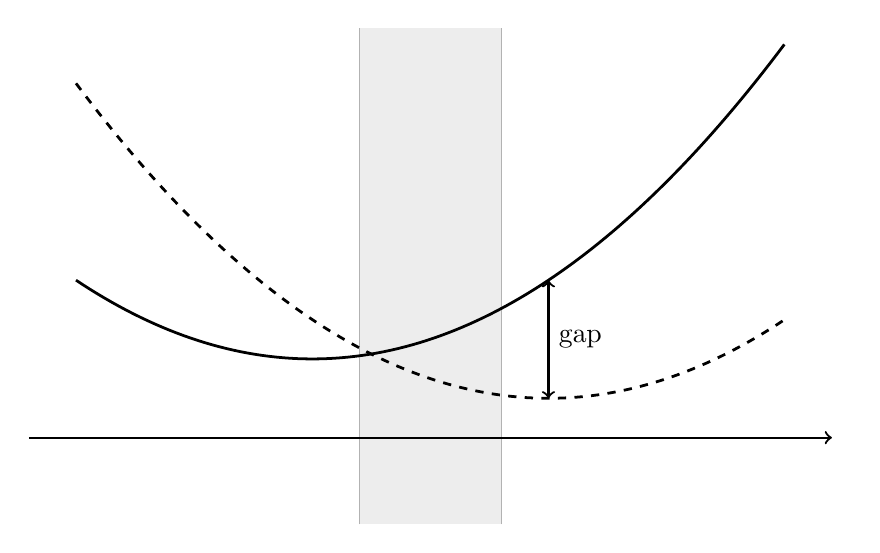
\begin{tikzpicture}[x=3cm, y=1cm]
			% --- editable bounds for the vertical strip (hypothesis space) ---
  			\def\hmin{0.2}   % left x-bound of \mathcal{H}
  			\def\hmax{0.8}   % right x-bound of \mathcal{H}
  			\def\ymin{-2.1}  % lower y-bound (should cover your plot)
  			\def\ymax{4.2}   % upper y-bound (should cover your plot)
  			% Hypothesis space: vertical grey, semi-transparent strip
  			\fill[gray!40, opacity=0.35] (\hmin,\ymin) rectangle (\hmax,\ymax);
  			% (optional) faint borders for the strip
  			\draw[gray!60] (\hmin,\ymin) -- (\hmin,\ymax);
  			\draw[gray!60] (\hmax,\ymin) -- (\hmax,\ymax);
  			% Label for the strip
  			\node[rotate=0] at ({(\hmin+\hmax)/2}, {\ymax-0.2}) {$\hypospace$};
			\node[anchor=west] at (2, 4) {$\risk{\hypothesis}$};
			\draw[line width=1, domain=-2:1, samples=100,dashed] plot  ({\x+1}, {\x*\x -0.5}) node[right] {$\emprisk{\dataset}{\hypothesis}$};
			\draw[line width=1, domain=-1:2, samples=100] plot ({\x}, {\x*\x});
			\draw[<->, thick] (1, -0.5) -- (1, 1) node[midway, right] {gap};
			% Horizontal axis for hypothesis variable
            		\draw[->, thick] (-1.2,-1) -- (2.2,-1) node[below right] {$\hypothesis$};
			\end{tikzpicture}
			\end{center}
		\caption{The \gls{generalization} gap can be defined as 
			the difference between the 
			\gls{risk} $\risk{\hypothesis}$ and the average \gls{loss} (or \gls{emprisk}) 
			$\emprisk{\hypothesis}{\trainset}$ computed on a \gls{trainset}.}
		\end{figure}
	  	In practice, the \gls{probdist} underlying this \gls{expectation} is 
	  	unknown. Thus, we need to estimate the \gls{expectation} based on 
	  	observed \glspl{datapoint}. \Gls{validation} techniques 
	  	use different constructions of a \gls{valset}, which is different from 
	  	the \gls{trainset}, to estimate the \gls{generalization} gap.
		\\
		See also: \gls{generalization}, \gls{validation}, \gls{erm}, \gls{lossfunc}.}, 
	first={generalization gap}, 
	text={generalization gap}
}

\newglossaryentry{lda} 
{name={linear discriminant analysis (LDA)}, 
	description={LDA\index{linear discriminant analysis (LDA)} is a classical 
         	\gls{featlearn} method \cite{BishopBook}, \cite{Fisher1936Taxonomic}. 
		In the context of \gls{binclass} problems, 
		LDA seeks a linear \gls{featuremap} $\featuremap^{(\weights)}: \mathbb{R}^{\nrfeatures} 
		\rightarrow \mathbb{R}: \featurevec \mapsto \weights^{T} \featurevec$ 
		such that the new \gls{feature} $\featuremap^{(\weights)}(\featurevec)$ 
		optimally allows us to predict the \gls{label} of a \gls{datapoint}. 
		\\
		See also: \gls{featlearn}, \gls{dimred}, \gls{selfsupervisedlearning}. }, 
 	first={linear discriminant analysis (LDA)},
 	text={LDA}, 
 	firstplural={linear discriminant analyses (LDAs)},
 	plural={LDAs}
}

\newglossaryentry{randomprojection} 
{name={random projection}, 
	description={A random \gls{projection}\index{random projection} uses a random \gls{widematrix} 
		$\mathbf{A}\!\in\!\mathbb{R}^{\nrfeatures' \times \nrfeatures}$, with 
		$\nrfeatures' < \nrfeatures$, to map a \gls{featurevec} 
		$\featurevec \!\in\! \mathbb{R}^{\nrfeatures}$ to a shorter 
		\gls{featurevec} $\mathbf{A}\featurevec \!\in\! \mathbb{R}^{\nrfeatures'}$. 
		It is a basic method for \gls{featlearn} and \gls{dimred}. 
		The \gls{projection} \gls{matrix} $\mathbf{A}$ is typically generated entrywise 
		by \gls{iid} \glspl{rv} with a common \gls{probdist} $\probdist$. 
		For a broad class of such \glspl{probdist}, a random \gls{projection} 
		approximately preserves pairwise \glspl{eucliddist} between \glspl{featurevec} 
		of a given finite \gls{dataset}. The celebrated \gls{johnsonlindenstrausslemma} 
		guarantees the existence of such a distance-preserving \gls{dimred} \gls{map} 
		but does not itself involve randomness. Random \glspl{projection} provide a 
		probabilistic construction that realizes this guarantee with high \gls{probability}. 
		Roughly speaking, for many relevant applications, random \glspl{projection} 
		preserve the most relevant information contained in the original (typically 
		very long) \gls{featurevec}. Fig.~\ref{fig:randomprojection_dict} illustrates this 
		behavior for an RGB image. The left panel shows the original image. The middle panel 
		shows a masked image where a randomly selected five percent of the original pixels are kept, and 
		the remaining pixels are set to a fixed light-gray color. The right panel shows the result of a 
		simple reconstruction based on repeated averaging of nearby retained pixels. 
		\begin{figure}[H]
			\centering
			\begin{minipage}[t]{0.32\textwidth}
				\includegraphics[width=\linewidth]{assets/pythonsnacks/randomprojection/randomprojection_original.png}
				\caption*{original}
				\vspace{2ex}
				\centering
				{\selectfont (a)}
			\end{minipage}\hfill
			\begin{minipage}[t]{0.32\textwidth}
				\includegraphics[width=\linewidth]{assets/pythonsnacks/randomprojection/randomprojection_masked.png}
				\caption*{95 \% masked}
				\vspace{2ex}
				\centering
				{\selectfont (b)}
			\end{minipage}\hfill
			\begin{minipage}[t]{0.32\textwidth}
				\includegraphics[width=\linewidth]{assets/pythonsnacks/randomprojection/randomprojection_reconstructed.png}
				\caption*{reconstructed}
				\vspace{2ex}
				\centering
				{\selectfont (c)}
			\end{minipage}
		\caption{Illustration of a random \gls{projection} in the form of removing (or masking) 
			all image pixels, except those in a small random subset. 
			(a) The left panel shows the original RGB image. (b) The middle panel shows a version 
			with only a random five percent subset of pixels retained. (c) The right panel shows a 
			simple convolution-based reconstruction that diffuses information from 
			the known pixels into masked regions.}
			\label{fig:randomprojection_dict}
		\end{figure}
		See also: \gls{featlearn}, \gls{dimred}, \gls{johnsonlindenstrausslemma}. 
		\\
		Python demo: \href{https://github.com/AaltoDictionaryofML/AaltoDictionaryofML.github.io/blob/main/assets/pythonsnacks/randomprojection/randomprojection.py}{click me}},
	first={random projection},
	plural={random projections}, 
	firstplural={random projections}, 
	text={random projection}
}

\newglossaryentry{boosting}
{name={boosting}, 
	description={Boosting\index{boosting} is an iterative \gls{optmethod} to learn 
		an accurate \gls{hypothesis} \gls{map} (or strong learner) by sequentially 
		combining less accurate \glspl{baselearner} (referred to as weak learners) 
		\cite{pmlr-vR2-ridgeway99a}, \cite{Schapire1999}, \cite{Drucker1997}, \cite[Ch. 10]{hastie01statisticallearning}.
		Boosting can be understood as a \gls{generalization} of \glspl{gdmethod} 
		for \gls{erm} using \glspl{parammodel} and \gls{smooth} \glspl{lossfunc} 
		\cite{Friedman2001}. In particular, starting from an initialization $\widetilde{\hypothesis}$, 
		boosting methods construct a \gls{sequence} of \glspl{hypothesis} 
		$\widetilde{\hypothesis}^{(\iteridx)}$, $\iteridx=1,\,\ldots$, 
		via a generalized \gls{gradstep} 
		$$ \widetilde{\hypothesis}^{(\iteridx)} = \widetilde{\hypothesis}^{(\iteridx-1)}+
		\lrate^{(\iteridx)} 
		\learnthypothesis^{(\iteridx)}.$$ 
		Here, $\lrate^{(\iteridx)}$ denotes a \gls{learnrate} and 
		$\learnthypothesis^{(\iteridx)}$ is provided 
		by the $\iteridx$th \gls{baselearner}. Comparing the above update with the 
		plain \gls{gradstep} suggests that we view $\learnthypothesis^{(\iteridx)}$ 
		as a (negative) generalized \gls{gradient}. 
		Boosting methods differ in their choice of \glspl{baselearner} for computing 
		the generalized \glspl{gradient} $\learnthypothesis^{(\iteridx)}$. 
		\begin{figure}[H]
			\begin{center}
				\begin{tikzpicture}[scale=1.2]
					% Axes
					\draw[->] (-0.5,0) -- (5.5,0) node[right] {$\hypothesis$};
					\draw[->] (0,-0.5) -- (0,4.5) node[above] {$\emprisk{\hypothesis}{\dataset}$};
					\draw[thick,domain=0.2:5,smooth,variable=\x,blue!60] plot ({\x},{(4 - 1.3*\x + 0.15*\x*\x)});
					\foreach \x/\label in {0.7/$\widetilde{\hypothesis}^{(0)}$, 1.5/$\widetilde{\hypothesis}^{(1)}$, 2.3/$\widetilde{\hypothesis}^{(2)}$, 3.0/$\widetilde{\hypothesis}^{(3)}$} {
						\draw[dashed, gray] (\x, 0) -- (\x, {4 - 1.3*\x + 0.15*\x*\x}); % helper line
						\filldraw[black] (\x, {4 - 1.3*\x + 0.15*\x*\x}) circle (2pt);   % point
						\node[below] at (\x, -0.1) {\label};                             % label
					}
				\end{tikzpicture}
			\end{center} 
		\caption{Boosting methods construct a \gls{sequence} of \gls{hypothesis} \glspl{map} 
			via a generalized \gls{gradstep}. This generalized \gls{gradstep} uses the \gls{output} of 
			\glspl{baselearner}.\label{fig_boosting_dict}}
     		\end{figure} 
     		See also: \gls{ensemble}, \gls{adaboost}, \gls{gradientboosting}.}, 
	first={boosting}, 
	text={boosting}
} 

\newglossaryentry{mse} 
{name={mean squared error (MSE)}, 
	description={The MSE\index{mean squared error (MSE)} of a \gls{hypothesis} 
         	is the average \gls{sqerrloss} computed over a given \gls{dataset}. 
               	In theoretical analyses, MSE also denotes the expected \gls{sqerrloss}, 
               	i.e., the corresponding \gls{risk}.
		\\ 
		See also: \gls{sqerrloss}, \gls{risk}.}, 
 	first={mean squared error (MSE)}, 
 	text={MSE}
}

\newglossaryentry{mae} 
{name={mean absolute error (MAE)}, 
	description={The MAE\index{mean absolute error (MAE)} of a \gls{hypothesis} 
        		is the average \gls{abserr} computed over a given \gls{dataset}. 
               	In theoretical analyses, MAE also denotes the expected \gls{abserr}, 
               	i.e., the corresponding \gls{risk}.
		\\ 
		See also: \gls{abserr}, \gls{risk}.}, 
 	first={mean absolute error (MAE)}, 
 	text={MAE}
}

\newglossaryentry{adaboost}
{name={adaptive boosting (AdaBoost)},
	description={AdaBoost\index{adaptive boosting (AdaBoost)} is a specific 
		\gls{boosting} \gls{algorithm} that combines \glspl{baselearner} sequentially 
		\cite{pmlr-vR2-ridgeway99a}, \cite{Schapire1999}, \cite{Drucker1997}. 
	    	The core idea of AdaBoost is to use the \gls{prediction} errors of the current  
		\gls{baselearner} for \gls{sampleweighting} in the next \gls{baselearner}. 
		In particular, the $\iteridx$th \gls{baselearner} learns a \gls{hypothesis} 
		$\learnthypothesis^{(\iteridx)}$ by weighted \gls{erm} with  
		\gls{sample} \glspl{weight} $\sampleweight{\sampleidx}$. The \gls{prediction} errors of 
		$\learnthypothesis^{(\iteridx)}$ are then used to update the 
		\gls{sample} \glspl{weight} by increasing the \glspl{weight} of \glspl{datapoint} 
		that have been predicted poorly (i.e., with large \gls{loss}) 
		by $\learnthypothesis^{(\iteridx)}$. The updated \gls{sample} \glspl{weight} are 
		then used in the next \gls{baselearner} to learn $\learnthypothesis^{(\iteridx+1)}$. 
		The ultimate \gls{hypothesis} $\widetilde{\hypothesis}^{(\nriter)}$ delivered after 
		$\nriter$ \glspl{iteration} is a linear combination of the \glspl{hypothesis} 
		$\learnthypothesis^{(1)},\,\ldots,\,\learnthypothesis^{(\nriter)}$. 
		AdaBoost can be interpreted as a generalized \gls{gradstep} \cite[Ch. 10.4]{hastie01statisticallearning}
		$$\widetilde{\hypothesis}^{(\iteridx)}=\widetilde{\hypothesis}^{(\iteridx-1)}+\lrate^{(\iteridx)} \learnthypothesis^{(\iteridx)}.$$   
		This generalized \gls{gradstep} involves a \gls{learnrate} $\lrate^{(\iteridx)}$, which 
		controls the amount of modification of the current \gls{hypothesis}. 
		\\
		See also: \gls{boosting}, \gls{sampleweighting}, \gls{erm}.}, 
	first={adaptive boosting (AdaBoost)}, 
	text={AdaBoost}
}

\newglossaryentry{gradientboosting}
{name={gradient boosting},
 	description={\Gls{gradient} \gls{boosting}\index{gradient boosting} is a \gls{boosting} 
 		\gls{algorithm} that learns a \gls{hypothesis} $\widetilde{\hypothesis}$ 
 		by sequentially combining the \glspl{hypothesis} $\learnthypothesis^{(\iteridx)}$ 
 		\cite[Algorithm 10.3]{hastie01statisticallearning}, \cite{Friedman2001}. 
 		Similar to \gls{adaboost}, \gls{gradient} \gls{boosting} uses a generalized \gls{gradstep} 
 		to combine the results of the \glspl{baselearner}:
        		$$\widetilde{\hypothesis}^{(\iteridx)} = \widetilde{\hypothesis}^{(\iteridx-1)}-\lrate^{(\iteridx)} 
 		\learnthypothesis^{(\iteridx)},$$
 		where the generalized \gls{gradient} $\learnthypothesis{\iteridx}$ is constructed from 
		the $\iteridx$th \gls{baselearner}.
 		The difference between \gls{adaboost} and \gls{gradient} \gls{boosting} is in the construction 
		of $\learnthypothesis{\iteridx}$. While \gls{adaboost} uses weighted \gls{erm} for this construction, 
		\gls{gradient} \gls{boosting} uses \gls{erm} on a modified \gls{trainset}. This modification is obtained 
		by leaving the \glspl{featurevec} untouched but replacing the \glspl{label} with the 
		\gls{partialderivative} of the \gls{lossfunc} with respect to the \glspl{prediction} 
		of the previous \gls{baselearner}.   
 		 \\
 		See also: \gls{boosting}, \gls{adaboost}, \gls{gd}.},
 	first={gradient boosting}, 
 	text={gradient boosting}
}
	
\newglossaryentry{gtv}
{name={generalized total variation (GTV)}, 
	description={GTV is a\index{generalized total variation (GTV)} 
		\gls{measure} of the variation of trained \glspl{localmodel} $\localhypothesis{\nodeidx}$ 
		(or their \glspl{modelparam} $\localparams{\nodeidx}$) assigned to the nodes $\nodeidx=1, \,\ldots, \,\nrnodes$ 
		of an undirected weighted \gls{graph} $\graph$ with edges $\edges$. Given a \gls{measure} $\discrepancy{\hypothesis}{\hypothesis'}$ 
		of the \gls{discrepancy} between \gls{hypothesis} \glspl{map} $\hypothesis,\hypothesis'$, the GTV is 
		\begin{equation} 
			\nonumber
			\sum_{\edge{\nodeidx}{\nodeidx'}\in \edges} \edgeweight_{\nodeidx,\nodeidx'} 
			\discrepancy{\localhypothesis{\nodeidx}}{\localhypothesis{\nodeidx'}}.
		\end{equation}
		Here, $\edgeweight_{\nodeidx,\nodeidx'}>0$ denotes the weight of the undirected edge $\edge{\nodeidx}{\nodeidx'}\in \edges$.
				\\
		See also: \gls{localmodel}, \gls{modelparam}, \gls{graph}, \gls{discrepancy}, \gls{hypothesis}, \gls{map}.},
	first={generalized total variation (GTV)},
	text={GTV} 
}
	
\newglossaryentry{srm}
{name={structural risk minimization (SRM)}, 
	description={SRM\index{structural risk minimization (SRM)} is an
		instance of \gls{rerm} with which the \gls{model} $\hypospace$ can be expressed 
		as a \gls{countable} union of submodels such that $\hypospace = \bigcup_{n=1}^{\infty} \hypospace^{(n)}$. 
		Each submodel $\hypospace^{(n)}$ permits the derivation of an approximate upper bound 
		on the \gls{generalization} error incurred when applying \gls{erm} to train $\hypospace^{(n)}$. 
		These individual bounds—one for each submodel—are then combined to form a \gls{regularizer} 
		used in the \gls{rerm} objective. 
        		These approximate upper bounds (one for each $\hypospace^{(n)}$) are then combined 
		to construct a \gls{regularizer} for \gls{rerm} \cite[Sec.\ 7.2]{ShalevMLBook}.
				\\
		See also: \gls{rerm}, \gls{model}, \gls{generalization}, \gls{erm}, \gls{regularizer}, \gls{risk}.},
	first={structural risk minimization (SRM)},
	text={SRM}
}

\newglossaryentry{rlm}
{name={regularized loss minimization (RLM)},
 	description={See\index{regularized loss minimization (RLM)} \gls{rerm}.},
	first={regularized loss minimization (RLM)}, 
 	text={RLM}
} 

\newglossaryentry{datapoisoning}
{name={data poisoning}, 
	description={\Gls{data}\index{data poisoning} poisoning refers to the intentional 
		manipulation (or fabrication) of \glspl{datapoint} to maliciously 
		steer the \gls{training} of an \gls{ml} \gls{model} \cite{Liu2021}, \cite{PoisonGAN}. 
  		\Gls{data} poisoning \glspl{attack} take various forms, including 
		\gls{backdoor} and \glspl{dosattack}. A \gls{backdoor} \gls{attack} 
		implants triggers into \gls{training} \gls{data}, so that the trained \gls{model} 
		behaves normally for typical \glspl{datapoint} but misclassifies a 
		\gls{datapoint} with a \gls{featurevec} that contains a trigger pattern.
  		A \gls{dosattack} degrades the trained \gls{model}'s overall performance 
		by injecting mislabeled or adversarial examples to prevent effective learning.
		\Gls{data} poisoning is particularly harmful in decentralized or 
		distributed \gls{ml} settings (such as \gls{fl}), where \gls{training} 
		\gls{data} cannot be centrally verified.
				\\
		See also: \gls{attack}, \gls{backdoor}, \gls{dosattack}, \gls{trustAI}.},
	first={data poisoning},
	text={data poisoning} 
}
	
\newglossaryentry{backdoor}
{name={backdoor}, 
 	description={A\index{backdoor} backdoor \gls{attack} refers to the intentional 
 		manipulation of an \gls{ml} \gls{training} process. The attacker 
 		might perturb the \gls{trainset} (i.e., through \gls{datapoisoning}) 
 		or the \gls{optmethod} used by an \gls{erm}-based method. 
 		The goal of a backdoor \gls{attack} is to nudge the learned \gls{hypothesis} $\learnthypothesis$ 
 		toward specific \glspl{prediction} for a certain subset $\mathcal{T} \subset \featurespace$ 
 		of the \gls{featurespace}. Any \gls{featurevec} $\featurevec \in \mathcal{T}$ 
 		serves as a key (or trigger) to unlock a backdoor, in the sense of delivering 
 		anomalous \glspl{prediction}. The 
 		trigger pattern $\mathcal{T}$ and corresponding anomalous \gls{prediction} 
 		$\learnthypothesis(\featurevec)$, for $\featurevec \in \mathcal{T}$, 
 		are only known to the attacker.
 				\\
 		See also: \gls{attack}, \gls{datapoisoning}.},
 	first={backdoor},
 	text={backdoor} 
}

\newglossaryentry{clustasspt}
{name={clustering assumption}, 
	description={The\index{clustering assumption} 
		\gls{clustering} assumption postulates that \glspl{datapoint} in a \gls{dataset} form a (small) number of 
		groups or \glspl{cluster}. \Glspl{datapoint} in the same \gls{cluster} are more similar to each 
		other than those outside the \gls{cluster} \cite{SemiSupervisedBook}. We obtain different 
		\gls{clustering} methods by using different notions of similarity between \glspl{datapoint}.
				\\
		See also: \gls{clustering}, \gls{datapoint}, \gls{dataset}, \gls{cluster}.},
	first={clustering assumption},
	text={clustering assumption} 
}
	
\newglossaryentry{dosattack}
{name={denial-of-service attack},
	description={A\index{denial-of-service attack} 
		denial-of-service \gls{attack} aims (e.g., via \gls{datapoisoning}) to steer the \gls{training} of a \gls{model} 
		such that it performs poorly for typical \glspl{datapoint}.
				\\
		See also: \gls{attack}, \gls{datapoisoning}, \gls{model}, \gls{datapoint}.},
	first={denial-of-service attack},
	plural={denial-of-service attacks},
	firstplural={denial-of-service attacks},
	text={denial-of-service attack} 
}

\newglossaryentry{netexpfam}
{name={networked exponential families (nExpFam)}, 
	description={nExpFam is a\index{networked exponential families (nExpFam)} collection of exponential 
		families, each of them assigned to a node of an \gls{flnetwork}. The \glspl{modelparam} are coupled 
	   	via the network structure by requiring them to have a small \gls{gtv} \cite{JungNetExp2020}.
	   		\\
		See also: \gls{flnetwork}, \gls{modelparam}, \gls{gtv}.},
	first={networked exponential family (nExpFam)},
	text={nExpFam} 
}

\newglossaryentry{scatterplot}
{name={scatterplot}, 
	description={A\index{scatterplot} 
		visualization technique that depicts \glspl{datapoint} using markers in a 2-D plane. 
		Fig. \ref{fig_scatterplot_temp_FMI_dict} depicts an example of a scatterplot.  
		\begin{figure}[H]
			\begin{center}
				\begin{tikzpicture}[scale=1]
					\tikzset{x=2cm,y=2cm,every path/.style={>=latex},node style/.style={circle,draw}}
					\begin{axis}[axis x line=none,
						axis y line=none,
						ylabel near ticks,
						xlabel near ticks,
						enlarge y limits=true,
						xmin=-5, xmax=30,
						ymin=-5, ymax=30,
						width=6cm, height=6cm ]
						\addplot[only marks] table [x=mintmp, y=maxtmp, col sep = semicolon] {assets/FMIData1.csv};
						\node at (axis cs:26,2) [anchor=west] {$\feature$};
						\node at (axis cs:0,30) [anchor=west] {$\truelabel$};
						\draw[->] (axis cs:-5,0) -- (axis cs:30,0);
						\draw[->] (axis cs:0,-5) -- (axis cs:0,30);
					\end{axis}
				\end{tikzpicture}
				\vspace*{-10mm}
			\end{center}
		\caption{A scatterplot with circle markers, where the \glspl{datapoint} represent daily weather conditions in Finland. 
			Each \gls{datapoint} is characterized by its \gls{minimum} daytime temperature $\feature$ 
			as the \gls{feature} and its \gls{maximum} daytime temperature $\truelabel$ as the \gls{label}. 
			The temperatures have been measured at the \gls{fmi} weather station Helsinki Kaisaniemi 
			during 1 September 2024—28 October 2024.}
			\label{fig_scatterplot_temp_FMI_dict}
			\vspace*{-3mm}
		\end{figure}
		A scatterplot can enable the visual inspection of \glspl{datapoint} that are naturally 
		represented by \glspl{featurevec} in high-dimensional spaces.
		\\
		See also: \gls{datapoint}, \gls{minimum}, \gls{feature}, \gls{maximum}, \gls{label}, \gls{fmi}, \gls{featurevec}, \gls{dimred}.},
	first={scatterplot},
	text={scatterplot} 
}

\newglossaryentry{stepsize}
{name={step size}, 
	description={See\index{step size} \gls{learnrate}.}, 
	first={step size},
	text={step size} 
}

\newglossaryentry{learnrate}
{name={learning rate}, 
	description={Consider\index{learning rate} an iterative \gls{ml} method for finding or 
	    	learning a useful \gls{hypothesis} $\hypothesis \in \hypospace$. 
		Such an iterative method repeats similar computational (update) steps that adjust or 
		modify the current \gls{hypothesis} to obtain an improved \gls{hypothesis}. 
		A key \gls{parameter} of an iterative method is the learning rate. The learning rate 
		controls the extent to which the current \gls{hypothesis} can be modified during a 
		single \gls{iteration}. Consider, for example, the \gls{gradstep} \cite[Ch. 5]{MLBasics} 
		\begin{equation}
			\label{equ_def_basic_gradstep_lrate_dict}
			\weights^{(\iteridx\!+\!1)} = \weights^{(\iteridx)} - \lrate \nabla f(\weights^{(\iteridx)})
       		\end{equation} 
		of a \gls{gdmethod} for \gls{erm}, where the \gls{objfunc} $f(\weights)$ 
		is the \gls{emprisk} incurred by $\hypothesis^{(\weights)}$ on a \gls{trainset}. 
		Given the current \glspl{modelparam} $\weights^{(\iteridx)}$ at \gls{iteration} $\iteridx$, 
		the \gls{gradstep} produces updated \glspl{modelparam} $\weights^{(\iteridx\!+\!1)}$ 
		by moving in the opposite direction of the \gls{gradient} $\nabla f(\weights^{(\iteridx)})$. 
		\begin{figure}[H]
			\begin{center}
			\begin{minipage}{0.45\columnwidth}
			\begin{tikzpicture}[xscale=0.4,yscale=0.6]
				\draw[blue, ultra thick, domain=-4.1:4.1] plot (\x,  {(1/4)*\x*\x});
				\draw[] (1,0.25) circle [radius=0.1] node [right] (A) {$f(\weights^{(\iteridx)})$} ;
				\draw[] (-2,1) circle [radius=0.1] node [left] (B) {$f(\weights^{(\iteridx\!+\!1)})$} ;
				\draw[] (3,2.25) circle [radius=0.1]  node  [right] (C) {$f(\weights^{(\iteridx\!+\!2)})$} ;
				\draw[->,dashed] (-2,1) -- (3,2.25) node [midway,above] {\eqref{equ_def_basic_gradstep_lrate_dict}};
				\draw[->,dashed]  (1,0.25) -- (-2,1) node [midway,above] {\eqref{equ_def_basic_gradstep_lrate_dict}};
				\node [below] at (0,-0.2) {(a)};
			\end{tikzpicture}
			\end{minipage}
			\begin{minipage}{0.45\columnwidth}
			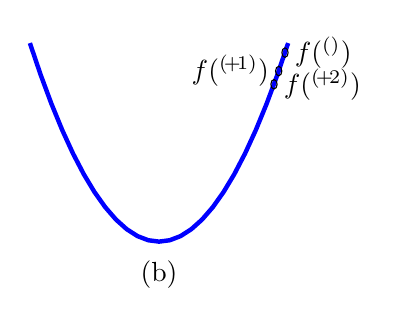
\begin{tikzpicture}[xscale=0.4,yscale=0.6]
				\draw[blue, ultra thick, domain=-4.1:4.1] plot (\x,  {(1/4)*\x*\x});
				\draw[] (4,4) circle [radius=0.1];
				\node [right] at (4,4) {$f(\weights^{(\iteridx)})$};
				\draw[] (3.8,3.61) circle [radius=0.1];
				\node [left] at (3.8,3.61) {$f(\weights^{(\iteridx\!+\!1)})$};
				\draw[] (3.65,3.33) circle [radius=0.1];
				\node [right] at (3.65,3.33) {$f(\weights^{(\iteridx\!+\!2)})$};
				\node [below] at (0,-0.2) {(b)};
			\end{tikzpicture}
			\end{minipage}
			\end{center}
		\caption{Effect of using an inadequate learning rate $\lrate$ in the \gls{gradstep} 
			\eqref{equ_def_basic_gradstep_lrate_dict}. (a) If $\lrate$ is too large, 
			the \glspl{gradstep} can ``overshoot'' such that the iterates $\weights^{(\iteridx)}$ 
			diverge away from the optimum, i.e., $f(\weights^{(\iteridx\!+\!1)}) > f(\weights^{(\iteridx)})$. 
			(b) If $\lrate$ is too small, the \glspl{gradstep} make too little progress towards 
			the optimum within the available number of \glspl{iteration} (due to limited computational budget). 
			\label{fig_small_large_lrate_dict}}
		\end{figure}
		See also: \gls{ml}, \gls{hypothesis}, \gls{parameter}, \gls{gd}, \gls{stochGD}, \gls{projgd}, \gls{stepsize}.},
	first={learning rate},
	text={learning rate} 
}

\newglossaryentry{featuremap}
{name={feature map}, 
	description={A \gls{feature} \gls{map}\index{feature map} refers to a \gls{function} 
		$$
		\featuremapvec: \featurespace \rightarrow \featurespace', \qquad \featurevec \mapsto \featurevec'
		$$
		that transforms a \gls{featurevec} $\featurevec \in \featurespace$ of 
 		a \gls{datapoint} into a new \gls{featurevec} $\featurevec' \in \featurespace'$, 
 		where $\featurespace'$ is typically different from $\featurespace$.
 		The transformed representation $\featurevec'$ is often more useful than the original 
 		$\featurevec$. For instance, the geometry of \glspl{datapoint} may become more linear 
 		in $\featurespace'$, allowing the application of a \gls{linmodel} to $\featurevec'$. 
 		This idea is central to the design of \glspl{kernelmethod}~\cite{LearningKernelsBook}.
 		Other benefits of using a \gls{feature} \gls{map} include reducing \gls{overfitting} and 
 		improving \gls{interpretability}~\cite{Ribeiro2016}. A common use case is \gls{data} 
 		visualization, where a \gls{feature} \gls{map} with two output dimensions allows the representation 
 		of \glspl{datapoint} in a 2-D \gls{scatterplot}. Some \gls{ml} methods employ trainable 
 		\gls{feature} \glspl{map}, whose \glspl{parameter} are learned from \gls{data}. An example is 
 		the use of hidden \glspl{layer} in a \gls{deepnet}, which act as successive \gls{feature} \glspl{map} 
 		\cite{MallatUnderstandingDeepLearning}. A principled way to train a \gls{feature} \gls{map} 
 		is through \gls{erm}, using a \gls{lossfunc} that measures reconstruction quality, 
 		e.g., $\lossfun = \|\featurevec - r(\featurevec')\|^2$, where $r(\cdot)$ is a trainable
 		\gls{map} that attempts to reconstruct $\featurevec$ from the transformed \gls{featurevec} $\featurevec'$.
				\\
		See also: \gls{feature}, \gls{map}, \gls{kernelmethod}, \gls{featlearn}, \gls{pca}.},
	first={feature map},
	text={feature map} 
}
 
\newglossaryentry{lasso}
{name={least absolute shrinkage and selection operator (Lasso)}, 
	description={The Lasso \index{least absolute shrinkage and selection operator (Lasso)} is an 
		instance of \gls{eerm} \cite{hastie01statisticallearning}. It learns the \glspl{weight} 
		$\weights$ of a \gls{linearmap} $\hypothesis(\featurevec) = \weights\,^{T} \featurevec$ from a \gls{trainset}. 
		Lasso is obtained from \gls{linreg} by adding the scaled $\ell_{1}$-\gls{norm} 
		$\regparam \normgeneric{\weights}{1}$ to the average \gls{sqerrloss} incurred on 
		the \gls{trainset} \cite{Tibshirani1996}. Using the $\ell_{1}$-\gls{norm} as a \gls{regularizer}, 
		instead of the squared $\ell_{2}$-\gls{norm} used in \gls{ridgeregression}, encourages the 
		learned \glspl{weight} to have many entries set to zero \cite{Wain2019}, \cite{BuhlGeerBook}.
				\\
		See also: \gls{eerm}, \gls{weight}, \gls{linearmap}, \gls{trainset}, \gls{linreg}, \gls{norm}, \gls{sqerrloss}.},
	first={Lasso},
	text={Lasso} 
}
 
\newglossaryentry{simgraph}
{name={similarity graph}, 
 	description={Some\index{similarity graph} \gls{ml} applications generate \glspl{datapoint} that 
 		are related by a domain-specific notion of similarity. These similarities can be 
 		represented conveniently using a similarity \gls{graph} $\graph = \big(\nodes \defeq \{1, \,\ldots, \,\samplesize\}, \edges\big)$. 
 		The node $\sampleidx \in \nodes$ represents the $\sampleidx$th \gls{datapoint}. Two 
 		nodes are \gls{connected} by an undirected edge if the corresponding \glspl{datapoint} are similar. 
				\\
		See also: \gls{ml}, \gls{datapoint}, \gls{graph}, \gls{connected}.},
 	first={similarity graph},
	text={similarity graph} 
}

\newglossaryentry{kernel}
{name={kernel (kernel method)}, 
	description={Consider\index{kernel (kernel method)} a set of \glspl{datapoint}, each represented by a \gls{featurevec} 
	 	$\featurevec \in \featurespace$, where $\featurespace$ denotes the \gls{featurespace}. 
	 	A (real-valued) kernel is a \gls{function} 
	 	$\kernel: \featurespace \times \featurespace \rightarrow \mathbb{R}$ that assigns to every pair of 
     		\glspl{featurevec} $\featurevec, \featurevec' \in \featurespace$ a real number $\kernelmap{\featurevec}{\featurevec'}$. 
     		This value is typically interpreted as a similarity \gls{measure} between $\featurevec$ and $\featurevec'$. 
	 	The defining property of a kernel is that it is symmetric, i.e.,
	 	$\kernelmap{\featurevec}{\featurevec'} = \kernelmap{\featurevec'}{\featurevec}$, and that 
	 	for any finite set of \glspl{featurevec} $\featurevec_1, \,\ldots, \,\featurevec_n \in \featurespace$, the \gls{matrix} 
	  	\begin{equation}
	 		\nonumber
	 		\mathbf{K} = \begin{pmatrix}
	 			\kernelmap{\featurevec_1}{\featurevec_1} & \kernelmap{\featurevec_1}{\featurevec_2} & \ldots & \kernelmap{\featurevec_1}{\featurevec_n} \\
	 			\kernelmap{\featurevec_2}{\featurevec_1} & \kernelmap{\featurevec_2}{\featurevec_2} & \ldots & \kernelmap{\featurevec_2}{\featurevec_n} \\
	 			\vdots											
	 			& \vdots & \ddots & \vdots \\
	 			\kernelmap{\featurevec_n}{\featurevec_1} & \kernelmap{\featurevec_n}{\featurevec_2} & \ldots & \kernelmap{\featurevec_n}{\featurevec_n} 
	 		\end{pmatrix} \in \mathbb{R}^{n \times n}
	 	\end{equation}
	 	is \gls{psd}. 
     		A kernel naturally defines a transformation of a \gls{featurevec} $\featurevec$ into a 
	 	\gls{function} $\vz = \kernelmap{\featurevec}{\cdot}$. The \gls{function} $\vz$ maps an  
	 	input $\featurevec' \in \featurespace$ to the value $\kernelmap{\featurevec}{\featurevec'}$. 
	 	We can view the \gls{function} $\vz$ as a new \gls{featurevec} that belongs to a 
	 	\gls{featurespace} $\featurespace'$ that is typically different from $\featurespace$. 
	 	This new \gls{featurespace} $\featurespace'$ has a particular mathematical structure, i.e., it is a 
	 	reproducing kernel \gls{hilbertspace} (RKHS)~\cite{LearningKernelsBook}, \cite{LampertNowKernel}.
     		Since $\vz$ belongs to a RKHS, which is a \gls{vectorspace}, we can interpret it as a generalized 
	 	\gls{featurevec}. Note that a finite-length \gls{featurevec} $\featurevec=\big(\feature_{1}, \,\ldots, \,\feature_{\nrfeatures} \big)\,^{T} \in \mathbb{R}^{\nrfeatures}$ 
	 	can be viewed as a \gls{function} $\featurevec: \{1, \,\ldots, \,\nrfeatures\} \rightarrow \mathbb{R}$ 
	 	that assigns a real value to each index $\featureidx \in \{1, \,\ldots, \,\nrfeatures\}$.
          		\\
		See also: \gls{featurevec}, \gls{featurespace}, \gls{hilbertspace}, \gls{kernelmethod}.},
	first={kernel},
	text={kernel} 
}
	
\newglossaryentry{kernelmethod}
{name={kernel method},
	description={A\index{kernel method} \gls{kernel} method is an \gls{ml} method that uses a 
		\gls{kernel} $\kernel$ to map the original (i.e., raw) \gls{featurevec} $\featurevec$ of a 
		\gls{datapoint} to a new (transformed) \gls{featurevec} $\vz = \kernelmap{\featurevec}{\cdot}$ \cite{LearningKernelsBook}, \cite{LampertNowKernel}.
		The motivation for transforming the \glspl{featurevec} is that, by using a suitable \gls{kernel}, 
		the \glspl{datapoint} have a more "pleasant" geometry in the transformed \gls{featurespace}. 
		For example, in a \gls{binclass} problem, using transformed \glspl{featurevec} $\vz$ might 
		allow us to use \glspl{linmodel}, even if the \glspl{datapoint} are not linearly 
		separable in the original \gls{featurespace} (see Fig. \ref{fig_linsep_kernel_dict}). 
		\begin{figure}[H]
			\begin{center}
 			\begin{tikzpicture}[auto,scale=0.6]
        			% Left rectangle (\featurespace)
       			% \draw [thick] (-9,-3) rectangle (-2,4) node [anchor=east,above] {$\featurespace$};
        			\draw [thick] (-6,2) circle (0.1cm) node[anchor=west] {\hspace*{0mm}$\featurevec^{(5)}$};
       			\draw [thick] (-8,1.6) circle (0.1cm) node[anchor=west] {\hspace*{0mm}$\featurevec^{(4)}$};
        			\draw [thick] (-7.4,-1.7) circle (0.1cm) node[anchor=west] {\hspace*{0mm}$\featurevec^{(3)}$};
        			\draw [thick] (-6,-1.9) circle (0.1cm) node[anchor=west] {\hspace*{0mm}$\featurevec^{(2)}$};
        			\draw [thick] (-6.5,0.0) rectangle ++(0.1cm,0.1cm) node[anchor=west,above] {\hspace*{0mm}$\featurevec^{(1)}$};
			%
			%        % Right rectangle (\featurespace')
      			% \draw [thick] (0,-4) rectangle (7,3) node [anchor=east,above] {$\featurespace'$};
        			\draw [thick] (4,0) circle (0.1cm) node[anchor=north] {\hspace*{0mm}$\vz^{(5)}$};
        			\draw [thick] (5,0) circle (0.1cm) node[anchor=north] {\hspace*{0mm}$\vz^{(4)}$};
        			\draw [thick] (6,0) circle (0.1cm) node[anchor=north] {\hspace*{0mm}$\vz^{(3)}$};
        			\draw [thick] (7,0) circle (0.1cm) node[anchor=north] {\hspace*{0mm}$\vz^{(2)}$};
        			\draw [thick] (2,0) rectangle ++(0.1cm,0.1cm) node[anchor=west,above] {\hspace*{0mm}$\vz^{(1)}$};
			%
			%        % Arrow from left rectangle to right rectangle
       			\draw[->,bend left=30] (-3,0) to node[midway,above] {$\vz = \kernelmap{\featurevec}{\cdot}$} (1,0);
    			\end{tikzpicture}
			\end{center}
		\caption{Five \glspl{datapoint} characterized by \glspl{featurevec} $\featurevec^{(\sampleidx)}$ 
			and \glspl{label} $\truelabel^{(\sampleidx)} \in \{ \circ, \square \}$ for $\sampleidx=1, \,\ldots, \,5$. 
			With these \glspl{featurevec}, there is no way to separate the two classes 
			by a straight line (representing the \gls{decisionboundary} of a \gls{linclass}). 
			In contrast, the transformed \glspl{featurevec} $\vz^{(\sampleidx)} = \kernelmap{\featurevec^{(\sampleidx)}}{\cdot}$ 
			allow us to separate the \glspl{datapoint} using a \gls{linclass}.  \label{fig_linsep_kernel_dict}}
		\end{figure}
		See also: \gls{kernel}, \gls{featurevec}, \gls{featurespace}, \gls{linclass}.},
	first={kernel method},
	plural={kernel methods},
	text={kernel method} 
}
	
\newglossaryentry{cm}
{name={confusion matrix}, 
	description={Consider\index{confusion matrix} a finite \gls{dataset} 
		with $\samplesize$ \glspl{datapoint}, each characterized 
		by a \gls{featurevec} $\featurevec$ and a \gls{label} 
		$\truelabel \in \labelspace$ with a finite \gls{labelspace} $\labelspace = \{1, \,\ldots, \,\nrcluster\}$. 
		For a given \gls{hypothesis} $\hypothesis$, the confusion \gls{matrix} is a 
		$\nrcluster \times \nrcluster$ \gls{matrix} where each row corresponds 
		to a specific value of the true \gls{label} $\truelabel \in \labelspace$ 
		and each column to a specific value of the \gls{prediction} $\hypothesis(\featurevec) \in \labelspace$. 
		The \gls{matrix} entry in the $\clusteridx$th row and $\clusteridx'$th 
		column is the number of \glspl{datapoint} with the true \gls{label} 
		$\truelabel = \clusteridx$ that are predicted as 
		$\hypothesis(\featurevec) = \clusteridx'$. The sum of the main 
		diagonal entries is the number of correctly classified 
		\glspl{datapoint}, i.e., those for which $\truelabel = \hypothesis(\featurevec)$. 
		Summing the off-diagonal entries results in the total number of \glspl{datapoint} 
		that are misclassified by $\hypothesis$.
				\\
		See also: \gls{label}, \gls{labelspace}, \gls{hypothesis}, \gls{matrix}, \gls{classification}.},
	first={confusion matrix},
	text={confusion matrix} 
}

\newglossaryentry{precision}
{name={precision}, 
	description={Precision\index{precision} is a \gls{metric} commonly used in \gls{binclass} for 
		the assessment of trained \glspl{model}. It measures the proportion of correctly 
		predicted \glspl{datapoint} among those with a positive \gls{label} 
		\cite{Juba_Le_2019}, \cite{Rijsbergen1979}.
		\\
		See also: \gls{metric}, \gls{classification}, \gls{cm}, \gls{recall}.},
	first={precision}, 
	text={precision}
}

\newglossaryentry{recall}
{name={recall}, 
	description={Recall\index{recall} is a \gls{metric} commonly used in \gls{binclass} for 
		the assessment of trained \glspl{model}. It is the ratio between the number of 
		true positives (i.e., correctly predicted positive \glspl{datapoint}) and the number 
		of \glspl{datapoint} with a positive \gls{label} \cite{Juba_Le_2019}, \cite{Rijsbergen1979}.
		\\ 
		See also: \gls{metric}, \gls{classification}, \gls{cm}, \gls{precision}.},
	first={recall}, 
	text={recall}
}

\newglossaryentry{sensitivity}
{name={sensitivity}, 
	description={See\index{sensitivity} \gls{recall}.},
	first={sensitivity}, 
	text={sensitivity}
}

\newglossaryentry{transferlearning}
{name={transfer learning},
	description={Transfer learning\index{transfer learning} aims at leveraging information 
		obtained while solving an existing \gls{learningtask} to 
   		solve another \gls{learningtask}.
		\\ 
   		See also: \gls{learningtask}, \gls{multitask learning}},
  	first={transfer learning},
  	text={transfer learning}
}

\newglossaryentry{featuremtx}
{name={feature matrix}, 
	description={Consider\index{feature matrix} a \gls{dataset} $\dataset$ 
		with $\samplesize$ \glspl{datapoint} with \glspl{featurevec} 
		$\featurevec^{(1)}, \,\ldots, \,\featurevec^{(\samplesize)} \in \mathbb{R}^{\nrfeatures}$. 
		It is convenient to collect the individual \glspl{featurevec} into 
		the \gls{feature} \gls{matrix}:
		$$\mX \defeq \big(\featurevec^{(1)}, \,\ldots, \,\featurevec^{(\samplesize)}\big)\,^{T} =
		\begin{pmatrix}
			x^{(1)}_{1} & x^{(1)}_{2} & \cdots & x^{(1)}_{\nrfeatures} \\
			x^{(2)}_{1} & x^{(2)}_{2} & \cdots & x^{(2)}_{\nrfeatures} \\
			\vdots      & \vdots      & \ddots & \vdots \\
			x^{(\samplesize)}_{1} & x^{(\samplesize)}_{2} & \cdots & x^{(\samplesize)}_{\nrfeatures}
		\end{pmatrix}
		\in \mathbb{R}^{\samplesize \times \nrfeatures}.$$
		Note that the \gls{feature} \gls{matrix} is of size $\samplesize \times \nrfeatures$, i.e., 
		it has $\samplesize$ rows and $\nrfeatures$ columns.
				\\
		See also: \gls{dataset}, \gls{datapoint}, \gls{featurevec}, \gls{feature}, \gls{matrix}.},
	first={feature matrix},
	text={feature matrix} 
}

% \newglossaryentry{kmeans++}
% {name={$k$-means++}, 
%  description={$k$-means++ is a \gls{stochalgorithm} \index{$k$-means++} for constructing the 
%               initial \glspl{clustercentroid} in \gls{kmeans} methods such as \gls{lloydalgorithm} \cite{Arthur2007}.\\
% 		See also: \gls{kmeans}.},
%  first={$k$-means++},
%  text={$k$-means++} 
% }

\newglossaryentry{dbscan}
{name={density-based spatial clustering of applications with noise (DBSCAN)}, 
	description={DBSCAN\index{density-based spatial clustering of applications with noise (DBSCAN)} 
		refers to a \gls{clustering} \gls{algorithm} for \glspl{datapoint} that are characterized by numeric \glspl{featurevec}. 
		Like \gls{kmeans} and \gls{softclustering} via \gls{gmm}, DBSCAN also uses the \glspl{eucliddist} 
		between \glspl{featurevec} to determine the \glspl{cluster}. However, in contrast to \gls{kmeans} 
		and \gls{gmm}, DBSCAN uses a different notion of similarity between \glspl{datapoint}. 
		DBSCAN considers two \glspl{datapoint} as similar if they are connected 
		via a \gls{sequence} (i.e., path) of nearby intermediate \glspl{datapoint}. Thus, DBSCAN might consider 
		two \glspl{datapoint} as similar (and therefore belonging to the same cluster) even if 
		their \glspl{featurevec} have a large \gls{eucliddist}.
				\\
		See also: \gls{clustering}, \gls{kmeans}, \gls{gmm}, \gls{cluster}, \gls{graph}.},
	first={density-based spatial clustering of applications with noise (DBSCAN)},
	text={DBSCAN} 
}

\newglossaryentry{fl}
{name={federated learning (FL)}, 
	description={FL\index{federated learning (FL)} 
		is an umbrella term for \gls{ml} methods that train \glspl{model} in a collaborative 
		fashion using decentralized \gls{data} and computation.
				\\
		See also: \gls{ml}, \gls{model}, \gls{data}.},
	first={federated learning (FL)},
	text={FL} 
}
	
\newglossaryentry{cfl}
{name={clustered federated learning (CFL)}, 
	description={CFL\index{clustered federated learning (CFL)} trains \glspl{localmodel} for the 
 		\glspl{device} in an \gls{fl} application by using a \gls{clustasspt}, i.e., the \glspl{device} 
 		of an \gls{flnetwork} form \glspl{cluster}. Two \glspl{device} in the same \gls{cluster} generate 
 		\glspl{localdataset} with similar statistical properties. CFL pools the \glspl{localdataset} of \glspl{device} 
 		in the same \gls{cluster} to obtain a \gls{trainset} for a \gls{cluster}-specific \gls{model}. 
 		\Gls{gtvmin} clusters \glspl{device} implicitly by enforcing approximate similarity of \glspl{modelparam} 
 		across well-connected nodes of the \gls{flnetwork}.\\ 
 		See also: \gls{fl}, \gls{clustasspt}, \gls{flnetwork}, \gls{cluster}, \gls{graphclustering}.},
	first={clustered federated learning (CFL)},
	text={CFL} 
}

\newglossaryentry{coreset}
{name={coreset}, 
	description={A coreset\index{coreset} is a small subset of a larger \gls{dataset} 
		that approximates certain properties of the original \gls{dataset} \cite{Chai2023}. 
		The construction of a coreset typically involves selecting representative \glspl{datapoint}
		and assigning them \glspl{weight} to reflect their importance in the original \gls{dataset} (Fig.\ \ref{fig_coreset_dict}).
        		\begin{figure}[H]
			\centering
			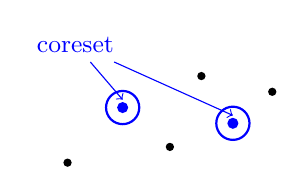
\begin{tikzpicture}
  			% all data points
  			\foreach \x/\y in {0.5/0.7, 1.2/1.4, 1.8/0.9, 2.2/1.8, 2.6/1.2, 3.1/1.6}
    			{\fill (\x,\y) circle (1.5pt);}
  			% coreset points (highlighted)
  			\foreach \x/\y in {1.2/1.4, 2.6/1.2}{
    			\fill[blue] (\x,\y) circle (2pt);
    			\draw[blue, thick] (\x,\y) circle (6pt);
  			}
  			% a simple label pointing to both coreset elements
  			\node[blue] (label) at (0.6,2.2) {\small coreset};
  			\draw[->,blue] (label) -- (1.2,1.5);
  			\draw[->,blue] (label) -- (2.6,1.3);
			\end{tikzpicture}
		\caption{A coreset (highlighted in blue) is a small subset of a larger \gls{dataset}. \label{fig_coreset_dict}}
		\end{figure}
		Coresets are particularly useful for \gls{ml} applications (such as \gls{clustering}) 
		involving large \glspl{dataset}, as they allow for efficient computation while 
		preserving the essential characteristics of the \gls{data} \cite{DistkmeansBalcan2013}.
				\\
		See also: \gls{dataset}, \gls{datapoint}, \gls{clustering}.},
	first={coreset},
	firstplural={coresets},
	plural={coresets},
	text={coreset} 
}

\newglossaryentry{outlier}
{name={outlier}, 
	description={Many\index{outlier} \gls{ml} methods 
		are motivated by the \gls{iidasspt}, which interprets \glspl{datapoint} as \glspl{realization} of 
		\gls{iid} \glspl{rv} with a common \gls{probdist}. The \gls{iidasspt} is useful for applications  
		where the statistical properties of the \gls{data} generation process are stationary (or time-invariant) \cite{Brockwell91}. 
		However, in some applications, the \gls{data} consist of a majority of regular \glspl{datapoint} 
		that conform with the \gls{iidasspt} as well as a small number of \glspl{datapoint} that have fundamentally different 
       		statistical properties compared with the regular \glspl{datapoint}. We refer to 
		a \gls{datapoint} that substantially deviates from the statistical properties of 
		most \glspl{datapoint} as an outlier. Different methods for outlier detection 
		use different \glspl{measure} of this deviation. 
        		Statistical learning theory studies fundamental limits on the ability to 
		mitigate outliers reliably \cite{doi:10.1137/0222052}, \cite{10.1214/20-AOS1961}.
        		\\
		See also: \gls{robustness}, \gls{stability}, \gls{huberreg}, \gls{probmodel}.},
	 first={outlier},
	 text={outlier} 
}

\newglossaryentry{membershipinferenceattack}
{name={membership inference attack}, 
	description={Consider an \gls{ml} method that learns a \gls{hypothesis} 
		via \gls{erm} on a \gls{trainset}. Membership \gls{inference}\index{membership inference attack} 
                \gls{attack} is a form of \gls{privattack} where an adversary tries 
		to determine whether a particular \gls{datapoint} was part 
		of the \gls{trainset}. The attacker typically queries 
		$\learnthypothesis$ with candidate \glspl{featurevec} 
		$\featurevec^{(1)},\,\ldots,\,\featurevec^{(\nrbootstraps)}$, 
		and infers the membership status of a given \gls{datapoint} 
		based on the \glspl{prediction} $\learnthypothesis\big(\featurevec^{(1)}\big),\,\ldots,
		\,\learnthypothesis\big(\featurevec^{(\nrbootstraps)}\big)$ \cite{Shokri2017}.
		\\ 
		See also: \gls{attack}, \gls{privattack}.}, 
 	first={membership inference attack}, 
 	text={membership inference attack}
}

\newglossaryentry{machineunlearning}
{name={machine unlearning},
	description={Consider an \gls{ml} method that learns a \gls{hypothesis} $\learnthypothesis$ 
		via \gls{erm} on a \gls{trainset} $\dataset$. The learned \gls{hypothesis} can 
		reveal information about $\dataset$, which is exploited by \glspl{privattack} such as 
		\gls{modelinversion}. Machine unlearning\index{machine unlearning} refers to techniques that 
		modify $\learnthypothesis$, so that it is harder to infer properties of individual 
		\glspl{datapoint} in $\dataset$ \cite{cao2015unlearning}. Machine unlearning helps 
		to meet legal requirements for \gls{privprot} in \glspl{aisystem} \cite{GDPR2016}. 
		\\
	 	See also: \gls{modelinversion}, \gls{privprot}, \gls{gdpr}. },
	first={machine unlearning},
	text={machine unlearning}
}

% Shouldn't this be ensemble method?
\newglossaryentry{ensemble}
{name={ensemble}, 
	description={An ensemble method\index{ensemble} combines multiple 
		\gls{ml} methods, each of those referred to as a \gls{baselearner}, 
		to improve overall performance. The \glspl{baselearner} can be \gls{erm}-based 
        		using different choices for the \gls{loss}, \gls{model}, and \gls{trainset}. 
		By aggregating the \glspl{prediction} of \glspl{baselearner}, ensemble methods can 
		often achieve better performance than any single \gls{baselearner}. The 
		aggregation can amount to averaging the \glspl{prediction} of \glspl{baselearner} 
		(in \gls{regression}) or using a majority vote (for \gls{classification} methods). 
		\begin{figure}[H]
		\begin{center}
			\begin{tikzpicture}[
				scale=1.1, transform shape,
				node distance=11mm and 10mm,
				dataset/.style={draw, rounded corners, inner sep=2pt},
				learner/.style={draw, rounded corners,inner sep=2pt},
				op/.style={draw, circle, inner sep=1pt},
				flow/.style={->, >=latex},
				feedback/.style={->, >=latex, dashed, very thin},
				lab/.style={font=\scriptsize}
				]
				% --- Source dataset
				\node[dataset] (D) {$\dataset$};
				% --- Variant datasets (could be resample/reweight/transform)
				\node[dataset, below left=of D]  (D1) {\small $\widetilde{\dataset}^{(1)}$};
				\node[dataset, below=of D]       (D2) {\small $\widetilde{\dataset}^{(2)}$};
				\node[dataset, below right=of D] (D3) {\small $\widetilde{\dataset}^{(3)}$};
				\draw[flow] (D) -- (D1) node[midway, lab, above left=-1pt] {resample};
				\draw[flow] (D) -- (D2) node[midway, lab, right] {};
				\draw[flow] (D) -- (D3) node[midway, lab, above right=-1pt] {};
				% --- Base learners
				\node[learner, below=5mm of D1] (L1) {\small $\hypospace^{(1)}$};
				\node[learner, below=5mm of D2] (L2) {\small $\hypospace^{(2)}$};
				\node[learner, below=5mm of D3] (L3) {\small $\hypospace^{(3)}$};
				% --- Data-to-learner edges
				\draw[flow] (D1) -- (L1);
				\draw[flow] (D2) -- (L2);
				\draw[flow] (D3) -- (L3);
				% --- Inter-learner dependencies (generic; like boosting-style feedback)
				\draw[feedback] (L1.east) .. controls +(+7mm,0mm) and +(-7mm,0mm) .. (L2.west)
				node[midway, lab, above] {};
				\draw[feedback] (L2.east) .. controls +(+7mm,0mm) and +(-7mm,0mm) .. (L3.west);
				% (Optional: allow skip connections)
				\draw[feedback] (L1.east) to[out=60, in=120] (L3.west);
				% --- Aggregator and final prediction
				\node[op, below=8mm of L2] (agg) {\small $\phi_{\text{agg}}$};
				\draw[flow] (L1) -- (agg);
				\draw[flow] (L2) -- (agg);
				\draw[flow] (L3) -- (agg);
				% --- Prediction display
				\node[below=5mm of agg, align=right, inner sep=2pt] (yhat)
				{\small $\learnthypothesis= \phi_{\text{agg}}\!\big(\learntlocalhypothesis{1},\,\learntlocalhypothesis{2},\,\learntlocalhypothesis{3}\big)$};
				\draw[flow] (agg) -- (yhat);
				% --- Tiny labels on learner outputs
				\node[lab, below left=-1pt and -1pt of L1.south] {$\learntlocalhypothesis{1}$};
				\node[lab, below           =-1pt of L2.south]    {$\learntlocalhypothesis{2}$};
				\node[lab, below right=-1pt and -1pt of L3.south]{$\learntlocalhypothesis{3}$};
				% --- Mini legend for dashed feedback
				%	\node[lab, above right=2mm and 0mm of L3] (leg) {dashed: inter-learner info};
				%	\draw[feedback] ($(leg.west)+(0mm,-1.5mm)$) -- ++(-8mm,0mm);
			\end{tikzpicture}
			\caption{A generic ensemble with three \glspl{baselearner}, each  
				using \gls{erm} to learn $\hypospace^{(\featureidx)} \in \hypospace^{(\featureidx)}$ 
				based on the \gls{trainset} $\widetilde{\dataset}^{(\featureidx)}$. A \gls{baselearner} might also 
				use the \gls{output} of other \glspl{baselearner}. The final \gls{hypothesis} $\learnthypothesis$ 
				is obtained by aggregating the \glspl{hypothesis} generated by the \glspl{baselearner}.}
		\end{center}
		\end{figure}
		Different ensemble methods use different constructions for the \glspl{baselearner}. 
		For example, \gls{bagging} methods (such as a \gls{randomforest}) use random sampling to 
		construct slightly different \glspl{trainset} for each \gls{baselearner}. 
	    	On the other hand, \gls{boosting} methods run the \glspl{baselearner} 
		sequentially, i.e., each \gls{baselearner} tries to correct the \gls{prediction} 
		errors of the previous ones. A third family of ensemble methods is \gls{stacking}, 
		where \glspl{baselearner} are trained on the same \gls{trainset} but with 
		different \glspl{model}.
		\\
	 	See also: \gls{bagging}, \gls{boosting}, \gls{stacking}.},
	 first={ensemble},
	 text={ensemble} 
}

\newglossaryentry{stacking}
{name={stacking}, 
	description={Stacking\index{stacking} is one of the main types of \gls{ensemble} methods.  
		In stacking, a finite number $\numlearners$ of \glspl{baselearner} are trained on the 
		same \gls{dataset} but with different \glspl{model} $\hypospace^{(\featureidx)}$ 
		or \glspl{lossfunc} $\loss^{(\featureidx)}$ for $\featureidx=1,\,\ldots,\,\numlearners$ \cite[Ch. 8.8]{hastie01statisticallearning},
		\cite{WOLPERT1992241}, \cite{ZhouEnsemble2012}. 
		The $\featureidx$th \gls{baselearner} delivers a learned \gls{hypothesis} 
		$\learntlocalhypothesis{\featureidx} \in \hypospace^{(\featureidx)}$. 
		The final \gls{prediction} for a \gls{datapoint} is obtained by aggregating the 
		\glspl{prediction} of the \glspl{baselearner} via an aggregation rule $\phi_{\rm agg}$, 
		such as majority voting for \gls{classification} or averaging for \gls{regression}. 
		We can interpret stacking as a form of \gls{featlearn}, where each \gls{baselearner} 
		extracts a new \gls{feature}. The aggregation rule can be obtained by another instance 
		of \gls{erm} that learns a \gls{hypothesis} \gls{map} $\phi_{\rm agg} \in \hypospace$ from 
		a meta-\gls{model} $\hypospace$. The \gls{hypothesis} $\phi_{\rm agg}$ is applied to the 
		transformed \gls{featurevec} $$\featuremapvec(\featurevec)= \big( \learnthypothesis^{(1)}(\featurevec), 
       		\,\ldots, \,\learnthypothesis^{(\numlearners)}(\featurevec) \big)^{T}.$$
       		\begin{figure}[H]
			\begin{center}
			\begin{tikzpicture}[
			font=\small,
			scale=1.0, transform shape,
			node distance=7mm and 10mm,
			dataset/.style={draw, rounded corners, inner sep=2pt},
			learner/.style={draw, rounded corners, minimum width=14mm, minimum height=7mm, inner sep=6pt,align=center},
			op/.style={draw, circle, inner sep=1pt},
			>=latex
			]
			% Original dataset
			\node[dataset] (D) {$\dataset$};
			% Variants (closer to D)
			\node[learner, below left=of D]  (L1) {\gls{erm} \\ $\hypospace^{(1)},\loss^{(1)}$};
			\node[learner, below=of D]       (L2) {\gls{erm} \\ $\hypospace^{(2)},\loss^{(2)}$};
			\node[learner, below right=of D] (L3) {\gls{erm} \\ $\hypospace^{(3)},\loss^{(3)}$};
			% Arrows to variants (shorter labels)
			\draw[->] (D) -- (L1) node[midway, above left=-1pt] {};
			\draw[->] (D) -- (L2) node[midway, right]           {};
			\draw[->] (D) -- (L3) node[midway, above right=-1pt]{};
			\node[op, below=8mm of L2] (agg) {$\phi_{\text{agg}}$};
			\node[below=5mm of agg, align=right, inner sep=2pt] (yhat)
			{$\predictedlabel = \phi_{\text{agg}}\!\big(\learntlocalhypothesis{1}(\featurevec),\learntlocalhypothesis{2}(\featurevec),\learntlocalhypothesis{3}(\featurevec)\big)$};
			\draw[->] (L1) -- (agg);
			\draw[->] (L2) -- (agg);
			\draw[->] (L3) -- (agg);
			\draw[->] (agg) -- (yhat);
			% Tiny labels on learner outputs
			\node[below left=-1pt and -1pt of L1.south] {$\learntlocalhypothesis{1}$};
			\node[below           =-1pt of L2.south]    {$\learntlocalhypothesis{2}$};
			\node[below right=-1pt and -1pt of L3.south]{$\learntlocalhypothesis{3}$};
			\end{tikzpicture}
		\caption{Three \glspl{baselearner} using \gls{erm} with 
			different \glspl{model} and \glspl{lossfunc} to obtain learned \glspl{hypothesis} 
			$\learntlocalhypothesis{1},\,\learntlocalhypothesis{2},\,\learntlocalhypothesis{3}$. 
			For a \gls{datapoint} with \gls{featurevec} $\featurevec$, each \gls{baselearner} delivers a \gls{prediction}  
			$\learntlocalhypothesis{\featureidx}(\featurevec)$ for $\featureidx=1,\,2,\,3$. These 
			\glspl{prediction} are then used as new \glspl{feature} for an aggregation 
			rule $\phi_{\rm agg}$ that delivers the overall \gls{prediction} $\predictedlabel$. 
			The aggregation rule can be obtained by \gls{training} a meta-\gls{model} $\hypospace$.}
			\end{center}
		\end{figure}
	 	See also: \gls{ensemble}, \gls{bagging}.},
	 first={stacking},
	 text={stacking} 
}

\newglossaryentry{auc}
{name={area under the curve (AUC)}, 
	description={The AUC\index{area under the curve (AUC)} is a quantitative \gls{measure} of the 
 		usefulness of a binary \gls{classifier} \cite{Hanley:1982aa}. It 
		is defined (using the natural \gls{measure} of the \gls{euclidspace} $\mathbb{R}^{2}$) as the area  
		under the \gls{roc} curve.
		\\
		See also: \gls{classifier}, \gls{euclidspace}, \gls{roc}. } , 
 	first={area under the curve (AUC)}, 
 	text={AUC} 
}

\newglossaryentry{roc} 
{name={receiver operating characteristic (ROC)}, 
	description={Consider a \gls{labelspace} $\labelspace=\{-1,1\}$ and a \gls{classifier} 
 		that uses a real-valued \gls{hypothesis} $\hypothesis(\featurevec)$. For a given 
 		threshold $\eta \in \mathbb{R}$, the ultimate \gls{prediction} is $\predictedlabel=1$ 
 		if $\hypothesis(\featurevec)\geq \eta$ and $\predictedlabel=-1$ otherwise. 
 		On a \gls{testset} $\testset$, we compute, for each value of $\eta$, 
		the following two quantities: 1) true positive rate ${\rm TPR}^{(\eta)}$; 
		and 2) false positive rate ${\rm FPR}^{(\eta)}$. 
 		The ROC curve\index{receiver operating characteristic (ROC)} is  
 		the following \gls{function} \cite{IntroROCFawcett}:
 		$${\rm ROC}: \mathbb{R} \rightarrow \mathbb{R}^{2}: \eta \mapsto \big({\rm TPR}^{(\eta)}, {\rm FPR}^{(\eta)} \big).$$ 
 	        One important characteristic of the ROC curve is the \gls{auc}.
	        \\ 
 		See also: \gls{classifier}, \gls{auc}.}, 
  	first={receiver operating characteristic (ROC)}, 
  	text={ROC}
}

\newglossaryentry{bagging}
{name={bagging},
	description={Bagging\index{bagging} is an \gls{ensemble} technique where \glspl{baselearner} 
		use perturbed copies $$\widetilde{\dataset}^{(1)},\,\ldots,\,\widetilde{\dataset}^{(\numlearners)}$$ 
		of the original \gls{trainset} $\dataset$ \cite{Breiman:1996aa}. Each 
		\gls{baselearner} delivers a potentially different \gls{hypothesis} $$\learnthypothesis^{(1)},\,\ldots,\,\learnthypothesis^{(\numlearners)}.$$
		The \gls{hypothesis} delivered by the overall method is obtained by 
		aggregating the \glspl{hypothesis} $\learnthypothesis^{(1)},\,\ldots,\,\learnthypothesis^{(\numlearners)}$ 
		using some aggregation rule. For \gls{classification} methods, the rule is typically 
		a majority vote, while for \gls{regression} methods, it amounts to averaging. 
		\begin{figure}[H]
			\begin{center}
			\begin{tikzpicture}[
			scale=1.0, transform shape,
			node distance=10mm and 10mm,
			dataset/.style={draw, rounded corners, inner sep=2pt},
			learner/.style={draw, rounded corners, minimum width=14mm, minimum height=7mm, inner sep=2pt},
			op/.style={draw, circle, inner sep=1pt},
			>=latex
			]
			% Original dataset
			\node[dataset] (D) {$\dataset$};
			% Variants (closer to D)
			\node[dataset, below left=of D]  (D1) {$\widetilde{\dataset}^{(1)}$};
			\node[dataset, below=of D]       (D2) {$\widetilde{\dataset}^{(2)}$};
			\node[dataset, below right=of D] (D3) {$\widetilde{\dataset}^{(3)}$};
			% Arrows to variants (shorter labels)
			\draw[->] (D) -- (D1) node[midway, above left=-1pt] {resample};
			\draw[->] (D) -- (D2) node[midway, right]           {resample};
			\draw[->] (D) -- (D3) node[midway, above right=-1pt]{resample};
			% Base learners (reduced vertical gaps)
			\node[learner, below=5mm of D1] (L1) {$\hypospace^{(1)}$};
			\node[learner, below=5mm of D2] (L2) {$\hypospace^{(2)}$};
			\node[learner, below=5mm of D3] (L3) {$\hypospace^{(3)}$};
			% Feed variants into learners
			\draw[->] (D1) -- (L1);
			\draw[->] (D2) -- (L2);
			\draw[->] (D3) -- (L3);
			% Aggregator and final prediction (tighter)
			\node[op, below=8mm of L2] (agg) {$\phi_{\text{agg}}$};
			\node[below=5mm of agg, align=right, inner sep=2pt] (yhat)
			{$\learnthypothesis = \phi_{\text{agg}}\!\big(\learntlocalhypothesis{1},\learntlocalhypothesis{2},\learntlocalhypothesis{3}\big)$};
			\draw[->] (L1) -- (agg);
			\draw[->] (L2) -- (agg);
			\draw[->] (L3) -- (agg);
			\draw[->] (agg) -- (yhat);
			% Tiny labels on learner outputs
			\node[below left=-1pt and -1pt of L1.south] {$\learntlocalhypothesis{1}$};
			\node[below           =-1pt of L2.south]    {$\learntlocalhypothesis{2}$};
			\node[below right=-1pt and -1pt of L3.south]{$\learntlocalhypothesis{3}$};
			\end{tikzpicture}
		\caption{An example of bagging where three \glspl{baselearner} use perturbations  
			$\widetilde{\dataset}^{(1)},\,\ldots,\,\widetilde{\dataset}^{(3)}$ of 
			the original \gls{trainset} $\dataset$ to learn the \glspl{hypothesis} 
			$\learntlocalhypothesis{1},\,\ldots,\,\learntlocalhypothesis{3}$. The final 
			\gls{hypothesis} is obtained by aggregating these individual \glspl{hypothesis} 
			via some aggregation rule $\phi_{\rm agg}$.}
			\end{center}
		\end{figure}
		See also: \gls{ensemble}, \gls{robustness}, \gls{bootstrap}.},
	first={bagging},
	text={bagging}
}

\newglossaryentry{bootstrap aggregation}
{name={bootstrap aggregation}, 
	description={See \gls{bagging}\index{bootstrap aggregation}.},
 	first={bootstrap aggregation},
 	text={bootstrap aggregation} 
}	

\newglossaryentry{decisionregion}
{name={decision region},
	description={Consider\index{decision region} 
		a \gls{hypothesis} \gls{map} $\hypothesis$ that delivers values from a finite set $\labelspace$. 
		For each \gls{label} value (i.e., category) $a \in \labelspace$, the \gls{hypothesis} $\hypothesis$ 
		determines a subset of \gls{feature} values $\featurevec \in \featurespace$ that result 
		in the same \gls{output} $\hypothesis(\featurevec)=a$. We refer to this subset as a decision 
		region of the \gls{hypothesis} $\hypothesis$. 
		\\
		See also: \gls{hypothesis}, \gls{map}, \gls{label}, \gls{feature}.},
	first={decision region},
	plural={decision regions}, 
	firstplural={decision regions}, 
	text={decision region} 
}

\newglossaryentry{baselearner}
{name={base learner}, 
	description={A base learner\index{base learner} is an \gls{ml} method 
         	that is part of an \gls{ensemble} method. 
		\\
		See also: \gls{ensemble}, \gls{bagging}, \gls{stacking}, \gls{boosting}.},
	first={base learner},
	firstplural={base learners},
	plural={base learners},
	text={base learner} 
}	

\newglossaryentry{decisionboundary}
{name={decision boundary}, 
	description={Consider\index{decision boundary} a 
		\gls{hypothesis} \gls{map} $\hypothesis$ that reads in a \gls{featurevec}  
		$\featurevec \in \mathbb{R}^{\featuredim}$ and delivers a value from a finite set $\labelspace$. 
		The decision \gls{boundary} of $\hypothesis$ is the set of \glspl{vector} $\featurevec \in \mathbb{R}^{\featuredim}$ 
		that lie between different \glspl{decisionregion}. More precisely, a 
		\gls{vector} $\featurevec$ belongs to the decision \gls{boundary} if and only 
		if each \gls{neighborhood} $\{ \featurevec': \| \featurevec - \featurevec' \| \leq \varepsilon \}$, 
		for any $\varepsilon >0$, contains at least two \glspl{vector} with different \gls{function} values.
				\\
		See also: \gls{hypothesis}, \gls{map}, \gls{featurevec}, \gls{boundary}, \gls{vector}, \gls{decisionregion}, 
		\gls{neighborhood}, \gls{function}.},
	first={decision boundary},
	firstplural={decision boundaries},
	plural={decision boundaries},
	text={decision boundary} 
}

\newglossaryentry{normalequations}
{name={normal equations}, 
	description={Consider \gls{linleastsquares}\index{normal equations}, which learns the \glspl{parameter} of a 
		\gls{linmodel} by minimizing the average \gls{sqerrloss} on a 
		\gls{trainset} $\dataset$. 
		The learned \glspl{parameter} $\widehat{\weights}$ are characterized by the 
		linear system of equations, i.e.,
		\begin{equation} 
			\label{equ_normal_equations_dict}
			\featuremtx^{T} \featuremtx \widehat{\weights} = \featuremtx^{T} \labelvec.
		\end{equation} 
		Here, $\featuremtx=\big(\featurevec^{(1)},\,\ldots,\,\featurevec^{(\samplesize)}\big)^{T} \in \mathbb{R}^{\samplesize \times \nrfeatures}$ 
		is the \gls{featuremtx} of $\dataset$ and $\labelvec=\big(\truelabel^{(1)},\,\ldots,\,\truelabel^{(\samplesize)} \big)^{T} \in \mathbb{R}^{\samplesize}$ 
		is the \gls{labelvec} of $\dataset$. This linear system of equations is referred 
		to as normal equations, as it amounts to an orthogonality condition. Indeed, \eqref{equ_normal_equations_dict} 
		can be rewritten as $$ \featuremtx^{T} \big( \featuremtx \widehat{\weights} - \labelvec \big) = \mathbf{0}.$$
		This means that the \gls{prediction} error \gls{vector} $\featuremtx \widehat{\weights} - \labelvec$ 
		is orthogonal to the columns of $\featuremtx$ and, in turn, to the \gls{subspace} $\linspan{\featuremtx}$
		spanned by them.
		\\ 
		See also: \gls{linleastsquares}, \gls{modelparam}. },
	first={normal equations},
	text={normal equations} 
}

\newglossaryentry{eerm}
{name={explainable empirical risk minimization (EERM)}, 
	description={EERM is an\index{explainable empirical risk minimization (EERM)} 
		in-\linebreak stance of \gls{srm} that adds a \gls{regularization} term to the 
		average \gls{loss} in the \gls{objfunc} of \gls{erm}. 
		The \gls{regularization} term is chosen to favor \gls{hypothesis} \glspl{map} that are intrinsically 
		explainable for a specific user. This user is characterized by their \glspl{prediction} provided 
		for the \glspl{datapoint} in a \gls{trainset} \cite{Zhang:2024aa}.
				\\
		See also: \gls{srm}, \gls{regularization}, \gls{erm}, \gls{trainset}.},
	first={explainable empirical risk minimization (EERM)},
	text={EERM} 
}
	
\newglossaryentry{kmeans}
{name={$k$-means}, 
sort={k-means},
	description={The\index{$k$-means} $k$-\glspl{mean} principle is an \gls{optimization}-based 
	    	approach to the \gls{clustering} of \glspl{datapoint} with a numeric \gls{featurevec} \cite[Ch. 8]{MLBasics}. 
		As a \gls{hardclustering} approach, $k$-\glspl{mean} partitions a \gls{dataset} into $k$ disjoint 
		subsets (or \glspl{cluster}), which are indexed by $\clusteridx=1,\,\ldots,\,\nrcluster$. Each \gls{cluster} $\cluster$ 
		is characterized by the average \gls{featurevec} of \glspl{datapoint} that belong to it. This average 
		(or \gls{mean}) \gls{featurevec} is referred to as the \gls{clustercentroid} $\clustercentroid{\clusteridx}$. 
		A visual illustration is provided in Fig. \ref{fig_kmeans_dict}.
		\begin{figure}[H]
		\begin{center}
		\begin{tikzpicture}[scale=1]
			% Styles
			\tikzset{
			data/.style={circle, fill=black, inner sep=1.2pt},
			centroid/.style={thick, cross out, draw, minimum size=6pt, inner sep=0pt}
			}
			% Cluster A data (with one labeled point)
			\node[data] (xi) at (1.0,0.2) {};
			\node[right=0pt of xi,yshift=2pt] {$\featurevec^{(\sampleidx)}$};
			% The rest unlabeled
			\foreach \p in {(-0.3,0.0),(0.2,-0.4),(0.6,0.8),(0.0,0.9),(1.1,-0.2)}
			\node[data] at \p {};
			% Cluster B data (spread wider)
			\foreach \p in {(2.5,1.0),(3.7,1.2),(2.6,2.3),(3.8,2.5),(3.0,2.9),(3.6,1.6)}
			\node[data] at \p {};
			% Centroids as crosses
			\node[centroid] (mu1) at (0.55,0.4) {};
			\node[centroid] (mu2) at (3.1,1.85) {};
			% Labels
			\node[above of=mu1,yshift=-25pt,xshift=-10pt] {$\clustercentroid{1}$};
			\node[above of=mu2,yshift=-25pt,xshift=-10pt] {$\clustercentroid{2}$};
		\end{tikzpicture}
		\end{center}
		\caption{A \gls{scatterplot} of \glspl{datapoint}, indexed by $\sampleidx=1,\,\ldots,\,\samplesize$ and 
			characterized by \glspl{featurevec} $\featurevec^{(\sampleidx)} \in \mathbb{R}^{2}$. 
			The \gls{scatterplot} also includes two \glspl{clustercentroid} $\clustercentroid{1}, \clustercentroid{2} \in \mathbb{R}^{2}$. \label{fig_kmeans_dict}}
		\end{figure} 
		In general, solving the $k$-\glspl{mean} \gls{optproblem} exactly is challenging (or NP-hard) 
		\cite{Mahajan2009Springer}. However, there are simple iterative methods for finding 
		approximately optimal \glspl{clustercentroid}. One such method is referred to as 
		\gls{lloydalgorithm}.
		\\
		See also: \gls{hardclustering}, \gls{cluster}, \gls{lloydalgorithm}.},
	first={$k$-means},
	text={$k$-means} 
}

\newglossaryentry{lloydalgorithm} 
{name={Lloyd's algorithm}, 
	description={Lloyd's\index{Lloyd's algorithm} \gls{algorithm} \cite{Lloyd1982} is an iterative 
		\gls{optmethod} for finding \glspl{clustercentroid} that are approximately 
	   	optimal for the \gls{kmeans} \gls{objfunc}. Lloyd's \gls{algorithm}  
	   	alternates between: 1) updating the \gls{cluster} assignment of each \gls{datapoint} 
		based on the nearest current \gls{clustercentroid}; and 
		2) recalculating the \glspl{clustercentroid} given the updated 
		\gls{cluster} assignments \cite{Lloyd1982}.
		\begin{figure}[H]
			\begin{center}
			\begin{tikzpicture}[
			assignment/.style={-Latex, very thin},
			move/.style={-Latex, thick},
			center/.style={draw, circle, inner sep=1.2pt, fill=white},
			pointA/.style={circle, inner sep=1.1pt, fill=black},
			pointB/.style={rectangle, inner sep=1.1pt, fill=black},
			cross/.style={line width=0.4pt},
			lab/.style={font=\scriptsize}
			]
			% ===================== PANEL (a): Initial centers =====================
			% ===================== PANEL (b): Assign to nearest =====================
			\begin{scope}[shift={(0,0)}]
				% points
				\coordinate (Ba1) at (0.2, 1.1);
				\coordinate (Ba2) at (0.4, 0.6);
				\coordinate (Ba3) at (0.8, 1.0);
				\coordinate (Ba4) at (0.6, 0.2);
				\coordinate (Bb1) at (2.7, 1.4);
				\coordinate (Bb2) at (3.2, 0.9);
				\coordinate (Bb3) at (2.6, 0.3);
				\coordinate (Bb4) at (3.3, 0.2);
				\node[pointA] at (Ba1) {}; \node[pointA] at (Ba2) {}; \node[pointA] at (Ba3) {}; \node[pointA] at (Ba4) {};
				\node[pointB] at (Bb1) {}; \node[pointB] at (Bb2) {}; \node[pointB] at (Bb3) {}; \node[pointB] at (Bb4) {};
				% centers (old)
				\coordinate (Bc1old) at (0.9,0.65);
				\coordinate (Bc2old) at (2.8,1.8);
				\node[center,label={[lab, xshift=-2pt]right:$\clustercentroiditer{1}{\iteridx}$}] (B-C1) at (Bc1old) {};
				\node[center,label={[lab, xshift=-2pt]right:$\clustercentroiditer{2}{\iteridx}$}] (B-C2) at (Bc2old) {};
				% perpendicular bisector
				\path let 
				\p1=(B-C1), \p2=(B-C2),
				\n1={(\x2-\x1)}, \n2={(\y2-\y1)},
				\n3={veclen(\n1,\n2)}
				in coordinate (B-M)    at ($ (B-C1)!0.5!(B-C2) $)
				coordinate (B-Nhat) at ($ (0,0) + ({-\n2/\n3},{\n1/\n3}) $);
				\draw[dashed, thick] ($ (B-M) + 10.4*(B-Nhat) $) -- ($ (B-M) - 10.4*(B-Nhat) $);
				% minimal assignment spokes
				\draw[assignment] (Ba2) -- (B-C1);
				\draw[assignment] (Ba3) -- (B-C1);
				\draw[assignment] (Bb2) -- (B-C2);
				\draw[assignment] (Bb3) -- (B-C2);
				\node[lab] at (1.6,-0.35) {Assign to the nearest \gls{clustercentroid}.};
				\node at (1.6,-1.3) {(a)};
			\end{scope}
			% ===================== PANEL (c): Recompute means =====================
			\begin{scope}[shift={(5.5,0)}]
				% points
				\coordinate (Ca1) at (0.2, 1.1);
				\coordinate (Ca2) at (0.4, 0.6);
				\coordinate (Ca3) at (0.8, 1.0);
				\coordinate (Ca4) at (0.6, 0.2);
				\coordinate (Cb1) at (2.7, 1.4);
				\coordinate (Cb2) at (3.2, 0.9);
				\coordinate (Cb3) at (2.6, 0.3);
				\coordinate (Cb4) at (3.3, 0.2);
				\node[pointA] at (Ca1) {}; \node[pointA] at (Ca2) {}; \node[pointA] at (Ca3) {}; \node[pointA] at (Ca4) {};
				\node[pointB] at (Cb1) {}; \node[pointB] at (Cb2) {}; \node[pointB] at (Cb3) {}; \node[pointB] at (Cb4) {};
				% centers (old and new)
				\coordinate (Cc1old) at (0.9,0.65);
				\coordinate (Cc2old) at (2.8,1.8);
				\coordinate (Cc1new) at (0.5,0.725);
				\coordinate (Cc2new) at (2.95,0.70);
				\node[center, opacity=0.5] at (Cc1old) {};
				\node[center, opacity=0.5] at (Cc2old) {};
				% crosses for new centers
				\draw[cross] ($(Cc1new)+(-0.07,0)$) -- ($(Cc1new)+(0.07,0)$);
				\draw[cross] ($(Cc1new)+(0,-0.07)$) -- ($(Cc1new)+(0,0.07)$);
				\draw[cross] ($(Cc2new)+(-0.07,0)$) -- ($(Cc2new)+(0.07,0)$);
				\draw[cross] ($(Cc2new)+(0,-0.07)$) -- ($(Cc2new)+(0,0.07)$);
				% movement arrows
				\draw[move] (Cc1old) -- (Cc1new);
				\draw[move] (Cc2old) -- (Cc2new);
				\node[lab] at (1.6,-0.35) {Recompute \glspl{clustercentroid}.};
				\node at (1.6,-1.3) {(b)};
			\end{scope}
			% ===================== PANEL (d): Update & new partition =====================
			\begin{scope}[shift={(3,-4)}]
				% points
				\coordinate (Da1) at (0.2, 1.1);
				\coordinate (Da2) at (0.4, 0.6);
				\coordinate (Da3) at (0.8, 1.0);
				\coordinate (Da4) at (0.6, 0.2);
				\coordinate (Db1) at (2.7, 1.4);
				\coordinate (Db2) at (3.2, 0.9);
				\coordinate (Db3) at (2.6, 0.3);
				\coordinate (Db4) at (3.3, 0.2);
				\node[pointA] at (Da1) {}; \node[pointA] at (Da2) {}; \node[pointA] at (Da3) {}; \node[pointA] at (Da4) {};
				\node[pointB] at (Db1) {}; \node[pointB] at (Db2) {}; \node[pointB] at (Db3) {}; \node[pointB] at (Db4) {};
				% centers (new)
				\coordinate (Dc1new) at (0.5,0.725);
				\coordinate (Dc2new) at (2.95,0.70);
				\node[center, label={[lab, xshift=-2pt]right:$\clustercentroiditer{1}{\iteridx+1}$}] (D-C1n) at (Dc1new) {};
				\node[center, label={[lab]right:$\clustercentroiditer{2}{\iteridx+1}$}] (D-C2n) at (Dc2new) {};
				% perpendicular bisector
				\path let 
				\p1=(D-C1n), \p2=(D-C2n),
				\n1={(\x2-\x1)}, \n2={(\y2-\y1)},
				\n3={veclen(\n1,\n2)}
				in coordinate (D-M)    at ($ (D-C1n)!0.5!(D-C2n) $)
				coordinate (D-Nhat) at ($ (0,0) + ({-\n2/\n3},{\n1/\n3}) $);
				\draw[dashed, thick] ($ (D-M) + 10.4*(D-Nhat) $) -- ($ (D-M) - 10.4*(D-Nhat) $);
				\node[lab] at (1.6,-0.35) {Assign to the nearest \gls{clustercentroid}.};
				\node at (1.6,-1.3) {(c)};
			\end{scope}
			\end{tikzpicture}
			\end{center}
		\caption{Lloyd's \gls{algorithm} alternates between (a) and (c) assigning \glspl{datapoint} to 
			the nearest \gls{clustercentroid} and, in turn, (b) recomputing the \glspl{clustercentroid} 
			based on the new \gls{cluster} assignments. 
			\label{fig_lloyd_algorithm_dict}}
		\end{figure}
		See also: \gls{clustercentroid}, \gls{kmeans}, \gls{clustering}.},
	first={Lloyd's algorithm},
	text={Lloyd's algorithm} 
}

\newglossaryentry{qlearning} 
{name={Q-learning}, 
	description={Q-learning\index{Q-learning} is a popular \gls{reinforcementlearning} 
	     	\gls{algorithm} that learns an optimal \gls{policy} by estimating the optimal \gls{action}-value 
		\gls{function} (or Q-\gls{function}) \cite{SuttonEd2}.  
		\\
		See also: \gls{reinforcementlearning}, \gls{fixedpointiter}.},
	first={Q-learning},
	text={Q-learning} 
}

\newglossaryentry{iteration}
{name={iteration},
	description={The elementary computational step during the execution of an 
		\gls{algorithm} is referred to as iteration\index{iteration} 
		\cite{Cormen:2022aa}, \cite{KleinbergTardos2006}. 
		For example, the elementary computational step of \glspl{gdmethod} 
		is a \gls{gradstep}. 
		More generally, the elementary computational step of a \gls{fixedpointiter} 
		is the evaluation of an underlying \gls{operator} $\fixedpointop$, which might 
		vary across iterations (see Fig. \ref{fig_iteration_dict}). 
		Many important \gls{ml} \glspl{algorithm}, including 
		\gls{lloydalgorithm} and \gls{gd}, are \glspl{fixedpointiter}.  
		\begin{figure}[H]
			\centering
			\begin{tikzpicture}[>=Latex, font=\small,scale=1]
			% --- baseline axis (purely visual) ---
			%			\draw[very thin] (-0.2,0) -- (5.6,0);
			% --- fixed point ---
			\node[circle,draw,inner sep=1.2pt,fill=white,label={above:$\weights^\ast$}] (xstar) at (8,0) {};
			% --- iterates ---
			\node[circle,fill,inner sep=1pt,label={below:$\weights^{(0)}$}] (x0) at (0.3,0) {};
			\node[circle,fill,inner sep=1pt,label={below:$\weights^{(1)}$}] (x1) at (4.3,0) {};
			\node[circle,fill,inner sep=1pt,label={below:$\weights^{(2)}$}] (x2) at (6.5,0) {};
			% --- update arrows labelled by the update operator T ---
			\draw[->] (x0) to[bend left=12] node[above,sloped] {$\fixedpointop$} (x1);
			\draw[->] (x1) to[bend left=12] node[above,sloped] {$\fixedpointop$} (x2);
			%\draw[->] (x5) to[bend left=12] node[above,sloped] {$\fixedpointop$} (xstar);
			% --- optional tiny stopping rule (comment out if too much) ---
			% \node[below=4pt of x4] {$\|x^{(t+1)} - x^{(t)}\| < \varepsilon$};
			\end{tikzpicture}
		\caption{A \gls{fixedpointiter} consists of the repeated application of an 
			\gls{operator} $\fixedpointop$ with some fixed point $\weights^\ast$, i.e., 
			$\fixedpointop\weights^\ast=\weights^\ast$. \label{fig_iteration_dict}}
		\end{figure} 
		See also: \gls{algorithm}, \gls{gradstep}, \gls{gd}.  },
	first={iteration},
	text={iteration},
	firstplural={iterations},
	plural={iterations}
}

\newglossaryentry{clustercentroid}
{name={cluster centroid}, 
	description={\Gls{clustering} methods\index{cluster centroid} decompose a given 
		\gls{dataset} into a few \glspl{cluster}. Different \gls{clustering} methods use 
		different representations for these \glspl{cluster}. If \glspl{datapoint} are 
		characterized by numerical \glspl{featurevec} $\featurevec \in \mathbb{R}^{\nrfeatures}$, 
		we can use some \gls{vector} ${\bm \mu} \in \mathbb{R}^{\nrfeatures}$, referred to 
		as \gls{cluster} centroid, to represent a \gls{cluster}. For example, if a \gls{cluster} 
		consists of a set of \glspl{datapoint}, we use the average of their \glspl{featurevec} 
		as a \gls{cluster} centroid. However, there are also other choices for how to construct 
		a \gls{cluster} centroid, e.g., using the \gls{geometricmedian} \cite{PARK20093336} 
		or via non-Euclidean geometry \cite{JMLR:v6:banerjee05b}.
		\\
		See also: \gls{clustering}, \gls{featurevec}, \gls{kmeans}.},
	first={cluster centroid},
	firstplural={cluster centroids}, 
	text={cluster centroid}, 
	plural={cluster centroids}
}

\newglossaryentry{xml}
{name={explainable machine learning (XML)}, 
	description={XML\index{explainable machine learning (XML)} 
		methods aim to complement each \gls{prediction} with an \gls{explanation} of 
		how the \gls{prediction} has been obtained. The construction of an explicit \gls{explanation} 
		might not be necessary if the \gls{ml} method uses a sufficiently simple (or interpretable) \gls{model} \cite{rudin2019stop}.
				\\
		See also: \gls{prediction}, \gls{explanation}, \gls{ml}, \gls{model}.},
	first={explainable machine learning (XML)},
	text={XML} 
}

\newglossaryentry{fmi}
{name={Finnish Meteorological Institute (FMI)}, 
	description={The\index{Finnish Meteorological Institute (FMI)}
		FMI is a government agency responsible for gathering 
		and reporting weather \gls{data} in Finland.
				\\
		See also: \gls{data}.},
	first={Finnish Meteorological Institute (FMI)},
	text={FMI} 
}
	
\newglossaryentry{samplemean}
{name={sample mean}, 
	description={The\index{sample mean} \gls{sample} \gls{mean} 
		$\vm \in \mathbb{R}^{\nrfeatures}$ for a given \gls{dataset}, with \glspl{featurevec} 
		$\featurevec^{(1)}, \,\ldots, \,\featurevec^{(\samplesize)} \in \mathbb{R}^{\nrfeatures}$, is defined as 
		$$\vm = \frac{1}{\samplesize} \sum_{\sampleidx=1}^{\samplesize} \featurevec^{(\sampleidx)}.$$ 
					\\
		See also: \gls{sample}, \gls{mean}, \gls{dataset}, \gls{featurevec}.},
	first={sample mean},
	text={sample mean} 
}
	
\newglossaryentry{highdimregime}
{name={high-dimensional regime}, 
	description={The\index{high-dimensional regime} 
		high-dimensional regime of \gls{erm} is characterized by the \gls{effdim} of the \gls{model} 
		being larger than the \gls{samplesize}, i.e., the number of (labeled) \glspl{datapoint} in the \gls{trainset}. 
		For example, \gls{linreg} methods operate in the high-dimensional regime whenever the number $\featuredim$ of \glspl{feature} 
		used to characterize \glspl{datapoint} exceeds the number of \glspl{datapoint} in the \gls{trainset}. 
		Another example of \gls{ml} methods that operate in the high-dimensional regime is large \glspl{ann}, which have 
		far more tunable \glspl{weight} (and bias terms) than the total number of \glspl{datapoint} in the \gls{trainset}. 
		High-dimensional statistics is a recent main thread of \gls{probability} theory that studies the 
		behavior of \gls{ml} methods in the high-dimensional regime \cite{Wain2019}, \cite{BuhlGeerBook}.
				\\
		See also: \gls{erm}, \gls{effdim}, \gls{overfitting}, \gls{regularization}.},
   	first={high-dimensional regime},
	text={high-dimensional regime} 
}

\newglossaryentry{gmm}
{name={Gaussian mixture model (GMM)}, 
	description={A GMM\index{Gaussian mixture model (GMM)} is a \gls{probmodel} 
		for (the generation of) \glspl{datapoint} with numeric \glspl{featurevec} 
		$\featurevec \in \mathbb{R}^\nrfeatures$ \cite{BishopBook}, \cite{Murphy2012}. 
		It assumes that each \gls{datapoint} is generated by first drawing 
		a latent \gls{cluster} index $I \in \{1,\,\ldots,\,\nrcluster\}$
		according to \gls{cluster} \glspl{probability} 
		$$\prob{I=\clusteridx} = p_{\clusteridx}, 
		\qquad 
		\sum_{\clusteridx=1}^{\nrcluster} p_{\clusteridx}=1.$$
		Conditioned on $I=\clusteridx$, the \gls{featurevec} $\featurevec$ 
		is drawn from a \gls{mvndist}
		$\probdist^{(\clusteridx)}= \mvnormal{\meanvec{\clusteridx}}{\covmtx{\clusteridx}}$.
		The resulting marginal distribution of $\featurevec$ is therefore 
		a weighted sum of \glspl{mvndist}, i.e.,
		$$\probdist
		=\sum_{\clusteridx=1}^{\nrcluster}
		p_{\clusteridx} \mvnormal{\meanvec{\clusteridx}}{\covmtx{\clusteridx}}.$$
		\begin{figure}[H]
		\begin{center}
		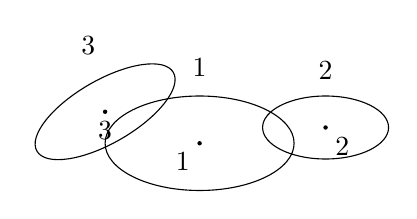
\begin{tikzpicture}[scale=0.4]
			% First component
			\draw (0,0) ellipse (3 and 1.5);
			\fill (0,0) circle (2pt);
			\node[below left] at (0,0) {$\meanvec{1}$};
			\node[above] at (0,1.8) {$\covmtx{1}$};
			% Second component
			\draw (4,0.5) ellipse (2 and 1);
			\fill (4,0.5) circle (2pt);
			\node[below right] at (4,0.5) {$\meanvec{2}$};
			\node[above] at (4,1.7) {$\covmtx{2}$};
			% Third (rotated) component
			\begin{scope}[rotate around={30:(-3,1)}]
			\draw (-3,1) ellipse (2.5 and 1);
			\end{scope}
			\fill (-3,1) circle (2pt);
			\node[below] at (-3,1) {$\meanvec{3}$};
			\node[above left] at (-3,2.5) {$\covmtx{3}$};
		\end{tikzpicture}
		\caption{Illustration of a GMM with three components. \label{fig_gmm_dict}}
		\end{center}
		\end{figure}
				%   \begin{figure}[H]
				%  	\begin{tikzpicture}[scale=0.4]
				%  		\draw [thick] \boundellipse{0,0}{10}{5} node[right]  {$\meanvec{1}$};
				%  		\fill (0,0) circle (2pt) ; 
				%  		\node [right] at (0,5.5) {$\covmtx{1}$} ; 
				%  		\draw [thick] \boundellipse{11,1}{-2}{4} node[right]  {$\meanvec{2}$};
				%  		\fill (11,1) circle (2pt) ; 
				% 		\node [right] at (11,5.5) {$\covmtx{2}$} ; 
				% 		\draw [thick] \boundellipse{-9,4}{2}{3} 
				% 		node[left,xshift=3mm,yshift=3mm] {$\meanvec{3}$}; 
				% 		\fill (-9,4) circle (2pt) ; 
				% 		\node [right] at (-9,8) {$ \covmtx{3}$} ; 
				%	\end{tikzpicture}
				% 	\caption{Illustration of a GMM with three components.} 
				%Each component is a \glspl{mgvndist} 
				%         $\mvnormal{\meanvec{\clusteridx}}{\covmtx{\clusteridx}}$ with \gls{mean} 
				%			 \gls{vector} $\meanvec{\clusteridx}$ and \gls{covmtx} $\covmtx{\clusteridx}$. 
				% 	         The overall \gls{probdist} is a \gls{convex} combination of these 
				% 			 components, weighted by the \gls{cluster} \glspl{probability} $p_{\clusteridx}$.}
				% \end{figure}
		A GMM is parameterized by the \gls{cluster}-specific \gls{probability}  
		$p_{\clusteridx}$, \gls{mean} $\meanvec{\clusteridx}$, and \gls{covmtx}  
		$\covmtx{\clusteridx}$ for $\clusteridx=1,\,\ldots,\,\nrcluster$.
		\\		
		See also: \gls{probmodel}, \gls{mvndist}, \gls{clustering}.},
	first={Gaussian mixture model (GMM)},
	plural={GMMs}, 
	firstplural={Gaussian mixture models (GMMs)}, 
	text={GMM} 
}


	
\newglossaryentry{polyreg}
{name={polynomial regression}, 
	description={Polynomial\index{polynomial regression} 
		\gls{regression} is an instance of \gls{erm} that learns a polynomial \gls{hypothesis} 
		\gls{map} to predict a numeric \gls{label} based on the numeric \glspl{feature} of a \gls{datapoint}. 
		 For \glspl{datapoint} characterized by a single numeric \gls{feature}, polynomial \gls{regression} uses the \gls{hypospace} 
		$\hypospace^{(\rm poly)}_{\nrfeatures} \defeq \{ \hypothesis(x) = \sum_{\featureidx=0}^{\nrfeatures-1} x^{\featureidx} \weight_{\featureidx} \}.$
		The quality of a polynomial \gls{hypothesis} \gls{map} is measured using the average \gls{sqerrloss} 
		incurred on a set of \glspl{labeled datapoint} (which we refer to as the \gls{trainset}).
					\\
		See also: \gls{regression}, \gls{erm}, \gls{sqerrloss}.},
	first={polynomial regression},
	text={polynomial regression}
}

\newglossaryentry{leastsquares}
{name={least squares},
	description={Least squares\index{least squares} refers to \gls{erm}-based 
        		methods that use the average \gls{sqerrloss} 
		$$ \frac{1}{\samplesize} \sum_{\sampleidx=1}^{\samplesize} \big( \truelabel^{(\sampleidx)} 
		- \hypothesis(\featurevec^{(\sampleidx)}) \big)^{2} $$   
		on a \gls{trainset} $\dataset = \big\{ \pair{\featurevec^{(1)}}{\truelabel^{(1)}}, \,\ldots, \,
		\pair{\featurevec^{(\samplesize)}}{\truelabel^{(\samplesize)}} \big\}$	
		to measure the quality of a \gls{hypothesis} \gls{map} $\hypothesis \in \hypospace$. 
		We obtain different least squares methods by using different \glspl{model} 
		in \gls{erm}. For example, the least squares variant of a \gls{linmodel} 
		is a least squares method that uses a \gls{linmodel}.
			   \\
		See also: \gls{erm}, \gls{sqerrloss}, \gls{linmodel}, \gls{linreg}.},
	first={least squares},
	text={least squares}
}

\newglossaryentry{designmatrix}
{name={design matrix},
	description={The\index{design matrix} term design \gls{matrix} is a synonym 
 		for the \gls{featuremtx}, particularly used in statistics \cite{OxfordStatisticsDictionary}, \cite{Everitt2022}. 
 		It collects the \glspl{featurevec} of the \glspl{datapoint} in a \gls{dataset} 
 		that is used for \gls{model} \gls{training} or \gls{validation}.
		\\
		See also: \gls{featuremtx}, \glspl{featurevec}, \gls{datapoint}, \gls{dataset}. }, 
 	first={design matrix},
 	text={design matrix} 
}

\newglossaryentry{labelvec}
{name={label vector},
	description={Given\index{label vector} a \gls{dataset} of $\samplesize$ \glspl{labeled datapoint} 
 		$$\pair{\featurevec^{(1)}}{\truelabel^{(1)}}, \,\ldots, \,\pair{\featurevec^{(\samplesize)}}{\truelabel^{(\samplesize)}},$$ it 
 		is convenient to collect the corresponding \glspl{label} into a single 
 		\gls{label} \gls{vector} $\labelvec \defeq \big( \truelabel_{1},\,\ldots,\,\truelabel_{\samplesize}\big)^{T}$ 
 		\cite{BishopBook}, \cite{hastie01statisticallearning}. 
 		\\
 		See also: \gls{dataset}, \gls{labeled datapoint}, \gls{label}, \gls{datapoint}.},
 	first={label vector},
 	text={label vector}, 
 	firstplural={label vectors},
 	plural={label vectors}
}

\newglossaryentry{inputvec}
{name={input vector},
	description={The term\index{input vector} input \gls{vector} is often used 
		as a synonym for the \gls{featurevec} of a \gls{datapoint}. In settings where \glspl{datapoint} 
 		arise from a \gls{dynamicalsystem} observed over time, \glspl{feature} are obtained 
 		from measuring input variables. These input variables are then used 
 		by \gls{ml} methods to predict the system’s \gls{output} (which is a \gls{label} in \gls{ml} terminology).
		\\
		See also: \gls{vector}, \gls{featurevec}, \gls{datapoint}, \gls{output}. }, 
 	first={input vector}, 
 	text={input vector}, 
 	firstplural={input vectors}, 
 	plural={input vectors}
}

\newglossaryentry{outputvec}
{name={output vector},
	description={The term\index{output vector} \gls{output} \gls{vector} is used 
 		as a synonym for the \gls{labelvec} of a \gls{dataset} \cite{Murphy2012}.
		\\
		See also: \gls{output}, \gls{labelvec}, \gls{dataset}. },  
 	first={output vector}, 
 	text={output vector}, 
 	firstplural={output vectors}, 
 	plural={output vectors}
}

\newglossaryentry{output}
{name={output},
	description={The term\index{output} output is sometimes used 
 		as a synonym for the \gls{label} of a \gls{datapoint} \cite{Murphy2012}.
		\\
		See also: \gls{label}, \gls{datapoint}. },  
 	first={output}, 
 	text={output}, 
 	firstplural={outputs}, 
 	plural={outputs}
}

\newglossaryentry{targetvec}
{name={target vector},
	description={The term\index{target vector} \gls{target} \gls{vector} is used 
 		as a synonym for the \gls{labelvec} of a \gls{dataset} \cite{Goodfellow-et-al-2016}, \cite{BishopBook}.
		\\
		See also: \gls{target}, \gls{labelvec}, \gls{dataset}. },  
 	first={target vector}, 
 	text={target vector}, 
 	firstplural={target vectors}, 
 	plural={target vectors}
}

\newglossaryentry{target}
{name={target},
	description={The term\index{target} target is sometimes used 
 		as a synonym for the \gls{label} of a \gls{datapoint} \cite{Goodfellow-et-al-2016}, \cite{BishopBook}.
		\\
		See also: \gls{label}, \gls{datapoint}. },  
 	first={target}, 
 	text={target}, 
 	firstplural={targets}, 
 	plural={targets}
}

\newglossaryentry{responsevec}
{name={response vector},
	description={The term\index{response vector} \gls{response} \gls{vector} is used 
 		as a synonym for the \gls{labelvec} of a \gls{dataset} \cite{hastie01statisticallearning}.
		\\
		See also: \gls{response}, \gls{labelvec}, \gls{dataset}, \gls{targetvec}.},  
 	first={response vector}, 
 	text={response vector}, 
 	firstplural={response vectors}, 
 	plural={response vectors}
}

\newglossaryentry{response}
{name={response},
	description={The term\index{response} response is sometimes used 
 		as a synonym for the \gls{label} of a \gls{datapoint} \cite{hastie01statisticallearning}.
		\\
		See also: \gls{label}, \gls{datapoint}, \gls{target}. },  
 	first={response}, 
 	text={response}, 
 	firstplural={responses}, 
 	plural={responses}
}

\newglossaryentry{linleastsquares}
{name={linear least squares},
	description={Linear \gls{leastsquares}\index{linear least squares} refers to the 
 		variant of \gls{linreg} that uses the \gls{sqerrloss} to measure the quality of 
 		a linear \gls{hypothesis} \gls{map}. Conversely, it can also be viewed as the 
 		variant of \gls{leastsquares} that restricts the \gls{hypothesis} to a \gls{linmodel}. 
 		In particular, linear \gls{leastsquares} learns the \glspl{parameter} $\weights$ of a linear \gls{hypothesis} 
  		$\hypothesis^{(\weights)}(\featurevec) = \weights^{T} \featurevec$ by solving the following \gls{optproblem}:
  		\begin{equation} 
 			\label{eq_linleastsquares_dic}
 			\min_{\weights \in \mathbb{R}^{\nrfeatures}} \normgeneric{\labelvec - \featuremtx \weights}{2}^2.
  		\end{equation} 
  		Here, the \gls{featuremtx} is 
  		$\featuremtx = \big(\featurevec^{(1)},\,\ldots,\,\featurevec^{(\samplesize)}\big)$ 
  		and the \gls{labelvec} is 
  		$\labelvec= \big(\truelabel^{(1)},\ldots,\truelabel^{(\samplesize)}\big)^{T}$. 
  		Both are constructed from the \gls{trainset}
  		$$\dataset = \left\{ \pair{\featurevec^{(1)}}{\truelabel^{(1)}}, \,\ldots, \,
 			   \pair{\featurevec^{(\samplesize)}}{\truelabel^{(\samplesize)}} \right\}.$$ 
  		The \gls{optproblem} in \eqref{eq_linleastsquares_dic} admits a clear 
  		geometric interpretation, i.e., we seek the \gls{vector} $\featuremtx \widehat{\weights}$ in the 
 	 	\gls{columnspace} of $\featuremtx$ that is closest to the \gls{labelvec} $\vy$ 
  		(see Fig.~\ref{fig_linleastsquares_dict}) \cite[Ch. 8]{BoydConvexBook}. 
  		A necessary and sufficient condition for $\widehat{\weights}$ to minimize 
  		\eqref{eq_linleastsquares_dic} is the \gls{normalequations}:
  		$$ \featuremtx^{T} \featuremtx \widehat{\weights} = \featuremtx^{T} \labelvec. $$
		\begin{figure}[H]
 			\centering
  			\begin{tikzpicture}[scale=1]
   			% Column space of X (a 1D subspace through the origin)
   			\draw[thick] (-1,-0.333) -- (3,1) node[pos=0.0,below right] {$\linspan{\featuremtx}$};
			%   % Label vector y
   			\coordinate (y) at (1,2);
   			\fill (y) circle (1.6pt) node[above] {$\labelvec$};
   			% Orthogonal projection X \hat w of y onto col(X)
   			% Line direction vector chosen as v=(3,1); proj(y) = ((y·v)/(v·v)) v = 0.5*(3,1) = (1.5,0.5)
   			\coordinate (xw) at (1.5,0.5);
   			\fill (xw) circle (1.6pt) node[below right] {$\featuremtx\widehat{\weights}$};
   			% Residual (drawn as the perpendicular drop)
   			\draw[dashed] (y) -- (xw);
   			% (Optional) origin for visual reference
 			% \fill (0,0) circle (0.8pt) node[below left] {$\mathbf 0$};
    			% --- Right: normal equations ---
    			\begin{scope}[xshift=6.2cm]
       				\node[anchor=west] at (0,1.2) {\gls{normalequations}};
       				\node[anchor=west] at (0,0.4) {$\featuremtx^{T}\featuremtx\,\widehat{\weights} \;=\; \featuremtx^{T}\labelvec$};
				\node at (-5, -2) {(a)};
				\node at (1.5, -2) {(b)};
     			\end{scope}
 			\end{tikzpicture}
 		\caption{Linear \gls{leastsquares} has both geometric and algebraic interpretations. 
 			(a) Geometrically, it finds the orthogonal \gls{projection} of the 
 			\gls{labelvec} $\labelvec$ onto the \gls{columnspace} of the 
 			\gls{featuremtx} $\featuremtx$ \cite[Ch. 8]{BoydConvexBook}. (b) Algebraically, it solves a linear system 
 			known as \gls{normalequations}. 
 			\label{fig_linleastsquares_dict}}
 		\end{figure}
		See also: \gls{leastsquares}, \gls{linreg}, \gls{sqerrloss}, \gls{linmodel}, \gls{erm}.},
	first={linear least squares},
	text={linear least squares}
}

\newglossaryentry{weightedleastsquares}
{name={weighted least squares},
	description={Weighted \gls{leastsquares}\index{weighted least squares} 
 		refers to \gls{erm}-based methods that use the weighted average \gls{sqerrloss} 
		$$ \frac{1}{\samplesize} \sum_{\sampleidx=1}^{\samplesize} \sampleweight{\sampleidx} \big( \truelabel^{(\sampleidx)} 
		- \hypothesis(\featurevec^{(\sampleidx)}) \big)^{2} $$   
		on a \gls{trainset} $\dataset = \big\{ \pair{\featurevec^{(1)}}{\truelabel^{(1)}}, \,\ldots, \,
		\pair{\featurevec^{(\samplesize)}}{\truelabel^{(\samplesize)}} \big\}$	
		to measure the quality of a \gls{hypothesis} \gls{map} $\hypothesis \in \hypospace$. 
		The \glspl{weight} $\sampleweight{1}, \,\ldots, \,\sampleweight{\samplesize} \in \mathbb{R}_{+}$
		allow us to emphasize or de-emphasize the contribution of individual \glspl{datapoint} 
		in the \gls{trainset}. Ideally, we assign a small weight $\sampleweight{\sampleidx}$ 
		to the $\sampleidx$th \gls{datapoint} if it is an \gls{outlier} 
		(see Fig. \ref{fig_weighted_least_squares_dict}). 
		We obtain different weighted \gls{leastsquares} methods by 
		using different \glspl{model} in \gls{erm}.  
				\begin{figure}[H]
			\centering
		  	\begin{tikzpicture}[scale=0.7, y=0.5cm, x=0.5cm]
		  		\foreach \x/\y in {
		  		1/2, 4/3, 7/10
		  		} {
		  		\draw[dashed, gray] (\x, 0) -- (\x, \y);
		  		\filldraw[blue] (\x, \y) circle (2pt);
		  		\node[circle, inner sep=0pt] (ptB\x) at (\x, \y) {};
		  		}
		  		\draw[dashed, thick] (0.5, 3.5) -- (10.5, 3.5) node[right] 
		  		{$\hypothesis$};
		  		\node[above right=2pt and 2pt, red] at (ptB7) {\gls{outlier}};
				  % --- hypothesis line (horizontal at y=3.5) ---
				\coordinate (lineStart) at (0.5, 3.5);
				\coordinate (lineEnd)   at (10.5, 3.5);
				\draw[dashed, thick] (lineStart) -- (lineEnd) node[right] {$\hypothesis$};
				% --- projection of the outlier (ptB7) onto the hypothesis line ---
				% same x-coordinate, y = 3.5 (height of hypothesis line)
				\path let \p1 = (ptB7) in coordinate (proj7) at (\x1, 3.5);
				% --- draw residual vector ---
				\draw[<->, very thick, red]
					(proj7) -- node[right, xshift=2pt, fill=white, inner sep=1pt]
					{$\sampleweight{\sampleidx} \big( \truelabel^{(\sampleidx)}\!-\!\hypothesis\big(\featurevec^{(\sampleidx)}\big) \big)^{2}$}
					(ptB7);
				% --- emphasize points ---
				\fill[red] (proj7) circle (1.2pt);
				\fill[red] (ptB7)  circle (1.2pt);
		  	\end{tikzpicture}
		\caption{Weighted \gls{leastsquares} can be used to mitigate the effect of \gls{outlier} 
			\glspl{datapoint} in a \gls{trainset}. %In this example, the \gls{outlier} 
			%(shown in red) has been assigned a small weight $\beta^{(7)}$ 
			%to reduce its influence on the learned \gls{parameter} $\widehat{w}$. 
			\label{fig_weighted_least_squares_dict}}
		\end{figure}
		See also: \gls{erm}, \gls{sqerrloss}, \gls{linreg}, \gls{linmodel}.},
	first={weighted least squares},
	text={weighted least squares}
}

\newglossaryentry{linreg}
{name={linear regression}, 
	description={Linear\index{linear regression} 
		\gls{regression} methods learn a linear \gls{hypothesis} \gls{map} 
		$\hypothesis^{(\weights)}(\featurevec) =\weights^{T}\featurevec$ that is used 
		to predict the numeric \gls{label} $\truelabel \in \mathbb{R}$ of a \gls{datapoint} 
		based on its numeric \glspl{featurevec} $\featurevec=\big(\feature_{1},\,\ldots,
		\,\feature_{\nrfeatures}\big)^{T} \in \mathbb{R}^{\nrfeatures}$. 
		The least-squares variant of linear \gls{regression} measures the quality 
		of a linear \gls{hypothesis} \gls{map} via the average 
		\gls{sqerrloss} incurred on a \gls{trainset} 
		$$\pair{\featurevec^{(1)}}{\truelabel^{(1)}},\,\ldots,
		\,\pair{\featurevec^{(\samplesize)}}{\truelabel^{(\samplesize)}}.$$ 
		As an instance of \gls{erm}, linear (least-squares) \gls{regression} learns 
		the \glspl{modelparam} $\weights$ by solving the following \gls{optproblem}:
		$$\min_{\weights \in \mathbb{R}^{\nrfeatures}} \frac{1}{\samplesize} \sum_{\sampleidx=1}^{\samplesize} \big( \truelabel^{(\sampleidx)} 
		- \weights^{T} \featurevec^{(\sampleidx)} \big)^{2}.$$
		\begin{figure}[H]
		 \centering
		 \begin{tikzpicture}[scale=0.7, y=0.5cm, x=0.5cm]
		 	\begin{scope}
		 		\foreach \x/\y in {
		 			1/2, 4/3, 7/4
		 		} {
		 			\draw[dashed, gray] (\x, 0) -- (\x, \y);
		 			\filldraw[blue] (\x, \y) circle (2pt);
		 			\node[circle, inner sep=0pt] (ptA\x) at (\x, \y) {};
		 		}
		 		\draw[dashed, thick] (0.5, 3) -- (10.5, 3) node[right] {$\widehat{w}$};
		 		\node at (7.5, -4) {(a)};
		 	\end{scope}
		 	\begin{scope}[xshift=10cm]
		 		\foreach \x/\y in {
		 			1/2, 4/3, 7/10
		 		} {
		 			\draw[dashed, gray] (\x, 0) -- (\x, \y);
		 			\filldraw[blue] (\x, \y) circle (2pt);
		 			\node[circle, inner sep=0pt] (ptB\x) at (\x, \y) {};
		 		}
		 		\draw[dashed, thick] (0.5, 7.5) -- (10.5, 7.5) node[right] 
		 		{$\widehat{w}$};
		 		\node[above right=2pt and 2pt, red] at (ptB7) {\gls{outlier}};
		 		\node at (7.5, -4) {(b)};
		 	\end{scope}
		 \end{tikzpicture}
		 \caption{For a \gls{linmodel} with $\nrfeatures=1$ and using 
			the trivial \gls{feature} $\feature=1$ for any \gls{datapoint}, 
		 	linear \gls{regression} reduces to computing the average 
		 	$\widehat{w} = (1/\samplesize) \sum_{\sampleidx=1}^{\samplesize} \truelabel^{(\sampleidx)}$. 
			(a) A clean \gls{trainset} and the resulting \gls{parameter} (given by the average). 
		 	(b) A perturbed \gls{dataset} (including an \gls{outlier}) 
		 	and the resulting \gls{parameter}. \label{fig_linreg_dict}}
		\end{figure}
		We can rewrite the above \gls{optproblem} more compactly using the 
		\gls{featuremtx} $\featuremtx = \big(\featurevec^{(1)},\,\ldots,\,\featurevec^{(\samplesize)}\big)^{T} \in \mathbb{R}^{\samplesize \times \nrfeatures}$ 
		and the \gls{label} \gls{vector} $\labelvec = \big( \truelabel^{(1)},\,\ldots, \,\truelabel^{(\samplesize)} \big)^{T} \in \mathbb{R}^{\samplesize}$. 
		This allows us to rewrite the above \gls{optproblem} as
		$$\min_{\weights \in \mathbb{R}^{\nrfeatures}} \frac{1}{\samplesize} \normgeneric{\labelvec - \featuremtx \weights}{2}^{2}.$$
		By the \gls{zerogradientcondition}, a necessary and sufficient condition for a 
		\gls{vector} $\widehat{\weights}$ to be a solution to the above \gls{optproblem} is the 
		linear system of equations \cite{StrangLinAlg2016}:
		\begin{equation} 
			\label{eq_linreg_normal_eq_dict}
			\featuremtx^{T}\featuremtx \widehat{\weights} = \featuremtx^{T} \labelvec.
		\end{equation}
		Instead of solving \eqref{eq_linreg_normal_eq_dict} directly 
		(via computing the \gls{inverse} or \gls{pseudoinverse}), 
		many \gls{ml} methods use variants of \gls{gd} to construct a \gls{sequence} 
		$\weights^{(0)},\,\weights^{(1)},\,\ldots$ of increasingly accurate approximations 
		of a solution $\widehat{\weights}$ to \eqref{eq_linreg_normal_eq_dict}. These 
		\glspl{gdmethod} can be interpreted as a \gls{fixedpointiter} for the following 
		reformulation of \eqref{eq_linreg_normal_eq_dict}:
		$$ \big(\mathbf{I} - \mA \featuremtx^{T}\featuremtx\big) \widehat{\weights} + \featuremtx^{T} 
		\labelvec = \widehat{\weights} \quad \mbox{with some invertible \gls{matrix} } \mA.$$
		This equation is solved by a \gls{vector} $\widehat{\weights}$ if and only if 
		this \gls{vector} also solves \eqref{eq_linreg_normal_eq_dict}. The optimality 
		condition \eqref{eq_linreg_normal_eq_dict} is also useful for the study of 
		the \gls{stability} of linear \gls{regression}. Ideally, we would like the solutions of 
		\eqref{eq_linreg_normal_eq_dict} to be insensitive to small perturbations 
		of the \gls{trainset}. We can capture these perturbations via a 
		perturbed \gls{featuremtx} $\widetilde{\featuremtx} = \featuremtx + \Delta \featuremtx$
		and perturbed \gls{label} 
		\gls{vector} $\widetilde{\labelvec} = \labelvec + \Delta \labelvec$. 
		Here, $\Delta \featuremtx$ and $\Delta \labelvec$ represent small perturbations
		to the \glspl{featurevec} and \glspl{label} of the \glspl{datapoint} in the 
		original \gls{trainset}. \Gls{matrix} perturbation theory allows us to evaluate 
		how much the solutions of the perturbed linear \gls{regression} problem \cite[Sec.\ 2.6]{GolubVanLoanBook}
		$$\widetilde{\featuremtx}^{T} \widetilde{\featuremtx} \widetilde{\weights} = 
		\widetilde{\featuremtx}^{T} \widetilde{\labelvec}$$
		deviate from the solutions $\widetilde{\weights}$ 
		of the original linear \gls{regression} problem.
		\\
		See also: \gls{regression}, \gls{erm}, \gls{linmodel}.},
	first={linear regression},
	text={linear regression}
}
        
\newglossaryentry{ridgeregression}
{name={ridge regression}, 
	description={Consider a \gls{regression} problem where the goal is to learn a \gls{hypothesis} $\hypothesis^{(\weights)}$ 
		for predicting the numeric \gls{label} of a \gls{datapoint} based on its \gls{featurevec}. 
	  	Ridge\index{ridge regression} \gls{regression} learns the \glspl{parameter} $\weights$ 
	  	by minimizing the penalized average \gls{sqerrloss}. The average \gls{sqerrloss} is measured 
		on a set of \glspl{labeled datapoint} (i.e., the \gls{trainset}) 
		$$\pair{\featurevec^{(1)}}{\truelabel^{(1)}}, \,\ldots, \,\pair{\featurevec^{(\samplesize)}}{\truelabel^{(\samplesize)}}.$$ 
		The \gls{penaltyterm} is the scaled squared \gls{euclidnorm} $\regparam \normgeneric{\weights}{2}^{2}$ with a 
		\gls{regularization} \gls{parameter} $\regparam > 0$. The purpose of the \gls{penaltyterm} is \gls{regularization}, 
		i.e., to prevent \gls{overfitting} in the \gls{highdimregime}, where the number of \glspl{feature} 
		$\featuredim$ exceeds the number of \glspl{datapoint} $\samplesize$ in the \gls{trainset}. 
		For the \gls{training} of a \gls{linmodel}, adding $\regparam \normgeneric{\weights}{2}^{2}$ to the average 
		\gls{sqerrloss} is equivalent to computing the average \gls{sqerrloss} on an augmented \gls{trainset}. 
		\begin{figure}[H]
			\begin{center} 
				\begin{tikzpicture}[scale = 1]
					% Axes
					\draw[->, very thick] (0,0.5) -- (7.7,0.5) node[right] {\gls{feature} $\featurevec$};       % X-axis
					\draw[->, very thick] (0.5,0) -- (0.5,4.2) node[above] {\gls{label} $\truelabel$};   % Y-axis
					\draw[color=black, thick, dashed, domain = -1: 6.2, variable = \x]  plot ({\x},{\x*0.4 + 2.0}) ;     
					%\draw[color=black, thick, dashed, domain = -1: 6.2, variable = \x]  plot ({\x},{\x*0.6 + 2.0}) ;     
					% Add a lasso around the two dashed lines
	          			% Ellipse around the two dashed lines
				%	\draw[blue, thick] (5, 4.5) ellipse [x radius=0.2cm, y radius=1cm];
				%	\node at (5, 5.8) [text=black, font=\small] {$\{ \hypothesis: \hypothesis(x)\!=\!w_{1}x\!+\!w_{0}; w_{1} \in [0.4,0.6]\}$};
					\node at (6.7,4.5) {$\hypothesis(\featurevec)$};    
					\coordinate (l1)   at (1.2, 2.48);
					\coordinate (l2) at (1.4, 2.56);
					\coordinate (l3)   at (1.7,  2.68);
					\coordinate (l4)   at (2.2, 2.2*0.4+2.0);
					\coordinate (l5) at (2.4, 2.4*0.4+2.0);
					\coordinate (l6)   at (2.7,  2.7*0.4+2.0);
					\coordinate (l7)   at (3.9,  3.9*0.4+2.0);
					\coordinate (l8) at (4.2, 4.2*0.4+2.0);
					\coordinate (l9)   at (4.5,  4.5*0.4+2.0);
					\coordinate (n1)   at (1.2, 1.8);
					\coordinate (n2) at (1.4, 1.8);
					\coordinate (n3)   at (1.7,  1.8);
					\coordinate (n4)   at (2.2, 3.8);
					\coordinate (n5) at (2.4, 3.8);
					\coordinate (n6)   at (2.7,  3.8);
					% augemented data point obtained by perturbing feature, not touching label value 
					\coordinate (n7)   at (3.9, 2.6);
					\coordinate (n8) at (4.2, 2.6);
					\coordinate (n9)   at (4.5,  2.6);
					\node at (n1)  [circle,draw,fill=red,minimum size=6pt,scale=0.6, name=c1] {};
					\node at (n2)  [circle,draw,fill=blue,minimum size=6pt, scale=0.6, name=c2] {};
					\node at (n3)  [circle,draw,fill=red,minimum size=6pt,scale=0.6,  name=c3] {};
					\node at (n4)  [circle,draw,fill=red,minimum size=12pt, scale=0.6, name=c4] {};  
					\node at (n5)  [circle,draw,fill=blue,minimum size=12pt,scale=0.6,  name=c5] {};
					\node at (n6)  [circle,draw,fill=red,minimum size=12pt, scale=0.6, name=c6] {};  
					\node at (n7)  [circle,draw,fill=red,minimum size=12pt,scale=0.6,  name=c7] {};
					\node at (n8)  [circle,draw,fill=blue,minimum size=12pt, scale=0.6, name=c8] {};
					\node at (n9)  [circle,draw,fill=red,minimum size=12pt, scale=0.6, name=c9] {};
					\draw [<->] ($ (n7) + (0,-0.3) $)  --  ($ (n9) + (0,-0.3) $) node [pos=0.4, below] {$\sqrt{\regparam}$}; ; 
					\draw[<->, color=red, thick] (l1) -- (c1);  
					\draw[<->, color=blue, thick] (l2) -- (c2);  
					\draw[<->, color=red, thick] (l3) -- (c3);  
					\draw[<->, color=red, thick] (l4) -- (c4);  
					\draw[<->, color=blue, thick] (l5) -- (c5);  
					\draw[<->, color=red, thick] (l6) -- (c6);  
					\draw[<->, color=red, thick] (l7) -- (c7);  
					\draw[<->, color=blue, thick] (l8) -- (c8);  
					\draw[<->, color=red, thick] (l9) -- (c9);  
					\draw[fill=blue] (6.2, 3.7)  circle (0.1cm) node [anchor=west,black,xshift=0.1cm] {original \gls{datapoint} $\pair{\featurevec}{\truelabel}$};
					\draw[fill=red] (6.2, 3.2)  circle (0.1cm) node [anchor=west,black,xshift=0.1cm] {augmented $\pair{\mvnormal{\featurevec}{\regparam\mathbf{I}}}{\truelabel}$};
				%	\node at (4.6,1.2)  [minimum size=12pt, font=\fontsize{12}{0}\selectfont, text=blue] {$\frac{1}{\samplesize} \sum\limits_{\sampleidx=1}^\samplesize \big(\truelabel^{(\sampleidx)} - \weights^{T}\featurevec^{(\sampleidx)}\big)^{2}$};
				%	\node at (7.2,1.2)  [minimum size=12pt, font=\fontsize{12}{0}\selectfont, text=red] {$+\regparam \normgeneric{\weights}{2}^2 $};
				\end{tikzpicture}
			\caption{For a \gls{linmodel}, adding the \gls{penaltyterm} $\regparam \normgeneric{\weights}{2}^2$ to 
				the \gls{objfunc} in \gls{erm} is equivalent to \gls{erm} on an augmented \gls{dataset}.  \label{fig_ridge_regression_dict} }
			\end{center}
		\end{figure} 
		This augmented \gls{trainset} is obtained by replacing each \gls{datapoint} 
		$\pair{\featurevec^{(\sampleidx)}}{\truelabel^{(\sampleidx)}}$ 
		in the original \gls{trainset} by the \gls{realization} of infinitely 
		many \gls{iid} \glspl{rv} whose \gls{probdist} is centered around 
		$\pair{\featurevec^{(\sampleidx)}}{\truelabel^{(\sampleidx)}}$.
	    		\\
		See also: \gls{regression}, \gls{regularization}, \gls{map}, \gls{dataaug}.},
	first={ridge regression},
	text={ridge regression}
}

\newglossaryentry{expectation}
{name={expectation},
	description={Consider\index{expectation} a numeric \gls{featurevec} $\featurevec \in \mathbb{R}^{\featuredim}$ 
		that we interpret as the \gls{realization} of an \gls{rv} with \gls{probdist} $p(\featurevec)$. 
		The expectation of $\featurevec$ is defined as the integral $\expect \{ \featurevec \} \defeq \int \featurevec p(\featurevec)$. 
		Note that the expectation is only defined if this integral exists, i.e., if the \gls{rv} is \gls{integrable} 
		\cite{RudinBookPrinciplesMatheAnalysis}, \cite{BillingsleyProbMeasure}, \cite{HalmosMeasure}. 
		Fig. \ref{fig_expect_discrete_dict} illustrates the expectation of a scalar \gls{discreteRV} $x$ that takes on values 
		from a finite set only. 
   		\begin{figure}[H]
   			\begin{center}
   			\begin{tikzpicture}
			\begin{axis}[
			ybar,
			y=5cm,
			x=2cm,                          % ⬅️ Controls spacing between bars
			bar width=0.6cm,                   % ⬅️ Controls bar thickness
			%	bar shift=-0.5cm,                % ⬅️ Center bars (=-0.5 * bar width)
			xlabel={$x_i$},
			clip=false,
			ylabel={$p(x_i)$},
			y label style={rotate=-90, anchor=west, xshift=-1cm},
			xtick={1,2,3,4,5},
			ymin=0, ymax=0.6,
			grid=both,
			major grid style={gray!20},
			tick align=outside,
			axis line style={black!70},
			]
			\addplot+[ybar, fill=blue!50] coordinates {
			(1,0.1) 
			(2,0.2) 
			(3,0.4) 
			(4,0.2)
			(5,0.1)
			};
			% Manual textboxes above bars
			\node[font=\footnotesize,xshift=7pt] at (axis cs:1,0.13) {$p(x_i)\!\,\cdot\!\,x_i\!=\!0.1$};
			\node[font=\footnotesize]at (axis cs:2,0.23) {$0.4$};
			\node[font=\footnotesize]at (axis cs:3,0.43) {$1.2$};
			\node[font=\footnotesize] at (axis cs:4,0.23) {$0.8$};
			\node[font=\footnotesize]at (axis cs:5,0.13) {$0.5$};
			\node[font=\footnotesize]at (axis cs:3.8,0.53) {$\expect\{x\}\!=\!0.1\!+\!0.4\!+\!1.2\!+\!0.8\!+\!0.5\!=\!3$};
			\end{axis}
			\end{tikzpicture}
			\end{center}
			\vspace*{-5mm}
		\caption{The expectation of a \gls{discreteRV} $x$ is obtained by summing its possible values $x_{i}$, weighted 
			by the corresponding \gls{probability} $p(x_i) = \prob{x= x_i}$. \label{fig_expect_discrete_dict}}
 		\end{figure}
		See also: \gls{featurevec}, \gls{realization}, \gls{rv}, \gls{probdist}, \gls{probability}.},
	first={expectation},
	plural={expectations},
	text={expectation}
}

\newglossaryentry{logreg}
{name={logistic regression}, 
	description={Logistic\index{logistic regression} \gls{regression} learns a 
		linear \gls{hypothesis} \gls{map} (or \gls{classifier}) $\hypothesis(\featurevec) = \weights\,^{T} \featurevec$ 
		to predict a binary \gls{label} $\truelabel$ based on the numeric 
		\gls{featurevec} $\featurevec$ of a \gls{datapoint} \cite{BishopBook}, \cite{hastie01statisticallearning}. 
		The quality of a linear \gls{hypothesis} \gls{map} is measured by the average \gls{logloss} 
		on some \glspl{labeled datapoint} (i.e., the \gls{trainset}).
				\\
		See also: \gls{regression}, \gls{hypothesis}, \gls{map}, \gls{classifier}, \gls{label}, \gls{featurevec}, \gls{datapoint}, \gls{logloss}, \gls{labeled datapoint}, \gls{trainset}.},
	first={logistic regression},
	text={logistic regression}
}
	
\newglossaryentry{logloss}
{name={logistic loss}, 
	description={Consider\index{logistic loss} 
		a \gls{datapoint} characterized by \glspl{feature} $\featurevec$ and a 
		binary \gls{label} $\truelabel \in \{-1,1\}$. We use a real-valued \gls{hypothesis} 
		$\hypothesis$ to predict the \gls{label} $\truelabel$ from the \glspl{feature} 
		$\featurevec$. The logistic \gls{loss} incurred by this \gls{prediction} is 
		defined as \cite{BishopBook}
		\begin{equation} 
			\label{equ_log_loss_gls_dict}
			\lossfunc{(\featurevec,\truelabel)}{\hypothesis} \defeq  \log\, ( 1 + \exp\,(- \truelabel \hypothesis(\featurevec))).
		\end{equation}
		\begin{figure}[H]
		\begin{center}
			\begin{tikzpicture}
			\begin{axis}[
				axis lines=middle,
				xlabel={$\truelabel\hypothesis(\featurevec)$},
				ylabel={$\lossfunc{(\featurevec,\truelabel)}{\hypothesis}$},
				xlabel style={at={(axis description cs:1.,0.3)}, anchor=north},  % Adjusted to be relative to axis end
				ylabel style={at={(axis description cs:0.5,1.1)}, anchor=center}, % Corrected to vertical position, rotated for readability
				xmin=-3.5, xmax=3.5,
				ymin=-0.5, ymax=2.5,
				xtick={-3, -2, -1, 0, 1, 2, 3},
				ytick={0, 1, 2},
				domain=-3:3,
				samples=100,
				width=10cm, height=6cm,
				grid=both,
				major grid style={line width=.2pt, draw=gray!50},
				minor grid style={line width=.1pt, draw=gray!20},
				legend pos=south west % Positions legend at the bottom left
				]
					\addplot [red, thick] {ln(1 + exp(-x))};    
			\end{axis}
			\end{tikzpicture}
		\caption{The logistic \gls{loss} incurred by the \gls{prediction} $\hypothesis(\featurevec) \in \mathbb{R}$ 
			for a \gls{datapoint} with \gls{label} $\truelabel \in \{-1,1\}$.}
			\label{fig_logloss_dict}
		\end{center}
		\end{figure}
		Note that the expression \eqref{equ_log_loss_gls_dict} 
		for the logistic \gls{loss} applies only for the \gls{labelspace} $\labelspace = \{ -1,1\}$ 
		and when using the thresholding rule \eqref{equ_def_threshold_bin_classifier_dict}. 
		\\
		See also: \gls{loss}, \gls{classification}, \gls{classifier}, \gls{linmodel}.},
	first={logistic loss},
	text={logistic loss}
}
	
\newglossaryentry{hingeloss}
{name={hinge loss}, 
	description={Consider\index{hinge loss} a \gls{datapoint} 
		characterized by a \gls{featurevec} $\featurevec \in \mathbb{R}^{\featuredim}$ and a 
		binary \gls{label} $\truelabel \in \{-1,1\}$. The hinge \gls{loss} incurred by a real-valued 
		\gls{hypothesis} \gls{map} $\hypothesis(\featurevec)$ is defined as 
		\begin{equation} 
			\label{equ_hinge_loss_gls_dict}
			\lossfunc{(\featurevec,\truelabel)}{\hypothesis} \defeq \max \{ 0 , 1 - \truelabel \hypothesis(\featurevec) \}. 
		\end{equation}
		\begin{figure}[H]
		\begin{center}
		\begin{tikzpicture}
    			\begin{axis}[
        			axis lines=middle,
        			xlabel={$\truelabel\hypothesis(\featurevec)$},
        			ylabel={$\lossfunc{(\featurevec,\truelabel)}{\hypothesis}$},
 			xlabel style={at={(axis description cs:1.,0.3)}, anchor=north},  % Adjusted to be relative to axis end
        			ylabel style={at={(axis description cs:0.5,1.1)}, anchor=center}, % Corrected to vertical position, rotated for readability
        			xmin=-3.5, xmax=3.5,
        			ymin=-0.5, ymax=2.5,
        			xtick={-3, -2, -1, 0, 1, 2, 3},
        			ytick={0, 1, 2},
        			domain=-3:3,
        			samples=100,
        			width=10cm, height=6cm,
        			grid=both,
        			major grid style={line width=.2pt, draw=gray!50},
        			minor grid style={line width=.1pt, draw=gray!20},
        			legend pos=south west % Positions legend at the bottom left
    			]
        			\addplot[blue, thick] {max(0, 1-x)};
     			%   \addlegendentry{$\max(0, 1-x)$}
    			\end{axis}
		\end{tikzpicture}
		\caption{The hinge \gls{loss} incurred by the \gls{prediction} $\hypothesis(\featurevec) \in \mathbb{R}$ 
			for a \gls{datapoint} with \gls{label} $\truelabel \in \{-1,1\}$. A regularized variant of the hinge 
			\gls{loss} is used by the \gls{svm} \cite{LampertNowKernel}.}
			\label{fig_hingeloss_dict}
		\end{center}
		\end{figure} 	    
		See also: \gls{svm}, \gls{classification}, \gls{classifier}.},
	first={hinge loss},
	text={hinge loss}
}

\newglossaryentry{iidasspt}
{name={independent and identically distributed assumption (i.i.d.\ assumption)}, 
	description={The \gls{iid} assumption\index{independent and identically distributed assumption (i.i.d.\ assumption)} 
		is a widely used \gls{probmodel} for the generation of \glspl{datapoint}. 
		In particular, \glspl{datapoint} are represented as \gls{iid} \glspl{rv}.
				\\
		See also: \gls{iid}, \gls{probmodel}, \gls{datapoint}, \gls{rv}.},
	first={independent and identically distributed assumption (i.i.d.\ assumption)},
	text={i.i.d.\ assumption} 
}

\newglossaryentry{hypospace}
{name={hypothesis space},
	description={A \gls{hypothesis} space\index{hypothesis space} is a mathematical \gls{model} 
		that characterizes the learning capacity of an \gls{ml} method. The goal of such a method is 
		to learn a \gls{hypothesis} \gls{map} that maps \glspl{feature} of a \gls{datapoint} to a 
		\gls{prediction} of its \gls{label}. Given a finite amount of computational resources, a 
		practical \gls{ml} method typically explores only a restricted set of all possible \glspl{map} 
		from the \gls{featurespace} to the \gls{labelspace}. Such a restricted set is referred to as 
		a \gls{hypothesis} space $\hypospace$ underlying the \gls{ml} method (see Fig. \ref{fig_hypospace_dict}).
    		For the analysis of a given \gls{ml} method, the choice of a \gls{hypothesis} space $\hypospace$ is not 
		unique, i.e., any superset containing all \glspl{map} the method can learn is also a valid \gls{hypothesis} space. 
		\begin{figure}[H]
		\begin{center}
			\begin{tikzpicture}[allow upside down, scale=0.4]
			\node [below] at (5,-3) {$\labelspace^{\featurespace}$};
			\draw [ultra thick] (5,0) circle (5cm);
			\draw [ultra thick,fill=black!20] (5,0) circle (1cm);
			\node [] at (5,0) {$\hypospace$};
			\end{tikzpicture}
		\end{center}
		\caption{The \gls{hypothesis} space $\hypospace$ of an \gls{ml} method is a (typically very small) 
		subset of the (typically very large) set $\labelspace^{\featurespace}$ of all possible \glspl{map} 
		from the \gls{featurespace} $\featurespace$ into the \gls{labelspace} $\labelspace$. \label{fig_hypospace_dict}}
		\end{figure}
		On the other hand, from an \gls{ml} engineering perspective, the \gls{hypothesis} space $\hypospace$ is a design 
		choice for \gls{erm}-based methods. This design choice can be guided by the available computational 
		resources and \glspl{statasp}. For instance, if efficient \gls{matrix} operations are feasible and a 
		roughly linear relation exists between \glspl{feature} and \glspl{label}, a \gls{linmodel} can be a 
		useful choice for $\hypospace$.
				\\
		See also: \gls{hypothesis}, \gls{model}, \gls{map}, \gls{linmodel}.},
	first={hypothesis space},
	plural={hypothesis spaces}, 
	firstplural={hypothesis spaces}, 
	text={hypothesis space} 
}
	
\newglossaryentry{model}
{name={model (machine learning)},
	description={The study and design of \gls{ml} methods is often based on a mathematical model\index{model (machine learning)} 
		\cite{bender1978mathematical}. One of the most widely used examples of a mathematical model for \gls{ml} is a \gls{hypospace}. 
		A \gls{hypospace} consists of \gls{hypothesis} \glspl{map} that are used by an \gls{ml} method to 
		predict \glspl{label} from the \glspl{feature} of \glspl{datapoint}. Another important type of 
		mathematical model is a \gls{probmodel}, which consists of \glspl{probdist} that describe 
		how \glspl{datapoint} are generated. Unless stated otherwise, we use the term model to 
		refer specifically to the \gls{hypospace} underlying an \gls{ml} method. We illustrate one example 
		of a \gls{hypospace} and a \gls{probmodel} in Fig. \ref{fig_model_dict}.
		\begin{figure}[H]
			\centering
			\begin{tikzpicture}[scale=1]
			\draw[->] (-1,0) -- (3,0) node[right] {$\feature$};
			\draw[->] (0,-1) -- (0,3) node[above] {$\truelabel$};
			\draw[thick, red] (-0.5,0) -- (2.5,2) node[right] {$\hypothesis^{(1)}$};
			\draw[thick, blue] (-0.5,1) -- (2.5,1) node[right] {$\hypothesis^{(2)}$};
			\draw[thick, green!60!black] (-0.5,2) -- (2.5,0.5) node[right] {$\hypothesis^{(3)}$};
			\node at (1.5,-1.2) {(a)};
			\end{tikzpicture}
			\hspace{2cm}
			\begin{tikzpicture}[scale=1]
			\draw[->] (-1,0) -- (3,0) node[right] {$\feature$};
			\draw[->] (0,-1) -- (0,3) node[above] {$\truelabel$};
			\draw[thick, red] (1,1) ellipse [x radius=1, y radius=0.5];
			\draw[thick, blue] (2,2) ellipse [x radius=0.7, y radius=0.3];
			\node[red] at (1,0.3) {$p^{(1)}(\feature,\truelabel)$};
			\node[blue] at (2,2.7) {$p^{(2)}(\feature,\truelabel)$};
			\node at (1.5,-1.2) {(b)};
			\end{tikzpicture}
		\caption{Two types of mathematical models used in \gls{ml}. (a) A \gls{hypospace} consisting of 
			three \glspl{linearmap}. (b) A \gls{probmodel} consisting of a \gls{probdist} 
			over the plane spanned by the possible values of the \gls{feature} and \gls{label} 
			of a \gls{datapoint}. \label{fig_model_dict}}
		\end{figure}
		See also: \gls{hypospace}, \gls{probmodel}, \gls{probdist}.},
	first={model},
	plural={models},
	text={model} 
}

\newglossaryentry{modelparam}
{name={model parameter}, 
	description={The elements of a \gls{parammodel} are specified by 
		quantities that are referred to as \gls{model} \glspl{parameter}\index{model parameter}. 
    		In the context of \gls{ml}, a \gls{parammodel} consists of \gls{hypothesis} 
		\glspl{map} that are specified by a list of \gls{model} \glspl{parameter} 
		$\weight_{1}, \,\weight_{2}, \,\ldots, \,\weight_{\nrfeatures}$. It is often 
		convenient to stack these \gls{model} \glspl{parameter} 
		into a \gls{vector} 
		$\weights=\big(\weight_{1},\,\ldots,\,\weight_{\nrfeatures}\big)^{T} \in \mathbb{R}^{\nrfeatures}$.
		\begin{figure}[H]
			\centering
			\begin{tikzpicture}[scale=1]
  				% Parameter space
  				\draw (0,0) ellipse (1.6 and 1.1);
  				\node at (0,1.5) {\gls{paramspace} $\subseteq \mathbb{R}^{\nrfeatures}$};
  				\fill (-0.6,0.2) circle (1.5pt) node[above left] {$\weights'$};
  				\fill (0.7,-0.3) circle (1.5pt) node[below right] {$\weights''$};
  				% Hypothesis space
  				\draw (6,0) ellipse (1.8 and 1.2);
  				\node at (6,1.6) {\gls{model} $\hypospace$};
  				\fill (5.4,0.1) circle (1.5pt) node[above left] {$\hypothesis^{(\weights')}$};
  				\fill (6.7,-0.2) circle (1.5pt) node[below right] {$\hypothesis^{(\weights'')}$};
  				% Mapping (parameterization)
  				\draw[->] (-0.6,0.2) .. controls (2,0.9) .. (5.4,0.1);
  				\draw[->] (0.7,-0.3) .. controls (2,-0.9) .. (6.7,-0.2);
  				\node at (3,1.2) {$\weights \mapsto \hypothesis^{(\weights)}$};
			\end{tikzpicture}
		\caption{The \gls{model} \glspl{parameter} $\weights$ select a well-defined 
			\gls{hypothesis} $\hypothesis^{(\weights)}$ out of the \gls{model} $\hypospace$.}
		\end{figure}
    		We can think of \gls{model} \glspl{parameter} as an identifier for 
		a \gls{hypothesis} \gls{map}, similar to how a social security number 
		identifies a person.
		\\
		See also: \gls{model}, \gls{parameter}, \gls{hypothesis}, \gls{map}.},
	first={model parameter},
	plural={model parameters},
	firstplural={model parameters},
	text={model parameter} 
}

\newglossaryentry{generalizedadditivemodel}
{name={generalized additive model (GAM)},
	description={A GAM\index{generalized additive model (GAM)} 
		is obtained from a \gls{linmodel} by replacing the original \glspl{feature} 
		$\feature_\featureidx$, for $\featureidx=1,\,\ldots,\,\nrfeatures$, 
		of a \gls{datapoint} with nonlinear \glspl{function} 
		$\featuremap_{\featureidx}\big(\feature_\featureidx\big)$ \cite{Hastie1986}.
		More formally, a GAM consists of \gls{hypothesis} \glspl{map} of the form
		$$\hypothesis(\featurevec) = \weight_0 + \sum_{\featureidx=1}^{\nrfeatures} \weight_{\featureidx} 
		\featuremap_{\featureidx}\big(\feature_\featureidx\big).$$
		See also: \gls{linmodel}, \gls{feature}, \gls{function}. },
 	first={generalized additive model (GAM)},
 	plural={GAMs},
 	firstplural={generalized additive models (GAMs)},
 	text={GAM}
}

\newglossaryentry{brierscore}
{name={Brier score},
	description={The Brier score\index{Brier score} evaluates probabilistic \glspl{prediction} for binary \glspl{outcome}. 
		Consider $\samplesize$ \glspl{datapoint}, indexed by $\sampleidx=1,\ldots,\samplesize$, 
		each representing a binary \gls{outcome} $\truelabel^{(\sampleidx)} \in \{0,1\}$. 
		Let $\predictedlabel^{(\sampleidx)} \in [0,1]$ denote the predicted \gls{probability} 
		of success for the $\sampleidx$th \gls{datapoint}. The Brier score is defined as the 
		average squared deviation between the predicted \gls{probability} $\predictedlabel^{(\sampleidx)}$ 
		and the observed \gls{outcome} $\truelabel^{(\sampleidx)}$ \cite{Brier1950}, i.e., 
		\[
			\frac{1}{\samplesize}\sum_{\sampleidx=1}^{\samplesize} (\predictedlabel^{(\sampleidx)} - \truelabel^{(\sampleidx)})^2.
		\]
		% \begin{figure}[H]
			% \centering
			% \begin{tikzpicture}[
			% 	trial/.style={circle,draw,minimum size=7mm},
			% 	>=latex
			% ]
			% % Data point box
			% \node[draw,rounded corners,minimum width=9cm,minimum height=3.2cm] (dp) {};
			% \node at (-3.8,1.1) {\textbf{One datapoint $i$}};
			% % Trials
			% \node[trial] (t1) at (-2.5,0) {$y_{i1}$};
			% \node[trial] (t2) at (-1.2,0) {$y_{i2}$};
			% \node at (-0.1,0) {$\dots$};
			% \node[trial] (tT) at (1.4,0) {$y_{iT_i}$};
			% % Arrow to empirical frequency
			% \node at (-0.2,-1.1) {$\hat{y}_i = \frac{1}{T_i}\sum_{t=1}^{T_i} y_{it}$};
			% \draw[->] (-0.2,-0.3) -- (-0.2,-0.9);
			% % Prediction
			% \node at (3.5,0.6) {$\hat{p}_i$};
			% % Loss
			% \node at (3.5,-0.9) {Loss: $(\hat{p}_i - \hat{y}_i)^2$};
			% \draw[->] (2.6,0.4) -- (2.6,-0.6);
			% \end{tikzpicture}
			% \caption{One \gls{datapoint} for the Brier score: a sample of repeated trials 
			% with empirical success frequency $\hat{y}_i$, compared to the predicted 
			% probability $\hat{p}_i$.}
			% \label{fig_brierscore_dict}
		% \end{figure}
		See also: \gls{prediction}, \glspl{outcome}, \gls{probability}. },
	first={Brier score},
	plural={Brier scores},
	firstplural={Brier scores},
	text={Brier score}
}

\newglossaryentry{ai}
{name={artificial intelligence (AI)}, 
	description={AI\index{artificial intelligence (AI)} refers to systems that behave rationally, in the sense of 
		maximizing a long-term \gls{reward}. The \gls{ml}-based approach to AI is to train a \gls{model} to  
		predict optimal actions. These \glspl{prediction} are computed from observations about the \gls{state} of the 
		\gls{environment}. The choice of \gls{lossfunc} sets AI applications apart from more basic \gls{ml} applications. 
		\Glspl{aisystem} rarely have access to a labeled \gls{trainset} that allows the average \gls{loss} to be 
		measured for any possible choice of \glspl{modelparam}. Instead, \glspl{aisystem} use observed \gls{reward} 
		signals to estimate the \gls{loss} incurred by the current choice of \glspl{modelparam}.
				\\
		See also: \gls{ml}, \gls{aisystem}, \gls{reinforcementlearning}.},
	first={AI},
	text={AI} 
}
 
\newglossaryentry{reward}
{name={reward}, 
	description={A reward refers to some\index{reward} observed 
		(or measured) quantity that allows us to estimate the \gls{loss} incurred by the \gls{prediction} 
		(or decision) of a \gls{hypothesis} $\hypothesis(\featurevec)$. For example, in an 
		\gls{ml} application to self-driving vehicles, $\hypothesis(\featurevec)$ could represent 
		the current steering direction of a vehicle. We could construct a reward from the 
		measurements of a collision sensor that indicate if the vehicle is moving toward 
		an obstacle. We define a low reward for the steering direction 
		$\hypothesis(\featurevec)$ if the vehicle moves dangerously toward an obstacle.
			\\
		See also: \gls{loss}, \gls{mab}, \gls{reinforcementlearning}.},
	first={reward}, 
	text={reward}
} 

\newglossaryentry{clusteringerror}
{name={clustering error}, 
	description={Consider a \gls{clustering} method\index{clustering error} 
		that decomposes a given \gls{dataset} into \glspl{cluster}. 
		The \gls{clustering} error is a quantitative \gls{measure} of the 
		usefulness of the \glspl{cluster}. Different \gls{clustering} 
		methods use different choices for the \gls{clustering} error. 
	 	For example, the \gls{hardclustering} method \gls{kmeans} measures 
		the \gls{clustering} error via the average squared \gls{eucliddist} 
	 	between the \gls{featurevec} of a \gls{datapoint} 
	 	and the nearest \gls{clustercentroid} (see Fig. \ref{fig_clustering_error_dict}). 
	 	Another construction for the \gls{clustering} error can be based on a \gls{probmodel} 
	 	such as the \gls{gmm} where the \glspl{clustercentroid} are \glspl{parameter} 
	 	of the underlying \gls{probdist}.
		\begin{figure}[H]
			\centering
			\begin{tikzpicture}[scale=1]
			% --- Centroids ---
			\coordinate (c1) at (0.8,0.7);
			\fill[black] ($(c1)+(-0.05,-0.05)$) rectangle ($(c1)+(0.05,0.05)$);
			\node[above left] at (c1) {$\clustercentroid{1}$};
			\coordinate (c2) at (6.6,1.6);
			\fill[black] ($(c2)+(-0.05,-0.05)$) rectangle ($(c2)+(0.05,0.05)$);
			\node[above left] at (c2) {$\clustercentroid{2}$};
			% --- Cluster 1 (edit xscale/yscale/rotate to change spread/orientation) ---
			\begin{scope}[shift={(c1)}, xscale=1.3, yscale=1.3, rotate=0]
				\foreach \dx/\dy in {-0.6/-0.4, 0.1/0.9, 0.7/-0.6} {
				\fill (\dx,\dy) circle (1.5pt);
				\draw[dashed, gray] (\dx,\dy) -- (0,0);
				}
			\end{scope}
			% --- Cluster 2 ---
			\begin{scope}[shift={(c2)}, xscale=1.5, yscale=1.5, rotate=0]
				\foreach \dx/\dy in {-1.1/-0.5, -0.2/0.6, 0.6/-0.2} {
				\fill (\dx,\dy) circle (1.5pt);
				\draw[dashed, gray] (\dx,\dy) -- (0,0);
				}
			\end{scope}
			\end{tikzpicture}
		\caption{For \glspl{datapoint} with numeric \glspl{featurevec}, we can 
	     		use the average squared \gls{eucliddist} to the nearest 
			\glspl{clustercentroid} as a \gls{measure} of the \gls{clustering} error.\label{fig_clustering_error_dict}}
		\end{figure}
	 	See also: \gls{kmeans}, \gls{probmodel}, \gls{gmm}, \gls{maxlikelihood}. }, 
	first={clustering error}, 
	firstplural={clustering errors}, 
	plural={clustering errors}, 
	text={clustering error}
}

\newglossaryentry{hardclustering}
{name={hard clustering}, 
	description={Hard \gls{clustering}\index{hard clustering} 
		refers to the task of partitioning a given set of \glspl{datapoint} 
		into (a few) nonoverlapping \glspl{cluster}. This requirement 
		allows us to represent a \gls{cluster} by a subset of \glspl{datapoint}, 
		i.e., precisely those belonging to the \gls{cluster}. In contrast to 
		hard \gls{clustering}, \gls{softclustering} methods allow for overlapping 
		\glspl{cluster} and specify, for each \gls{datapoint}, a numeric \gls{dob} 
		to each \gls{cluster}. Hard \gls{clustering} is an extreme case of \gls{softclustering} 
		where the \glspl{dob} take only two values, indicating either no belonging or 
		full belonging. 
		For \glspl{datapoint} characterized by numeric \glspl{featurevec} $\featurevec \in \mathbb{R}^{\nrfeatures}$, 
		a widely used hard \gls{clustering} method is \gls{kmeans}. Any 
		\gls{hardclustering} method for numeric \glspl{featurevec} $\featurevec \in \mathbb{R}^{\nrfeatures}$ can 
		be adapted for nonnumerical \gls{data} using \gls{featlearn} methods. 
		One important example of this approach is \gls{specclustering}, where 
		\glspl{datapoint} have a similarity structure in the form of an  
		\gls{undirectedgraph}. The nodes of this \gls{graph} represent \glspl{datapoint} 
		while undirected (possibly weighted) edges represent similarities (and their 
		extend) between \glspl{datapoint}. We can then use the entries of the 
		\glspl{eigenvector} of the \gls{LapMat} as numeric \glspl{feature} for 
		each \gls{datapoint}. 
		\\
		See also: \gls{clustering}, \gls{datapoint}, \gls{cluster}, \gls{kmeans}.},
	first={hard clustering},
	text={hard clustering} 
}
	
\newglossaryentry{softclustering}
{name={soft clustering}, 
	description={Soft \gls{clustering}\index{soft clustering} 
		refers to the task of partitioning a given set of \glspl{datapoint} into (a few) 
		overlapping \glspl{cluster}. Each \gls{datapoint} is assigned to several different 
		\glspl{cluster} with varying \glspl{dob}. Soft \gls{clustering} methods determine the 
		\gls{dob} (or soft \gls{cluster} assignment) for each \gls{datapoint} and each \gls{cluster}.
		A principled approach to soft \gls{clustering} for \glspl{datapoint} characterized by 
		numerical \glspl{featurevec} is via a \gls{probmodel} such as the \gls{gmm}. 
		The conditional \gls{probability} of a \gls{datapoint} belonging to a specific mixture 
		component is then a natural choice for the \gls{dob}. \Gls{gmm} soft \gls{clustering} 
		methods can be applied to nonnumeric \gls{data} by using \gls{featlearn} methods 
		to provide numerical \glspl{feature} (such as in \gls{specclustering}). 
				\\
		See also: \gls{clustering}, \gls{cluster}, \gls{dob}, \gls{gmm}, \gls{specclustering}.},
	first={soft clustering},
	text={soft clustering} 
}

\newglossaryentry{kroneckerproduct}
{name={Kronecker product}, 
	description={The Kronecker product\index{Kronecker product} of two \glspl{matrix} $\mA \in \mathbb{R}^{m \times n}$ 
		and $\mB \in \mathbb{R}^{p \times q}$ is a block \gls{matrix} denoted by $\mA \otimes \mB$ 
	 	and defined as \cite{GolubVanLoanBook}, \cite{HornMatAnalysis}
    		\[
      		\mA \otimes \mB =
      		\begin{pmatrix}
        		a_{11}\mB & \cdots & a_{1n}\mB \\
        		\vdots & \ddots & \vdots \\
        		a_{m1}\mB & \cdots & a_{mn}\mB
      		\end{pmatrix}
      		\in \mathbb{R}^{mp \times nq}.
    		\]
    		The Kronecker product is a special case of the tensor product for \glspl{matrix} and is 
		widely used in multivariate statistics, linear algebra, and structured \gls{ml} \glspl{model}. 
		It satisfies the identity $(\mA \otimes \mB)(\vx \otimes \vy) = (\mA\vx) \otimes (\mB\vy)$ 
		for \glspl{vector} $\vx$ and $\vy$ of compatible dimensions.
		\\
		See also: \gls{matrix}, \gls{ml}, \gls{model}, \gls{vector}. },
	first={Kronecker product},
	text={Kronecker product} 
}
	
\newglossaryentry{clustering}
{name={clustering}, 
	description={Clustering\index{clustering} methods decompose a given 
		set of \glspl{datapoint} into a few subsets, which are referred to as \glspl{cluster}. 
		Each \gls{cluster} consists of \glspl{datapoint} that are more similar to each 
		other than to \glspl{datapoint} outside the \gls{cluster}. Different clustering methods 
		use different \glspl{measure} for the similarity between \glspl{datapoint} and different 
		forms of \gls{cluster} representations. The clustering method \gls{kmeans} uses the 
		average \gls{featurevec} of a \gls{cluster} (i.e., the \gls{cluster} \gls{mean}) as its representative. 
		A popular \gls{softclustering} method based on \gls{gmm} represents 
		a \gls{cluster} by a \gls{mvndist}.
				\\
		See also: \gls{cluster}, \gls{kmeans}, \gls{softclustering}, \gls{gmm}.},
	first={clustering},
	text={clustering} 
}
	
\newglossaryentry{cluster}
{name={cluster},
	description={A\index{cluster} cluster is a subset of 
		\glspl{datapoint} that are more similar to each other than to the \glspl{datapoint} outside the cluster. 
		The quantitative \gls{measure} of similarity between \glspl{datapoint} is a design choice. If \glspl{datapoint} 
		are characterized by Euclidean \glspl{featurevec} $\featurevec \in \mathbb{R}^{\nrfeatures}$, 
		we can define the similarity between two \glspl{datapoint} via the \gls{eucliddist} between 
		their \glspl{featurevec}. An example of such clusters is shown in Fig. \ref{fig:clusters_dict}.\\
		\begin{figure}[H]
		\centering
		\begin{tikzpicture}
		\pgfplotsset{compat=1.18}
		\begin{axis}[
		    width=10cm,
		    height=8cm,
		    xlabel={$x_1$},
		    ylabel={$x_2$},
		    title={Clusters of \glspl{datapoint}},
		    xmin=0, xmax=10,
		    ymin=0, ymax=10,
		    axis lines=left,
		    legend style={at={(0.5,-0.25)}, anchor=north, legend columns=3}
		]
		% Cluster 1 
		\addplot[only marks, color=blue, mark=*, mark size=3pt] coordinates {
		    (1,1) (2,1.2) (1.8,2) (2.2,1.5) (1.5,2.5)
		};
		% Cluster 2 
		\addplot[only marks, color=red, mark=square*, mark size=3pt] coordinates {
		    (7,8) (8,7.5) (7.5,8.5) (8.2,7.8) (7.7,7)
		};
		% Cluster 3 
		\addplot[only marks, color=green!60!black, mark=triangle*, mark size=3pt] coordinates {
		    (5,3) (5.5,3.2) (5.2,2.8) (4.8,3.5) (5.1,3.1)
		};
		\legend{Cluster 1, Cluster 2, Cluster 3}
		\end{axis}
		\end{tikzpicture}
		\caption{Illustration of three clusters in a 2-D \gls{featurespace}. Each cluster groups \glspl{datapoint} 
			that are more similar to each other than to those in other clusters based on the \gls{eucliddist}.}
			\label{fig:clusters_dict}
		\end{figure}
		See also: \gls{datapoint}, \gls{featurevec}, \gls{eucliddist}, \gls{featurespace}.},
	first={cluster},
	plural={clusters}, 
	text={cluster} 
}

\newglossaryentry{huberloss}
{name={Huber loss}, 
	description={The\index{Huber loss} 
		Huber \gls{loss} unifies the \gls{sqerrloss} and the \gls{abserr}.
				\\
		See also: \gls{loss}, \gls{sqerrloss}, \gls{abserr}.},
	first={Huber loss},
	text={Huber loss} 
}

\newglossaryentry{svm}
{name={support vector machine (SVM)}, 
	description={The\index{support vector machine (SVM)} 
		SVM is a \gls{binclass} meth\-od that 
		learns a linear \gls{hypothesis} \gls{map}. Thus, like \gls{linreg} and \gls{logreg}, 
		it is also an instance of \gls{erm} for the \gls{linmodel}. However, the 
		SVM uses a different \gls{lossfunc} from the one used in those methods. As illustrated in 
		Fig. \ref{fig_svm_gls_dict}, it aims to maximally separate \glspl{datapoint} from 
		the two different classes in the \gls{featurespace} (i.e., \gls{maximum} margin principle). 
		Maximizing this separation is equivalent to minimizing a regularized 
		variant of the \gls{hingeloss} \eqref{equ_hinge_loss_gls_dict} \cite{BishopBook}, \cite{LampertNowKernel}, \cite{Cristianini_Shawe-Taylor_2000}.
		\begin{figure}[H]
			\begin{center}
				\begin{tikzpicture}[auto,scale=0.8]
					\draw [thick] (1,2) circle (0.1cm)node[anchor=west] {\hspace*{0mm}$\featurevec^{(5)}$};
					\draw [thick] (0,1.6) circle (0.1cm)node[anchor=west] {\hspace*{0mm}$\featurevec^{(4)}$};
					\draw [thick] (0,3) circle (0.1cm)node[anchor=west] {\hspace*{0mm}$\featurevec^{(3)}$};
					\draw [thick] (2,1) circle (0.1cm)node[anchor=east,above] {\hspace*{0mm}$\featurevec^{(6)}$};
					\node[] (B) at (-2,0) {support \gls{vector}};
					\draw[->,dashed] (B) to (1.9,1) ; 
					\draw [|<->|,thick] (2.05,0.95)  -- (2.75,0.25)node[pos=0.5] {$\xi$} ; 
					\draw [thick] (1,-1.5) -- (4,1.5) node [right] {$\hypothesis^{(\weights)}$} ; 
					\draw [thick] (3,-1.9) rectangle ++(0.1cm,0.1cm) node[anchor=west,above]  {\hspace*{0mm}$\featurevec^{(2)}$};
					\draw [thick] (4,.-1) rectangle ++(0.1cm,0.1cm) node[anchor=west,above] {\hspace*{0mm}$\featurevec^{(1)}$};
				\end{tikzpicture}
				\caption{The SVM learns a \gls{hypothesis} (or \gls{classifier}) $\hypothesis^{(\weights)}$ with 
					minimal average soft-margin \gls{hingeloss}. Minimizing this \gls{loss} is equivalent 
					to maximizing the margin $\xi$ between the \gls{decisionboundary} of $\hypothesis^{(\weights)}$ 
					and each class of the \gls{trainset}.}
				\label{fig_svm_gls_dict}
			\end{center}
		\end{figure}
		The above basic variant of SVM is only useful if the \glspl{datapoint} from different categories can be  
		(approximately) linearly separated. 
				\\
		See also: \gls{classification}, \gls{linmodel}, \gls{classifier}, \gls{hingeloss}.},
	first={support vector machine (SVM)},
	text={SVM} 
}

\newglossaryentry{cvxclustering}
{name={convex clustering}, 
 	description={Consider\index{convex clustering} a \gls{dataset} 
 		$\featurevec^{(1)}, \,\ldots, \,\featurevec^{(\samplesize)} \in \mathbb{R}^{\nrfeatures}$. 
 		\Gls{convex} \gls{clustering} learns \glspl{vector} $\weights^{(1)}, \,\ldots, \,\weights^{(\samplesize)}$ by minimizing:
 		$$\sum_{\sampleidx=1}^{\samplesize} \normgeneric{\featurevec^{(\sampleidx)} - \weights^{(\sampleidx)}}{2}^2 + 
 		\regparam \sum_{\nodeidx,\nodeidx' \in \nodes} \normgeneric{\weights^{(\nodeidx)} - \weights^{(\nodeidx')}}{p}.$$ 
		Here, $\normgeneric{\vu}{p} \defeq \big( \sum_{\featureidx=1}^{\dimlocalmodel} |u_{\featureidx}|^{p} \big)^{1/p}$ 
		denotes the $p$-\gls{norm} (for $p\geq1$).  
		It turns out that many of the optimal \glspl{vector} $\widehat{\weights}^{(1)}, \,\ldots, \,\widehat{\weights}^{(\samplesize)}$ 
		coincide. A \gls{cluster} then consists of those \glspl{datapoint} $\sampleidx \in \{1, \,\ldots, \,\samplesize\}$ 
		with identical $\widehat{\weights}^{(\sampleidx)}$ \cite{JMLR:v22:18-694}, \cite{Pelckmans2005}. 
			\\
		See also: \gls{dataset}, \gls{convex}, \gls{clustering}, \gls{vector}, \gls{norm}, \gls{cluster}, \gls{datapoint}. },
 	first={convex clustering},
	text={convex clustering} 
}

\newglossaryentry{gdmethod}
{name={gradient-based method}, 
	description={A \gls{gradient}-based\index{gradient-based method} 
		method is an iterative technique for finding the \gls{minimum} (or \gls{maximum}) 
		of a \gls{differentiable} \gls{objfunc} $f(\weights)$ of the \glspl{modelparam} $\weights$. 
		Such a method constructs a \gls{sequence} of approximations to an optimal choice for $\weights$. 
		As the name indicates, a \gls{gradient}-based method uses the \glspl{gradient} 
		of the \gls{objfunc} evaluated during previous \glspl{iteration} to construct new, 
		(hopefully) improved \glspl{modelparam}. One important example of a \gls{gradient}-based 
		method is \gls{gd}.
				\\
		See also: \gls{gradient}, \gls{differentiable}, \gls{objfunc}, \gls{optmethod}, \gls{gd}.},
	first={gradient-based method},
	firstplural={gradient-based methods},
	plural={gradient-based methods},
	text={gradient-based method} 
}

\newglossaryentry{sgd}
{name={subgradient descent}, 
	description={\Gls{subgradient}\index{subgradient descent} 
		descent is a \gls{generalization} of \gls{gd} that does not require differentiability of the 
		\gls{function} to be minimized. This \gls{generalization} is obtained by replacing the concept 
		of a \gls{gradient} with that of a \gls{subgradient}. Similar to \glspl{gradient}, \glspl{subgradient} 
		allow us to construct local approximations of an \gls{objfunc}. The \gls{objfunc} 
		might be the \gls{emprisk} $\emperror\big( \hypothesis^{(\weights)} \big| \dataset \big)$ viewed 
		as a \gls{function} of the \glspl{modelparam} $\weights$ that select a \gls{hypothesis} $\hypothesis^{(\weights)} \in \hypospace$.
				\\
		See also: \gls{subgradient}, \gls{generalization}, \gls{gd}, \gls{function}, \gls{gradient}, \gls{objfunc}, \gls{emprisk}, \gls{modelparam}, \gls{hypothesis}.},
	first={subgradient descent},
	text={subgradient descent} 
}
	
\newglossaryentry{stochGD}
{name={stochastic gradient descent (SGD)}, 
	description={SGD\index{stochastic gradient descent (SGD)} 
		is obtained from \gls{gd} by replacing the \gls{gradient} of the \gls{objfunc} 
		with a \gls{stochastic} approximation. A main application of SGD
		is to train a parameterized \gls{model} via \gls{erm} on a \gls{trainset} $\dataset$ that 
		is either very large or not readily available (e.g., when \glspl{datapoint} are stored 
		in a database distributed globally). To evaluate the \gls{gradient} of the 
		\gls{emprisk} (as a \gls{function} of the \glspl{modelparam} $\weights$), 
		we need to compute a sum $\sum_{\sampleidx=1}^{\samplesize} \nabla_{\weights} \lossfunc{\datapoint^{(\sampleidx)}}{\weights}$  
		over all \glspl{datapoint} in the \gls{trainset}. We obtain a \gls{stochastic} 
		approximation to the \gls{gradient} by replacing the sum $\sum_{\sampleidx=1}^{\samplesize} \nabla_{\weights} \lossfunc{\datapoint^{(\sampleidx)}}{\weights}$ 
		with a sum $\sum_{\sampleidx \in \batch} \nabla_{\weights} \lossfunc{\datapoint^{(\sampleidx)}}{\weights}$ 
		over a randomly chosen subset $\batch \subseteq \{1, \,\ldots, \,\samplesize\}$ (see Fig. \ref{fig_sgd_approx_dict}). 
		We often refer to these randomly chosen \glspl{datapoint} as a \gls{batch}. 
		The \gls{batch} size $|\batch|$ is an important \gls{parameter} of SGD. 
		SGD with $|\batch|> 1$ is referred to as mini-\gls{batch} SGD \cite{Bottou99}. 		
		\begin{figure}[H]
			\centering
			\begin{tikzpicture}[scale=1.5, >=stealth]
				\draw[thick, blue, domain=0.5:2.5, samples=100] plot (\x, {(\x-1.5)^2 + 1});
				\node[blue,above] at (0.5, 2) {$\sum\limits_{\sampleidx=1}^{\samplesize}$};
				\draw[thick, red, domain=1:3, samples=100] plot (\x, {(\x-2)^2 + 0.5});
				\node[red] at (3.3, 1.5) {$\sum\limits_{\sampleidx \in \batch}$};
			\end{tikzpicture}
		\caption{SGD for \gls{erm} approximates the \gls{gradient} by replacing the sum 
		$\sum_{\sampleidx=1}^{\samplesize} \nabla_{\weights} \lossfunc{\datapoint^{(\sampleidx)}}{\weights}$
		over all \glspl{datapoint} in the \gls{trainset} (indexed by $\sampleidx=1, \,\ldots, \,\samplesize$) 
		with a sum over a randomly chosen subset $\batch \subseteq \{1, \,\ldots, \,\samplesize\}$.\label{fig_sgd_approx_dict}}
		\end{figure}
		See also: \gls{gd}, \gls{gradient}, \gls{objfunc}, \gls{stochastic}, \gls{model}, \gls{erm}, \gls{trainset}, \gls{datapoint}, \gls{emprisk}, \gls{function}, \gls{modelparam}, \gls{batch}, \gls{parameter}.},
	first={stochastic gradient descent (SGD)},
	text={SGD} 
}

\newglossaryentry{onlineGD}
{name={online gradient descent (online GD)}, 
	description={Consider \index{online gradient descent (online GD)} an \gls{ml} 
		method that learns \glspl{modelparam} $\weights$ from some 
		\gls{paramspace} $\paramspace \subseteq \mathbb{R}^{\dimlocalmodel}$. 
		The learning process uses \glspl{datapoint} $\datapoint^{(\timeidx)}$ 
		that arrive at consecutive time instants $\timeidx=1, \,2, \,\dots$. 
		Let us interpret the (generation of) \glspl{datapoint} $\datapoint^{(\timeidx)}$ 
		as \gls{iid} \glspl{rv} with a common \gls{probdist} $\probdist^{(\datapoint)}$. 
		The \gls{risk} $\expect\{ \lossfunc{\datapoint}{\weights} \}$ of a 
		\gls{hypothesis} $\hypothesis^{(\weights)}$ can then (under mild conditions) 
		be obtained as the limit:
		$$\lim_{T\rightarrow \infty} \frac{1}{T}\sum_{\timeidx=1}^{T} \lossfunc{\datapoint^{(\timeidx)}}{\weights}.$$ 
		We might use this limit as the \gls{objfunc} for learning the 
		\glspl{modelparam} $\weights$. Unfortunately, the above limit can 
		only be evaluated if we wait infinitely long in order to collect all \glspl{datapoint}. 
		However, many \gls{ml} applications require methods that learn online, i.e.,
		as soon as a new \gls{datapoint} $\datapoint^{(\timeidx)}$ arrives at 
		time $\timeidx$, we update the current \glspl{modelparam} $\weights^{(\timeidx)}$. 
		Note that the new \gls{datapoint} $\datapoint^{(\timeidx)}$ contributes 
		the component $\lossfunc{\datapoint^{(\timeidx)}}{\weights}$ to the \gls{risk}. 
		As its name suggests, online \gls{gd} updates $\weights^{(\timeidx)}$ via 
		a (projected) \gls{gradstep} such that
		\begin{equation} 
			\label{equ_def_ogd_dict}
 			\weights^{(\timeidx+1)} \defeq \projection{\paramspace}{\weights^{(\timeidx)} - \lrate_{\timeidx} \nabla_{\weights} \lossfunc{\datapoint^{(\timeidx)}}{\weights}}. 
		\end{equation} 
		Note that \eqref{equ_def_ogd_dict} is a \gls{gradstep} for the 
		current component $\lossfunc{\datapoint^{(\timeidx)}}{\cdot}$ 
		of the \gls{risk}. The update \eqref{equ_def_ogd_dict} ignores all 
		previous components $\lossfunc{\datapoint^{(\timeidx')}}{\cdot}$
		for $\timeidx' < \timeidx$. It might therefore happen that, compared 
		with $\weights^{(\timeidx)}$, the updated \glspl{modelparam} 
		$\weights^{(\timeidx+1)}$ increase the retrospective average 
		\gls{loss} $\sum_{\timeidx'=1}^{\timeidx-1} \lossfunc{\datapoint^{(\timeidx')}}{\cdot}$. 
		However, for a suitably chosen \gls{learnrate} $\lrate_{\timeidx}$, 
		online \gls{gd} can be shown to be optimal in practically relevant 
		settings. By optimal, we mean that the \glspl{modelparam} 
		$\weights^{(T+1)}$ delivered by online \gls{gd} after observing 
		$T$ \glspl{datapoint} $\datapoint^{(1)}, \,\ldots, \,\datapoint^{(T)}$ 
		are at least as good as those delivered by any other learning method 
		\cite{HazanOCO}, \cite{GDOptimalRakhlin2012}. 
		\begin{figure}[H]
		\begin{center}
		\begin{tikzpicture}[x=1.5cm,scale=1.5, every node/.style={font=\footnotesize}]
			\draw[->] (0.5, 0) -- (5.5, 0) node[below] {};
			\foreach \x in {1, 2, 3, 4, 5} {
				\draw (\x, 0.1) -- (\x, -0.1) node[below] {$t=\x$};
			}
			\foreach \x/\y in {1/2.5, 2/1.8, 3/2.3, 4/1.5, 5/2.0} {
				\fill[black] (\x, \y) circle (2pt) node[above right] {$\datapoint^{(\x)}$};
			}
			\foreach \x/\y in {1/1.0, 2/1.6, 3/1.8, 4/2.2, 5/1.9} {
				\fill[blue] (\x, \y) circle (2pt) node[below left] {$\weights^{(\x)}$};
			}
			\foreach \x/\y/\z in {1/2.5/1.0, 2/1.8/1.6, 3/2.3/2.0, 4/1.5/1.8, 5/2.0/1.9} {
				\draw[dashed, gray] (\x, \y) -- (\x, \z);
			}
		\end{tikzpicture}
		\end{center} 
		\caption{An instance of online \gls{gd} that updates the \glspl{modelparam} $\weights^{(\timeidx)}$ 
			using the \gls{datapoint} $\datapoint^{(\timeidx)} = \feature^{(\timeidx)}$ arriving at time $\timeidx$. 
			This instance uses the \gls{sqerrloss} $\lossfunc{\datapoint^{(\timeidx)}}{\weight} = (\feature^{(\timeidx)} - \weight)^{2}$.}
		\end{figure}
		See also: \gls{objfunc}, \gls{gd}, \gls{gradstep}, \gls{onlinelearning}.},
	first={online gradient descent (online GD)},
	text={online GD}
}

\newglossaryentry{pca}
{name={principal component analysis (PCA)}, 
	description={Consider a \gls{dataset} 
		$$\dataset = \big\{ \featurevec^{(1)}, \,\ldots, \,\featurevec^{(\samplesize)} \big\}$$
		consisting of \glspl{datapoint} characterized by \glspl{featurevec} 
		$\featurevec^{(\sampleidx)} \in \mathbb{R}^{\nrfeatures}$ for $\sampleidx=1,\,\ldots,\,\samplesize$.
		PCA\index{principal component analysis (PCA)} determines, for a given number 
		$\nrfeatures' < \nrfeatures$, a linear \gls{featuremap} 
		$$\featuremapvec^{(\mW)}: \mathbb{R}^{\nrfeatures} \rightarrow 
		\mathbb{R}^{\nrfeatures'}: \featurevec \mapsto \mW \featurevec$$ 
		such that the new \glspl{featurevec} 
		$\mathbf{z}^{(\sampleidx)} = \mW \featurevec^{(\sampleidx)}$ 
		allow us to reconstruct the original \glspl{feature} with  
		\gls{minimum} linear reconstruction error \cite{MLBasics}, \cite{BishopBook}, \cite{hastie01statisticallearning}:
		$$\min_{\mR \in \mathbb{R}^{\nrfeatures \times \nrfeatures'}} 
		\sum_{\sampleidx=1}^{\samplesize} 
		\normgeneric{\featurevec^{(\sampleidx)}- \mR \mW \featurevec^{(\sampleidx)}}{2}^{2}.$$ 
		We can view PCA as a form of \gls{erm} using the \gls{lossfunc} 
		$\lossfunc{\featurevec}{\mW} = \normgeneric{\featurevec- \widehat{\mR} \mW \featurevec}{2}^{2}$ with a 
		reconstruction \gls{matrix} $\widehat{\mR}$ 
		that achieves the above \gls{minimum} reconstruction error. It turns 
		out that this \gls{erm} problem can be solved by a \gls{matrix}  
		$\mW = \big(\eigvecCov^{(1)},\,\ldots,\,\eigvecCov^{(\nrfeatures')}\big)^{T}$ 
		whose rows are given by $\nrfeatures'$ 
		\glspl{eigenvector} corresponding to the $\nrfeatures'$ largest 
		\glspl{eigenvalue} of the \gls{matrix}:
		$$\widehat{\mQ} = \frac{1}{\samplesize} \sum_{\sampleidx=1}^{\samplesize} 
		\featurevec^{(\sampleidx)} \big( \featurevec^{(\sampleidx)}\big)^{T}
		=\featuremtx^{T} \featuremtx.$$ 
		Note that $\widehat{\mQ}$ coincides with the \gls{samplecovmtx} of 
		$\dataset$ if its \gls{samplemean} vanishes. The \gls{psd} \gls{matrix} 
		$\widehat{\mQ}$ allows for an \gls{evd} of the following form
		\cite{HornMatAnalysis}, \cite{MeyerMatrixAnalysis}:
		$$\widehat{\mQ}\!=\!\sum_{\featureidx=1}^{\nrfeatures} \eigval{\featureidx} 
			\eigvecCov^{(\nrfeatures)} \big( \eigvecCov^{(\nrfeatures)} \big)^{T}=
			\begin{pmatrix}
			\eigvecCov^{(1)} & \cdots & \eigvecCov^{(\nrfeatures)}
			\end{pmatrix}
			\begin{pmatrix}
			\eigval{1}        &        & 0 \\
			& \ddots &   \\
			0                 &        & \eigval{\nrfeatures}
			\end{pmatrix}
			\begin{pmatrix}
			\big(\eigvecCov^{(1)}\big)^{T} \\
			\vdots                         \\
			\big(\eigvecCov^{(\nrfeatures)}\big)^{T}
		\end{pmatrix}.$$
		This decomposition consists of decreasing nonnegative \glspl{eigenvalue} 
		$\eigval{1} \geq \eigval{2} \geq \,\ldots \,\geq \eigval{\nrfeatures} 
		\geq 0$ and corresponding \glspl{eigenvector} $\eigvecCov^{(1)},\,\ldots,\,\eigvecCov^{(\nrfeatures)}$ 
		that form an orthonormal basis of $\mathbb{R}^{\nrfeatures}$.
				 \\
		See also: \gls{featuremap}, \gls{featlearn}, \gls{dimred}, \gls{evd}.},
	first={principal component analysis (PCA)},
	text={PCA} 
}
	
\newglossaryentry{loss}
{name={loss}, 
	description={\gls{ml}\index{loss} methods use a 
		\gls{lossfunc} $\lossfunc{\datapoint}{\hypothesis}$ to measure the error incurred 
		by applying a specific \gls{hypothesis} to a specific \gls{datapoint}. With a
		slight abuse of notation, we use the term loss for both the \gls{lossfunc} $\loss$ 
		itself and the specific value $\lossfunc{\datapoint}{\hypothesis}$ for a \gls{datapoint} $\datapoint$ 
		and \gls{hypothesis} $\hypothesis$.
				\\
		See also: \gls{lossfunc}, \gls{emprisk}.},
	first={loss},
	plural={losses},
	firstplural={losses},
	text={loss} 
}

\newglossaryentry{lossfunc}
{name={loss function}, 
	description={A\index{loss function} \gls{loss} \gls{function} is a \gls{map}:
		$$\lossfun: \featurespace \times \labelspace \times \hypospace \rightarrow \mathbb{R}_{+}: \big( \big(\featurevec,\truelabel\big),
		 \hypothesis\big) \mapsto  \lossfunc{(\featurevec,\truelabel)}{\hypothesis}.$$
		It assigns a nonnegative real number (i.e., the \gls{loss}) $\lossfunc{(\featurevec,\truelabel)}{\hypothesis}$
		to a pair that consists of a \gls{datapoint}, with \glspl{feature} $\featurevec$ 
		and \gls{label} $\truelabel$, and a \gls{hypothesis} $\hypothesis \in \hypospace$. The 
		value $\lossfunc{(\featurevec,\truelabel)}{\hypothesis}$ quantifies the discrepancy 
		between the true \gls{label} $\truelabel$ and the \gls{prediction} $\hypothesis(\featurevec)$. 
		Lower (closer to zero) values $\lossfunc{(\featurevec,\truelabel)}{\hypothesis}$ indicate a smaller 
		discrepancy between \gls{prediction} $\hypothesis(\featurevec)$ and \gls{label} $\truelabel$. 
		Fig. \ref{fig_loss_function_gls_dict} depicts a \gls{loss} \gls{function} for a given \gls{datapoint}, 
		with \glspl{feature} $\featurevec$ and \gls{label} $\truelabel$, as a \gls{function} of the \gls{hypothesis} $\hypothesis \in \hypospace$. 
		\begin{figure}[H]
			\begin{center}
				\begin{tikzpicture}[scale = 0.7,% enlarge arrowheads globally:
        			every axis/.append style={
          			axis line style={-Latex, thick},
          			tick style={thick}
        			}]
					\begin{axis}
						[axis x line=center,
						axis y line=center,
						xlabel={},
						xlabel style={below right},
						ylabel style={above right},
						xtick=\empty,
						ytick=\empty,
						xmin=-5,
						xscale = 1.4, 
						xmax=5,
						ymin=-0.5,
						ymax=2.5
						]
						% Logistic loss: \ell(x) = ln(1 + e^{-x})
  						\addplot[red, line width=0.5mm,thick] {ln(1 + exp(-x))};
						% Absolute error: \ell(x) = |x|
  						\addplot[blue, line width=0.5mm, dashed, domain=-4:4] {0.3*abs(x)};
  						% Squared error: \ell(x) = (1/2) x^2
  						\addplot[green!50!black, line width=0.5mm, dotted, domain=-4:4] {0.3*x^2};
						%\addplot [red, thick] {ln(1 + exp(-x))};    
					\end{axis}
					%\node [above,centered,xshift=-5pt] at (1,5) {$\lossfunc{(\featurevec,\truelabel)}{\hypothesis}$};
					\node [below] at (10,1) {$\hypothesis(\featurevec)$};
						\node [right] at (4,6) {$\lossfunc{(\featurevec,\truelabel)}{\hypothesis}$};
				\end{tikzpicture}
			\end{center}
			\vspace*{-7mm}
			\caption{Some \gls{loss} \gls{function} $\lossfunc{(\featurevec,\truelabel)}{\hypothesis}$ for a fixed \gls{datapoint}, with 
				\gls{featurevec} $\featurevec$ and \gls{label} $\truelabel$, and a varying \gls{hypothesis} $\hypothesis$. 
				\gls{ml} methods try to find (or learn) a \gls{hypothesis} that incurs minimal \gls{loss}.}
			\label{fig_loss_function_gls_dict}
		\end{figure}
		See also: \gls{loss}, \gls{label}, \gls{featurevec}, \gls{erm}.},
 	first={loss function},
 	text={loss function} 
}

\newglossaryentry{covariate}
{name={covariate},
	description={See\index{covariate} \gls{feature}.}, 
	first={covariate},
	firstplural={covariates},
	plural={covariates}, 
	text={covariate}
}

\newglossaryentry{deeplearning}
{name={deep learning},
	description={See\index{deep learning} \gls{deepnet}.},
	first={deep learning},
	text={deep learning}
}

\newglossaryentry{decisiontree}
{name={decision tree},
	description={A\index{decision tree} decision tree is a flowchart-like representation 
		of a \gls{hypothesis} \gls{map} $\hypothesis$. More formally, a decision tree 
		is a \gls{dag} containing a root node that reads in the \gls{featurevec} 
		$\featurevec$ of a \gls{datapoint}. The root node then forwards 
		the \gls{datapoint} to one of its child nodes based on some elementary test on the \glspl{feature} $\featurevec$. 
		If the receiving child node is not a leaf node, i.e., it has child nodes itself, 
	  	it represents another test. Based on the test result, the \gls{datapoint} is forwarded 
	   	to one of its descendants. This testing and forwarding of the \gls{datapoint} is continued 
	  	until the \gls{datapoint} ends up in a leaf node without any children. See Fig.\ \ref{fig_decision_tree_dict} for visual illustrations.
		\begin{figure}[H]
		\begin{minipage}{.45\textwidth}
		\scalebox{1}{
		\begin{tikzpicture}
			\node[fill=black, circle, inner sep=2pt, label=above:{$\| \featurevec-\mathbf{u} \| \leq \varepsilon$?}] (A) {};	
			\node[fill=black, circle, inner sep=2pt, below left=1.5cm and 1cm of A, label=left:{$\hypothesis(\featurevec) = \predictedlabel_1$}] (B) {};
			\node[fill=black, circle, inner sep=2pt, below right=1.5cm and 1cm of A, label=right:{$\| \featurevec - \mathbf{v} \| \leq \varepsilon$?}] (C) {};
			\node[fill=black, circle, inner sep=2pt, below left=1.5cm and 1cm of C, label=left:{$\hypothesis(\featurevec) = \predictedlabel_2$}] (D) {};
			\node[fill=black, circle, inner sep=2pt, below right=1.5cm and 1cm of C, label=right:{$\hypothesis(\featurevec) =\predictedlabel_3$}] (E) {};
			\draw[line width=1.5pt, ->] (A) -- (B) node[midway, left] {no};
			\draw[line width=1.5pt, ->] (A) -- (C) node[midway, right] {yes};
			\draw[line width=1.5pt, ->] (C) -- (D) node[midway, left] {no};
			\draw[line width=1.5pt, ->] (C) -- (E) node[midway, right] {yes};
			\node at (0.7,-4.5) {\selectfont (a)};
		\end{tikzpicture}
		}
		\end{minipage}	
		\hspace*{15mm}
		\begin{minipage}{.45\textwidth}
		\hspace*{15mm}
		\begin{tikzpicture}
		\draw (-2,2) rectangle (2,-2);
		\begin{scope}
			\clip (-0.5,0) circle (1cm);
			\clip (0.5,0) circle (1cm);
			\fill[color=gray] (-2,1.5) rectangle (2,-1.5);
		\end{scope}
		\draw (-0.5,0) circle (1cm);
		\draw (0.5,0) circle (1cm);
		\draw[fill] (-0.5,0) circle [radius=0.025];
		\node [below right, red] at (-0.5,0) {$\predictedlabel_{3}$};
		\node [below left, blue] at (-0.7,0) {$\predictedlabel_{2}$};
		\node [above left] at (-0.7,1) {$\predictedlabel_{1}$};
		\node [left] at (-0.4,0) {$\mathbf{u}$};
		\draw[fill] (0.5,0) circle [radius=0.025];
		\node [right] at (0.6,0) {$\mathbf{v}$};
		\node at (0,-3.5) {\selectfont (b)};
		\end{tikzpicture}
		\end{minipage}
		\caption{(a) A decision tree is a flowchart-like representation of a piecewise constant \gls{hypothesis} $\hypothesis: \featurespace \rightarrow \mathbb{R}$.  
		Each piece is a \gls{decisionregion} $\decreg{\predictedlabel} \defeq \big\{ \featurevec \in  \featurespace: \hypothesis(\featurevec) = \predictedlabel \big\}$. 
		The depicted decision tree can be applied to numeric \glspl{featurevec}, i.e., $\featurespace \subseteq \mathbb{R}^{\dimlocalmodel}$. It is parameterized 
		by the threshold $\varepsilon>0$ and the \glspl{vector} $\vu, \vv \in \mathbb{R}^{\dimlocalmodel}$. 
		(b) A decision tree partitions the \gls{featurespace} $\featurespace$ into \glspl{decisionregion}. Each \gls{decisionregion}  
		$\decreg{\hat{\truelabel}} \!\subseteq\!\featurespace$ corresponds to a specific leaf node in the decision tree.}
		\label{fig_decision_tree_dict}
		\end{figure} 
		See also: \gls{decisionregion}.},
	  first={decision tree},
	  plural={decision trees},
	  text={decision tree} 
}

\newglossaryentry{API} 
{name={application programming interface (API)},
	description={An\index{application programming interface (API)} API is a formal mechanism that 
		allows software components to interact in a structured and modular way \cite{RestfulBook2013}.
		In the context of \gls{ml}, APIs are commonly used to provide access to a trained \gls{ml} \gls{model}. 
		Users—whether humans or machines—can submit the \gls{featurevec} of a \gls{datapoint} and receive 
		a corresponding \gls{prediction}. Suppose a trained \gls{ml} \gls{model} is defined 
		as $\widehat{\hypothesis}(\feature) \defeq 2 \feature + 1$. Through an API, a user 
		can input $\feature = 3$ and receive the \gls{output} $\widehat{\hypothesis}(3) = 7$ 
		without knowledge of the detailed structure of the \gls{ml} \gls{model} or its \gls{training}. 
		In practice, the \gls{model} is typically deployed on a server connected to the Internet. 
		Clients send requests containing \gls{feature} values to the server, which responds with 
		the computed \gls{prediction} $\widehat{\hypothesis}(\featurevec)$. APIs promote modularity 
		in \gls{mlsystem} design, i.e., one team can develop and train the \gls{model}, while another team
		handles integration and user interaction. Publishing a trained \gls{model} via an API also 
		offers practical advantages. For instance, the server can centralize computational resources that 
		are required to compute \glspl{prediction}. Furthermore, the internal structure of the \gls{model} remains 
		hidden—which is useful for protecting intellectual property or trade secrets. 
		However, APIs are not without \gls{risk}. Techniques such as \gls{modelinversion} can potentially reconstruct a 
		\gls{model} from its \glspl{prediction} using carefully selected \glspl{featurevec}.
			\\
		See also: \gls{ml}, \gls{model}, \gls{featurevec}, \gls{datapoint}, \gls{prediction}, \gls{feature}, \gls{modelinversion}.},
	first={application programming interface (API)},
	text={API}
}

\newglossaryentry{modelinversion}
{name={model inversion},
 	description={A\index{model inversion} \gls{model} inversion is a form of \gls{privattack} on an \gls{mlsystem}. 
  		An adversary seeks to infer \glspl{sensattr} of individual \glspl{datapoint} by exploiting partial access 
  		to a trained \gls{model} $\learnthypothesis \in \hypospace$. This access typically consists of 
  		querying the \gls{model} for \glspl{prediction} $\learnthypothesis(\featurevec)$ using carefully chosen inputs. 
  		Basic \gls{model} inversion techniques have been demonstrated in the context of facial image 
  		\gls{classification}, where images are reconstructed using the (\gls{gradient} of) \gls{model} \glspl{output} 
  		combined with auxiliary information such as a person’s name \cite{Fredrikson2015} (see Fig. \ref{fig_model_inv_dict}).
  		\begin{figure}[H]
			\begin{center}
			\begin{tikzpicture}[scale=1.5]
  			% Axes
  			\draw[->] (-0.5,0) -- (5.5,0) node[right] {face image $\featurevec$};
  			\draw[->] (0,-0.2) -- (0,2.5) node[above] {name};
  			% Sigmoid-like curve
  			\draw[thick, domain=0.5:5, samples=100, smooth, variable=\x, name path=sigmoid] 
  			plot ({\x}, {2/(1 + exp(-3*(\x - 3)))});
  			%\node at (5.1, 0.2) {\small (e.g., face photo)};
  			% Highlight point
  			\def\xval{3}
  			\pgfmathsetmacro{\yval}{2/(1 + exp(-3*(\xval - 3)))}
  			% Ruler lines
  			\draw[dashed] (\xval,0) -- (\xval,\yval);
  			\draw[dashed] (0,\yval) -- (\xval,\yval);
  			% Filled circle
  			\filldraw[fill=blue!20, draw=blue] (\xval,\yval) circle (0.1);
  			\node[anchor=south east] at (-0.1,\yval) {\footnotesize ``Alexander Jung''};
  			% Axis labels with image
  			\node[anchor=north] at (\xval,-0.25) {\includegraphics[width=1cm]{assets/AlexanderJung.jpg}}; % Replace 'face.jpg' with your image
  			% Label on curve
  			\node[above right] at (4,2.2) {trained \gls{model} $\learnthypothesis$};
  			\end{tikzpicture}
			\end{center} 
			\caption{\Gls{model} inversion techniques implemented in the context of facial image \gls{classification}. \label{fig_model_inv_dict}}
		\end{figure}
  		See also: \gls{model}, \gls{privattack}, \gls{ml}, \gls{sensattr}, \gls{datapoint}, \gls{prediction}, \gls{classification}, \gls{gradient}, \gls{trustAI}, \gls{privprot}. },
	first={model inversion},
  	text={model inversion}
}

\newglossaryentry{samplesize}
{name={sample size},
	description={The \gls{sample} size\index{sample size} is the number of individual \glspl{datapoint} contained in a 
	    	\gls{sample} or \gls{dataset}. Consider an \gls{erm}-based method that uses a 
		\gls{trainset} $\dataset$ with \gls{sample} size $\samplesize$ 
		and a \gls{model} $\hypospace$ with \gls{effdim} $\effdim{\hypospace}$. If the \gls{trainset} can 
		be well approximated by the \gls{iidasspt}, then the ratio between $\samplesize$ 
		and $\effdim{\hypospace}$ can be a useful indicator of the occurrence of \gls{overfitting} \cite[Ch. 6]{MLBasics}.
				\\
		See also: \gls{datapoint}, \gls{dataset}.},
	first={sample size},
	text={sample size}
}

\newglossaryentry{skipconnection}
{name={skip connection},
	description={Consider a \gls{deepnet}\index{skip connection} with neurons that are organized 
		in consecutive \glspl{layer}. A skip connection links the \gls{output} of a neuron in 
		some \gls{layer} to the input of a neuron in a nonconsecutive \gls{layer} \cite{HeResidual2016}.
		\\
		See also: \gls{deepnet}, \gls{dag}.},
 	first={skip connection},
 	firstplural={skip connections}, 
 	plural={skip connections}, 
 	text={skip connection}
}

\newglossaryentry{ann}
{name={artificial neural network (ANN)}, 
	description={An\index{artificial neural network (ANN)}  
		ANN is a graphical (signal-flow) representation of a 
		\gls{hypothesis} that maps \glspl{feature} of a \gls{datapoint} at its 
		input to a \gls{prediction} for the corresponding \gls{label} at its \gls{output}. 
    		The fundamental computational unit of an ANN is the artificial neuron, 
		which applies an \gls{actfun} $\actfun(\cdot)$ to the sum of its inputs. 
		The \gls{output} of a neuron can be used either as the final \gls{output} of 
		the ANN or as an input to other neurons. 
		A key design aspect of an ANN is its connectivity structure (or architecture), 
		i.e., which neuron \glspl{output} are connected to which neuron inputs. 
		As illustrated in Fig.\ \ref{fig_ANN_DAG_dict}, we can represent an 
		ANN as a \gls{dag}.
    		\begin{figure}[H]
 		\centering
 		\begin{tikzpicture}[>=stealth, node distance=2.3cm and 2.4cm]
 			%--- Nodes (small filled circles) ------------------------------
  			\node[circle, fill=black, inner sep=1.5pt, label=left:{$\feature_1$}] (x1) {};
  			\node[circle, fill=black, inner sep=1.5pt, label=left:{$\feature_2$}] (x2) [below=of x1] {};
  			\node[circle, fill=black, inner sep=1.5pt, label=above:{$a_{1}$}] (h1) [right=of x1, yshift=5mm] {};
  			\node[circle, fill=black, inner sep=1.5pt, label=below:{$a_{2}$}] (h2) [right=of x2, yshift=-5mm] {};
  			\node[circle, fill=black, inner sep=1.5pt, label=right:{$\hypothesis^{(\weights)}(\featurevec)$}] (y) [right=of h1, yshift=-2cm] {};
  			%--- Directed edges (arbitrary DAG) ----------------------------
  			\draw[->] (x1) -- (h1) node [midway, above] {$w_{1}$};
  			\draw[->] (x2) -- (h1)node [pos=0.1, above] {$w_{2}$};
  			\draw[->] (x1) -- (h2) node [pos=0.8, above] {$w_{3}$};
  			\draw[->] (x2) -- (h2) node [midway, above] {$w_{4}$};
  			\draw[->] (h1) -- (y) node [midway, above] {$w_{5}$};
  			\draw[->] (h2) -- (y) node [midway, above] {$w_{6}$};
			\draw[->] (x1) -- (y) node [midway, above] {$w_{7}$};
  			%\draw[->, dashed] (x1) to[bend left=20] (y); % skip connection
			%   %--- Labels ----------------------------------------------------
			%   			\node[above=1mm of h1] {\scriptsize hidden};
			%   			\node[above right=0mm and -2mm of y] {\scriptsize output};
			%   			\node[left=1mm of x1] {\scriptsize inputs};
 		\end{tikzpicture}
 		\caption{An ANN can be represented as a weighted \gls{dag} with 
			nodes that correspond to neurons or \glspl{feature} of a \gls{datapoint}. \Glspl{feature} 
			can be viewed as trivial neurons without input and with a fixed \gls{output} given by the 
			\gls{feature} value. The weighted directed edges indicate how neuron \glspl{output} are used 
			as inputs to other neurons. The \glspl{edgeweight} are tunable \glspl{modelparam} and are 
			used to scale the inputs to the neurons. The \gls{output} of some neurons is used as the 
			\gls{prediction} $\hypothesis^{(\weights)}(\featurevec)$. \label{fig_ANN_DAG_dict}}
 		\end{figure}
		One widely used type of ANN is \glspl{deepnet} 
		where neurons form consecutive \glspl{layer}. In a \gls{deepnet}, the 
		\glspl{output} of neurons in a given \gls{layer} are typically only connected 
		to the inputs of the neurons in a consecutive \gls{layer}. Sometimes it 
		is useful to add shortcut or \glspl{skipconnection} that directly connect the \glspl{output} of 
		neurons in one \gls{layer} to the inputs of neurons in a nonconsecutive \gls{layer} 
		\cite{Goodfellow-et-al-2016}, \cite{HeResidual2016}.	
		\\
		See also: \gls{label}, \gls{actfun}, \gls{deepnet}, \gls{layer}.},
	first={artificial neural network (ANN)},
	plural={ANNs},
	text={ANN}
}

\newglossaryentry{randomforest}
{name={random forest},
	description={A\index{random forest} random forest is a set of different \glspl{decisiontree}. 
		Each of these \glspl{decisiontree} is obtained by fitting a perturbed copy of 
		the original \gls{dataset}.
				\\
		See also: \gls{decisiontree}, \gls{dataset}.},
	first={random forest}, 
	text={random forest}
}

\newglossaryentry{gd}
{name={gradient descent (GD)},
	description={GD\index{gradient descent (GD)} is an iterative method for 
	 	finding the \gls{minimum} of a \gls{differentiable} \gls{function} $f: \mathbb{R}^{\nrfeatures} \rightarrow \mathbb{R}$. 
	 	GD generates a \gls{sequence} of estimates $\weights^{(0)}, \,\weights^{(1)}, \,\weights^{(2)}, \,\ldots$ 
	 	that (ideally) converge to a \gls{minimum} of $f$. At each \gls{iteration} $\itercntr$, GD refines 
	 	the current estimate $\weights^{(\itercntr)}$ by taking a step in the direction of the
	 	steepest descent of a local linear approximation. This direction is given by the negative 
	 	\gls{gradient} $\nabla f(\weights^{(\itercntr)})$ of the \gls{function} $f$ at the current estimate $\weights^{(\itercntr)}$. 
	 	The resulting update rule is given by
		\begin{equation} 
			\label{equ_def_GD_step_dict}
			\weights^{(\itercntr\!+\!1)} = \weights^{(\itercntr)} - \lrate \nabla f(\weights^{(\itercntr)}),
		\end{equation} 
		where $\lrate > 0$ is a suitably small \gls{stepsize}. For a suitably choosen \gls{stepsize} $\lrate$, 
		the update typically reduces the \gls{function} value, i.e., $f(\weights^{(\itercntr+1)}) < f(\weights^{(\itercntr)})$. 
		Fig.\ \ref{fig_basic_GD_step_dict} illustrates a single GD step.
		\begin{figure}[H]
			\begin{center}
				\begin{tikzpicture}[scale=0.9]
					\draw[loosely dotted] (-4,0) grid (4,4);
					\draw[blue, ultra thick, domain=-4.1:4.1] plot (\x,  {(1/4)*\x*\x});
					\draw[red, thick, domain=2:4.7] plot (\x,  {2*\x - 4});
					\draw[<-] (4,4) -- node[right] {$\big( \Delta \weights\big)\,^{T} \nabla f(\weights^{(\itercntr)})$} (4,2);
					\draw[->] (4,4) -- node[above] {$-\lrate \nabla f(\weights^{(\itercntr)})$} (1,4);
					\draw[<-] (4,2) -- node[below] {$\Delta \weights$} (3,2) ;
					\draw[->] (-4.25,0) -- (4.25,0) node[right] {$\weights$};
					\draw[->] (0,-2pt) -- (0,4.25) node[above] {$f(\weights)$};
					\draw[shift={(0,0)}] (0pt,2pt) -- (0pt,-2pt) node[below] {$\overline{\weights}$};
					\draw[shift={(4,0)}] (0pt,2pt) -- (0pt,-2pt) node[below] {$\weights^{(\itercntr)}$};
					\draw[shift={(1,0)}] (0pt,2pt) -- (0pt,-2pt) node[below] {$\weights^{(\itercntr\!+\!1)}$};
					\foreach \y/\ytext in {1/1, 2/2, 3/3, 4/4}
					\draw[shift={(0,\y)}] (2pt,0pt) -- (-2pt,0pt) node[left] {$\ytext$};  
				\end{tikzpicture}
			\end{center}
		\caption{A single \gls{gradstep} \eqref{equ_def_GD_step_dict} toward the minimizer $\overline{\weights}$ of $f(\weights)$.}
			\label{fig_basic_GD_step_dict}
		\end{figure}
		See also: \gls{minimum}, \gls{differentiable}, \gls{gradient}, \gls{stepsize}, \gls{gradstep}. },
	first={gradient descent (GD)},
	text={GD}
}

\newglossaryentry{abserr}
{name={absolute error loss},
	description={Consider a \gls{datapoint} with \glspl{feature} $\featurevec \in \featurespace$ and numeric 
		\gls{label} $\truelabel \in \mathbb{R}$. As its name suggests, the absolute error \gls{loss}\index{absolute error loss} 
		incurred by a \gls{hypothesis} $\hypothesis: \featurespace \rightarrow \mathbb{R}$ 
		is defined as $$\lossfunc{\pair{\featurevec}{\truelabel}}{\hypothesis} = |\truelabel - \hypothesis(\featurevec)|.$$
		Fig. \ref{fig_abs_err_dict} depicts the absolute error \gls{loss} for a fixed \gls{datapoint} 
		with \gls{featurevec} $\featurevec$ and \gls{label} $\truelabel$. It also indicates the \gls{loss} values 
		incurred by two different \glspl{hypothesis} $\hypothesis'$ and $\hypothesis''$. Similar to the \gls{sqerrloss}, 
		the absolute error \gls{loss} is also a \gls{convex} \gls{function} of the \gls{prediction} $\predictedlabel=\hypothesis(\featurevec)$. 
		However, in contrast to the \gls{sqerrloss}, the absolute error \gls{loss} is \gls{nonsmooth}, as it is not 
		\gls{differentiable} at the optimal \gls{prediction} $\predictedlabel=\truelabel$. This property 
		makes \gls{erm}-based methods using the absolute error \gls{loss} computationally more demanding \cite{nesterov04}, \cite{OptMLBook}. 
	    	To build intuition, it is useful to consider the two \glspl{hypothesis} depicted in Fig. \ref{fig_abs_err_dict}. 
	    	Just by inspecting the slope of $\loss$ around $\hypothesis'(\featurevec)$ and $\hypothesis''(\featurevec)$,
	     	it is impossible to determine whether we are very close to the optimum (at $\hypothesis'$) or still far away (at $\hypothesis''$). 
	     	As a result, any \gls{optmethod} that is based on local approximations of the \gls{lossfunc} (such as \gls{sgd}) 
	     	must use a decreasing \gls{learnrate} to avoid overshooting when approaching the optimum. This required 
	     	decrease in \gls{learnrate} tends to slow down the \gls{convergence} of the 
	     	\gls{optmethod}. Besides the increased computational complexity, using absolute error \gls{loss} in \gls{erm} can 
	     	be beneficial in the presence of \glspl{outlier} in the \gls{trainset}. In contrast to the \gls{sqerrloss}, 
	     	the slope of the absolute error \gls{loss} does not increase with increasing \gls{prediction} error 
	     	$\truelabel - \hypothesis(\featurevec)$. As a result, the effect of introducing an \gls{outlier} with 
	     	large \gls{prediction} error on the solution $\learnthypothesis$ of \gls{erm} with absolute error \gls{loss} 
	     	is much smaller compared with the effect on the solution of \gls{erm} with \gls{sqerrloss}. 
		\begin{figure}[H]
		\begin{center}
		\begin{tikzpicture}[x=3cm,y=1.6cm]
			\pgfmathsetmacro{\ytrue}{0.0}
			\pgfmathsetmacro{\hp}{0.6}
			\pgfmathsetmacro{\hpp}{3.7}
			\begin{axis}[axis lines=middle,xtick=\empty,ytick=\empty,width=15cm,height=5cm,xmin=-4,xmax=4,ymin=-0.2,ymax=3,domain=-4:4,samples=100,clip=false,enlarge x limits=0.15,enlarge y limits=0.15]			
				\addplot[very thick, red] {abs(x - \ytrue)};
				\addplot[only marks, mark=*, mark options={fill=white}] coordinates {(\ytrue, 0)};
				\node[anchor=west,below,xshift=-2mm] at (axis cs:\ytrue, 0) {$\truelabel$};
				\pgfmathsetmacro{\Lhp}{abs(\hp - \ytrue)}
				\addplot[only marks, mark=*, mark options={scale=1.1}] coordinates {(\hp, \Lhp)};
				\node[anchor=west] at (axis cs:\hp, \Lhp) {$\lossfunc{\pair{\featurevec}{\truelabel}}{\hypothesis'}$};
				\node[yshift=-4mm] at (axis cs:\hp, 0) {$\hypothesis'(\featurevec)$};
				\addplot[densely dashed] coordinates {(\hp, 0) (\hp, \Lhp)};
				\pgfmathsetmacro{\Lhpp}{abs(\hpp - \ytrue)}
				\addplot[only marks, mark=*, mark options={scale=1.1}] coordinates {(\hpp, \Lhpp)};
				\node[yshift=-4mm] at (axis cs:\hpp, 0) {$\hypothesis''(\featurevec)$};
				\addplot[densely dashed] coordinates {(\hpp, 0) (\hpp, \Lhpp)};
				\node[anchor=west] at (axis cs:\hpp, \Lhpp) {$\lossfunc{\pair{\featurevec}{\truelabel}}{\hypothesis''}$};
				\node[xshift=18mm] at (axis cs:4,0) {$\hat{\truelabel}$};
			\end{axis}
		\end{tikzpicture}
		\end{center}
		\caption{For a \gls{datapoint} with numeric \gls{label} $\truelabel\!\in\!\mathbb{R}$, the absolute 
			error $|\truelabel\!-\!\hypothesis(\featurevec)|$ can be used as a \gls{lossfunc} to guide the 
			learning of a \gls{hypothesis} $\hypothesis$. \label{fig_abs_err_dict}}
		\end{figure} 
		See also: \gls{datapoint}, \gls{feature}, \gls{label}, \gls{loss}, \gls{erm}, \gls{sgd}, \gls{ladregression}.},
	first={absolute error loss},
	text={absolute error loss}
}

\newglossaryentry{device}
{name={device},
	description={A\index{device} physical system that can store 
		and process \gls{data}. In the context of \gls{ml}, 
		the term typically refers to a computer capable of 
		reading \glspl{datapoint} from different sources and 
		using them to train an \gls{ml} \gls{model} \cite{Patterson2013}.
						\\
		See also: \gls{data}, \gls{ml}, \gls{datapoint}, \gls{model}.},
	first={device},
	plural={devices}, 
	text={device}
}

\newglossaryentry{huberreg}
{name={Huber regression},
	description={Huber \gls{regression}\index{Huber regression} \cite{huber1992robust} refers to 
		\gls{erm}-based methods that use the \gls{huberloss} as a \gls{measure} of the \gls{prediction} error. 
		Two important special cases of Huber \gls{regression} are \gls{ladregression} and 
		\gls{linreg}. Tuning the threshold \gls{parameter} of the \gls{huberloss} allows the user
		to trade the \gls{robustness} of the \gls{abserr} 
		against the computational benefits of the \gls{smooth} \gls{sqerrloss}.
					\\
		See also: \gls{ladregression}, \gls{linreg}, \gls{abserr}, \gls{sqerrloss}.},
	first={Huber regression},
	text={Huber regression}
}

\newglossaryentry{ladregression}
{name={least absolute deviation regression},
	description={Least\index{least absolute deviation regression} absolute 
		deviation \gls{regression} is an instance of \gls{erm} using the \gls{abserr}. 
		It is a special case of \gls{huberreg}. 
		For the \gls{parammodel} $\hypothesis^{(\weight)}(\featurevec) = \weight$, 
		\gls{erm} with \gls{abserr} is solved by the \gls{median} (see Fig. \ref{fig_lad_dict}). Using \gls{sqerrloss} 
		instead for the same \gls{parammodel} makes \gls{erm} compute the \gls{mean}. 
		\begin{figure}[H]
		\centering
		\begin{tikzpicture}[scale=0.7, y=0.5cm, x=0.5cm]
			\begin{scope}
				\foreach \x/\y in {
					1/2, 4/3, 7/4
				} {
					\draw[dashed, gray] (\x, 0) -- (\x, \y);
					\filldraw[blue] (\x, \y) circle (2pt);
					\node[circle, inner sep=0pt] (ptA\x) at (\x, \y) {};
				}
				\draw[dashed, thick, darkgreen] (0.5, 3) -- (10.5, 3) node[right] {$\widehat{\weight} = \med\,(\dataset)$};
				\node at (7.5, -4) {(a)};
			\end{scope}
			\begin{scope}[xshift=10cm]
				\foreach \x/\y in {
					1/2, 4/3, 7/10
				} {
					\draw[dashed, gray] (\x, 0) -- (\x, \y);
					\filldraw[blue] (\x, \y) circle (2pt);
					\node[circle, inner sep=0pt] (ptB\x) at (\x, \y) {};
				}
				\draw[dashed, thick, darkgreen] (0.5, 3) -- (10.5, 3) node[right] {$\widehat{\weight} = \med\,\big(\widetilde{\dataset}\big)$};
				\node[above right=2pt and 2pt, red] at (ptB7) {\gls{outlier}};
				\node at (7.5, -4) {(b)};
			\end{scope}
		\end{tikzpicture}
		\caption{For the simple \gls{parammodel} $\hypothesis^{(\weight)}(\featurevec) = \weight$, 
			\gls{erm} with \gls{abserr} amounts to computing the \gls{median}. 
			(a) Original \gls{dataset} $\dataset$. (b) Noisy 
			\gls{dataset} $\widetilde{\dataset}$ including an \gls{outlier}. \label{fig_lad_dict}}
		\end{figure}
		See also: \gls{erm}, \gls{abserr}, \gls{huberreg}.},
	first={least absolute deviation regression},
	text={least absolute deviation regression}
}

\newglossaryentry{bayesrisk}
{name={Bayes risk},
	description={Consider a \gls{probmodel} for an \gls{ml} application where each 
		\gls{datapoint} is interpreted as an \gls{rv}. The \gls{probmodel} includes 
		a \gls{probdist} for the \glspl{feature} $\featurevec$ and \gls{label} $\truelabel$ 
		of a \gls{datapoint}. The\index{Bayes risk} Bayes \gls{risk} is the \gls{minimum} 
		possible \gls{risk} that can be achieved by any \gls{hypothesis} $\hypothesis: \featurespace \rightarrow \labelspace$. 
		Any \gls{hypothesis} that achieves the Bayes \gls{risk} is referred to as a 
		\gls{bayesestimator} \cite{LC}.
		\\
		See also: \gls{probmodel}, \gls{risk}, \gls{bayesestimator}.},
	first={Bayes risk},
	text={Bayes risk}
}
	
\newglossaryentry{bayesestimator}
{name={Bayes estimator},
	description={Consider\index{Bayes estimator} a \gls{probmodel} with a joint \gls{probdist} 
		$p(\featurevec,\truelabel)$ over the \glspl{feature} $\featurevec$ and the \gls{label} $\truelabel$ 
		of a \gls{datapoint}. For a given \gls{lossfunc} $\lossfunc{\cdot}{\cdot}$, we refer to a \gls{hypothesis} 
		$\hypothesis$ as a Bayes \gls{estimator} if its \gls{risk} 
		$\expect\left\{\lossfunc{\pair{\featurevec}{\truelabel}}{\hypothesis}\right\}$
		is the \gls{minimum} achievable \gls{risk} \cite{LC}. 
		Note that whether a \gls{hypothesis} qualifies as a Bayes \gls{estimator} depends on 
		the underlying \gls{probdist} and the choice for the \gls{lossfunc} $\lossfunc{\cdot}{\cdot}$.
		\\
		See also: \gls{probmodel}, \gls{hypothesis}, \gls{estimator}, \gls{risk}.},
	first={Bayes estimator},
	text={Bayes estimator}
}

\newglossaryentry{weight}
{name={weight},
	description={Consider\index{weight} a parameterized \gls{hypospace} $\hypospace$. We use the term 
		weights for numeric \glspl{modelparam} that are used to scale \glspl{feature} or their transformations 
		in order to compute $\hypothesis^{(\weights)} \in \hypospace$. A \gls{linmodel} uses weights 
		$\weights=\big(\weight_{1}, \,\ldots, \,\weight_{\nrfeatures}\big)\,^{T}$ to compute the linear combination 
		$\hypothesis^{(\weights)}(\featurevec)= \weights\,^{T} \featurevec$. Weights are also used in \glspl{ann} 
		to form linear combinations of \glspl{feature} or the \glspl{output} of neurons in hidden \glspl{layer} 
		(see Fig. \ref{fig_weights_dict}).
		\begin{figure}[H]
			\begin{center}
			\begin{tikzpicture}[neuron/.style={circle, draw, minimum size=1cm}, 
                    	thick, >=stealth]
			% Hidden layer neurons
			\node[neuron] (h1) at (0, 2) {$h_1$};
			\node[neuron] (h2) at (0, 0) {$h_2$};
			\node[neuron] (h3) at (0, -2) {$h_3$};
			% Common target coordinate to merge arrows
			\coordinate[right=3cm of h2] (outpoint);
			% Label the linear combination to the right of the arrow tips
			\node[anchor=west] at ([xshift=0.2cm]outpoint) 
    			{$z = w_1 h_1 + w_2 h_2 + w_3 h_3$};
			% Arrows from hidden neurons to common point
			\draw[->] (h1) -- node[above] {$w_1$} (outpoint);
			\draw[->] (h2) -- node[above] {$w_2$} (outpoint);
			\draw[->] (h3) -- node[below] {$w_3$} (outpoint);
			\end{tikzpicture}
			\end{center}
			\caption{A section of an \gls{ann} that contains a hidden \gls{layer} with \glspl{output} (or \glspl{activation}) 
			$h_{1}$, $h_{2}$, and $h_{3}$. These \glspl{output} are combined linearly to compute $z$, which can 
			be used either as \gls{output} of the \gls{ann} or as input to another \gls{layer}.\label{fig_weights_dict}}
		\end{figure}
		See also: \gls{hypospace}, \gls{modelparam}, \gls{feature}, \gls{linmodel}, \gls{ann}, \gls{layer}, \gls{activation}.},
	firstplural={weights},
	plural={weights},
	first={weight},
	text={weight}
}

\newglossaryentry{parameter}
{name={parameter},
	description={The\index{parameter} parameter of an \gls{ml} \gls{model} is a tunable (i.e., learnable or adjustable) quantity that 
		allows us to choose between different \gls{hypothesis} \glspl{map}. For example, the \gls{linmodel} 
		$\hypospace \defeq \{\hypothesis^{(\weights)}: \hypothesis^{(\weights)}(\feature)= \weight_{1} \feature + \weight_{2}\}$ 
		consists of all \gls{hypothesis} \glspl{map} $\hypothesis^{(\weights)}(\feature)= \weight_{1} \feature + \weight_{2}$ 
		with a particular choice for the parameters $\weights = \big(\weight_{1},\weight_{2}\big)\,^{T} \in \mathbb{R}^{2}$. 
		Another example of a \gls{model} parameter is the \glspl{weight} assigned to a connection between two neurons of an \gls{ann}.
				\\
		See also: \gls{ml}, \gls{model}, \gls{hypothesis}, \gls{map}, \gls{linmodel}, \gls{weight}, \gls{ann}.},
	first={parameter},
	text={parameter},
	firstplural={parameters}, 
 	plural={parameters}
}
    
\newglossaryentry{stopcrit}
{name={stopping criterion},
	description={Many\index{stopping criterion} \gls{ml} methods use iterative \glspl{algorithm} 
		that construct a sequence of \glspl{modelparam} in order to minimize the \gls{trainerr}. 
		For example, \glspl{gdmethod} iteratively update the \glspl{parameter} of a \gls{parammodel}, 
		such as a \gls{linmodel} or a \gls{deepnet}. Given a finite amount of computational 
		resources, we need to stop updating the \glspl{parameter} after a finite number of \glspl{iteration}. 
		A stopping criterion is any well-defined condition for deciding when to stop updating.
				\\
		See also: \gls{algorithm}, \gls{gdmethod}.},
	first={stopping criterion},
	firstplural={stopping criteria},
	plural={stopping criteria}, 
	text={stopping criterion}
}

\newglossaryentry{jacobimethod}
{name={Jacobi method},
	description={The Jacobi method\index{Jacobi method} is an \gls{algorithm}  
		for solving systems of linear equations (i.e., a linear system) of the form $\mA\vx= \mathbf{b}$.  
		Here, $\mA \in \mathbb{R}^{\nrfeatures \times \nrfeatures}$ is a square \gls{matrix} with 
		nonzero main diagonal entries. The method constructs a \gls{sequence} $\vx^{(0)}, \,\vx^{(1)}, \,\ldots$ 
		by updating each entry of $\mathbf{x}^{(\iteridx)}$ as follows:
		\[
		x_i^{(\iteridx+1)} = \frac{1}{a_{ii}} \left( b_i - \sum_{j \neq i} a_{ij} x_j^{(\iteridx)} \right).
		\]
		Note that all entries $x^{(k)}_{1}, \,\ldots, \,x^{(k)}_{\nrfeatures}$ are updated simultaneously.
		The above \gls{iteration} converges to a solution, i.e., $\lim_{\iteridx \rightarrow \infty} \vx^{(\iteridx)}=\vx$, 
		under certain conditions on the \gls{matrix} $\mA$, e.g., being strictly 
		diagonally dominant or symmetric positive  definite \cite{GolubVanLoanBook}, \cite{StrangLinAlg2016}, \cite{Horn91}. 
		Jacobi-type methods are appealing for large linear systems due to their parallelizable structure \cite{ParallelDistrBook}.
		We can interpret the Jacobi method as a \gls{fixedpointiter}. Indeed, using the decomposition $\mA = \mD + \mR$, with $\mD$ being the 
		diagonal of $\mA$, allows us to rewrite the linear equation $\mA \vx = \vb$ as a \gls{fixedpointeq}: 
		\[
		\mathbf{x} = \underbrace{\mD^{-1}(\mathbf{b} - \mR \mathbf{x})}_{\fixedpointop \vx},
		\]
		which leads to the \gls{iteration} $\vx^{(\iteridx+1)} = \mD^{-1}(\mathbf{b} - \mR \vx^{(\iteridx)})$.
		\\
		As an example, for the linear equation $\mA \mathbf{x} = \mathbf{b}, \text{where}$
		 \[
		 \mA = \begin{pmatrix}
		 	a_{11} & a_{12} & a_{13} \\
		 	a_{21} & a_{22} & a_{23} \\
		 	a_{31} & a_{32} & a_{33}
		 \end{pmatrix}, \qquad
		 \mathbf{b} = \begin{pmatrix}
		 	b_1 \\
		 	b_2 \\
		 	b_3
		 \end{pmatrix},
		 \]
		 the Jacobi method updates each component of \( \mathbf{x} \) as follows:
		 \[
		 \begin{aligned}
		 	x_1^{(k+1)} &= \frac{1}{a_{11}} \left( b_1 - a_{12} x_2^{(k)} - a_{13} x_3^{(k)} \right), \\
		 	x_2^{(k+1)} &= \frac{1}{a_{22}} \left( b_2 - a_{21} x_1^{(k)} - a_{23} x_3^{(k)} \right), \\
		 	x_3^{(k+1)} &= \frac{1}{a_{33}} \left( b_3 - a_{31} x_1^{(k)} - a_{32} x_2^{(k)} \right).
		 \end{aligned}
		 \]
		See also: \gls{algorithm}, \gls{matrix}, \gls{fixedpointiter}, \gls{optmethod}.},
	text={Jacobi method}, 
	first={Jacobi method}
}

\newglossaryentry{parammodel}
{name={parametric model},
	description={A\index{parametric model} parametric \gls{model} is a mathematical \gls{model} characterized 
		by a finite set of variable quantities called \glspl{parameter}.
		An important example is the \gls{probmodel} consisting, for a given 
		\gls{dimension} $\nrfeatures$, of all \glspl{mvndist} (on \gls{samplespace} 
		$\mathbb{R}^{\nrfeatures}$) with some \gls{mean} \gls{vector} 
		$\meanvecgeneric \in \mathbb{R}^{\nrfeatures}$ and \gls{covmtx} $\covmtxgeneric \in \mathbb{R}^{\nrfeatures \times \nrfeatures}$.
        		In the context of \gls{ml}, a parametric \gls{model} defines a 
		\gls{hypospace} $\hypospace$ parameterized by a finite number of \glspl{modelparam}.
        		Each \gls{hypothesis} $\hypothesis \in \hypospace$ is uniquely identified by a 
		list of \glspl{modelparam} $\weight_{1}, \,\weight_{2}, \,\ldots, \,\weight_{\dimlocalmodel}$ 
		(see Fig.~\ref{fig_param_space_dict}). We can stack these \glspl{parameter} into a 
		\gls{vector} $\weights \in \mathbb{R}^{\dimlocalmodel}$. Two widely used examples 
		of parametric \glspl{model} are the \gls{linmodel} and the \gls{ann}. The 
		corresponding \gls{paramspace} is typically a subset of $\mathbb{R}^{\dimlocalmodel}$.
		\begin{figure}[H]
			\begin{center}
			\begin{tikzpicture}
				% Left part: Ellipse representing parameter space (with two dots)
				\node[ellipse, minimum width=3cm, minimum height=2cm, draw, thick] (paramspace) {};
				\node[below=0.1cm of paramspace] {\gls{paramspace} $\paramspace$};
				% Two dots inside the left ellipse
				\node[black, circle, inner sep=2pt, fill] (theta1) at ($(paramspace.north west) + (1, -1)$) {};
				\node[left=0.01cm of theta1] {$\weights$};
				\node[black, circle, inner sep=2pt, fill] (theta2) at ($(paramspace.south east) + (-1.5, 1)$) {};
				\node[left=0.01cm of theta2] {$\weights'$};
				% Right part: Ellipse containing two smaller plots
				\node[ellipse, minimum width=7cm, minimum height=3cm, draw, thick, right=4cm of paramspace] (plotcloud) {};
				\node[above=0.2cm of plotcloud] {\gls{model} $\hypospace$};
				% Axis for first smaller plot
				\node (plot1start) at ($(plotcloud.south west) + (0.2, 0.2)$) {};
				%\draw[thick, ->] (plot1start) -- ++(2, 0) node[anchor=north] {$\featurevec$};
				%\draw[thick, ->] (plot1start) -- ++(0, 1.5) node[anchor=east] {$\truelabel$};
				% Simple plot line in first smaller plot
				\draw[thick, red] (plot1start) .. controls ++(0.8, 1) and ++(-0.8, -0.8) .. ($(plotcloud.south west) + (2.8, 0.8)$) node[anchor=west] {$\hypothesis^{(\weights)}$};
				% Axis for second smaller plot
				\node (plot2start) at ($(plotcloud.south west) + (1.0, 1.2)$) {};
				%	\draw[thick, ->] (plot2start) -- ++(2, 0) node[anchor=north] {$\featurevec$};
				%	\draw[thick, ->] (plot2start) -- ++(0, 1.5) node[anchor=east] {$\truelabel$};
				% Simple plot line in second smaller plot
				\draw[thick, blue] (plot2start) .. controls ++(0.8, 0.5) and ++(-0.8, -0.8) .. ($(plotcloud.south west) + (2.8, 2.1)$) node[anchor=west] {$\hypothesis^{(\weights')}$};
				% Connect the two dots in the parameter space to the two plots
				\draw[thick, ->, bend right=20] (theta1) to ($(plot1start) + (0,0)$);
				\draw[thick, ->, bend left=20] (theta2) to (plot2start);
			\end{tikzpicture}
			\end{center} 
		\caption{The \gls{paramspace} $\paramspace$ of an \gls{ml} \gls{model} $\hypospace$ consists of all 
			feasible choices for the \glspl{modelparam}. Each choice $\weights$ for the \glspl{modelparam} 
			selects a \gls{hypothesis} \gls{map} $\hypothesis^{(\weights)} \in \hypospace$.
			\label{fig_param_model_dict}} 
		\end{figure}
		See also: \gls{model}, \gls{modelparam}, \gls{paramspace}.},
	first={parametric model},
	firstplural={parametric models},
	plural={parametric models},
	text={parametric model}
}

\newglossaryentry{paramspace}
{name={parameter space},
	description={The\index{parameter space} \gls{parameter} space $\paramspace$ of 
		an \gls{ml} \gls{model} $\hypospace$ is the set of all feasible choices for the 
		\glspl{modelparam} (see Fig. \ref{fig_param_space_dict}). Many important \gls{ml} methods 
		use a \gls{model} that is parameterized by \glspl{vector} of the \gls{euclidspace} $\mathbb{R}^{\dimlocalmodel}$. 
		Two widely used examples of parameterized \glspl{model} are \glspl{linmodel} 
		and \glspl{deepnet}. The \gls{parameter} space is then often a subset $\paramspace \subseteq \mathbb{R}^{\dimlocalmodel}$, 
		e.g., all \glspl{vector} $\weights \in \mathbb{R}^{\dimlocalmodel}$ with a \gls{norm} smaller than one.
		\begin{figure}[H]
			\begin{center}
			\begin{tikzpicture}
				% Left part: Ellipse representing parameter space (with two dots)
				\node[ellipse, minimum width=3cm, minimum height=2cm, draw, thick] (paramspace) {};
				\node[below=0.1cm of paramspace] {\gls{parameter} space $\paramspace$};
				% Two dots inside the left ellipse
				\node[black, circle, inner sep=2pt, fill] (theta1) at ($(paramspace.north west) + (1, -1)$) {};
				\node[left=0.01cm of theta1] {$\weights$};
				\node[black, circle, inner sep=2pt, fill] (theta2) at ($(paramspace.south east) + (-1.5, 1)$) {};
				\node[left=0.01cm of theta2] {$\weights'$};
				% Right part: Ellipse containing two smaller plots
				\node[ellipse, minimum width=7cm, minimum height=3cm, draw, thick, right=4cm of paramspace] (plotcloud) {};
				\node[above=0.2cm of plotcloud] {\gls{model} $\hypospace$};
				% Axis for first smaller plot
				\node (plot1start) at ($(plotcloud.south west) + (0.2, 0.2)$) {};
				%\draw[thick, ->] (plot1start) -- ++(2, 0) node[anchor=north] {$\featurevec$};
				%\draw[thick, ->] (plot1start) -- ++(0, 1.5) node[anchor=east] {$\truelabel$};
				% Simple plot line in first smaller plot
				\draw[thick, red] (plot1start) .. controls ++(0.8, 1) and ++(-0.8, -0.8) .. ($(plotcloud.south west) + (2.8, 0.8)$) node[anchor=west] {$\hypothesis^{(\weights)}$};
				% Axis for second smaller plot
				\node (plot2start) at ($(plotcloud.south west) + (1.0, 1.2)$) {};
			%	\draw[thick, ->] (plot2start) -- ++(2, 0) node[anchor=north] {$\featurevec$};
			%	\draw[thick, ->] (plot2start) -- ++(0, 1.5) node[anchor=east] {$\truelabel$};
				% Simple plot line in second smaller plot
				\draw[thick, blue] (plot2start) .. controls ++(0.8, 0.5) and ++(-0.8, -0.8) .. ($(plotcloud.south west) + (2.8, 2.1)$) node[anchor=west] {$\hypothesis^{(\weights')}$};
				% Connect the two dots in the parameter space to the two plots
				\draw[thick, ->, bend right=20] (theta1) to ($(plot1start) + (0,0)$);
				\draw[thick, ->, bend left=20] (theta2) to (plot2start);
			\end{tikzpicture}
			\end{center} 
			\caption{The \gls{parameter} space $\paramspace$ of an \gls{ml} \gls{model} $\hypospace$ consists of all 
			feasible choices for the \glspl{modelparam}. Each choice $\weights$ for the \glspl{modelparam} 
			selects a \gls{hypothesis} \gls{map} $\hypothesis^{(\weights)} \in \hypospace$.
				 \label{fig_param_space_dict}} 
			\end{figure}
			See also: \gls{parameter}, \gls{model}, \gls{modelparam}.},
		first={parameter space},
		text={parameter space}
}

\newglossaryentry{datanorm}
{name={data normalization},
	description={\Gls{data} normalization\index{data normalization} refers to transformations 
		applied to the \glspl{featurevec} of \glspl{datapoint} to improve the \gls{ml} method's 
		\glspl{statasp} or \glspl{compasp}. For example, in \gls{linreg} with \glspl{gdmethod} using 
		a fixed \gls{learnrate}, \gls{convergence} depends on controlling the \gls{norm} of \glspl{featurevec} 
		in the \gls{trainset}. A common approach is to normalize \glspl{featurevec} such that their 
		\gls{norm} does not exceed one \cite[Ch.\ 5]{MLBasics}.
				\\
		See also:  \gls{gdmethod}, \gls{learnrate}, \gls{featuremap}.},
	first={data normalization},
	text={data normalization}
}

\newglossaryentry{dataaug}
{name={data augmentation},
	description={\Gls{data} augmentation\index{data augmentation} methods add synthetic \glspl{datapoint} 
		to an existing set of \glspl{datapoint}. These synthetic \glspl{datapoint} are obtained by 
		perturbations (e.g., adding noise to physical measurements) or transformations 
		(e.g., rotations of images) of the original \glspl{datapoint}. These perturbations and 
		transformations are such that the resulting synthetic \glspl{datapoint} should 
		still have the same \gls{label}. As a case in point, a rotated cat image is still 
		a cat image even if their \glspl{featurevec} (obtained by \gls{stacking} pixel color intensities) 
		are very different (see Fig. \ref{fig_symmetry_dataaug_dict}). \Gls{data} augmentation can be an 
		efficient form of \gls{regularization}.
		\begin{figure}[H]
		\begin{center}
			\begin{tikzpicture}
				% Define shift macros locally
				\newcommand{\xshift}{0.5}
				\newcommand{\yshift}{2}
				% Define the shifted curves
				% Define the shifted curves
  				\draw[very thick, blue] plot[smooth, tension=1] coordinates {(0,0) (2,1) (4,0) (6,-1) (8,0)};
  				\node[blue, right] at (0,0) {\textbf{cat}};
  				\draw[very thick, red, dashed] plot[smooth, tension=1] coordinates {(0 + \xshift,0 + \yshift) (2 + \xshift,1 + \yshift) (4 + \xshift,0 + \yshift) (6 + \xshift,-1 + \yshift) (8 + \xshift,0 + \yshift)};
  				\node[red, right] at (8 + \xshift,0 + \yshift) {\textbf{no cat}};
				\fill[blue] (2,1) circle (2pt) node[above] {$\featurevec^{(1)}$};
				\fill[blue] (6,-1) circle (2pt) node[above] {$\featurevec^{(2)}$};
				  % Draw a bent arrow connecting the two points with custom in and out angles
				  \draw[->, thin, >=latex, line width=0.5pt] (2,1) to[out=240, in=240] node[midway, below] {$\mathcal{T}^{(\eta)}$} (6,-1);
			  \end{tikzpicture}
			  \vspace*{-11mm}
		\end{center}
		\caption{\Gls{data} augmentation exploits intrinsic symmetries of \glspl{datapoint} in 
			some \gls{featurespace} $\featurespace$. We can represent a symmetry by 
		    	an \gls{operator} $\mathcal{T}^{(\eta)}: \featurespace \rightarrow \featurespace$,
		    	parameterized by some number $\eta \in \mathbb{R}$. For example, $\mathcal{T}^{(\eta)}$ 
		    	might represent the effect of rotating a cat image by $\eta$ degrees. A \gls{datapoint} 
		    	with \gls{featurevec} $\featurevec^{(2)} = \mathcal{T}^{(\eta)} \big(\featurevec^{(1)} \big)$ must 
		    	have the same \gls{label} $\truelabel^{(2)}=\truelabel^{(1)}$ as a \gls{datapoint} 
		   	 with \gls{featurevec} $\featurevec^{(1)}$.\label{fig_symmetry_dataaug_dict}}
		 \end{figure}
		See also: \gls{data}, \gls{datapoint}, \gls{label}, \gls{featurevec}, \gls{stacking}, \gls{regularization}, \gls{featurespace}. },
	first={data augmentation},
	text={data augmentation}
}
	
\newglossaryentry{localdataset}
{name={local dataset},
	description={The\index{local dataset} concept of a local \gls{dataset} is 
		in between the concept of a \gls{datapoint} and a \gls{dataset}. A local \gls{dataset} consists of several 
		individual \glspl{datapoint} characterized by \glspl{feature} and \glspl{label}. 
		In contrast to a single \gls{dataset} used in basic \gls{ml} methods, a local \gls{dataset} is also 
		related to other local \glspl{dataset} via different notions of similarity. These similarities 
		might arise from \glspl{probmodel} or communication infrastructure and 
		are encoded in the edges of an \gls{flnetwork}.
				\\
		See also: \gls{dataset}, \gls{datapoint}, \gls{feature}, \gls{label}, \gls{ml}, \gls{probmodel}, \gls{flnetwork}.},
	first={local dataset},
	plural={local datasets}, 
	firstplural={local datasets}, 
	text={local dataset}
}
	
\newglossaryentry{localmodel}
{name={local model},
	description={Consider\index{local model} a collection of \glspl{device} that are represented 
		as nodes $\nodes$ of an \gls{flnetwork}. A local \gls{model} $\localmodel{\nodeidx}$ 
		is a \gls{hypospace} assigned to a node $\nodeidx \in \nodes$. Different nodes can have 
		different \glspl{hypospace}, i.e., in general, $\localmodel{\nodeidx} \neq \localmodel{\nodeidx'}$ 
		for different nodes $\nodeidx, \nodeidx' \in \nodes$. 
				\\
		See also: \gls{device}, \gls{flnetwork}, \gls{model}, \gls{hypospace}. },
	first={local model},
	plural={local models}, 
	firstplural={local models}, 
	text={local model}
}
	
\newglossaryentry{mutualinformation}
{name={mutual information (MI)},
 	description={The\index{mutual information (MI)} MI $\mutualinformation{\featurevec}{\truelabel}$ 
 		between two \glspl{rv} $\featurevec$, $\truelabel$ defined on the same \gls{probspace} 
 		is given by \cite{coverthomas} $$\mutualinformation{\featurevec}{\truelabel} \defeq 
		\expect \left\{ \log \frac{p (\featurevec,\truelabel)}{p(\featurevec)p(\truelabel)} \right\}.$$ 
		It is a \gls{measure} of how well we can estimate $\truelabel$ based 
		solely on $\featurevec$. A large value of $\mutualinformation{\featurevec}{\truelabel}$ indicates that 
		$\truelabel$ can be well predicted solely from $\featurevec$. This \gls{prediction} could be obtained by a 
		\gls{hypothesis} learned by an \gls{erm}-based \gls{ml} method. 
				\\
		See also: \gls{rv}, \gls{probspace}, \gls{prediction}, \gls{hypothesis}, \gls{erm}, \gls{ml}. }, 
	first={MI}, 
	text={MI} 
}

\newglossaryentry{zerogradientcondition}
{name={zero-gradient condition},
	description={Consider\index{zero-gradient condition} the unconstrained 
		\gls{optproblem} $\min_{\weights \in \mathbb{R}^{\dimlocalmodel}} f(\weights)$ with 
		a \gls{smooth} and \gls{convex} \gls{objfunc} $f(\weights)$. 
		A necessary and sufficient condition for a \gls{vector} $\widehat{\weights} \in \mathbb{R}^{\dimlocalmodel}$ 
		to solve this problem is that the \gls{gradient} $\nabla f \big( \widehat{\weights} \big)$ 
		is the zero \gls{vector} $\nabla f \big( \widehat{\weights} \big) = \mathbf{0}$ (see Fig. \ref{fig_zerogradientcondition_dict}). 
		\begin{figure}[H] 
			\centering
			\begin{tikzpicture}[scale=1.1,x=2cm]
				% --- Local (scoped) parameters ---
				\pgfmathsetmacro{\xmin}{1}
				\pgfmathsetmacro{\ymin}{0.5}
				\pgfmathsetmacro{\xA}{-0.2}
				\pgfmathsetmacro{\xB}{2.4}
				% Quadratic curve; capture endpoint for label
				\pgfmathsetmacro{\yB}{(\xB-\xmin)^2 + \ymin}
				\draw[thick, domain=\xA:\xB, samples=40]
				plot (\x,{(\x-\xmin)^2 + \ymin});
				\node[anchor=west] at (\xB,\yB) {$f(\weights)$};
				% Minimum point
				\coordinate (xstar) at (\xmin,\ymin);
				\fill (xstar) circle (1.6pt);
				% Guides
				\draw[dashed] (\xmin,0) -- (xstar) node[below,yshift=-18pt] {$\widehat{\weights}$};
				\draw[dashed] (0,\ymin) -- (xstar);
				% Tangent at the minimum (horizontal, drawn relative to xstar)
				\draw[thick] (xstar) ++(-0.7,0) -- ++(1.4,0);
				\node [xshift=20pt,yshift=-5pt] at ($(xstar)+(1.0,0.18)$) {$\nabla f\big(\widehat{\weights}\big)\!=\!\mathbf{0}$};
			\end{tikzpicture}
		\caption{A \gls{vector} $\widehat{\weights}$ solves the \gls{optproblem} if the \gls{gradient} 
			satisfies $\nabla f \big( \widehat{\weights} \big) = \mathbf{0}$. \label{fig_zerogradientcondition_dict}}
		\end{figure}
		In other words \cite[p. 140]{BoydConvexBook}, 
		$$\nabla f \big( \widehat{\weights} \big) = \mathbf{0} \Leftrightarrow  f \big( \widehat{\weights} \big) = \min_{\weights \in \mathbb{R}^{\dimlocalmodel}} f(\weights).$$ 
		By defining the \gls{gradient} \gls{operator} $\nabla f: \mathbb{R}^{\nrfeatures} \rightarrow \mathbb{R}^{\nrfeatures}$, we 
		can rewrite the zero-gradient condition as a \gls{fixedpointeq}:
		$$ \big( \mathcal{I} - \regparam \nabla f\big) \widehat{\weights} = \widehat{\weights}.$$ 
		Here, $\mathcal{I}$ denotes the identity \gls{operator} (i.e., $\mathcal{I}(\weights) = \weights$) 
		and $\regparam$ is an arbitrary positive number. 
					\\
		See also: \gls{optproblem}, \gls{smooth}, \gls{convex}, \gls{objfunc}, \gls{vector}, \gls{gradient}.}, 
	first={zero-gradient condition},
	text={zero-gradient condition}
}

\newglossaryentry{edgeweight}
{name={edge weight},
	description={Each\index{edge weight} edge $\edge{\nodeidx}{\nodeidx'}$ of an \gls{flnetwork} is 
		assigned a nonnegative edge weight $\edgeweight_{\nodeidx,\nodeidx'}\geq0$. 
		A zero edge weight $\edgeweight_{\nodeidx,\nodeidx'}=0$ indicates the absence 
		of an edge between nodes $\nodeidx, \nodeidx' \in \nodes$.
				\\
		See also: \gls{flnetwork}.}, 
	first={edge weight},
	firstplural={edge weights},
	plural={edge weights},
	text={edge weight}
}

\newglossaryentry{dataminprinc}
{name={data minimization principle},
	description={European\index{data minimization principle} \gls{data} protection regulation 
		includes a \gls{data} minimization principle. This principle requires a \gls{data} controller to 
		limit the collection of personal information to what is directly relevant and necessary 
		to accomplish a specified purpose. The \gls{data} should be retained only for as long as 
		necessary to fulfill that purpose \cite[Article 5(1)(c)]{GDPR2016}, \cite{EURegulation2018}.
				\\
		See also: \gls{data}.}, 
	first={data minimization principle},
	text={data minimization principle}
}

\newglossaryentry{layer}
{name={layer},
	description={A \gls{deepnet}\index{layer} is an \gls{ann} that consists of consecutive 
	    	layers, indexed by $\ell=1,\,2,\,\ldots,\,L$. The $\ell$th layer consists of 
		artificial neurons $a^{(\ell)}_{1},\,\ldots,\,a^{(\ell)}_{\featuredim^{(\ell)}}$ with 
		the layer width $\featuredim^{(\ell)}$. Each of these artificial neurons evaluates 
		an \gls{actfun} for a weighted sum of the \glspl{output} (or \glspl{activation}) of the 
		previous layer $\ell-1$. The input to layer $\ell=1$ is formed from weighted sums 
		of the \glspl{feature} of the \gls{datapoint} for which the \gls{deepnet} computes 
		a \gls{prediction}. The \glspl{output} of the neurons in layer $\ell$ are then, in turn, 
		used to form the inputs for the neurons in the next layer. The final (\gls{output}) layer 
		consists of a single neuron whose 
		\gls{output} is used as the \gls{prediction} delivered by the \gls{deepnet}.  
		\\
		See also: \gls{deepnet}, \gls{ann}.}, 
	first={layer},
	firstplural={layers},
	plural={layers}, 
	text={layer}
}

\newglossaryentry{activation}
{name={activation},
	description={The \gls{output}\index{activation} of an artificial neuron within an \gls{ann} is referred 
		to as its activation. In particular, the activation is obtained by applying a (typically nonlinear) \gls{actfun} 
		to a weighted sum of its inputs.
		\\
		See also: \gls{ann}, \gls{deepnet}.}, 
	first={activation},
	firstplural={activations},
	plural={activations}, 
	text={activation}, 
}

\newglossaryentry{cav}
{name={concept activation vector (CAV)},
	description={Consider a \gls{deepnet}, consisting\index{concept activation vector (CAV)} of 
		several hidden \glspl{layer}, trained to predict the \gls{label} of a 
		\gls{datapoint} from its \gls{featurevec}. One way to explain the behavior 
		of the trained \gls{deepnet} is by using the \glspl{activation} of a 
		hidden \gls{layer} as a new \gls{featurevec} $\vz$. We then probe 
		the geometry of the resulting new \gls{featurespace} by applying the 
		\gls{deepnet} to \glspl{datapoint} that represent a specific concept 
		$\mathcal{C}$. By applying the \gls{deepnet} also to \glspl{datapoint} 
		that do not belong to this concept, we can train a binary \gls{linclass} 
		$g(\vz)$ that distinguishes between concept and non-concept \glspl{datapoint} 
		based on the \glspl{activation} of the hidden \gls{layer}. The resulting 
		\gls{decisionboundary} is a \gls{hyperplane} whose normal \gls{vector} is 
		the CAV \cite{kim2018interpretability} for the concept $\mathcal{C}$. 
				\\
		 See also: \gls{deepnet}, \gls{linmodel}, \gls{trustAI}, \gls{interpretability}, \gls{transparency}.}, 
	first={concept activation vector (CAV)},
	text={CAV}
}

\newglossaryentry{backpropagation}
{name={backpropagation},
 	description={Backpropagation\index{backpropagation} is an \gls{algorithm} for computing the \gls{gradient} 
	 	$\nabla_{\weights} f(\weights)$ of an \gls{objfunc} $f(\weights)$ that depends on the 
	  	\glspl{modelparam} $\weights$ of an \gls{ann}. One example of such an \gls{objfunc} 
	  	is the average \gls{loss} incurred by the \gls{ann} on a \gls{batch} of \glspl{datapoint}. 
	  	This \gls{algorithm} is a direct application of the chain rule from calculus to 
	  	efficiently compute \glspl{partialderivative} of the \gls{lossfunc} with respect to the \glspl{modelparam}.
		Backpropagation consists of two consecutive phases, also illustrated in Fig. \ref{fig:backprop_schematic_dict}. 
		The first phase includes the forward pass, where a \gls{batch} of 
		\glspl{datapoint} is fed into the \gls{ann}. The \gls{ann} processes the input through its \glspl{layer} using its current 
		\glspl{weight}, ultimately producing a \gls{prediction} at its \gls{output}. The \gls{prediction} of the \gls{batch} is compared to 
	   	the true \gls{label} using a \gls{lossfunc}, which quantifies the \gls{prediction} error. The second phase includes the 
		backward pass (i.e., backpropagation), where the error is backpropagated through the \gls{ann} \glspl{layer}. 
	   	The obtained \glspl{partialderivative} with respect to the \gls{ann} \glspl{parameter} $\weight_{1},\,\ldots,\,\weight_{\nrfeatures}$ 
	   	constitute the \gls{gradient} $\nabla f(\weights)$, which can be used, in turn, to implement a \gls{gradstep}.
	   	\begin{figure}[H]
		\centering
			\begin{tikzpicture}[
			>=Stealth,
			neuron/.style={circle,draw,minimum size=9mm,inner sep=0pt},
			conn/.style={-Stealth, line width=0.7pt},
			grad/.style={Stealth-, dashed, line width=0.7pt},
			lbl/.style={font=\small},
			box/.style={draw, rounded corners, inner sep=4pt}
			]
			%--- Layer positions -----------------------------------------------------------
			% x-layer (inputs)
			\node[neuron] (x1) at (0,1.8) {$x_1$};
			\node[neuron] (x2) at (0,0)   {$x_2$};
			\node[neuron] (x3) at (0,-1.8){$x_3$};
			% hidden layer h (e.g., with activation \sigma)
			\node[neuron, right=2.8cm of x1] (h1) {$h_1$};
			\node[neuron, right=2.8cm of x2] (h2) {$h_2$};
			\node[neuron, right=2.8cm of x3] (h3) {$h_3$};
			% output layer (single output for illustration)
			\node[neuron, right=2.8cm of h2] (yhat) {$\predictedlabel=\hypothesis(\featurevec)$};
			% loss node
			\node[neuron, right=2.6cm of yhat, minimum size=10mm] (loss) {$\loss$};
			%--- Forward connections (solid, left -> right) -------------------------------
			\foreach \i in {1,2,3}{
		  	\foreach \j in {1,2,3}{
			\draw[conn] (x\i) -- (h\j);
		  	}
			}
			\foreach \j in {1,2,3}{
		  	\draw[conn] (h\j) -- (yhat);
			}
			\draw[conn] (yhat) -- (loss);
			%--- Backprop connections (dashed, right -> left) -----------------------------
			% From loss to output
			\draw[grad] (yhat) to[bend left=10] node[above, lbl] {$\nabla_{\hat{y}}\loss$} (loss);
			% From output to hidden
			\foreach \j in {1,2,3}{
		  	\draw[grad] (h\j) to[bend left=10] (yhat);
			}
			% From hidden to inputs
			\foreach \i in {1,2,3}{
		  	\foreach \j in {1,2,3}{
			\draw[grad] (x\i) to[bend left=10] (h\j);
		  	}
			}
			%--- Annotations ---------------------------------------------------------------
			% Forward / Backward labels
			%	\node[above=10mm of h1, lbl] (fwdlbl) {Forward pass (i.e., \glspl{prediction})};
			%	\node[below=10mm of h3, lbl] (bwdlbl) {Backward pass (i.e., \glspl{gradient})};
			% Weight / bias hints
			\node[lbl] at ($(x1)!0.5!(h1)+(0,1.0)$) {$W^{(1)},\,b^{(1)}$};
			\node[lbl] at ($(h1)!0.5!(yhat)+(0,1.0)$) {$W^{(2)},\,b^{(2)}$};
			% Legend
			\node[draw, rounded corners, inner sep=3pt, below=1.4cm of yhat, align=left] (legend) {%
			\begin{tikzpicture}[baseline={(0,0)}]
		  	\draw[conn] (0,0) -- (1.0,0); \node[right=2mm] at (1.5,0) {\small forward pass (compute $\hypothesis(\featurevec)$)};
		  	\draw[grad] (0,-0.5) -- (1.0,-0.5); \node[right=2mm] at (1.5,-0.5) {\small backward pass (compute $\nabla_{\weights}\loss$)};
			\end{tikzpicture}
			};
			% Caption label node (optional visual helpers)
			%\node[lbl] at ($(yhat)!0.5!(loss)+(0,1.2)$) {$\mathcal{L}(\hat{y},y)$};
			\node[lbl] at ($(x2)+(0,-2.8)$) {$a^{(0)}{=}\mathbf{x}$,\; $a^{(1)}{=}\sigma(z^{(1)})$,\; $a^{(2)}{=}\hypothesis(\featurevec)$};
			\end{tikzpicture}
			\caption{Solid arrows show the forward pass (i.e., \gls{data} flow and \gls{loss} calculation), while dashed arrows show the 
			\gls{gradient} correction flow during the backward pass for updating the \glspl{parameter} {$W^{(x)},\,b^{(x)}$}.}
			\label{fig:backprop_schematic_dict}
		\end{figure}
 	  	See also: \gls{ann}, \gls{lossfunc}, \gls{gd}, \gls{optmethod}. },
 	first={backpropagation},
 	text={backpropagation}
}

\newglossaryentry{vcdim}
{name={Vapnik–Chervonenkis dimension (VC dimension)},
	description={The statistical properties of an \gls{erm}-based method depend critically on the expressive capacity 
		of its \gls{hypospace} (or \gls{model}) $\hypospace$. A standard \gls{measure} of this capacity is the 
		\index{Vapnik–Chervonenkis dimension (VC dimension)} VC \gls{dimension} $\vcdim{\hypospace}$ 
		\cite{vapnik2015uniform}. Formally, it is the largest integer $\samplesize$ such that there exists a \gls{dataset} 
		$\dataset = \{\featurevec^{(1)},\,\dots,\,\featurevec^{(\samplesize)}\} \subseteq \featurespace$ 
		that can be perfectly classified (or shattered) by some $\hypothesis \in \hypospace$. 
		Formally, this means that for every one of the $2^\samplesize$ possible assignments of binary \glspl{label} to  
		each \gls{featurevec} in $\dataset$, there exists some \gls{hypothesis} $\hypothesis \in \hypospace$ that realizes 
		this labeling. Intuitively, the VC \gls{dimension} quantifies how well $\hypospace$ can fit arbitrary \gls{label} assignments, 
		and thus captures its approximate power. It plays a central role in deriving bounds on the \gls{gengap}. 
		Fig. \ref{fig:vcdim_dict} illustrates the definition of the VC \gls{dimension} for a \gls{linmodel} $\linmodel{2}$ with 
		$\featurelen=2$ \glspl{feature}. Fig.~\ref{fig:vcdim_dict}(a) and ~\ref{fig:vcdim_dict}(b) show the same set of three 
		noncollinear \glspl{featurevec} under two different binary labelings. In both cases, a separating \gls{hyperplane} 
		exists that realizes the labeling. Since this holds for all $2^3 = 8$ possible binary labelings 
		of the three \glspl{featurevec}, the set is shattered.
		Fig.~\ref{fig:vcdim_dict}(c) depicts four \glspl{featurevec} with a specific labeling. 
		No linear separator can correctly classify all \glspl{datapoint} in this case. Thus, $\vcdim{\linmodel{2}}=3$. \\
		\begin{figure}[H]
		\centering
		\vspace*{3mm}
			\begin{subfigure}{.3\textwidth}
			\centering
			\begin{tikzpicture}[scale =.4]
				\filldraw [red]  (-1,1) circle (3pt);
				\filldraw [blue] (1,-1) circle (3pt);
				\filldraw [blue] (-1,-1) circle (3pt);
				\draw [black] (-1.5,0) -- (1.5,0);
				\node at (0,-3.4) {(a)};
			\end{tikzpicture}  
			%	\caption{Case 1}
			\label{fig:VC_a}
			\end{subfigure}%
			\begin{subfigure}{.3\textwidth}
			\centering
			\begin{tikzpicture}[scale =.4]
				\filldraw [red]  (-1,1) circle (3pt);
				\filldraw [red]  (1,-1) circle (3pt);
				\filldraw [blue] (-1,-1) circle (3pt);
				\draw [black] (-1.2,0.3) -- (0.3,-1.2);
				\node at (0,-3.4) {(b)};
			\end{tikzpicture}  
			%	\caption{Case 2}
			\label{fig:VC_b} 
			\end{subfigure}
			\begin{subfigure}{.3\textwidth}
			\centering
			\begin{tikzpicture}[ scale =.4]
				\filldraw [red]  (-1,1) circle (3pt);
				\filldraw [blue] (1,1) circle (3pt);
				\filldraw [red]  (1,-1) circle (3pt);
				\filldraw [blue] (-1,-1) circle (3pt);
				\node at (0,-3.4) {(c)};
			\end{tikzpicture}  
			%	\caption{Case 3}
			\label{fig:VC_c}
			\end{subfigure}
			\caption{Illustration of the VC \gls{dimension} for a \gls{linmodel} $\linmodel{2}$ that is used 
			to learn a \gls{linclass} in the \gls{featurespace} $\mathbb{R}^2$. \label{fig:vcdim_dict} }
		\end{figure}
		More  generally, for a \gls{linmodel} $\linmodel{\nrfeatures}$, the VC \gls{dimension} equals $\nrfeatures+1$. 
		In other words, for \glspl{linmodel}, the VC \gls{dimension} essentially matches the \gls{dimension} of the 
		underlying \gls{paramspace} $\mathbb{R}^{\nrfeatures}$. 
		For more complex \glspl{hypospace}, such as \glspl{decisiontree} or \glspl{ann}, the relation 
		between VC \gls{dimension} and the \gls{dimension} of the \gls{featurespace} is far less direct. In 
		these cases, alternative complexity \glspl{measure}, such as the \gls{rademachercomplexity}, 
		can be more useful for analyzing \gls{erm}-based methods.
		\\
		See also: \gls{hypospace}, \gls{rademachercomplexity}, \gls{generalization}, \gls{ml}, \gls{effdim}. },
	first={Vapnik–Chervonenkis dimension (VC dimension)},
	text={VC dimension}
}

\newglossaryentry{rademachercomplexity}
{name={Rademacher complexity},
 	description={Similar to the \gls{vcdim}, the\index{Rademacher complexity} Rademacher 
		complexity \cite{bartlett2002rademacher} is a quantitative \gls{measure} 
		of the size of a \gls{hypospace} $\hypospace$. It is based on the 
		empirical Rademacher complexity, which is defined for a given \gls{dataset} 
		$\dataset$ as
		\begin{equation}
			\nonumber
    			\mathcal{R}_\dataset(\hypospace) 
    			= 
    			\expect_{\varepsilon_{1},\,\ldots,\,\varepsilon_{\samplesize} } 
			\sup_{\hypothesis \in \hypospace} \frac{1}{\samplesize} \sum_{\sampleidx=1}^\samplesize \varepsilon_\sampleidx 
			\hypothesis\big(\featurevec^{(\sampleidx)} \big).
			%\label{eq:def_emprical_rademacher_complexity_hypothesis_dict}
    		\end{equation}
		Here, the \gls{expectation} is taken with respect to 
		the \glspl{rv} $\varepsilon_{1},\,\ldots,\,\varepsilon_{\samplesize}$,
		which are \gls{iid} and take values in $\{ -1, +1 \}$ with equal 
		\gls{probability} $1/2$. The Rademacher complexity of $\hypospace$ is 
		then defined as the \gls{expectation} of the empirical Rademacher complexity 
		of a random \gls{dataset} $\dataset = \{\featurevec^{(1)}, \,\hdots, \,\featurevec^{(\samplesize)}\}$
		that consists of $\samplesize$ \gls{iid} \glspl{rv} $\featurevec^{(\sampleidx)} \in \featurespace$ 
		for $\sampleidx=1,\,\ldots,\,\samplesize$.  
		\\
        		See also: \gls{vcdim}, \gls{hypospace}, \gls{generalization}, \gls{ml}, \gls{effdim}. },
	first={Rademacher complexity},
	text={Rademacher complexity}  
}

\newglossaryentry{penaltyterm}
{name={penalty term},
	description={Consider\index{penalty term} an \gls{erm}-based \gls{ml} method that learns 
  		\glspl{modelparam} $\weights$ by minimizing the average \gls{loss} (or \gls{emprisk}) 
   		$\emprisk{\weights}{\dataset}$ on a \gls{trainset} $\dataset$. 
   		To avoid \gls{overfitting} and control the \gls{gengap}, 
 	 	it is common to augment the \gls{objfunc} $\emprisk{\weights}{\dataset}$ 
     		with a penalty term $\regparam \regularizer{\weights}$. We refer to the 
	 	resulting modified \gls{erm} as \gls{rerm}. 
	 	\begin{figure}[H]
			\begin{center} 
				\begin{tikzpicture}[scale = 1]
					% Axes
					\draw[->, very thick] (0,0.5) -- (7.7,0.5) node[right] {\gls{feature} $\feature$};       % X-axis
					\draw[->, very thick] (0.5,0) -- (0.5,4.2) node[above] {\gls{label} $\truelabel$};   % Y-axis
					\draw[color=black, thick, dashed, domain = -1: 6.2, variable = \x] 
					 plot ({\x},{\x*0.4 + 2.0}) ;     
					% Add a lasso around the two dashed lines
	          			% Ellipse around the two dashed lines
					%\draw[blue, thick] (5, 4.5) ellipse [x radius=0.2cm, y radius=1cm];
					%\node at (5, 5.8) [text=black, font=\small] {$\{ \hypothesis: \hypothesis(x)\!=\!w_{1}x\!+\!w_{0}; w_{1} \in [0.4,0.6]\}$};
					\node at (6.7,4.5) {$\hypothesis^{(\weights)}(\feature)$};    
					\coordinate (l1)   at (1.2, 2.48);
					\coordinate (l2) at (1.4, 2.56);
					\coordinate (l3)   at (1.7,  2.68);
					\coordinate (l4)   at (2.2, 2.2*0.4+2.0);
					\coordinate (l5) at (2.4, 2.4*0.4+2.0);
					\coordinate (l6)   at (2.7,  2.7*0.4+2.0);
					\coordinate (l7)   at (3.9,  3.9*0.4+2.0);
					\coordinate (l8) at (4.2, 4.2*0.4+2.0);
					\coordinate (l9)   at (4.5,  4.5*0.4+2.0);
					\coordinate (n1)   at (1.2, 1.8);
					\coordinate (n2) at (1.4, 1.8);
					\coordinate (n3)   at (1.7,  1.8);
					\coordinate (n4)   at (2.2, 3.8);
					\coordinate (n5) at (2.4, 3.8);
					\coordinate (n6)   at (2.7,  3.8);
					% augemented data point obtained by perturbing feature, not touching label value 
					\coordinate (n7)   at (3.9, 2.6);
					\coordinate (n8) at (4.2, 2.6);
					\coordinate (n9)   at (4.5,  2.6);
					\node at (n1)  [circle,draw,fill=red,minimum size=6pt,scale=0.6, name=c1] {};
					\node at (n2)  [circle,draw,fill=blue,minimum size=6pt, scale=0.6, name=c2] {};
					\node at (n3)  [circle,draw,fill=red,minimum size=6pt,scale=0.6,  name=c3] {};
					\node at (n4)  [circle,draw,fill=red,minimum size=12pt, scale=0.6, name=c4] {};  
					\node at (n5)  [circle,draw,fill=blue,minimum size=12pt,scale=0.6,  name=c5] {};
					\node at (n6)  [circle,draw,fill=red,minimum size=12pt, scale=0.6, name=c6] {};  
					\node at (n7)  [circle,draw,fill=red,minimum size=12pt,scale=0.6,  name=c7] {};
					\node at (n8)  [circle,draw,fill=blue,minimum size=12pt, scale=0.6, name=c8] {};
					\node at (n9)  [circle,draw,fill=red,minimum size=12pt, scale=0.6, name=c9] {};
					\draw [<->] ($ (n7) + (0,-0.3) $)  --  ($ (n9) + (0,-0.3) $) node [pos=0.4, below] {$\sqrt{\regparam}$}; ; 
					\draw[<->, color=red, thick] (l1) -- (c1);  
					\draw[<->, color=blue, thick] (l2) -- (c2);  
					\draw[<->, color=red, thick] (l3) -- (c3);  
					\draw[<->, color=red, thick] (l4) -- (c4);  
					\draw[<->, color=blue, thick] (l5) -- (c5);  
					\draw[<->, color=red, thick] (l6) -- (c6);  
					\draw[<->, color=red, thick] (l7) -- (c7);  
					\draw[<->, color=blue, thick] (l8) -- (c8);  
					\draw[<->, color=red, thick] (l9) -- (c9);  
					\draw[fill=blue] (6.2, 3.7)  circle (0.1cm) node [black,xshift=2.3cm] {original \gls{trainset} $\dataset$};
					\draw[fill=red] (6.2, 3.2)  circle (0.1cm) node [black,xshift=1.3cm] {augmented};
					\node at (4.6,1.2)  [minimum size=12pt, font=\fontsize{12}{0}\selectfont, text=blue] {$\frac{1}{\samplesize} \sum\limits_{\sampleidx=1}^\samplesize \lossfunc{\pair{\featurevec^{(\sampleidx)}}{ \truelabel^{(\sampleidx)}}}{\hypothesis^{(\weights)}}$};
					\node at (7.8,1.2)  [minimum size=12pt, font=\fontsize{12}{0}\selectfont, text=red] {$+\regparam \regularizer{\weights}$};
				\end{tikzpicture}
		\caption{Adding a penalty term $\regparam \regularizer{\weights}$ 
			to the \gls{objfunc} in \gls{erm} is equivalent to including 
			perturbations of the \gls{trainset} $\dataset$ during \gls{training}. 
			The \gls{regularization} \gls{parameter} $\regparam$ controls 
			the extent of the perturbations. \label{fig_penal_term_dict} }
			\end{center}
		\end{figure} 
  		The penalty term depends only on the \glspl{modelparam} but not on the \glspl{datapoint} in 
  		the \gls{trainset}. For some combinations of \gls{model} and \gls{lossfunc}, the penalty term 
  		can be obtained as the average \gls{loss} incurred on (an infinite number of) perturbed copies 
  		of the \gls{trainset}. In other words, adding a penalty term in \gls{erm} can 
  		be viewed as a form of \gls{dataaug}. 
		\\ 
  		See also: \gls{overfitting}, \gls{rerm}, \gls{regularization}, \gls{dataaug}. },
	first={penalty term},
  	text={penalty term},
  	firstplural={penalty terms},
  	plural={penalty terms}
}

\newglossaryentry{perceptron}
{name={perceptron}, 
	description={The perceptron\index{perceptron} is one of the oldest \gls{ml} \glspl{algorithm}; 
		it was developed by Frank Rosenblatt in 1957 \cite{rosenblatt1958perceptron}. 
		The perceptron \gls{algorithm} works on \gls{data} with numeric \glspl{feature} 
		$\featurevec_\sampleidx \in \mathbb{R}^{\nrfeatures}$ 
		and binary \glspl{label} $\truelabel_\sampleidx \in \{-1, 1\}$ and returns a \gls{linclass}. % Improve 
		It is guaranteed to find such a \gls{linclass} if the classes are linearly separable. % Cite
		As the \gls{algorithm} tries to find a \gls{hyperplane} $g(\featurevec) \defeq \weights^\mathsf{T} \featurevec$ 
		that separates the classes, i.e., 
		$\text{sgn}\,(\weights^\mathsf{T} \featurevec_\sampleidx) = \truelabel_\sampleidx \; \forall \sampleidx \in \{1, \,\ldots,\, \samplesize \}$, 
		at each \gls{iteration} it selects a \gls{sample} $\sampleidx'$ that is misclassified, i.e., 
		$\text{sgn}\,(\weights^\mathsf{T} \featurevec_{\sampleidx}') \neq \truelabel_{\sampleidx'}$. 
		Then, the \glspl{weight} $\weights$ are updated by 
		$\weights \leftarrow \weights + \truelabel_{\sampleidx'} \featurevec_{\sampleidx'}$. 
		While this does not guarantee that the \gls{sample} is now correctly classified, the error margin has decreased. 
		%In modern terms, the \gls{algorithm} cannot be considered efficient, and
		% Add binary classification
		\\
		See also: \gls{probmodel}, \gls{maxlikelihood}, \gls{optproblem}. },
	first={perceptron},
	text={perceptron}
}

\newglossaryentry{binclass}
{name={binary classification}, 
	description={Binary \gls{classification}\index{binary classification} refers to \gls{classification} with two \glspl{label}. 
		The \glspl{label} are usually defined as $\{-1, 1\}$ or $\{0, 1\}$. 
		\\ 
		See also: \gls{classification}, \gls{label}, \gls{datapoint}, \gls{feature}. },
	first={binary classification},
	text={binary classification}
}

\newglossaryentry{softmax}
{name={softmax function},
	description={The softmax\index{softmax function} \gls{function} \cite{bridle1989training, bridle1990probabilistic}
            $S: \mathbb{R}^\nrcluster \rightarrow \simplex{\nrcluster-1}$ maps an 
		arbitrary input \gls{vector} $\weights \in \mathbb{R}^\nrcluster$ (often referred to as logits) 
		onto the \gls{probabilitysimplex}. The $i$th component of the output is defined using 
		the exponential \gls{function} as
		\begin{equation}\label{eq:softmax_function_dict}
			S(\weights)_i 
            =   \frac{\exp(\weight_i)}{\sum_{j=1}^{\nrcluster} \exp(\weight_j)} \quad \text{for } i=1,\ldots,\nrcluster.
		\end{equation}
		Since the resulting components are non-negative and sum to one, the output of the 
		softmax \gls{function} can interpreted as a \gls{pmf} over $\nrcluster$ distinct \glspl{outcome}.
		The softmax \gls{function} is a standard tool in \gls{ml} for modeling discrete \glspl{probdist}. 
            For instance, in an \gls{ann}-based \gls{classifier}, it is typically applied 
		to the \glspl{output} of the final \gls{layer} to obtain the predicted \gls{probdist} over the possible class \gls{label}. 
            Similarly, in \gls{reinforcementlearning} with a discrete 
		\gls{actionspace}, a \gls{policy} can be defined using a softmax \gls{function} to 
		describe the \gls{probdist} for the next \gls{action} to take.
		\\
		See also: \gls{probabilitysimplex}, \gls{pmf}, \gls{ann}, \gls{classifier}, \gls{layer}, \gls{policy}.},
	first={softmax function},
	text={softmax function}
}